%-------------------------------------------------------------------------------
% seq66-user-manual
%-------------------------------------------------------------------------------
%
% \file        seq66-user-manual.tex
% \library     Documents
% \author      Chris Ahlstrom
% \date        2015-11-01
% \update      2021-10-22
% \version     $Revision$
% \license     $XPC_GPL_LICENSE$
%
%     This document provides LaTeX documentation for Seq66.
%
%-------------------------------------------------------------------------------

% Replacing normal header/footer with a fancier version.  These two symbols of
% document class were showing up as "unused" in the log file.
%
%  headinclude,
%  footinclude,
%
% So we add the fancyhdr package, clear the default layout, and set it up for
% our wider pages.

\documentclass[
 11pt,
 twoside,
 a4paper,
 final                                 % versus draft
]{article}

%-------------------------------------------------------------------------------
% docs-structure
%-------------------------------------------------------------------------------
%
% \file        docs-structure.tex
% \library     Documents
% \author      Chris Ahlstrom
% \date        2015-04-20
% \update      2021-01-28
% \version     $Revision$
% \license     $XPC_GPL_LICENSE$
%
%     This "include file" provides LaTeX options for a document.
%
%     Note that enumitem is an extension of enumerate, and comes from
%     Debian's texlive-latex-recommended package.
%
%-------------------------------------------------------------------------------

\usepackage{enumitem}         % setting the whitespace between and within lists
\setlistdepth{9}
\setlist{noitemsep}           % spacing within the list

\usepackage{color}            % provide colors?
\usepackage{nameref}          % Provide references by name instead of number
\usepackage[colorlinks=true,linkcolor=webgreen,filecolor=webbrown,citecolor=webgreen]{hyperref}
\definecolor{webgreen}{rgb}{0,.5,0}
\definecolor{webbrown}{rgb}{.6,0,0}

\usepackage{ragged2e}         % For underfull boxes in the bibliography
\usepackage{wasysym}          % For smileys
\usepackage{verbatim}         % For the comment macro
\usepackage{url}              % Required for including URLs
\usepackage{hyperref}         % Required for including hyperlinks
\usepackage{amsthm}           % Helps avoid "destination with same
\usepackage[hypcap]{caption}  % make labels point to figure, not the caption
\usepackage[pdftex]{graphicx} % Required for including images
\graphicspath{{../images}}    % Set the default folder for images
\usepackage{float}            % For more control of location of Figures
\usepackage[T1]{fontenc}      % Remove font warnings for textleftbrace, etc.
\usepackage{geometry}         % Page & text layout
\geometry{
  letterpaper,
  top=2.5cm,
  bottom=2.5cm,
  left=2.5cm,
  right=2.5cm
}

\usepackage{longtable}        % For making multi-page tables
\usepackage{makeidx}          % For making an index

% Try to reduce the space before or after verbatim sections.
% Doesn't affect the spacing after the verbatim, though.
%
% Fonts sizes are "tiny", "scriptsize", "footnotesize", "small",
% "normalsize", "large", "Large", and "LARGE".

\usepackage{etoolbox}
\makeatletter
\preto{\@verbatim}{\topsep=6pt \partopsep=0pt}
\patchcmd{\@verbatim}
   {\verbatim@font}
   {\verbatim@font\footnotesize}
   {}{}
\makeatother

% Let's try to reduce the size of quotations.

\usepackage{relsize,etoolbox}          % http://ctan.org/pkg/{relsize,etoolbox}
\AtBeginEnvironment{quotation}{\smaller}   % Step font down one size relatively

% For the MIDI Implementation Chart

\usepackage{makecell}

% This package isn't available easily on CentOS:
%
% \usepackage[subtle]{savetrees} % For tightening document vertical spacing

\hypersetup{                  % HYPERLINKS
% draft,                      % Uncomment removes links (e.g. for B&W printing)
 colorlinks=true,
 breaklinks=true,
 bookmarksnumbered,
 urlcolor=webbrown,
 linkcolor=blue,              % RoyalBlue
 citecolor=webgreen,
 pdftitle={},
 pdfauthor={\textcopyright},
 pdfsubject={},
 pdfkeywords={},
 pdfcreator={pdfLaTeX},
 pdfproducer={LaTeX with hyperref and ClassicThesis}
}

% Make an "enumber" style that makes all levels of enumerated lists show
% arabic numerals.

\newlist{enumber}{enumerate}{10}
\setlist[enumber]{nolistsep,label=\arabic*.}

% Make "paragraph" a fourth level, and make it shown in the table of
% contents.

\makeatletter
\renewcommand\paragraph{\@startsection{paragraph}{4}{\z@}%
   {-2.5ex\@plus -1ex \@minus -.25ex}%
   {1.25ex \@plus .25ex}%
   {\normalfont\normalsize\bfseries}}
\makeatother
\setcounter{secnumdepth}{4} % how many sectioning levels to assign numbers to
\setcounter{tocdepth}{4}    % how many sectioning levels to show in ToC

% Provide a way of counting user-interface items without putting them in an
% enumberation.

\newcounter{ItemCounter}

% Makes a numbered paragraph out of an item, and allows two index entries
% for it.

\newcommand{\itempar}[2] {
   \noindent
   \stepcounter{ItemCounter}
   \textbf{\arabic{ItemCounter}. #1.}
   \index{#1}
   \index{#2}
}

% Provides for two forms of an option, as might be shown in a man page.

\newcommand{\optionpar}[2] {
   \textbf{\texttt{#1}} \textbf{\texttt{#2}} \\
   \index{#1}
   \index{#2}
}

% Similar, but with no line break.

\newcommand{\optionline}[2] {
   \textbf{\texttt{#1}} \textbf{\texttt{#2}}
   \index{#1}
   \index{#2}
}

% Now deprecated in preference to \itempar

\newcommand{\settingdesc}[2] {
   \textbf{#1}
   \index{#1}
   \index{#2}
}

% Reference to a configuration file setting
%
%     \configref{xxx}{xxxxx}{xxxx}.

\newcommand{\configref}[3] {
   \index{#1!#2}
   \-\hspace{2cm} \textsl{qseq66.#1}: \texttt{[#2] #3}
}

% Make a full reference to a figure using its number, its name, and its page
% number.  Very useful if you have a hard-copy of the document to deal with.

\newcommand{\figureref}[1] {
   Figure~\ref{#1}
   "\nameref{#1}"
   on page~\pageref{#1}\ignorespaces
}

% Make a full reference to a section using its number, its name, and its page
% number.  Very useful if you have a hard-copy of the document to deal with.

\newcommand{\sectionref}[1] {%
   section~\ref{#1}
   "\nameref{#1}"
   on page~\pageref{#1}\ignorespaces
}

% Make a full reference to a "paragraph"  using its number, its name, and
% its page number.  Very useful if you have a hard-copy of the document to
% deal with.

\newcommand{\paragraphref}[1] {%
   paragraph~\ref{#1}
   "\nameref{#1}"
   on page~\pageref{#1}\ignorespaces
}

% Make a full reference to a table using its number, its name, and its page
% number.  Very useful if you have a hard-copy of the document to deal with.

\newcommand{\tableref}[1] {%
   table~\ref{#1}
   "\nameref{#1}"
   on page~\pageref{#1}\ignorespaces
}

% For lining up enumerated items.  Doesn't really work well, better
% to create a table.

\newcommand{\itab}[1]{\hspace{0em}\rlap{#1}}
\newcommand{\tab}[1]{\hspace{.1\textwidth}\rlap{#1}}

% Change the fragction of the page that can be filled with graphics from 0.7
% to 0.9.

\renewcommand\floatpagefraction{.9}
\renewcommand\dblfloatpagefraction{.9}
\renewcommand\topfraction{.9}
\renewcommand\dbltopfraction{.9}
\renewcommand\bottomfraction{.9}

\raggedbottom                          % avoid excessive vertical justification

%-------------------------------------------------------------------------------
% vim: ts=3 sw=3 et ft=tex
%-------------------------------------------------------------------------------
                 % specifies document structure and layout

\usepackage{fancyhdr}
\pagestyle{fancy}
\fancyhead{}
\fancyfoot{}
\fancyheadoffset{0.005\textwidth}
\lhead{Seq66 Live-Loop MIDI Sequencer}
\chead{}
\rhead{User Manual}
\lfoot{}
\cfoot{\thepage}
\rfoot{}

% Removes the many "headheight is too small" warnings.

\setlength{\headheight}{14.0pt}

\makeindex

\begin{document}

\title{Seq66 User Manual 0.97.2}
\author{Chris Ahlstrom \\
   (\texttt{ahlstromcj@gmail.com})}
\date{\today}
\maketitle

\begin{figure}[H]
   \centering 
   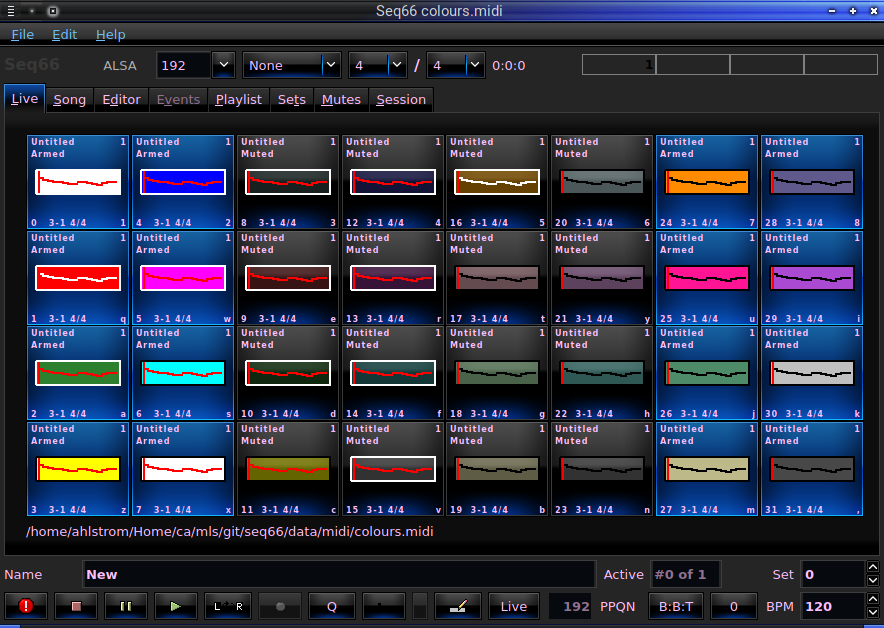
\includegraphics[scale=0.75]{main-window/main-window-fluxbox.png}
   \caption*{Seq66, Theme Dark-Cold Master, Fluxbox WaterDrops Style}
\end{figure}

\clearpage                             % moves Contents to next page

\tableofcontents
\listoffigures                         % print the list of figures
\listoftables                          % print the list of tables

% Changes the paragraph style to remove indenting and put a line between each
% paragraph.  This could be moved up into the preamble, but then would
% affect the spacing of the TOC and LOF, LOT noted above.

\setlength{\parindent}{2em}
\setlength{\parskip}{1ex plus 0.5ex minus 0.2ex}

\rhead{\rightmark}         % shows section number and section name

\section{Introduction}
\label{sec:introduction}

   This document describes "Seq66", a reboot of \textsl{Seq24} and a rewrite of
   \textsl{Sequencer64}, through version 0.97.2.
   The following project supports \textsl{Seq66} and documentation:

   \begin{itemize}
      \item \url{https://github.com/ahlstromcj/seq66.git}
   \end{itemize}

   \textsl{Seq66} is \textsl{Sequencer64} refactored for newer versions of
   \textsl{C++} with cruft cleanup.  It drops the
   \textsl{Gtkmm} user-interface in favor of \textsl{Qt 5},
   and has better handling of sets, mute-groups, sessions, configuration files,
   and more.
   It supports for the \textsl{Non Session Manager}, the ability to
   modify the color palette, and Qt style-sheets.
   Be prepared to note some significant differences
   between \textsl{Seq66} and \textsl{Sequencer64}.

   We also have many contributors to acknowledge.
   Please see \sectionref{sec:kudos}.
   It is out-of-date!  If your name is not there, ping us!

\subsection{Seq66: What!?}
\label{subsec:what_is_seq66}

   \textsl{Seq66} is a reboot of \textsl{Sequencer64}, which
   is itself a reboot of \textsl{Seq24},
   a live-looping sequencer with an interface similar to a hardware sequencer.
   \textsl{Seq66} is not a synthesizer.  It requires a hardware
   synthesizer or a software synthesizer.  It does not handle audio data,
   just MIDI.

   \textsl{Seq66} works with \textsl{ALSA}, \textsl{JACK},
   \textsl{PortMidi}, and \textsl{Windows}. It uses close-to-the-latest C++
   features for faster and simpler code.

\subsection{Seq66: Why!?}
\label{subsec:introduction_vs_others}

   The first reason to refactor \textsl{Sequencer64} is to take advantage of
   things learned in responding to user reports.  The second reason is to use
   the new code as an opportunity to add new functionality such as
   \textsl{Non Session Manager} support.  The third reason is to tighten the
   code by using newer features of \textsl{C++11} and later.
   The fourth reason is to make the innumerable minor improvements that come to
   attention with time and more testing.

\subsection{Improvements}
\label{subsec:improvements}

   The following improvements are some that have been made in
   \textsl{Seq66} versus \textsl{Sequencer64}.

   \begin{itemize}
      \item Qt 5 as the standard user-interface. Changing the window size works
         much better.
      \item A song editor tab for laying out patterns into a complete
         performance.
      \item A mutes editor tab, improvements to mutes handling, control, and
         status display.
      \item A playlist editor tab, with improved flexibility and automation.
      \item A sets editor tab.
      \item A events editor tab for basic fixing of minor event issues.
      \item A better live frame (main window and external windows) using
         Qt buttons.
      \item Non Session Manager support. A sessions tab which shows the current
         locations of configuration files for the run.
      \item Repartitioning of the configuration files into separate files for
         flexibility; added a color palette file, Qt style-sheets, beefed up the
         'ctrl' file radically.
      \item Improved alternate keyboard layout support.
      \item Mapping of port names to a consistent set of port numbers.
      \item Palette files and Qt style-sheets can be used to configure the colors
         of the painted text, lines, patterns, and the size and color of
         the user-interface items.
         Qt style-sheets can be useful in tweaking items, such as text in
         disabled controls that is difficult to see.
      \item More efficient lookups for controls; lambda functions.
   \end{itemize}

   For developers, a \textsl{Seq66} build is customizable via C macros,
   by enabling/disabling options at 'configure' time, and by many
   command-line arguments.  We cannot show all permutations of settings in this
   document, so don't be surprised if some screenshots don't quite match
   one's setup.  Distro maintainers might create their own build
   configurations.

\subsection{Document Structure}
\label{subsec:introduction_document_structure}

   The structure of this document follows the user-interface of
   \textsl{Seq66}.
   To help the reader jump around this document, it provides
   multiple links, references, and index entries.

\subsection{Building Seq66}
\label{subsec:introduction_building_seq66}

   There are a number of ways of building Seq66.

   \begin{itemize}
      \item Autotools Build and Install. Configure, make, and install.
      \item Bootstrap Install. Generate autotools files and build.
      \item OpenSUSE Tumbleweed. Specifics for that Linux distro.
      \item Qmake-based Install. Optional on Linux, mandatory for Windows.
      \item Windows Installer.  Currently in the sequencer64-packages site on
         GitHub.
   \end{itemize}

   The \texttt{INSTALL} file included with the source code and
   documentation goes into great detail about these methods.
   Also see \texttt{data/readme.windows} and \texttt{contrib/notes/git.txt}
   for supplemental information.

\subsection{Let's Go!}
\label{subsec:introduction_lets_go}

   Make sure no other sound application is running, for the first run.
   Start \textsl{Seq66} to use JACK for MIDI, or
   on \textsl{Windows}, just run it (\texttt{qseq66}, or \texttt{qpseq66.exe}
   on \textsl{Windows}); for better trouble-shooting, run it from
   the command-line at first.
   The port settings will depend on your system.
   Provide a MIDI file.
   On our system, the synthesizer (\textsl{Yoshimi}) comes up on MIDI buss 5;
   on \textsl{Windows}, buss 0 is the "MIDI Mapper", while buss 1 is the
   built-in wavetable synthesizer, which is normally under control of buss 0.
   The \texttt{-{}-buss} option remaps all events to the desired buss:

   \begin{verbatim}
      $ qseq66 --jack-midi --buss 5 data/midi/b4uacuse-gm-patchless.midi
      C:\> qpseq66 --buss 1  data/midi/b4uacuse-gm-patchless.midi
   \end{verbatim}

   If the \texttt{-{}-alsa} option is used instead of
   \texttt{-{}-jack-midi}, then the \textsl{ALSA} subsystem is used
   (Linux only).
   The buss setting can also be made via the port drop-down control
   in the main window.

   The "data" directory is a directory created upon installation of the
   application:

   \begin{verbatim}
      /usr/share/seq66-0.90/                       (Linux)
      C:/Program Files (x86)/Seq66/data            (Windows)
   \end{verbatim}

   Some of the files in those directories apply to both operating systems, so
   be sure to poke around and look.
   The configration files are stored in the user's "home" area:

   \begin{verbatim}
      /home/user/.config/seq66/qseq66.*            (Linux)
      C:/Users/user/AppData/Local/seq66/qpseq66.*  (Windows)
   \end{verbatim}

   The configuration files in the "home" directory
   are created after the first run of \textsl{Seq66}.

   For our walk-through of the main window, the following figure
   shows it using green labels and borders for reference.

\begin{figure}[H]
   \centering 
   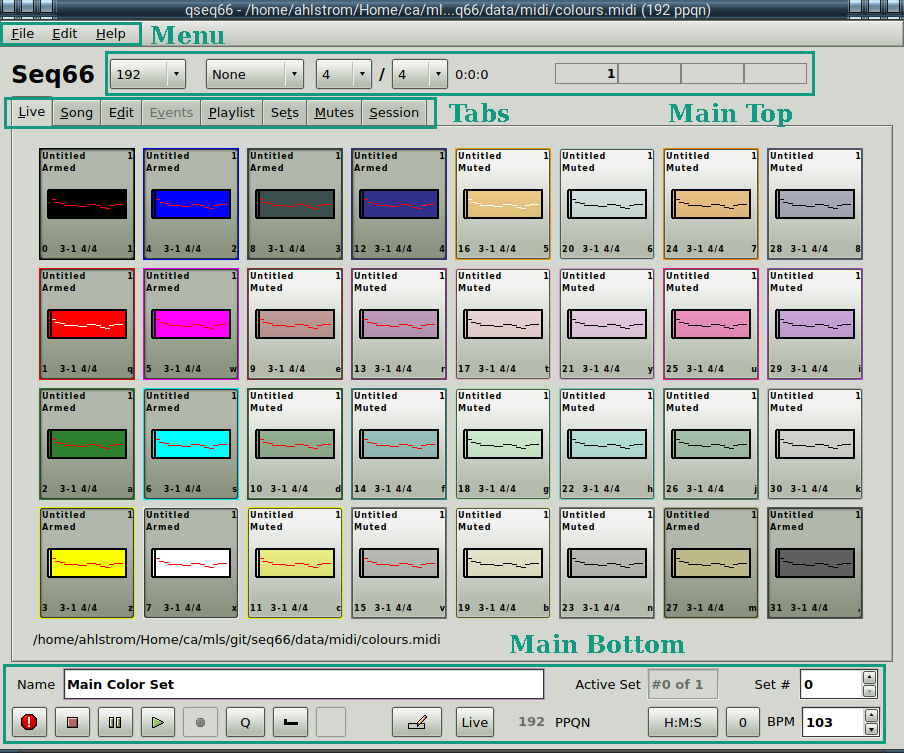
\includegraphics[scale=0.65]{main-window/main-window-light-gridstyle-3-markup.png}
   \caption{Seq66 Main Screen}
   \label{fig:main_screen}
\end{figure}

   The \textsl{Seq66} main window appears as shown above.
   This figure has many differences from the \textsl{Seq24} main window,
   but the functionality is similar.
   \textsl{Seq66} behaves better on resizing, and can also
   be configured to start with its size scaled up or scaled down.
   Most features, including the "look" of the application,
   can be configured via the 'rc', 'usr', 'ctrl', 'drums', 'playlist', 'mutes',
   and 'palette' configuration files, via command-line options, via
   desktop themes, and via Qt style-sheets ('qss' files).
%  There are many new front-panel items in \textsl{Seq66}.
%  Many of these buttons have configurable keystrokes and configurable MIDI
%  controls.

   We break the discussion into sections for the following
   groups shown in the figure above:

   \begin{itemize}
      \item \textbf{Tabs}
      \item \textbf{Menu}
      \item \textbf{Main Screen Controls}
   \end{itemize}

   The \textbf{Live} tab is foremost in the application.
   It provides a grid of \textsl{patterns}
   (also called \textsl{loops}, \textsl{tracks}, or
   \textsl{sequences}) that display recorded MIDI data, status information, and
   provide popup-menus for each pattern.
   The buttons can
   be colored via a palette, and the status of being armed is easy to see
   from the theme's coloring of activated buttons, and a label that says "Armed"
   versus "Muted".
   In addition, the buttons can be toggled by a keystroke, shown in the lower
   right corner of the button.
   Another name for the \textbf{Live} tab is the \textbf{Patterns Panel};
   it can be replicated in multiple external windows.
   This tab and all the other tabs
   will be discussed in more detail, each in its own section.
   The \textbf{Menu} is also described later (see \sectionref{sec:menu}).

   Here, we first discuss the top and bottom \textbf{Main} controls, as
   shown in the following collapsed figure:

\begin{figure}[H]
   \centering 
   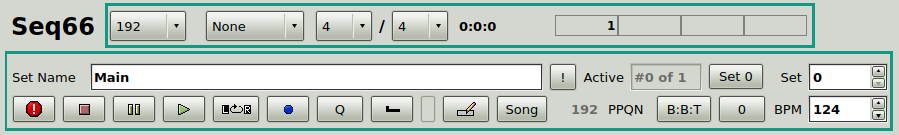
\includegraphics[scale=0.75]{main-window/main-window-controls.png}
   \caption{Main Screen Controls}
   \label{fig:main_screen_controls}
\end{figure}

   See the following section and
   \sectionref{subsubsec:introduction_main_bottom_controls}.

\subsubsection{Main Top Controls (Condensed View)}
\label{subsubsec:introduction_main_top_controls}

   The top panel of the Pattern window is simple, consisting of the
   name of the program and a few controls.
   The top main control items are, from left to right:

   \begin{itemize}
      \item \textbf{PPQN Selection}
      \item \textbf{Buss Override for Play-set}
      \item \textbf{Global Beats Per Measure}
      \item \textbf{Global Beat Width}
      \item \textbf{BBT or HMS Time Display}
      \item \textbf{Beat Indicator}
   \end{itemize}

   Not shown are some status indicators that can appear to the right of the
   "Seq66" logo:

   \begin{itemize}
      \item \textbf{ALSA} appears if running using ALSA for MIDI.
      \item \textbf{JACK} appears if running using JACK for MIDI.
      \item \textbf{Master} appears if running using JACK transport, as
         transport master.
         JACK transport can be used even if using ALSA for MIDI.
      \item \textbf{Slave} appears if using JACK transport as transport slave.
      \item \textbf{Portmidi} appears if using the internal portmidi-derived
         MIDI engine.  This is currently always the case on \textsl{Windows}.
   \end{itemize}

% Use this?
%  \setcounter{ItemCount}{0}
%  \itempar(PPQN Selection}{PPQN!selection}

\paragraph{PPQN Selection}
\label{paragraph:introduction_ppqn_selection}

   This drop-down allows one to change the pulses-per-quarter-note (PPQN) of the
   loaded tune, and this change can then be saved, if desired, with the file.
   As with \textsl{Seq24}, the default PPQN is 192.  This can be changed to
   to other values:
   \texttt{32, 48, 96, 192, 240, 384, 768, 960, 1920, 2400, 3840,
   7680, 9600, and 19200}.
   Values, even weird ones, can be entered by typing them.
   If a MIDI file is loaded, this modifies that file, rescaling all the
   pattern events and pattern triggers.
   Also see \sectionref{paragraph:menu_edit_preferences_play_options}.

\paragraph{Buss Override for Play-set}
\label{paragraph:introduction_sets_buss_override}

   This drop-down allows for overriding the buss (port) number used by all of
   the patterns in the current play-set.
   Unlike the \texttt{buss-override} setting in the 'usr' file
   (see \sectionref{subsubsec:usr_file_user_midi_settings}),
   this action causes a modification of the file (and a prompt to save at
   exit).

   \index{play-set}
   The \textsl{play-set} is the current set of patterns to be played.
   Normally, this set holds only the active patterns in the current
   play-screen.
   However, it can also be configured to include patterns from other sets.
   (See \sectionref{subsec:configuration_rc}.)

   The list of
   output busses is either the existing MIDI ports on the system, or,
   if port-mapping (see \sectionref{sec:port_mapping}) is active, the list
   of mapped output ports.
   Port-mapping is a useful way to redirect the set to a different output
   device; it can be used to provide a full set of virtual devices that any of
   the user's sequences can depend on.

   \index{--bus option}
   Another way to specify busses is the
   \texttt{-{}-buss n} command-line option.
   It causes \textsl{every} pattern in \textsl{every} set in the MIDI
   file to be directed to that buss number, and when a new
   sequence/pattern is created.  This option is only
   for convenience in testing.  Save the file, and it will
   have that buss number as part of each track's data, which makes the song
   file less portable, so be careful with both options.
   For portability, set the output buss to 0.

\paragraph{Global Beats Per Measure}
\label{paragraph:introduction_global_beats_per_measure}

   This drop-down changes the global beats/measure for the song.
   Along with the beat-width setting, this set of values allows
   for a large number of different time signatures, even crazy ones.

   Values: \texttt{1 to 16, 32}

\paragraph{Global Beat Width}
\label{paragraph:introduction_global_beat_width}

   This drop-down changes the global beat width (time-signature denominator)
   for the song.
   Along with the beats-per-measure setting, this set of values allows
   for a large number of different time signatures.

   Values: \texttt{1 to 16, 32}

\paragraph{BBT or HMS Time Display}
\label{paragraph:introduction_time_display}

   This text simply shows the current time during playback. 
   It can be shown in BBT (bars:beats:ticks) or HMS (hours:minutes:seconds)
   by clicking the \textbf{BBT/HMS} at the bottom of the window.

\paragraph{Beat Indicator}
\label{paragraph:introduction_beat_indicator}

   The beat indicator is inspired by the \textsl{Kepler34} implementation.
   It shows the first beat in color, and the rest of the beats in white.
   It does not adapt to changes in the time-signature until
   playback is stopped.

\subsubsection{Main Bottom Controls, First Row}
\label{subsubsec:introduction_main_bottom_controls}

   The bottom main control items take up two rows.
   The first row contains:

   \begin{itemize}
      \item \textbf{Set Name}
      \item \textbf{Set Reset ("!")}
      \item \textbf{Active Set Indicator}
      \item \textbf{Set 0}
      \item \textbf{Set Changer}
   \end{itemize}

\paragraph{Set Name}
\label{paragraph:introduction_set_name}

   This text field shows the name of the current set, and also allows editing
   the set name.

\paragraph{Set Reset ("!")}
\label{paragraph:introduction_set_reset}

   This small button with an exclamation point
   to the right of the set name is meant to clear
   out all playing sets, and make only the current set the playing set.
   This button is useful when in "all-sets" mode or when sets get added
   automatically via the "additive" mode, so that multiple sets are playing
   at once.
   See \sectionref{subsec:configuration_rc}.

\begin{comment}

% The Set Master button has been removed.

\paragraph{Set Master Button}
\label{paragraph:introduction_set_master_button}

   This button brings up an external window showing the \textbf{Set Master}
   panel.  This panel is also available in a center tab.  It is a work in
   progress, and doesn't have a whole lot of functionality yet.
   It can currently show existing sets in one view, and allow
   reordering the sets.

\end{comment}

\paragraph{Active Set Indicator}
\label{paragraph:introduction_active_set_indicator}

   This read-only text field shows the set number of the currently active set.
   One can open a number of external \textsl{Live Frames} by
   Shift-left-clicking on pattern slots.  The currently active set is then the
   set that has the mouse focus.  This allows for working with multiple sets
   without a lot of mouse/keyboard navigation.

\paragraph{Set 0}
\label{paragraph:introduction_set_zero}

   This button provides a fast way to get back to set 0, without clicking the
   mouse a bunch of times.
   It is useful when creating an external live grid
   (see \sectionref{fig:multiple_live_grids}),
   which currently also sets the main grid to the same set.
   Click on this button, and the external set and set 0 can be seen at the same
   time.

\paragraph{Set Changer}
\label{paragraph:introduction_set_changer}

   This spin-box allows showing a different set in the main windows.
   This set can be modified by adding new patterns, changing its name, or
   importing other MIDI files into the current set.

\subsubsection{Main Bottom Controls, Second Row}
\label{subsubsec:introduction_main_bottom_controls_2}

   On to the next section of the main bottom buttons, the second row contains:

   \begin{itemize}
      \item \textbf{Panic Button}
      \item \textbf{Stop Button}
      \item \textbf{Pause Button}
      \item \textbf{Play Button}
      \item \textbf{Loop Button} (not shown, new since 0.93.0)
      \item \textbf{Live Record}
      \item \textbf{Keep Queue Button}
      \item \textbf{Mute Group Learn Button}
      \item \textbf{Developer Test Button}
      \item \textbf{Song Editor Button}
      \item \textbf{Song Mode Button}
      \item \textbf{PPQN Indicator}
      \item \textbf{BBT/HMS Toggle Button}
      \item \textbf{Tap BPM Button}
      \item \textbf{Beats Per Minute Control}
   \end{itemize}

   Many of these controls have keystrokes and MIDI-control slots that can be
   set up in the 'ctrl' file.

\paragraph{Panic Button}
\label{paragraph:introduction_panic_button}

   This button causes playback to stop, all patterns to mute, and flushes the
   MIDI buss.
   There is a keystroke control and a MIDI control
   for this automation operation, plus
   a MIDI-announcement (output) configuration item for it.

\paragraph{Stop Button}
\label{paragraph:introduction_stop_button}

   This button stops playback and rewinds to the beginning of the song.
   By default, the \texttt{Esc} key operates this function,
   and there is both a MIDI-control slot and a MIDI-announcement slot
   available for it.

\paragraph{Pause Button}
\label{paragraph:introduction_pause_button}

   This button stops playback, but does not rewind to the beginning of the song.
   It also resumes playback at the same point as the pause.
   By default, the \texttt{Period} key operates this function,
   and there is a MIDI-control slot and a MIDI-announcement slot available for it.
   This key is also hardwired to pause and start playback in the pattern editor and
   the song editor.

\paragraph{Play Button}
\label{paragraph:introduction_play_button}

   This button starts playback, either at the beginning or at the pause point.
   Also called the "start button".
   By default, the \texttt{Space} key operates this function,
   and there is both a MIDI-control slot and a MIDI-announcement slot
   available for it.
   This key is also hardwired to toggle playback in the pattern editor and the
   song editor.

\paragraph{Loop Button}
\label{paragraph:introduction_loop_button}

   This button has been added to the main window as of version 0.93.0 of
   \textsl{Seq66}.
   This reflects that the \textbf{L/R} loop markers in the song editor can now
   be used in the pattern editor as well.  This new feature makes it easier to
   focus in on a pattern and tinker repeatedly with the same small section.
   In addition, looping can now be done in both the Live and Song modes of
   playback.

\paragraph{Live Record Button}
\label{paragraph:introduction_live_record_button}

   This button causes a live playing session to be recorded.
   That is, triggers are added to the song automatically as the musician mutes
   and unmutes patterns, and the triggers can then be
   seen as layouts in the \textsl{Song} editor.
   By default, the \texttt{P} key operates this function,

\paragraph{Keep Queue Button}
\label{paragraph:introduction_keep_queue_button}

   Puts the application into a "sticky" queue mode.
   In this mode, pressing a pattern key does not do a mute/unmute function, but
   instead turns on queuing for the selected pattern.
   By default, the \texttt{Backslash} key operates this function,
   and there is a MIDI-control slot available for it.

\paragraph{Mute Group Learn Button}
\label{paragraph:introduction_mute_group_learn_button}

   Also called the "L" button.
   Sets up to learn the current set of active patterns ("mute group") into a
   mute-group.
   When in group-learn mode, the \texttt{Shift} key cannot be hit, so the
   group-learn mode automatically converts the keys to their shifted versions.
   This feature known as \textsl{shift-lock} or \textsl{auto-shift}.
   After pressing the "L" button, the user can then press a keystroke, which is
   automatically shifted, and the pattern set is saved, and can be recalled by
   that button (shifted) later.  It can be saved in a 'mutes' file, as part of
   the MIDI tune, or in both places.

   \textsl{Example}:
   We have 5 patterns armed in the current set. Press the "L" button,
   and then press the "s" key.  These pattern statuses are saved and can be
   recalled later by the "S" ("s"-shifted) key.

   By default, the \texttt{el} (lower-case "l") key also sets this function,
   and there is a MIDI-control slot available for it, as well as a
   MIDI-announcement slot.
   In addition to that, one can also press
   the \texttt{Ctrl-L} key.
   The "el" with it!

   Remember that groups work with the playing ("in-view") screen-set.
   One must change the screenset and give it the command to make it the
   playing one.
   \index{keys!Home}
   By default, the \texttt{Home} key is configured for this purpose.

   There is also a setting in the 'mutes' file called
   \texttt{mute-group-selected}.  If this value is set to a value from 0 to 31,
   then that mute group will be automatically applied when
   \textsl{Seq66} starts up.
   This is useful with the loading of the most-recent MIDI file (which is also
   a feature of \textsl{Seq66}.

   Also see \sectionref{sec:mutes_master}.

\paragraph{Developer Test Button}
\label{paragraph:introduction_developer_test_button}

   This button is always disabled.  Functionality is added temporarily when
   testing new features. Ignore this button.

\paragraph{Song Editor Button}
\label{paragraph:introduction_song_editor_button}

   This button (with a "pencil" icon)
   brings up an external window for editing the Song/Performance
   information.  If already up, it closes it.  Works the same as the
   \textbf{Edit / Song Editor} menu or the hard-wired \texttt{Ctrl-E} key.

\paragraph{Live/Song Mode Button}
\label{paragraph:introduction_livesong_mode_button}

   This button toggles between the \textsl{Live} and \textsl{Song} performance
   mode. In the Live mode, the musician controls are muting/unmuting of each
   pattern.  In the Song mode, the triggers layed out in the
   \textbf{Song Editor} control the playback.
   By default, the \texttt{F10} key operates this function,
   There is also a MIDI automation control for this button.

\begin{comment}
   \itempar{Toggle Tracks}{pattern!toggle tracks}
   \index{pattern!toggle tracks}
   This button changes the status of all of the
   \textsl{playing} tracks, reversing the
   mute status of each pattern that is playing.
   The next click will then unmute only those tracks.
   Because it can be confusing, this button is disabled (not shown
   in the figure) in Song mode.

   LATER:  Describe
   \texttt{Ctrl-M},
   \texttt{Ctrl-U}, and
   \texttt{Ctrl-T}.

\end{comment}

\paragraph{PPQN Indicator}
\label{paragraph:introduction_ppqn_indicator}

   This read-only field displays the current PPQN for the current tune.

   \configref{usr}{user-midi-settings}{midi\_ppqn}

\paragraph{BBT/HMS Toggle Button}
\label{paragraph:introduction_time_format_toggle_button}

   Toggles the format of the current time displayed during playback. 
   It can be shown in B:B:T (bars:beats:ticks) or H:M:S (hours:minutes:seconds).

\paragraph{Tap BPM Button}
\label{paragraph:introduction_tap_bpm_button}

   Tap this button with a regular beat to determine the beats-per-minute of the
   tapping.  With each tap, the counter on the button increments and the BPM is
   recalculated.  Stop tapping for a few seconds to reset the counter.
   By default, the \texttt{F9} key operates this function, but it
   STILL NEEDS WORK to show the results in the BPM control.
   There is also a MIDI-control slot for this function.

\paragraph{Beats Per Minute Control}
\label{paragraph:introduction_bpm_control}

   This control can be text-edited or spun to change the beats/minute value
   used in playing back the current song.  This value is also saved to the
   file.

%     \item Log Tempo, which inserts the current tempo into the tempo track
%        as an event.
%     \item Tempo recording, which inserts all tempo changes as tempo events.

% Menu

%-------------------------------------------------------------------------------
% menu
%-------------------------------------------------------------------------------
%
% \file        menu.tex
% \library     Documents
% \author      Chris Ahlstrom
% \date        2015-08-31
% \update      2024-12-03
% \version     $Revision$
% \license     $XPC_GPL_LICENSE$
%
%     Provides the Menu section of seq66-user-manual.tex.
%
%-------------------------------------------------------------------------------

\section{Menu}
\label{sec:menu}

   The \textsl{Seq66} menu structure is more complex than
   that of \textsl{Seq24}.  In particular, the \textsl{File} menu has two
   variants:  a normal file menu, and a file menu when \textsl{Seq66} is
   running under the \textsl{New/Non Session Manager}.
   (See \sectionref{subsec:sessions_nsm}.)

\subsection{Menu / File}
\label{subsec:menu_file}

   The \textbf{File} menu is used to save and load files in
   Standard MIDI Format 0 or 1, \textsl{Cakewalk} "WRK",
   and \textsl{Seq66} MIDI files.
   It also supports a list of recent files, and (new with version 0.98.3)
   sub-menus for import and export functions, which have expanded quite a bit.

   The \textsl{Seq66} \textbf{File} menu contains the sub-items shown below.
   The next few sub-sections discuss
   the sub-items in the \textbf{File} menu.
   Please note that these entries are different
   if \textsl{Seq66} is started under the control of the
   \textsl{New/Non Session Manager}.  
   See \sectionref{subsubsec:sessions_file_menu}.
   However, the import and export menus remain the same, although there are
   slight differences in how they work.

\begin{figure}[H]
   \centering 
   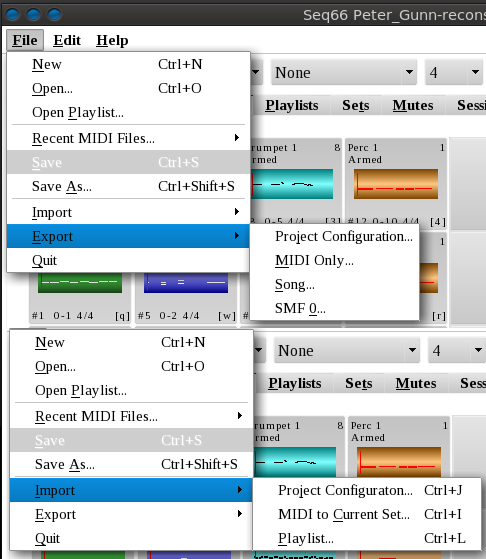
\includegraphics[scale=0.75]{main-menu/file/file-import-export-menus.png}
   \caption{Seq66 File Menu Plus Import/Export, Composite View}
   \label{fig:menu_file_items}
\end{figure}

   \begin{enumber}
      \item \textbf{New}
      \item \textbf{Open}
      \item \textbf{Open Playlist}
      \item \textbf{Recent MIDI files}
      \item \textbf{Save}
      \item \textbf{Save As}
      \item \textbf{Import}
      \begin{enumber}
         \item \textbf{Project Configuration...}
         \item \textbf{MIDI to Current Set...}
         \item \textbf{Playlist...}
         \index{restart!automatic}
         Once the playlist is imported,
         \textsl{Seq66} is automatically \textsl{\textbf{restarted}}
         in order to load the playlist.
         Be careful!
      \end{enumber}
      \item \textbf{Export}
      \begin{enumber}
         \item \textbf{Project Configuration...}
         \item \textbf{MIDI Only...}
         \item \textbf{Song...}
         \item \textbf{SMF 0...}
      \end{enumber}
      \item \textbf{Quit} (\textbf{Exit} in \textsl{Windows})
   \end{enumber}

   For information on the \textbf{File} menu when \textsl{Seq66} is
   running under the \textsl{Non Session Manager}, see
   \sectionref{subsubsec:sessions_file_menu}.

\subsubsection{Menu / File / New}
\label{subsec:menu_file_new}

   The \textbf{New} menu entry clears the current song.
   (A play-list or mute-groups setup, if loaded, are not affected.)
   If unsaved changes are pending, the user is prompted to save the changes.
   Prompting for changes is more comprehensive than \textsl{Seq24}.
   However, when in doubt, save!
   Keep backups of your tunes and configuration files!

\subsubsection{Menu / File / Open}
\label{subsubsec:menu_file_open}

   The \textbf{Open} menu entry opens a song (MIDI file or \textsl{Cakewalk}
   WRK file), replacing the current song (after a prompt if the song was
   modified).
   It opens up a standard file dialog:

\begin{figure}[H]
   \centering 
   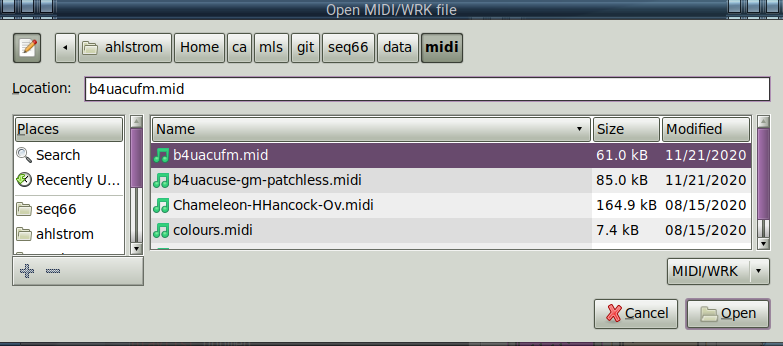
\includegraphics[scale=0.65]{main-menu/file/light-menu-file-open.png}
   \caption{File / Open}
   \label{fig:menu_file_open}
\end{figure}

   This dialog lets one type a file-name, highlighting the first file
   that matches the characters typed.
   \textsl{Seq66} can open \textsl{Seq66}, MIDI SMF 0, and SMF 1 files, and
   \textsl{Cakewalk} WRK files.
   If the file is an SMF 0 file, where all channels appear on one track, the
   track is split so that each channel (0 to 15) is stored in the corresponding
   pattern, and pattern 16 contains the original track.

   Note that a MIDI file can be drag-and-dropped from a file manager onto
   the grid to open a file.

\subsubsection{Menu / File / Open Playlist}
\label{subsubsec:menu_file_open_playlist}

   The \textbf{Open Playlist...} menu entry opens a \textsl{Seq66}
   play-list file.

\begin{figure}[H]
   \centering 
   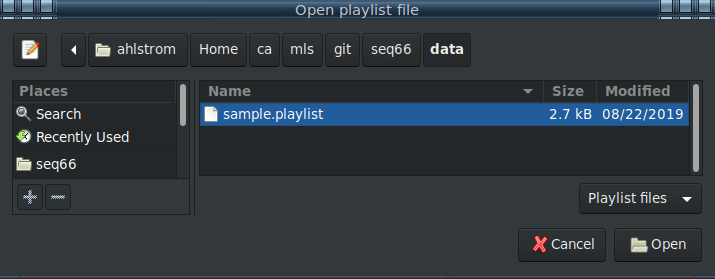
\includegraphics[scale=0.65]{main-menu/file/dark-menu-file-open-playlist.png}
   \caption{File / Open Playlist}
   \label{fig:menu_file_open_playlist}
\end{figure}

   The playlist file contains a list of "playlist sections",
   each listing a number of MIDI songs.
   These playlists and songs can be
   selected by the arrow keys or by MIDI control,
   and are displaed and editiable in the \textsl{Playlist} tab
   in the main window.
   See \sectionref{sec:playlist}.

\subsubsection{Menu / File / Recent MIDI files}
\label{subsubsec:menu_file_recent}

   This menu entry provides a list of the last few MIDI files created or opened;
   play-list selections are \textsl{not} included in this list.

\begin{figure}[H]
   \centering 
   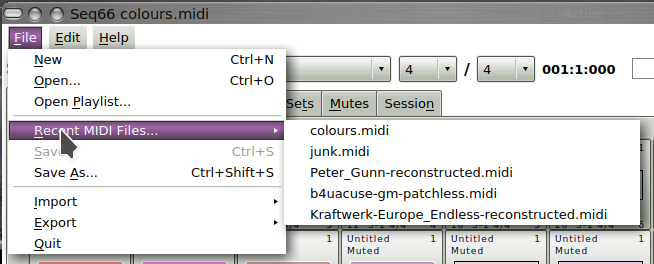
\includegraphics[scale=0.65]{main-menu/file/menu-recent-files.png}
   \caption{Seq66 Menu File Recent Files}
   \label{fig:menu_file_recent_files}
\end{figure}

   Here is the long form when the 'rc' file's
   \texttt{[recent-files] full-paths} value is set to true:

\begin{figure}[H]
   \centering 
   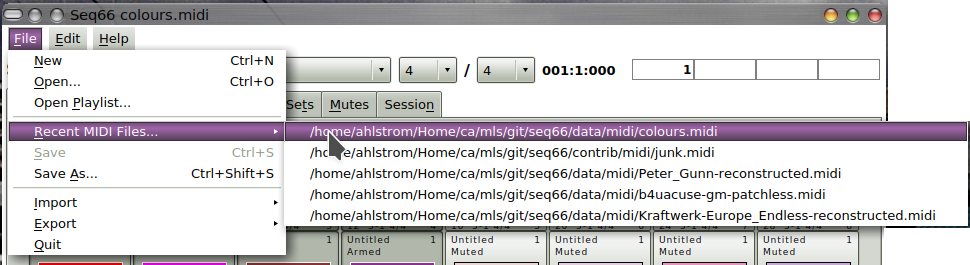
\includegraphics[scale=0.65]{main-menu/file/menu-recent-files-long.png}
   \caption{Seq66 Menu File Recent Files, Full Paths}
   \label{fig:menu_file_recent_files_full_paths}
\end{figure}

   This list is saved in the \texttt{[recent-files]} section of the
   'rc' configuration file.
   In the 'rc' file, the full path to the file-name is stored.
   This path is in "UNIX" format, using the forward slash, or solidus,
   as the path separator, even in \textsl{Windows}.
   The \texttt{full-paths} option can be set to show the full path in the
   recent-files drop-down menu.
   Only unique entries are included in the recent-files list.
   The limit is 12 recent-file entries.
   This is a feature from \textsl{Kepler34} \cite{kepler34}.
   One can also set \textsl{Seq66} to load the most-recent file at startup.
   Here is an example from an 'rc' file:

\begin{verbatim}
   [recent-files]
   full-paths = false
   load-most-recent = true
   count = 3
   /home/user/git/seq66/data/b4uacuse-gm-patchless.midi
   /home/user/git/seq66/data/midi/colours.midi
   /home/user/git/Julian-data/TestBeeps.midi
\end{verbatim}

\subsubsection{Menu / File / Save and Save As}
\label{subsubsec:menu_file_open_save_as}

   The \textbf{Save} menu entry saves the song under its current file-name.
   If there is no current file-name, it opens up a standard file
   dialog to name and save the file.
   The \textbf{Save As} menu entry saves a song under a different name.
   It opens up the following standard file dialog, very similar to the 
   \textbf{File Open} dialog, with an additional \textbf{Name} text-edit field.

\begin{figure}[H]
   \centering 
   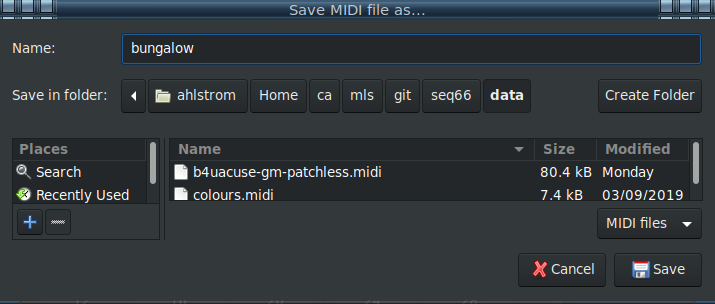
\includegraphics[scale=0.65]{main-menu/file/dark-menu-file-save-as.png}
   \caption{File / Save As}
   \label{fig:menu_file_save_as}
\end{figure}

   To save a new file or save the current file to a new name,
   enter the name in the name field, without an extension.
   \textsl{Seq66} will append a \texttt{.midi} extension to the filename.
   The file will be saved in a format that the Linux \textsl{file} command
   will tag as something like:

   \begin{verbatim}
      colours.midi: Standard MIDI data (format 1) using 16 tracks at 1/192
   \end{verbatim}

   It looks like a simple MIDI file, and yet, if one re-opens it in
   \textsl{Seq66}, one sees that the mute-groups, labeling, pattern
   information, and song layout have been preserved in this file.
   This information is saved in a way that MIDI-compliant software
   should be able to use or ignore without failure.
   After the last track in the file, a number of
   \index{SeqSpec}
   sequencer-specific (SeqSpec) items are saved, to preserve
   the extra information that \textsl{Seq66} adds to the song.
   There is no way to save a \textsl{Cakewalk} "WRK" file.
   \textsl{Seq66} can only read them, and then save them as
   \textsl{Seq66} files.

   \index{Meta events}
   Meta events are now partially handled by \textsl{Seq66}.
   Meta events \textbf{Set Tempo}
   and \textbf{Time Signature}
   are now fully supported.
   Other meta events,
   such as \textbf{Meta MIDI Channel}
   and \textbf{Meta MIDI Port}
   are now read as events, and are saved back when the file is saved.
   They cannot be edited in \textsl{Seq66}, but they are not lost.
   (Channel and port meta events are
   considered \textsl{obsolete} in the MIDI standard.)
   Lastly, various meta text events, such as \textbf{Lyric},
   can be edited and saved.

\subsubsection{Menu / File / Import / Project Configuration}
\label{subsubsec:menu_file_import_project_configuration}

   This command is useful to grab an existing project configuration
   (i.e. the set of \texttt{qseq66.*} files) and copy it
   to another directory.
   This command is most useful in importing a project into a new
   NSM session.  Previously, the "home" project would be imported automatically
   into a new NSM session, but this was deemed confusing by some users, and
   properly so!

   This command brings up a file dialog box. Navigate to the desired
   source directory and then select the desired 'rc' file.
   This saves and rereads the configuration.
   If importing into a normal (i.e. not NSM) session, \textsl{Seq66} will
   restart itself automatically to save and reread the configuration.
   Be aware!
   For more information, see
   \sectionref{subsubsec:midi_export_file_import_project}.

\subsubsection{Menu / File / Import / MIDI to Current Set}
\label{subsubsec:menu_file_import}

   The \textbf{Import} menu entry imports an SMF 0
   or SMF 1 MIDI file as one or more patterns, one pattern per track,
   into the specified screen-set.
   This functionality is explained in detail in
   \sectionref{subsubsec:midi_export_file_import}.

\subsubsection{Menu / File / Import / Playlist}
\label{subsubsec:menu_file_import_playlisMIDI to Current Sett}

   A user can create a playlist that accesses MIDI files anywhere in the file
   system.
   However, in a session manager, it is preferable to have the configuration
   self-contained.
   Even without a session manager, it can be useful to copy a playlist to a
   subdirectory in order to separate it and its MIDI files from other
   playlists.
   Once a project has been imported or saved, then a playlist can also be
   imported, along with all of the MIDI files it references.

   This command brings up a file dialog box. Navigate to the desired
   source directory and then select the desired 'playlist' file.
   This menu entry copies the playlist file and its associated
   MIDI files; see
   \sectionref{subsubsec:midi_export_file_import_playlist}.

\subsubsection{Menu / File / Export / Project Configuration}
\label{subsubsec:menu_file_export_project}

   This menu entry lets the user select a destination directory.
   Then the project files from the current "home" directory are copied
   to that destination directory. Useful for backup.
   See \sectionref{subsubsec:midi_export_configuration_export}.

\subsubsection{Menu / File / Export / Song}
\label{subsubsec:menu_file_export_song_as_midi}

   Thanks to the \textsl{Seq32} project, the ability to export songs to MIDI
   format has been added.  In this export, a complete song performance is
   recoded so that other MIDI sequencers can play the performance properly.
   This functionality is explained in detail in
   \sectionref{subsubsec:midi_export_song_export}.

\subsubsection{Menu / File / Export / MIDI Only}
\label{subsubsec:menu_file_export_midi_only}

   Sometimes it might be useful to export only the non-vendor-specific
   (non-SeqSpec) data from a \textsl{Seq66} song, in order to reduce the
   size of the file or to accomodate non-compliant sequencers.
   This functionality is explained in detail in
   \sectionref{subsubsec:midi_export_file_export_midi_only}.

\subsubsection{Menu / File / Export / SMF 0}
\label{subsubsec:menu_file_export_smf_0}

   This feature is new since version 0.97.  It allows all tracks in the song to
   be consolidated and exported in MIDI's SMF 0 format.  It follows the same
   rules as song export.
   See \sectionref{subsubsec:midi_export_file_export_smf_0}.

\subsection{Menu / Edit}
\label{subsec:menu_edit}

   The \textbf{Edit} menu has undergone some expansion in \textsl{Seq66}.

   \begin{enumber}
      \item \textbf{Preferences...}
      \item \textbf{Song Editor}
      \item \textbf{Apply Song Transpose}
      \item \textbf{Clear Mute Groups}
      \item \textbf{Reload Mute Groups}
      \item \textbf{Mute All Tracks}
      \item \textbf{Unute All Tracks}
      \item \textbf{Toggle All Tracks}
      \item \textbf{Copy Current Set}
      \item \textbf{Paste To Current Set}
   \end{enumber}

   \setcounter{ItemCounter}{0}      % Reset the ItemCounter for this list.

   \itempar{Preferences}{edit!preferences}
   This entry brings up a \textbf{Preferences} menu entry,
   to allow viewing and tweaking MIDI I/O ports, displays options, JACK
   options, and more.
   It can also be brought up by \texttt{Ctrl-P}.
   It is discussed in detail in a later section.

   \itempar{Song Editor}{edit!song editor}
   \index{performance editor}
   \index{song editor}
   This item toggles the presence of the main song/performance editor.
   Note that the song editor is also available in the
   \textbf{Song} tab in the main window.
   The song/performance editor allows specifying exact numbers of loop replays;
   this provides a canned rendition of the MIDI tune.

   \itempar{Apply Song Transpose}{edit!song transpose}
   \index{song transpose}
   Selecting this item applies the global song transposition value to
   all sequences / patterns marked as transposable.
   This actively changes the note / pitch value of all note and aftertouch
   events in the pattern.
   Normally, drum tracks are \textsl{not} transposable.
   For the setting of global song transpose, see
   \sectionref{sec:song_editor}.
   Note that transpose can be enabled in the
   in the sequence editor
   (see \sectionref{sec:pattern_editor}).

   \itempar{Clear Mute Groups}{edit!clear mute groups}
   \index{mute groups}
   A feature of \textsl{Seq66} is that the mute groups
   are saved in both the 'rc' file \textsl{and} in the "MIDI" file.
   This menu entry clears them. If this resulted in any mute-group sequences
   status being set to false, then the user is prompted to save the MIDI
   file, so that it will no longer have any
   mute-group information.  And then, if the
   application exits, the cleared mute-group information is also saved to
   the 'rc' file.

   \itempar{Reload Mute Groups}{edit!load mute groups}
   \index{rc!mute groups}
   This menu entry reloads the mute-groups from the 'rc' file.
   So, if one loads a MIDI file that has its own mute groups that one does not
   like, this command will restore one's favorite mute-grouping from the 'rc'
   file.

   \itempar{Mute All Tracks}{edit!mute all tracks}
   \index{mute all}
   This menu entry, useful mostly in \textbf{Live} mode,
   immediately mutes \textsl{all} patterns in the entire song.
   The hard-wired keyboard short-cut for this action is \texttt{Ctrl-M}.

   \itempar{Unmute All Tracks}{edit!unmute all tracks}
   \index{unmute all}
   This menu entry, useful mostly in \textbf{Live} mode,
   immediately unmutes \textsl{all} patterns in the entire song.
   The hard-wired keyboard short-cut for this action is \texttt{Ctrl-U}.

   \itempar{Toggle All Tracks}{edit!toggle all}
   \index{toggle all}
   This option toggles the mute/armed status of \textbf{all} tracks.
   It is useful mostly \textbf{Live} mode, which overrides \textbf{Song}
   mode even if the Song Editor is focussed.
   The hard-wired keyboard short-cut for this action is \texttt{Ctrl-T}.

   \itempar{Copy Current Set}{edit!copy set}
   \index{copy set}
   This item marks the current set (i.e. the play-set)
   for the copying of all its patterns to another set.
   After clicking this menu entry, one can move to another set to paste it,
   using the following menu entry.

   \itempar{Paste To Current Set}{edit!paste set}
   \index{paste set}
   Once a set has been copied into the internal set clipboard,
   then this menu item is enabled.
   Move to the desired set (whether empty or note), and then
   click this menu item.
   All of the patterns in the original set are pasted into the current set,
   \textsl{overwriting all patterns} already in the set.
   Also note that the set clipboard can be pasted after a
   \textbf{File / New} or \textbf{File / Open},
   to copy it to another file.

\subsubsection{Menu / Edit / Preferences}
\label{subsubsec:menu_edit_preferences}

   \textbf{Preferences} provides a number of settings in one
   tabbed dialog, shown in the figures that follow.
   It allows one to set MIDI clocking, MIDI Input, display tweaks, minor
   playback options, and some JACK parameters.

  Configuration items not (yet) implemented in \textbf{Preferences} are
      incoming MIDI events to control the sequencer;
      what keys are mapped to functions;
      how the mouse works, and a few other.
   The MIDI and Key controls, far more numerous than in \textsl{Seq24}, have
   been consolidated into a 'ctrl' file and are fairly easy to edit with a text
   editor.
   \textsl{Seq66} does not support the 'fruity' mouse mode at this time.
   If you want it, ask us!

\paragraph{Menu / Edit / Preferences / MIDI Clock}
\label{paragraph:menu_edit_preferences_midi_clock}

   \textbf{Note}:
   \textsl{The MIDI Clock tab is sometimes difficult to click on.}
   We are not sure why.  It seems to be theme-dependent.
   In some things the tab thumb changes color when it can work.
   Just keep clicking in various locations in the tab,
   or use the \texttt{Alt-C} key.
   Weird.

   The \textbf{MIDI Clock} tab provides a way to set MIDI clocking for
   the available MIDI output busses.
   It configures the output busses for MIDI clock and data.
   It shows the devices that can play music.
   The items that appear in this tab depend on:

   \begin{itemize}
      \item What MIDI devices are connected to the computer.
         MIDI controllers, USB MIDI cables, applications with virtual
         ports, and other connected devices will add MIDI
         output devices (ports) to the system.
         This list will generally match the output of \texttt{aplaymidi -l}
         or \texttt{aconnect -lio}.
      \item The setting of the "manual-ports" option, which tells
         \textsl{Seq66} to set up virtual MIDI ports.
         It is enabled by the
         \texttt{-{}-manual-ports} command-line option or the
         \texttt{[manual-ports]} section of the
         \texttt{qseq66.rc} configuration file,
         or in the \textbf{MIDI Input} tab described below.
      \item The setting of the \textsl{Seq66}-specific
         "reveal ALSA ports" option,
         \texttt{-{}-reveal-ports} command-line option or the
         \texttt{[reveal-ports]} section of the
         \texttt{qseq66.rc} configuration file.
   \end{itemize}

   If \texttt{-{}-manual-ports} is on, this list shows the virtual
   MIDI output busses that \textsl{Seq66} can drive.
   One needs to use a JACK or ALSA MIDI
   connection application to connect a device on each of those outputs.
   The fact that the the buss names can
   start with different numbers, depending on the system setup, can complicate
   the playing of MIDI in this manner.  Also, the 'usr' configuration file can
   change the visible names of the ports to match specific equipment attached
   to the ports.

\begin{figure}[H]
   \centering 
   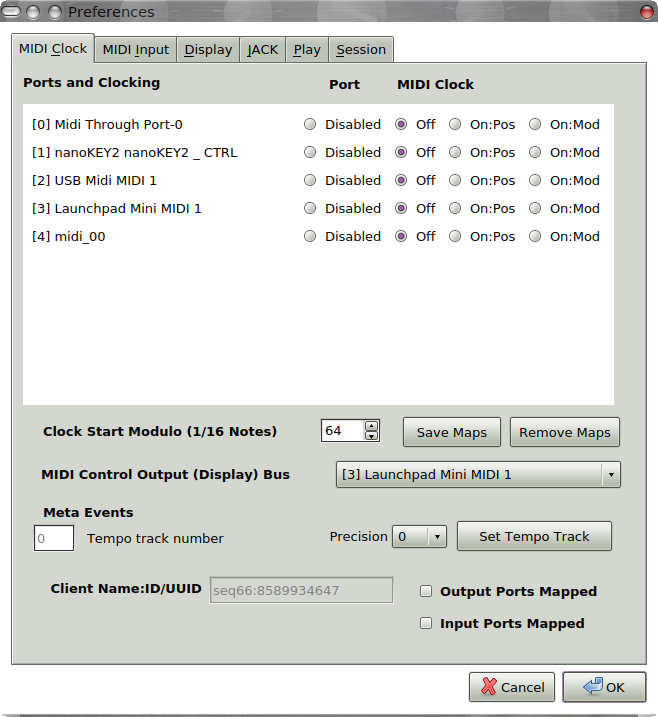
\includegraphics[scale=0.50]{main-menu/edit/preferences/midi_clock_tab.png}
   \caption{MIDI Clock (Output) Tab}
   \label{fig:midi_clock_tab}
\end{figure}

   This diagram is slightly out-of-date, but we go forward!
   It shows the tab for configuring MIDI output and clocking features.

   \begin{quotation}
      \textbf{Tip}:
      With some Qt themes, it is difficult to activate this tab by clicking
      because there is little or no sensitive area on the tab.
      In this case, click \texttt{Alt-c} once or twice.
   \end{quotation}

   Port-mapping is the default, and when active, is shown in this pane.
   If there are more than about a dozen
   output ports in the system, then a vertical scrollbar appears.
   The following elements are present in this tab:

   \begin{enumber}
      \item \textbf{Ports and Clocking Table}
      \item \textbf{Clock Start Modulo}
      \item \textbf{Buss Override}
      \item \textbf{MIDI I/O Maps}
      \item \textbf{Create (maps)}
      \item \textbf{Clear (maps)}
      \item \textbf{MIDI Control Output Bus}
      \item \textbf{Meta Events}
      \item \textbf{Client Name:ID/UUID}
      \item \textbf{Restart Seq66!}
   \end{enumber}

   \setcounter{ItemCounter}{0}      % Reset the ItemCounter for this list.

   \itempar{Ports and Clocking}{output!ports and clocks}
   \index{output ports}

   This table shows the available MIDI outputs and their status.
   If the set of system MIDI devices and software devices has changed since
   the last run, this list could be in error.  Restart the application
   and see if it is now correct.  Currently, there is no way to edit the list
   except in the 'rc' file.

   The \textbf{Ports and Clocks} table contains the following elements,
   although some can be removed by specifying the
   \texttt{port-naming = short} option in the 'rc' file.

   \begin{enumber}
      \item \textbf{Index Number}
      \item \textbf{Client Number}
      \item \textbf{Port Number}
      \item \textbf{Buss Name}
      \item \textbf{Port Disabled}
      \item \textbf{Off}
      \item \textbf{On (Pos)}
      \item \textbf{On (Mod)}
      \item \textbf{Clock Start Modulo}
   \end{enumber}

   The format of the left side of the entry listing is like the following
   when the port-naming option is "long", and the
   MIDI subsystem is ALSA):

   \begin{verbatim}
      [5] 128:4 yoshimi:input
       ^  ^   ^ ^        ^
       |  |   | |        |
       |  |   | |         ---- Port/buss name
       |  |   |  ------------- Client name
       |  |    --------------- Port/buss number
       |   ------------------- Client number
        ---------------------- Index number
   \end{verbatim}

   \setcounter{ItemCounter}{0}      % Reset the ItemCounter for this list.

   \itempar{Index Number}{midi clock!index number}
   \index{index number}
   The number in square brackets is an ordinal indicating the position
   of the output buss in the list.
   For all practical purposes in \textsl{Seq66}, it \textsl{is} the
   buss/port number.  This number can be stored in a pattern in order to have
   the pattern's output go to that buss.  
   This is true even if port-mapping is in place.
   \index{port!mapping}
   \index{buss!mapping}
   \index{port!override}
   \index{buss!override}
   It can be used with the \texttt{-b},
   \texttt{-{}-buss}, or \texttt{ -{}-bus} options to redirect all
   pattern output to that buss, useful if only one buss is active or the
   \textsl{Seq66} patterns route to non-existent busses.
   (See \sectionref{subsubsec:introduction_sets_buss_override},
   and \sectionref{subsubsec:usr_file_user_midi_settings}.)

   \itempar{Client Number}{midi clock!client number}
   \index{client number}
   The number that precedes the colon is the "client number".
   It is useful mainly in ALSA, where clients can have numbers like "14",
   "128", "129", etc.  For native JACK mode, it matches the index number or is
   the name of the client (e.g. "seq66").

   \itempar{Port Number}{midi clock!port number}
   \index{port number}
   The number that follows the colon is the "port number".
   It is useful mainly in ALSA.
   For native JACK mode, it matches the index number.

   \itempar{Buss Name}{midi clock!buss name}
   \index{port name}
   \index{midi clock!port name}
   These labels indicate the output busses (ports) available.
   \textsl{Seq66} does not access devices by name, but by port number.
   However, a port-map can be created to make it possible to find the correct
   buss / port number by name lookup.

   \itempar{Port Disabled}{midi clock!port disabled}
   The \textbf{Port Disabled} clock choice marks an output port
   that the user does not want to use or that the operating system
   (\textsl{Windows} \smiley)
   is locking or disabling.
   Normally, this inaccessible port would cause \textsl{Seq66} to exit.
   With the port disabled, the inaccessible port is ignored.
   This feature also shows when a port-map cannot find a device in the system's
   device list.
   When the \textsl{Windows} version of \textsl{Seq66}
   (\texttt{qpseq66.exe}) is first started, it may error out.
   It will then write a default \texttt{qseq66.rc}
   or \texttt{qpseq66.rc} configuration file,
   which can be examined to find the offending buss, which can then be
   marked in the normal 'rc' file as disabled.

   \itempar{Off}{midi clock!off}
   Disables the MIDI \textsl{clock} for the given output buss.
   MIDI output is still sent to those ports, and
   each port that has a device connected to it will play music.
   Some synthesizers may require this setting.

   \itempar{On (Pos)}{midi clock!on (pos)}
   MIDI clock will be sent to this buss.
   MIDI Song Position and MIDI Continue will be sent if playback starts
   at greater than tick 0 in Song mode.  Otherwise, MIDI Start will be sent.
   Note: In case of trouble, see
   \sectionref{subsec:alsa_testing}.

   \itempar{On (Mod)}{midi clock!on (mod)}
   MIDI clock will be sent to this buss.
   MIDI Start will be sent, and clocking will begin
   once the Song Position has reached the start modulo of the specified size
   (see the next item's description).
   This setting is used for gear that does not respond to Song Position.

   Below the \textbf{Ports and Clocks Table} are more configuration elements.

   \setcounter{ItemCounter}{0}      % Reset the ItemCounter for this list.

   \itempar{Clock Start Modulo (ticks)}{midi clock!clock start modulo}
   This value starts at 1 and ranges up to 16384, and defaults to 64 ticks.
   It is used by the \textbf{On (Mod)} setting discussed above.
   It is the \texttt{[midi-clock-mod-ticks]} option in the \textsl{Seq66}
   'rc' file.

   \itempar{MIDI I/O Port Maps}{midi clock!port maps}
   If checked (the default), then port-mapping is employed.
   This makes it a bit easer to manage MIDI devices across systems and to store
   the numbers in each pattern.
   Note that both input and output port mappings are activated by this
   checkbox.
   If changed, the \textbf{Restart Seq66!} button is enabled.

   \itempar{Create (maps)}{midi i/o!port mapping}
   \index{port mapping}
   \index{port!mapping}
   Pressing this button saves the current set of MIDI I/O ports to sections in
   the 'rc' file.  These sections can be enabled in order to support
   port-mapping in subsequent runs of \textsl{Seq66}.
   Generally, after pressing this option, one will want to stop
   \textsl{Seq66}, rearrange the clock and input maps in the
   'rc' file with a text editor, back up this file in a safe place,
   and restart \textsl{Seq66}.

   \itempar{Clear (maps)}{midi i/o!remove mapping}
   \index{remove mapping}
   \index{port! remove mapping}
   Pressing this button removes the port mapping.
   \index{restart!manual}
   Once done, either restart \textsl{Seq66} or go to the \textbf{Session}
   tab and click the \textbf{Restart} button.
   (See \sectionref{subsec:concepts_reload_session}.)

   \itempar{MIDI Control Output Bus}{midi control!output buss}
   \index{midi control!output}
   Use this control to select the output bus used to display
   application-automation status, loop status, and mute-group status.
   Requires a \textsl{reload session} to take effect.
   The number of the buss is stored in the 'ctrl' file named in
   \sectionref{paragraph:menu_edit_preferences_session},
   as the value of \texttt{output-buss}.
   If port mapping is enabled (now the default),
   the nick-name of the bus is stored instead of the number.

   \itempar{Meta Events}{midi clock!meta events}
   \index{tempo-track-number}
   This section consists of the following items:

   \begin{enumerate}
      \item \textbf{Tempo track number}
      \item \textbf{BPM Precision}
      \item \textbf{Set Tempo Track}
   \end{enumerate}

   \textbf{Tempo track number}
   allows the user to move the tempo track from pattern 0 to
   another pattern.  Changing this option is not recommended, since track 1 (0)
   is the official track for tempo events, but \textsl{Seq66} allows the
   user to record tempo events to another track.  \textsl{Seq66} will
   process tempo events in any pattern.

   \index{usr!bpm-precision}
   \textbf{Precision}
   allows setting the number of digits past the decimal point to 0, 1, or 2.
   This is also a 'usr' setting.
   See \sectionref{subsubsec:usr_file_user_midi_settings}.
   The BPM (tempo) is stored in the MIDI file multiplied by 1000 to accommodate
   the decimal places.

   \textsl{Set Tempo Track}
   Enabled when a valid tempo track number is given.
   It makes the tempo track official if it is not zero anymore.

   \itempar{Client Name:ID/UUID}{client ID}
   This read-only text field shows two things:

   \begin{enumerate}
      \item \textbf{Client Name}.
         This is the name of the client under ALSA or JACK.  It defaults to
         \texttt{seq66}, but it can be altered by the command-line option
         \texttt{-{}-client-name} or by a session manager.
         Each instance of Seq66 run under ALSA will have a different client ID.
      \item \textbf{ID/UUID}.
         Under ALSA, the client number (client ID) is shown.
         Under JACK, the UUID that JACK assigned to \textsl{Seq66} is shown.
   \end{enumerate}

   \itempar{Restart Seq66!}{restart}
   Certain changes require a \textsl{Seq66} restart, unfortunately.
   When enabled, clicking this button does not exit \textsl{Seq66},
   but it does cause all of the internal mechanisms to be recreated
   from scratch.

%  \index{todo!manual alsa gui option}
%  There is currently no user-interface item corresponding to the "manual-ports"
%  command-line and 'rc' configuration file option.
%  We should rename this option to "virtual" eventually.

\paragraph{Menu / Edit / Preferences / MIDI Input}
\label{paragraph:menu_edit_preferences_midi_input}

   To set up \textsl{Seq66} to record MIDI from devices such as
   controllers and keyboards, the output of the ALSA MIDI recording
   command-line \texttt{arecordmidi -l} is relevant.
   Something like that listing appears in the Input tab:

\begin{figure}[H]
   \centering 
   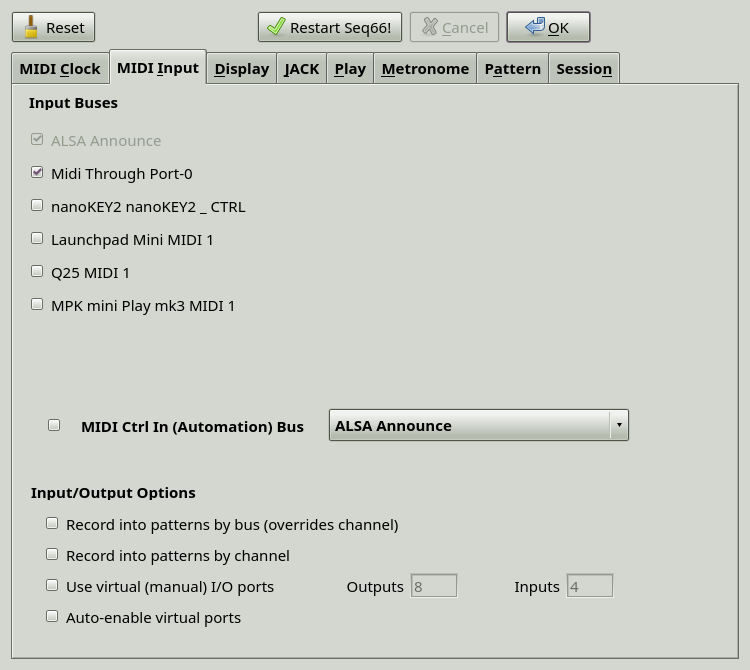
\includegraphics[scale=0.50]{main-menu/edit/preferences/midi_input_tab-2.png}
   \caption{MIDI Input Tab}
   \label{fig:midi_input_tab}
\end{figure}

   Port-mapping is the default, and when active, is shown in this pane.
   If there are more than about a dozen
   input ports in the system, then a vertical scrollbar appears.

   Any item checked allows \textsl{Seq66} to record MIDI from that source,
   which must be connected to this input port.

   \textbf{Warning:}
   \index{warnings!usr config}
   \index{usr config}
   If the 
   \texttt{[user-midi-bus-definitions]} value in the 'usr' configuration file
   is non-zero, and the
   corresponding number of
   \texttt{[user-midi-bus-N]} settings are provided, then
   the list of existing hardware will be ignored, and those values will be
   shown instead.
   This feature can be overridden with the
   \texttt{-{}-reveal-ports} (\texttt{-r}) option.
   If you define these sections, they should match your
   hardware exactly, and your hardware should not change from session to
   session (or port-mapping should be enabled).
   If the "auto ALSA ports" option is turned on, via the \texttt{-a} or
   \texttt{-{}-auto-ports} option, then
   the input ports from the system are shown.

   \setcounter{ItemCounter}{0}      % Reset the ItemCounter for this list.

   \itempar{Input Buses}{input buses}
   \textbf{Input Buses} delineates the MIDI input devices as noted above.

   \itempar{MIDI Control Input Bus}{midi control!input buss}
   \index{midi control!input}
   Use this control to select the input bus used for MIDI control automation of 
   application actions, loop actions, and mute-group actions.
   Requires a \textsl{reload session} to take effect.
   The number of the buss is stored in the 'ctrl' file named in
   \sectionref{paragraph:menu_edit_preferences_session},
   as the value of \texttt{control-buss}.
   If port mapping is enabled (now the default),
   the nick-name of the bus is stored instead of the number.

   \itempar{Input Options}{input options}
   \index{input options}
   \textbf{Input Options} adds further refinements to MIDI input.
   Currenty it has only one setting, for recording input into patterns by the
   channel in each event.

   \itempar{Record-by-Bus}{record!by bus}
   \index{input by buss}
   \textbf{Record into patterns by buss}
   causes MIDI input from multiple busses to be distributed to
   each sequence according to MIDI input buss number.

   \itempar{Record-by-Channel}{record!by channel}
   \index{input by channel}
   \textbf{Record into patterns by channel}
   causes MIDI input with multiple channels to be distributed to
   each sequence according to MIDI output channel number.

   Only one of these record-by options can be enabled at the same time.
   The record-by-buss option takes precedence.

   When these options are disabled,
   the normal recording behavior dumps all data into the current
   sequence, regardless of channel or buss.
   See \sectionref{sec:recording}, which describes recording in more detail.

   \itempar{Input/Output Virtual Ports}{ports!virtual}
   \textbf{Use virtual (manual) I/O ports}
   This option
   allows for configuration of the manual-ports option from within the
   user-interace. 
   Once the option is enable
   A \textsl{reload session} (see \sectionref{subsec:concepts_reload_session})
   is necessary for this option to take effect.

   \itempar{Virtual Ports Auto-Enable}{ports!virtual auto-enable}
   \textbf{Auto-enable virtual I/O ports}
   If set, the ports are all automatically enabled upon a restart.
   The following figure shows that a large number of virtual ports can be
   defined.

\begin{figure}[H]
   \centering 
   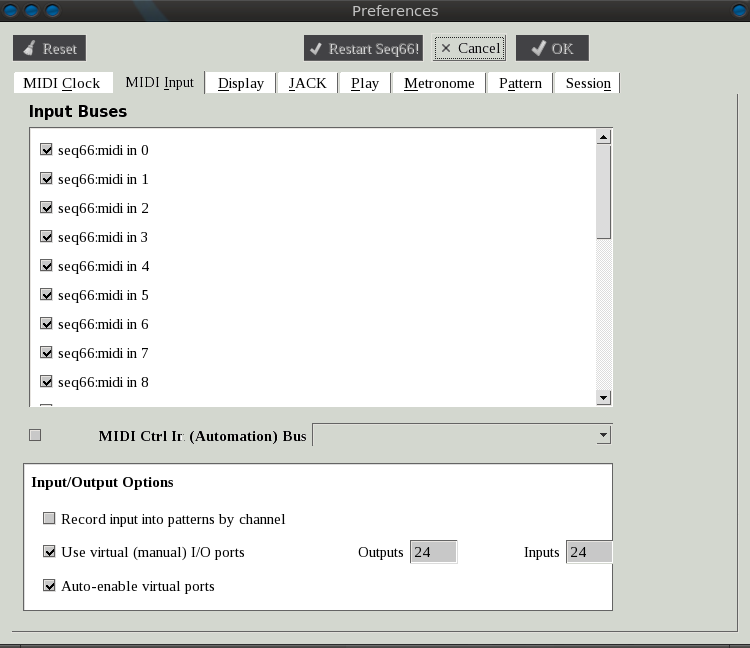
\includegraphics[scale=0.95]{main-menu/edit/preferences/midi_input_tab-virtual.png}
   \caption{MIDI Virtual Inputs}
   \label{fig:midi_input_tab_virtual}
\end{figure}

   Note that the user is responsible for connecting the virtual MIDI ports,
   using something like \textsl{aconnect} (ALSA) or
   \textsl{qjackctl} (JACK).

\paragraph{Menu / Edit / Preferences / Keyboard (removed)}
\label{paragraph:menu_edit_preferences_keyboard}

   Unlike \textsl{Seq24}, \textsl{Seq66}
   \textsl{does not} provide an options tab for
   setting up the keyboard.
   There are just too many new keystroke-automation functions to fit
   in a configuration dialog box.
   The default keyboard mappings follow \textsl{Seq24} fairly well,
   but add a large number of additional controls;
   around 96 keystroke slots would need to be provided!
   The keystroke and MIDI controls are consolidated, and are easy to change by
   editing the appropriate 'ctrl' configuration file, stored in one of the
   following directories, depending on
   the operating system:
   
   \begin{verbatim}
         /home/username/.config/seq66/qseq66.ctrl           (Linux)
         C:/Users/username/AppData/Local/seq66/qpseq66.ctrl (Windows)
   \end{verbatim}

   There are also some extended examples present in the \textsl{Seq66}
   \texttt{data/linux} and
   \texttt{data/samples} directory.
   Also see \sectionref{sec:launchpad_mini}.
   For more information on keystrokes, see
   \sectionref{subsec:kbd_mouse_keyboard_control}.

   One useful enhancement, though "costly", would be support of MIDI Learn.
   Currently the only "learnable" items are the mute groups.

\paragraph{Menu / Edit / Preferences / Mouse (removed)}
\label{paragraph:menu_edit_preferences_mouse}

   Unlike \textsl{Seq24}, \textsl{Seq66}
   \textsl{does not} provide an options tab for
   the mouse-interaction method.
   It is not supported in \textsl{Seq66}...
   the \textbf{Fruity} interaction method is not available;
   only the \textbf{Seq24} interaction is available.
 
\paragraph{Menu / Edit / Preferences / Display}
\label{paragraph:menu_edit_preferences_display}

   This dialog provides a few odds and ends to enhance the user-interface.
   Some of these items (plus a few more) can be configured by editing the 'usr'
   file.

\begin{figure}[H]
   \centering 
   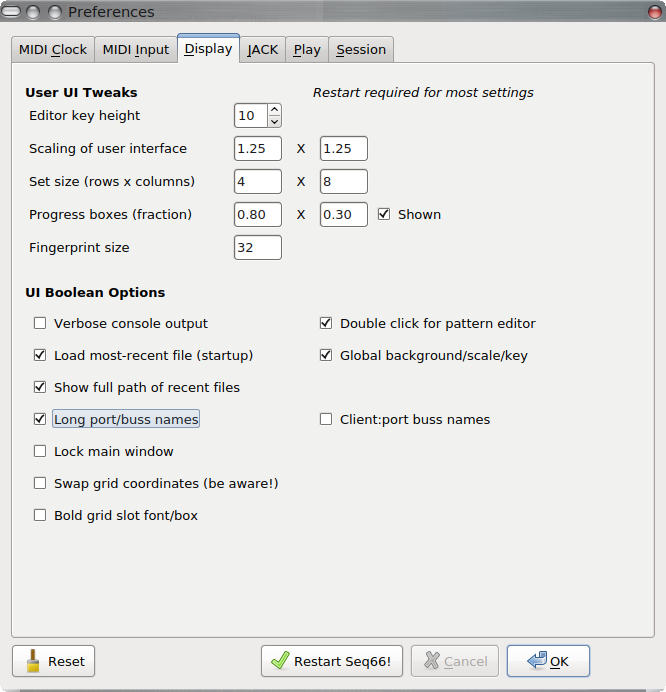
\includegraphics[scale=0.50]{main-menu/edit/preferences/midi_display_tab.png}
   \caption{Display Options}
   \label{fig:midi_display_tab}
\end{figure}

   \setcounter{ItemCounter}{0}      % Reset the ItemCounter for this list.

   \itempar{Editor Key Height}{key height}
   This option affects the pattern editor's piano roll.  Smaller means a wider
   range of notes can be shown.  There are also
   \textbf{-},
   \textbf{0}, and
   \textbf{+} buttons in the pattern editor that provide
   vertical zoom.

   \itempar{Grid scaling \& spacing}{window scaling}
   These three items set scale factor for width and height of the main window,
   and adjust the spacing between the grid slots..
   The lowest scale factor is 0.5, and the largest scale factor is 3.0.
   For the smallest window, the smallest practical values are 0.85 x 0.60.
   The spacing unit is pixels.

   \itempar{}{set-size}
   Provides a way to change the set size.  The default is
   \textbf{4 x 8}
   (rows by columns), but we intend to support
   \textbf{4 x 4},
   \textbf{8 x 8}, and
   \textbf{12 x 8}
   as well.

   \textbf{Warning}:
   A different set size alters the 'ctrl' file layout radically.
   We still have to work through all the implications of changing the set size,
   so back up your configuration and proceed with caution!

   \itempar{Progress Boxes}{progress-box size}
   Provides a way to change the size of the progress box in each button.
   Values are width and height fractions (up to 1.0) re the button size.
   This is a 'usr' option.

   \itempar{Progress Box Shown}{progress-box shown}
   If the \textbf{Shown} check-box
   is \textsl{unchecked}, then the progress boxes and pattern color are not
   shown.
   This is a 'usr' option.

   \itempar{Fingerprint Size}{fingerprint size}
   This value, if set from 32 to 128, indicates the number of events above
   which a "fingerprint", rather than every note, will be drawn.  It can
   save some CPU time in drawing the grid.  If set to 0, the whole
   pattern is drawn, no matter how long the pattern is.

   \itempar{Verbose Console Output}{verbose}
   This boolean makes more output appear if \textsl{Seq66} is run from a
   console/terminal. It will also increase the amount of data logged to the log
   file, if activated. It is only a temporary setting, just like
   its command-line counterpart, \texttt{--verbose}; when
   \textsl{Seq66} exits, the setting remains false.

   \itempar{Suppress startup error messages}{quiet}
   Unlike the verbose setting, this one is sticky.
   It prevents the display of error prompts at startup.
   It is useful when the system keeps flagging the same problem,
   it cannot be fixed, and can be ignored.
   It is \textsl{not} the opposite of "verbose".

   \itempar{Load Most Recent File (startup)}{load most-recent}
   If checked, the file at the top of the \texttt{[recent-files]}
   list in the 'rc' file is loaded at startup.

   \itempar{Show Full Path of Recent Files in Menu}{full paths}
   The full path of each file in the \texttt{[recent-files]} list
   is shown in the menu.  Although they can be uncomfortably long, they can
   show files that have the same name, but in different directores.

   \itempar{Long Port/Buss Name}{buss names!long}
   \index{buss names!short}
   Controls how much port information is shown in the clocks and input
   listings.  For the "portmidi" (e.g. \textsl{Windows})
   implementation, keep this option checked.

   \itempar{Lock Main Window}{main window!lock}
   This item makes the window non-resizable after startup.

   \itempar{Swap Coordinates}{grid!swap coordinates}
   Normally, \textsl{Seq66} displays the pattern and mute-groups grids
   where the pattern numbers increase fastest downward.
   Some might prefer to have pattern numbers increase fastest rightward.
   This setting make the patterns show in the more conventional manner.

   \textbf{Warning}:

      \begin{itemize}
         \item This setting requires the 'ctrl' file to be rewritten
            if one want to preserve the normal layout for the pattern hot-keys
            and the mute-group hot-keys.
         \item This setting has not been rigorously tested, so be prepared for
            some issues.
      \end{itemize}

   A 'ctrl' file for the swapped setting is provided
   in \texttt{qseq66-swapped.ctrl} in the \texttt{data/linux}
   directory, but it might not be completely correct yet.

   \itempar{Bold Slot Font}{grid!bold}
   \index{font!bold}
   \index{progress bar!thick}
   This setting makes the font in the live grid bold, and it allows
   make the progress-bar thick in the grid and in the Live and Song piano
   rolls.
   It is the same as the \texttt{progress-bar-thick = true} option in the 'usr'
   file. See \sectionref{subsubsec:usr_file_user_interface_settings}.

   \itempar{Double click for pattern editor}{grid!bold}
   \index{double-click!pattern slot}
   If set, a double-click on a grid button brings up the pattern for editing.
   Disable it if the effect is confusing.

   \itempar{Global background/scale/key}{globals!background etc.}
   \index{global pattern setting!background}
   \index{global pattern setting!key}
   \index{global pattern setting!scale}
   If set, setting the background sequence, scale to show, or the key of the
   track will apply to all pattern windows that are opened.

   \itempar{Client:port buss names}{buss!naming}
   \index{bus!naming}
   If checked the MIDI engine's "client:port" numbers are shown in the port
   listings.
 
\paragraph{Menu / Edit / Preferences / JACK}
\label{paragraph:menu_edit_preferences_jack}

   This tab sets up JACK transport, if \textsl{Seq66}
   was built with JACK support (\textsl{Linux} only).

\begin{figure}[H]
   \centering 
   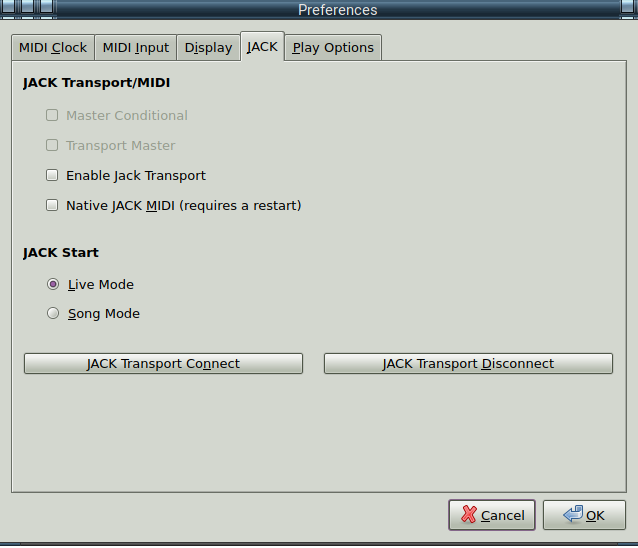
\includegraphics[scale=0.50]{main-menu/edit/preferences/midi_jack_tab.png}
   \caption{Edit / Preferences / JACK}
   \label{fig:midi_jack_tab}
\end{figure}

   The main sections in this dialog are:

   \begin{enumber}
      \item \textbf{JACK Transport/MIDI}
      \item \textbf{JACK Start Mode}
      \item \textbf{JACK Transport Connect and Disconnect}
      \item \textbf{JACK Server Settings}
   \end{enumber}

   \setcounter{ItemCounter}{0}      % Reset the ItemCounter for this list.

   \itempar{Transport/MIDI}{jack sync!transport/midi}
   These settings are stored in the 'rc' file settings group
   \texttt{[jack-transport]}.
   This items collects the following settings:

   \begin{itemize}
      \item \textbf{Jack Transport}.
         \index{JACK!transport}
         Enables slave synchronization with JACK Transport.
         The command-line option is \texttt{-{}-jack-transport}.
         The behavior of this mode of operation is perhaps not quite
         correct.  Even as a slave, \textsl{Seq66} can start and
         stop playback.
         Note that this option cannot be disabled via the mouse if the
         \textbf{Transport Master} option is enabled.  Disable that one first.
      \item \textbf{Transport Master}.
         \index{JACK!transport master}
         \textsl{Seq66} will attempt to serve as the JACK Master.
         The command-line option is \texttt{-{}-jack-master}.
         If this option is enabled the \textbf{JACK Transport} option is
         automatically enabled as well.
      \item \textbf{Master Conditional}.
         \index{JACK!master conditional}
         \textsl{Seq66} will fail to serve as the JACK Master if there is
         already a Master.
         The command-line option is \texttt{-{}-jack-master-cond}.
         If this option is enabled the \textbf{JACK Transport} option is
         automatically enabled as well.
      \item \textbf{Native JACK MIDI}.
         \index{JACK!native midi}
         This option is for the \texttt{qseq66} (Linux) version of
         \textsl{Seq66}.
         If set, MIDI input and output use native JACK MIDI,
         rather than ALSA.  However, if JACK is not running on the
         system, then \texttt{seq66} will fall back to ALSA mode.
         (However, if \texttt{jackdbus} is running, but the JACK engine is not,
         then a couple of non-working manual ports are created.  To be fixed in
         the future.)
         The command-line option is \texttt{-{}-jack-midi}
         or \texttt{-{}-jack}.
      \item \textbf{JACK Auto-Connect}.
         \index{JACK!auto-connect}
         This option has been true for a long time in \textsl{Seq66}, and
         non-configurable.  Now it can be turned off, in order to let the user
         or a session manager make the connections, even when not using
         manual/virtual ports.
   \end{itemize}

   \begin{quotation}
      \textbf{Tip}:
      Seq66 generally works better as JACK Master than JACK Slave.
   \end{quotation}

   If one makes a change in the JACK transport settings, it is best to
   then press the \textbf{JACK Transport Disconnect} button, then the
   \textbf{JACK Transport Connect} button.
   Another option is to restart
   \textsl{Seq66}... the settings are automatically saved when
   \textsl{Seq66} exits.

   \itempar{JACK Start mode}{jack sync!start mode}
   This item collects the following settings, also stored in the 'rc' file
   settings group \texttt{[jack-transport]}.

   \begin{itemize}
      \item \textbf{Live Mode}.
         \index{JACK!live mode}
         \index{live mode}
         \index{non-playback mode}
         Playback will be in live mode.  Use this option to allow muting and
         unmuting of patterns.  This option might also be called "non-song
         mode".
         The command-line option is \texttt{-{}-jack-start-mode 0}.
      \item \textbf{Song Mode}.
         \index{JACK!song mode}
         \index{song mode}
         \index{playback mode}
         \index{performance mode}
         Playback will use only the Song Editor's data.
         The command-line option is \texttt{-{}-jack-start-mode 1}.
   \end{itemize}

   \textsl{Seq66} also selects the playback modes
   according to which window started the playback.
   \textsl{The main window}, or pattern
   window, causes playback to be in live mode.  The user can arm and mute
   patterns in the main window by clicking on sequences, using their hot-keys,
   and by using the group-mode and learn-mode features.
   The song editor causes playback to be in performance mode, also known as
   "playback mode", or \textbf{Song} mode.

   \itempar{Connect}{jack sync!connect}
   Connect to JACK Sync.
   This button is useful to restart JACK sync when making changes to it,
   or when \textsl{Seq66} was started in ALSA mode.

   \itempar{Disconnect}{jack sync!disconnect}
   Disconnect from JACK Sync.
   This button is useful to stop JACK sync when making changes to it.
   JACK connection and disconnection are disabled during playback, but the
   buttons don't yet reflect that status.

   \itempar{JACK Server Settings}{jack server!settings}
   This read-only section shows the current settings of the JACK
   server, as much as possible.

\paragraph{Menu / Edit / Preferences / Play Options}
\label{paragraph:menu_edit_preferences_play_options}

   This tab contains some disparate options ostensibly related to playback.

\begin{figure}[H]
   \centering 
   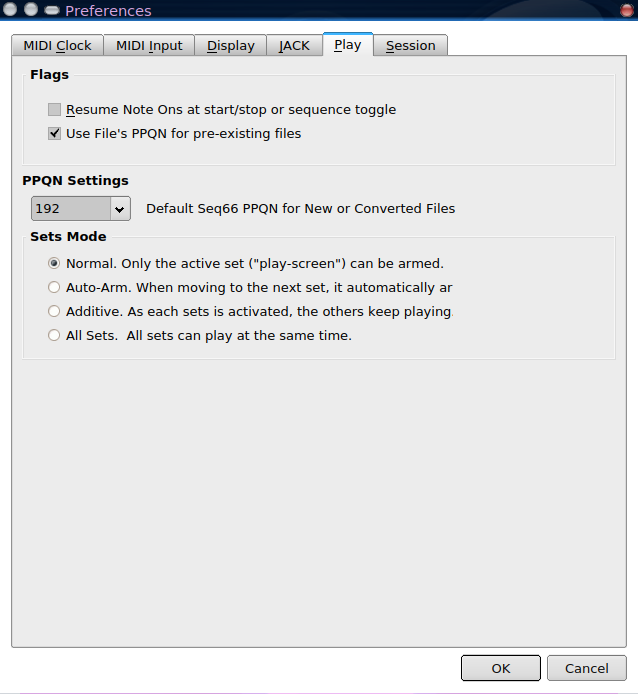
\includegraphics[scale=0.50]{main-menu/edit/preferences/midi_play_options_tab.png}
   \caption{Play Options}
   \label{fig:midi_play_options_tab}
\end{figure}

   \setcounter{ItemCounter}{0}      % Reset the ItemCounter for this list.

   \itempar{Resume Note Ons...}{edit!resume notes}
   \textbf{Resume Note Ons at start/stop or sequence toggle}
   allows notes that had already started
   to be resumed when playback resumes.

   \itempar{Use File's PPQN...}{edit!use file ppqn}
   \textbf{Use File's PPQN for Pre-Existing Files}, if checked, allows
   \textsl{Seq66} to run using the PPQn of the MIDI file rather than
   the default \textsl{Seq66} internal PPQN.
   This is the recommended option for most MIDI files.
   When this option is changed, the \texttt{-{}-user-save} option is turned on
   to preserve the setting when \textsl{Seq66} exits.

   \itempar{Default Seq66 PPQN...}{edit!default ppqn}
   \textbf{Default Seq66 PPQN for New or Converted Files}, if checked, allows
   the standard PPQN, 192 pulses/quarter-note, to be changed to discrete values
   from 32 to 19200.  Intermediate values, even oddball values, can be entered
   by typing the number directly.
   When this option is changed, the \texttt{-{}-user-save} option is turned on
   to preserve the setting when \textsl{Seq66} exits.
   If there is a MIDI file loaded, it is modified to use the new PPQN, and the
   user is prompted to save it at exit.
   Best to have a backup, just in case.

   \itempar{Sets Mode}{edit!sets-mode}
   This item determines how sets are handled.
   Recall that a set is a number of patterns (up to 4x8) in the pattern grid,
   and that the current set is the one visible in the pattern grid.
   The way sets work in \textsl{Seq66} is that, when a set is selected,
   all the patterns in it are loaded into what is called
   the "play-set".
   When play starts only, patterns in the play-set are handled.
   The \textbf{Sets Mode} option allows special handling of the play-set.

   \begin{enumerate}
      \item \textbf{Normal}.
         In this mode, only the current set's patterns can be unmuted.
         When switching to another set, the current set's patterns become
         muted, and the new set's patterns are shown, unmuted.
      \item \textbf{Auto-Arm}.
         Here, when the new set is loaded, it is immediately unmuted.
      \item \textbf{Additive}.
         With this option, when a new set is loaded, the previous set keeps
         playing. This allows a build-up of patterns in playback.
      \item \textbf{All Sets}.
         Here, all sets in the tune are loaded and unmuted at once.
         Try this mode with the \texttt{b4uacuse-stress.midi} file
         in the \textsl{Sequencer64} project.  It's a good test of
         \textsl{Seq66} and your hardware/software synthesizer!
   \end{enumerate}

   One can clear the out play-set, and set only the current set active, by
   clicking the exclamation point button to the left of the "Active" label at
   the bottom of the main windows.

\paragraph{Menu / Edit / Preferences / Metronome Options}
\label{paragraph:menu_edit_preferences_metronom_options}

   This tab contains options for the "metronome" and
   "background recording" features:

\begin{figure}[H]
   \centering 
   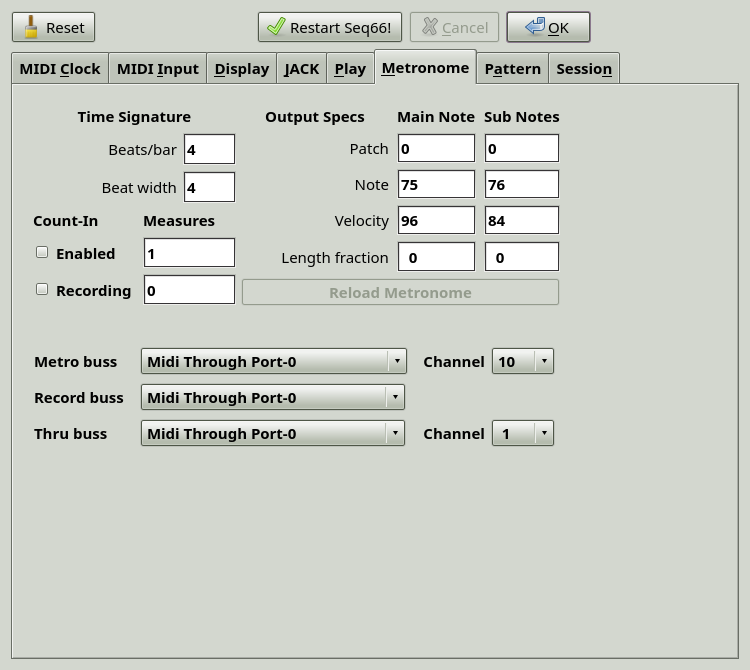
\includegraphics[scale=0.50]{main-menu/edit/preferences/midi_metro_options_tab.png}
   \caption{Metronome Options}
   \label{fig:midi_metro_options_tab}
\end{figure}

   \setcounter{ItemCounter}{0}      % Reset the ItemCounter for this list.

   The metronome feature is enabled in the main live grid via a metronome
   button.
   The metronome is a standard \textsl{Seq66} pattern that is used
   for playback of the metronome, but it is never seen
   nor directly edited by the user.
   It is not saved with a song, so changing the metronome does not modify the
   song.
   The settings shown above are saved to a "metronome" section in the 'rc'
   file.
   The metronome is a pattern that first plays a main note once, and then
   plays "sub" notes for the rest of the measure.
   Here are the settings:

   \itempar{Beats/bar}{metronome!beats/bar}
   This setting sets the beats-per-measure for the metronome only.
   It currently does not affect the time-bar in the main window.
   Should it? There is a global beats/bar as well as beats/bar for
   each pattern.

   \itempar{Beat width}{metronome!beat width}
   This setting sets the beat width for the metronome only.
   The following settings are provided for the "main" note
   (the note that occurs on the beginning of the measure)
   and the "sub" notes (the notes that occur on each beat):

   \itempar{Patch}{metronome!patch}
   This item sets the program (patch) number for the note, which sets the
   instrument to play for the notes.
   We currently do not have a drop-down box to select the patch by name.
   The default patch is 0.
   As noted below, the default channel is 10, so this
   patch is the "Standard Drum Kit" for the device.
   Thus, by default the metronome can be implemented by two different
   drums.

   \itempar{Note}{metronome!note}
   This item provides the note value to be played.  Recall that 60 is the same
   as "middle C".  By default, the main note is 75, the "Clave" for the drum
   kit, and the sub note is 76, the "High Wood Block" for the drum kit.

   \itempar{Velocity}{metronome!velocity}
   This item provides the note velocity to be played, to provide an accent on
   the main note.

   \itempar{Length Fraction}{metronome!length fraction}
   The length of the notes are specified as a fraction of the beat width, and
   this value ranges from 0.125 to 1.0 to 2.0.
   If set to 0, the length is half of the beat width.

   \itempar{Reload Metronome}{metronome!reload}
   This button pauses playback (if playing),
   loads in the new metronome settings, and
   continues playing (if it was playing).
   It is \textsl{not} enabled when the status/configuration of background
   recording changes.

   \itempar{Metro Buss}{metronome!buss}
   This value selects the output MIDI device to use to play the metronome.
   It \textsl{must} be enabled in the \textbf{MIDI Clock} list.

   \itempar{Channel}{metronome!channel}
   This value selects the channel to use to play the metronome.

   \itempar{Record Buss}{recorder!buss}
   \index{background recorder}
   This value selects the input device to use to record events into the
   background pattern.
   Note that this device \textsl{must be enabled} in the \textbf{MIDI Input}
   buss list.

   \itempar{Thru Buss}{record!thru buss}
   This value selects the output MIDI device to use to play the incoming
   background record notes.  Otherwise they will not be heard.
   It \textsl{must} be enabled in the \textbf{MIDI Clock} list.

   \itempar{Thru Channel}{recorder!thru channel}
   This value selects the channel to use to play the recorded notes as
   they come in.

   We still have some more work to do to refine the metronome, the
   background recorder, and their configuration, pending user input.
   For more information about the metronome, see
   \sectionref{paragraph:patterns_metronome}.
   For information on count-in background recording, see
   \sectionref{paragraph:patterns_background_recording}.

\paragraph{Menu / Edit / Preferences / Pattern}
\label{paragraph:menu_edit_preferences_pattern}

   This tab provides options for the status of newly-created patterns
   and for randomization of amplitude and jitter of time-stamps.

\begin{figure}[H]
   \centering 
   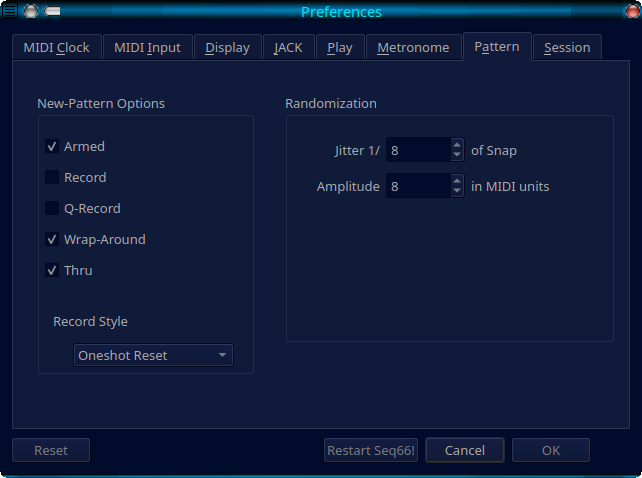
\includegraphics[scale=0.50]{main-menu/edit/preferences/midi_pattern_tab.png}
   \caption{Pattern Options}
   \label{fig:midi_pattern_options_tab}
\end{figure}

   \itempar{Pattern}{edit!pattern}
   \textbf{Pattern}
   This relatively new tab provides a way to configure the status of
   a newly-created pattern.
   It also provides a way to change the range of amplitude randomization
   and time jittering of events.

   The first section is \textbf{Pattern Options}.
   It defines the statuses of a newly-created or newly-opened pattern.
   This can be convenient for live-recording.
   The status setting are:

   \begin{itemize}
      \item \textbf{Armed}.
         This setting causes the pattern to be armed when a new pattern
         is created.
      \item \textbf{Record}.
         The new pattern starts in record mode.
      \item \textbf{Tighten record}.
         The new pattern starts in tightened (partly quantized) record mode.
      \item \textbf{Quantize record}.
         The new pattern starts in quantized record mode.
      \item \textbf{Note-map record}.
         The new pattern starts in note-mapping record mode.
         Notes are translated live via a 'drums' file, if set active
         in the 'rc' file.
      \item \textbf{Wrap-around}.
         The new pattern will allow prolonged notes to wrap around so
         that the Note Off event precedes the Note On event in the
         pattern loop.
      \item \textbf{MIDI Thru}.
         The new pattern starts with MIDI Thru enabled.
      \item \textbf{Apply only to new}.
         If check-marked, then the settings are applied only to
         newly-created patterns. Often one might not want to
         automatically record into an existing pattern, for example.
      \item \textbf{Record Style}
         This setting sets how record mode works for the pattern.
         \begin{itemize}
            \item \textbf{Merge}.
               As recording and looping proceeds, new events merge with
               the existing events.
            \item \textbf{Overwrite}.
               When the pattern loops back to its beginning, any
               existing events are deleted.
               A good way to try to get the right collection of notes.
            \item \textbf{Expand}.
               When recording as notes are recorded, the pattern expands to
               accomodate them.
               This results in a longer pattern than initially specified.
            \item \textbf{Oneshot}.
               Events are entered until the end is reached.
               Useful for recording stock patterns from a drum machine.
            \item \textbf{Oneshot Reset}.
               At the end of the specified length of the pattern,
               all events are cleared.
               Normal recording is set.
               Need to look into this as we cannot rememember all the
               details :-D.
         \end{itemize}
      \item \textbf{Apply to new only}.
         If checked, only a newly-created pattern will have the options
         above automatically applied.
   \end{itemize}

   The second section is \textbf{Randomization}.
   The range of randomization is based on a range parameter, and
   goes from -range to +range.
   The concept of jitter means that the time-stamps of recorded events
   are randomized slightly.
   The concept of randomization means that the amplitudes of events
   are randomized slightly.
   The randomization settings are:

   \begin{itemize}
      \item \textbf{Jitter}.
         This value is a jitter divisor.
         It sets the fraction of of the current snap value that
         is used as the range of jittering the time.
         For example, "8" means that the range is 1/8th of the snap value.
      \item \textbf{Amplitude}.
         This value is used for various data values.
         For Notes On (but not Notes Off), this parameter affects
         the range of amplitude variation, when amplitudes are
         the standard MIDI range, 0 to 127.
   \end{itemize}

   One minor issue, which we're still trying to work around, is that
   our various randomization algorithms seem biased to emit
   negative numbers.
   If one clicks in a pattern editor piano roll, types
   \texttt{Ctrl-A} to select all notes (and aftertouch)
   and types the \texttt{r} key repeatedly to randomize
   note amplitudes, the overall velocities slowly descend to 0.
   Still not sure what's wrong with \textsl{Seq66} randomization, 
   but it is only important if randomizing a large number of times.

   The next section is \textbf{Additional 'usr' Options}.
   It contains only one option at present,
   \textbf{Esc key in piano roll closes external editor}.
   If set (the default is false), then the \texttt{Esc}
   key can not only stop playing and exit paint mode, but
   can also close the pattern window.
   Be careful. It's your call.

\paragraph{Menu / Edit / Preferences / Session}
\label{paragraph:menu_edit_preferences_session}

   This tab contains options related to session management and the
   configuration files.

   \setcounter{ItemCounter}{0}      % Reset the ItemCounter for this list.

\begin{figure}[H]
   \centering 
   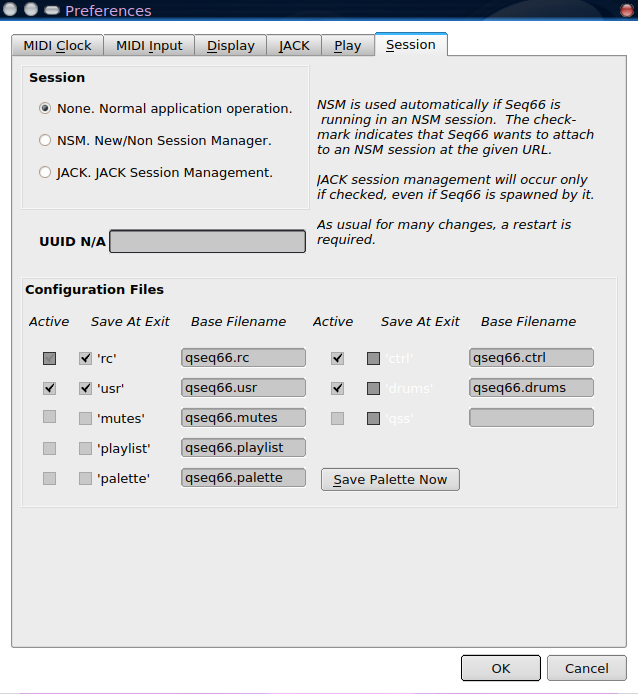
\includegraphics[scale=0.50]{main-menu/edit/preferences/midi_session_tab.png}
   \caption{Session Options}
   \label{fig:midi_session_options_tab}
\end{figure}

   This dialog has a couple of new items, to allow changing the web browser and
   PDF view to use.  See below.

   \setcounter{ItemCounter}{0}      % Reset the ItemCounter for this list.

   \itempar{Session}{edit!session}
   \textbf{Session}
   This tab provides for three modes of session management:  None, the
   Non/New Session Manager (NSM), and JACK Session management.
   None is the normal mode of operation, where the user has full control of
   where to put files, what other applications are to be run alongside
   \textsl{Seq66}, and what connections are to be made.

   NSM provides a rigorously-controlled session management, and directs
   \textsl{Seq66} what menu items to display, whether to hide the
   user-interface or not, where configuration files and MIDI files go, and what
   applications are run in a session. It can also (via \texttt{jackpatch}) keep
   a record of connections to reconstruct.

   JACK Session provides a location for file and a record of applications and
   connections, but otherwise lets the user mess things up.  It is
   provided because some people still use it.
   For more information about session management, see
   \sectionref{sec:sessions}.

   \itempar{UUID}{edit!UUID}
   \textbf{UUID} is a read-only field that shows any UUID that's relevant to a
   session. Normally has a value only in a \textsl{JACK} or
   \textsl{NSM} session.
   Also see the \textbf{Session} tab in the main window
   (\sectionref{sec:sessions}).

   \itempar{Configuration Files}{edit!configuration}
   \textbf{Configuration Files}
   shows the status of the configuration files.
   (See \sectionref{subsec:configuration_rc}).
   The 'rc' file is always active, and normally is saved at exit (even if no
   configuration changes occurred).

   The 'usr' file should also be active, but one can disable it, which is
   currently an \textsl{experimental} and \textsl{untested} option.
   Normally, it is not saved at application exit (except after the first run on
   one's system).
   (See \sectionref{subsec:configuration_usr}).

   The rest of the configuration files are optional.
   See
   \sectionref{subsec:configuration_ctrl},
   \sectionref{subsubsec:configuration_mute_group_control},
   \sectionref{subsec:configuration_drums}, and
   \sectionref{sec:playlist}.

   \itempar{Palette File Base Name}{palette}
   This text edit holds the base name of a 'palette' file, which is always
   stored in the \textsl{Seq66} configuration directory.
   (See \sectionref{sec:palettes}.)

   \itempar{Store Palette}{palette}
   Normally, there is no palette file.  Pushing this button creates one, which
   can then be modified and configured as the palette-file to use in the 'rc'
   file.

   \itempar{Browser}{browser}
   This field is text-editable, and can also be changed by using the button
   next to it to select a browser executable to use in the
   \textbf{Help / Tutorial} menu entry. If all possible browsers are available
   via one's \texttt{PATH}, then the simple name of the application
   (including \texttt{.exe} if running \textsl{Windows}) can simply be typed
   in. Otherwise, type in the complete path or use the button to bring up
   a file dialog.

   If one erases the file name, the default browser for the system will be
   used the next time \textsl{Seq66} is restarted.

   \itempar{PDF Viewer}{PDF viewer}
   This field is similar to the browser field, but specifies an alternate
   viewing application for PDFs.

\subsection{Menu / Help}
\label{subsec:menu_help}

   The usual \textbf{Help} dialog is provided.
   As of version 0.98.8, it has been beefed up with a way to access a
   tutorial and the user manual.

   These new help items are a work in progress, so please apprise
   us of any issues; include information on the operating system and,
   if \textsl{Linux}, the desktop/window manager in use.

\subsubsection{Menu / Help / About...}
\label{subsubsec:menu_help_about}

   \index{Help!about}
   This menu entry shows the "About" dialog.
   That dialog provides access to some credits for the program as well.
   authors and the project documentors, and active link to them.
   It also shows Git version-control information as well.

\subsubsection{Menu / Help / Build Info...}
\label{subsubsec:menu_help_build_info}

   \index{Help!build info}
   This menu entry shows the "Build Info" dialog.  This list of
   build options enabled in the current application is the same list
   that it generated via this command line:

   \begin{verbatim}
      $ seq66 --version
   \end{verbatim}

\subsubsection{Menu / Help / Song Summary File...}
\label{subsubsec:menu_help_song_summary_file}

   \index{Help!song summary}
   This menu entry allows one to write a summary of the song data into a text
   file. It brings up a file dialog which defaults to the name of the
   currently-loaded MIDI file, with the extenstion \texttt{.text} and
   the directory from where the MIDI file was loaded.
   It shows the filename, the information about the sets and tracks,
   MIDI format (0 or 1), and the PPQN.

   It also shows each sequence: name, channel (128 mean there is no output
   channel), the time signature, buss number (and any mapping), the length in
   pulses, the event and trigger count, transposability, key and scale, and
   color number (if any).
   For each trigger in the pattern, its start, stop, offset, and transposition
   values are shown.
   This file can be helpful for trouble-shooting or solving puzzling effects in
   the tune.

\subsubsection{Menu / Help / App Keys}
\label{subsubsec:menu_help_app_keys}

   \index{Help!app keys}
   This entry brings up a dialog that shows brief descriptions of the
   non-automation keys available in various contexts.
   These keys are almost exclusively hardwired and currently cannot be
   changed via a configuration file.  By pressing a button, the desired
   keystrokes can be quickly viewed. Note that the descriptions come from small
   HTML files that are part of the installation.

\subsubsection{Menu / Help / Tutorial}
\label{subsubsec:menu_help_tutorial}

   \index{Help!tutorial}
   This entry brings up a short tutorial of \textsl{Seq66} in the default
   browser. This tutorial is meant only to jump-start a new user of
   \textsl{Seq66}, and is a work in progress.
   It does not cover nearly as much as the user manual, so check that out in
   the next section.

   Normally, the tutorial will open a web page.  If it does not, one might need
   to set up a default browser.  On Linux, make sure that there is a "desktop"
   file for the browser, as in
   \texttt{/usr/share/applications/firefox.desktop}.
   If so, then run the following command, and then test it:

   \begin{verbatim}
      $ xdg-settings set default-web-browser firefox.desktop
      $ xdg-open https://ahlstromcj.github.io/docs/seq66/tutorial/index.html 
   \end{verbatim}

   On Windows, this procedure is still \textsl{to be determined}.

   In both systems, one can override the default applications by opening
   the specified 'usr' file (usually \texttt{qseq66.usr} or
   \texttt{qpseq66.usr} and specifying the full path to the desired
   applications (Linux paths shown here):

   \begin{verbatim}
      [user-options]
      log = "/home/user/.config/seq66/seq66.log"
      pdf-viewer = "/usr/bin/zathura"
      browser = "/usr/bin/google-chrome"
   \end{verbatim}

   Also see \sectionref{subsubsec:usr_file_user_options}.

\subsubsection{Menu / Help / User Manual}
\label{subsubsec:menu_help_user_manual}

   \index{Help!user manual}
   This menu entry first tries to locate the user manual on the internet and
   open it in the default browser. If not found, or the network is down,
   then this entry brings up the full \textsl{Seq66} user manual in the default
   PDF viewer.  It currently looks in the possible installation areas and in
   the \textsl{Seq66} source tree to find the PDF.

   On Linux, one can follow the setup procedure in the previous section and
   test it via the following command, which will show the manual in the default
   browser.:

   \begin{verbatim}
      $ xdg-open https://ahlstromcj.github.io/docs/seq66/seq66-user-manual.pdf
   \end{verbatim}

%-------------------------------------------------------------------------------
% vim: ts=3 sw=3 et ft=tex
%-------------------------------------------------------------------------------


% Patterns Panel

%-------------------------------------------------------------------------------
% patterns_panel
%-------------------------------------------------------------------------------
%
% \file        patterns_panel.tex
% \library     Documents
% \author      Chris Ahlstrom
% \date        2015-08-31
% \update      2023-09-20
% \version     $Revision$
% \license     $XPC_GPL_LICENSE$
%
%     Provides the concepts.
%
%-------------------------------------------------------------------------------

\section{Patterns Panel}
\label{sec:patterns_panel}

   \textsl{Seq66} works with patterns (also known as "loops", "tracks", or
   "sequences") that are repeated throughout a song.
   One composes and edits small patterns in a grid,
   and combines them to create a full song.
   This is a powerful way to work, and makes one productive quickly.

   \index{Patterns Panel}
   \index{Live Frame}
   \index{Live Grid}
   The \textbf{Patterns Panel}, also called the
   \textbf{Live Frame} or
   \textbf{Live Grid} or
   is in the center of the
   \index{main window}
   \textbf{main window} of \textsl{Seq66}.
   See \figureref{fig:main_screen_annotated}.
   It is here one creates a set of patterns ("screenset"),
   manages the configuration, controls the playback rate, adds tempo events,
   and opens the pattern, song, event, mute-groups, or playlist editors.

   The musician can
   control the playback and muting/unmuting of each pattern in
   the song, while it is playing, from within this window.
   One can also switch to other screensets, to work with a different
   part of the song.

   For exposition, we divide the patterns panel
   into a menu bar, a top panel, a pattern panel (live frame/grid),
   and a bottom panel.
   The \textsl{Seq66} menu bar is discussed in \sectionref{sec:menu}.

\subsection{Patterns / Main Panel}
\label{subsec:patterns_panel_main}

   The main panel of the application provides a grid of empty boxes,
   as shown in
   \figureref{fig:patterns_panel_popup_menu}.
   Each filled box represents a loop, track, sequence, or pattern
   (interchangeable terms).
   One sees only 32 loops at a time in the main panel (but many more than
   32 loops can be supported by \textsl{Seq66}).

   \index{screen-set}
   This group of 32 loops is called a "screen-set".
   One can switch between sets by using the
   \index{keys![}
   \index{keys!screenset down}
   "\texttt{[}" and
   \index{keys!]}
   \index{keys!screenset up}
   "\texttt{]}" keys on the keyboard, or by using
   the spin-widget-driven, labelled \textbf{Set} interface item, or
   \index{keys!Home}
   \index{keys!screenset play}
   by hitting the (default) \texttt{Home} key to make it the playing screenset,
   or by hitting \texttt{Page-Up} or \texttt{Page-Down} with the pattern window
   in keyboard focus.
   There are a total of 32 sets, for a total of 1024 loops/patterns. 
   Only one screen-set can be controlled at a time, in general.
   Multiple screensets can be playing at the same time, depending on
   configuration.

   The \texttt{Page Up} and \texttt{Page Down}, and \texttt{Up/Down Arrow}
   keystrokes can be used inside of the \textbf{Set} spin-button.
   It is important to note that, currently, incrementing or decrementing
   the screen-set will \textsl{not} wrap-around.
   We consider this a feature rather than a bug, at this time.
   There are some other important considerations for set-handling.
   See \sectionref{sec:setmaster}.

\begin{figure}[H]
   \centering 
   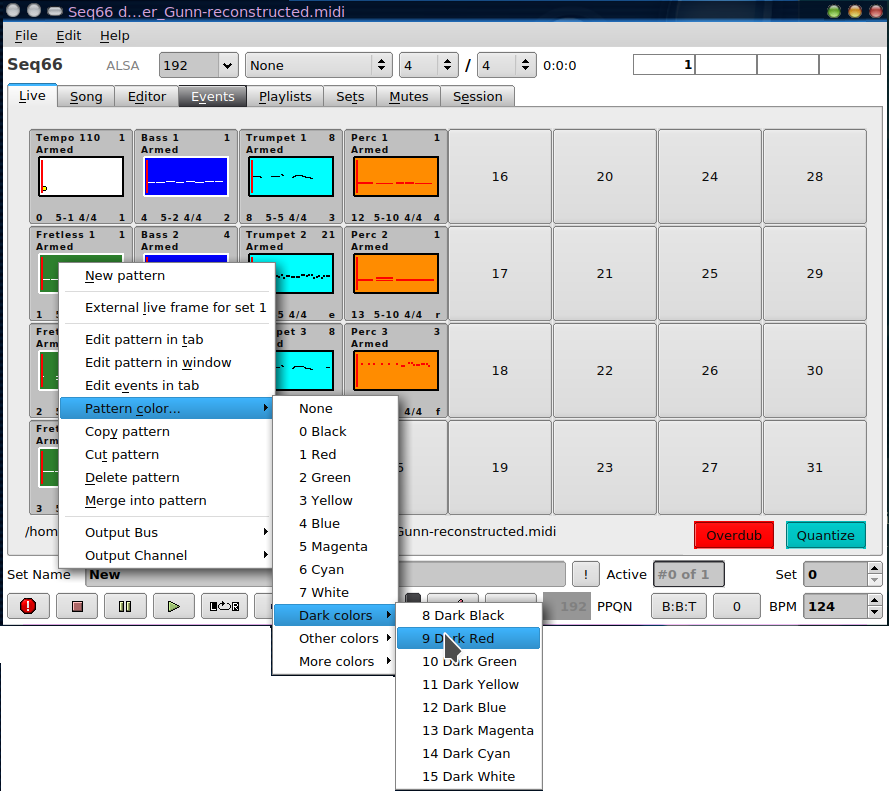
\includegraphics[scale=0.75]{tabs/live/pattern-popup-menu.png}
   \caption{Patterns Panel Pop-up Menu}
   \label{fig:patterns_panel_popup_menu}
\end{figure}

   The individual items annoted in this figure are described in
   \sectionref{subsubsec:patterns_pattern_filled}, in more detail.
   This figure is a little out-of-date re version 0.99.9.
   Also note the buttons for changing and showing the
   loop/recording modes of the grid buttons and recording quantization.
   \textsl{Seq66}'s pattern grid can be put in various recording
   modes (e.g. overdub/merge versus overwrite) where, instead of
   muting/unmuting the patterns, it turns on recording (without opening the
   pattern editor).
   Quantization can be turned on globally in \textsl{Seq66}'s pattern grid
   as well.
   These operations are also available as automation controls.
   See \sectionref{paragraph:configuration_midi_record_quan}.

   Observe that feature in the first figure of the next section.
   The two main items are the empty \textsl{pattern slot}, and the slot filled
   with a MIDI \textsl{pattern}:

   \begin{enumber}
      \item \textbf{Pattern Slot}
      \item \textbf{Pattern}
   \end{enumber}

\subsubsection{Pattern Slot}
\label{subsubsec:patterns_pattern_slot}

   \index{pattern!slot}
   An empty box is a slot for a pattern.
   If a pattern is present in the slot, text information and notes are drawn on
   the button.
   The top line will show
   the title of the pattern, the number of measures in the pattern, and
   indicate if the pattern has a loop-count (indicated by a
   \textbf{+} sign.
   A \textsl{right-click} over a pattern button brings up a fairly extensive
   popup menu.
   Also see \sectionref{subsubsec:patterns_pattern_filled}.

%  The slot at the bottom left of this figure shows the features:
%
%  \begin{itemize}
%     \item The sequence number (from 0 on up) appears at the bottom left of
%        the slot.
%     \item The buss number (re 0) and the channel number (re 1) appears
%        to the right of the sequence number, in the format "0-1".
%     \item To the right of that, the time signature ("4/4") appears, at the
%        bottom.
%     \item The hot-key for muting/unmuting the pattern appears next,
%        at the bottom right of the slot.
%     \item The title of the sequence appears at the top left of the pattern
%        slot.
%     \item The length of the sequence, in number of measures (bars), appears
%        at the upper right of the slot.
%     \item The font is a \textsl{Qt} font.
%  \end{itemize}

   A pattern can show a number of different statuses based on the coloring
   of elements in the pattern slot.
   (However, note that some of the special coloring using in
   \textsl{Sequencer64} is not supported in \textsl{Seq66}.

   \begin{itemize}
      \item \textbf{Empty background}.
         When the default button coloring for
         the current \textsl{Qt} theme is shown, without a pattern box,
         this state indicates that the slot is unused.
      \item \textbf{Yellow pattern box}.
         This color is used when a pattern is
         first created by \textsl{double-clicking} on the slot.
         However, this color sticks even when notes are added.
         Feel free to change it to another color, or no color.
      \item \textbf{Normal background}.
         Unarmed (muted) patterns show the
         unactivated/unchecked state of the button as per the \textsl{Qt}
         theme.  If a color is applied, it has a slight bit of alpha in the
         color so that the color appears muted.
      \item \textbf{Active background}.
         An armed (unmuted) pattern shows the
         activated/checked state of the button as per the \textsl{Qt}
         theme.  If a color is applied, it has no transparency, and the 
         color appears bright.
      \item \textbf{Line events}.
         \index{event!note}
         Lines indicate the presence of notes.  Depending on settings, the
         lines indicate the notes themselves, or a "fingerprint", a condensed
         indication of notes useful in reducing the overhead of
         drawing long patterns.
      \item \textbf{Red events}.
         \index{event!drum note}
         Indicates a pattern for which the transpose feature is
         disabled.  Most useful with drum patterns.
      \item \textbf{Circular events}.
         \index{event!tempo}
         Small circles indicate tempo events.  Generally, these events should
         appear only in the tempo track (which is normally track 0).
   \end{itemize}

   The user can also apply coloring to each sequence.
   This feature was adopted from \textsl{Kepler34} \cite{kepler34}.
   The color is more saturated when the pattern is unmuted.
   \index{pattern!color menu}

   \index{pattern!right click}
   \index{slot!empty slot right-click}
   \textsl{Right-clicking} on an empty box one brings up a menu to create
   a new loop or open an external live grid, as well as some other operations.

   \begin{enumber}
      \item \textbf{New pattern}
      \item \textbf{External live frame for set 0}
   \end{enumber}

   \setcounter{ItemCounter}{0}      % Reset the ItemCounter for this list.

   \itempar{New}{pattern!new}
   Creates a new loop or pattern.
   Clicking this menu entry fills in the empty box with an untitled
   pattern.
   Another way to create a new loop (without using the menu), is
   to hold the \texttt{Ctrl} key and click on the slot.
   A third to create a new loop is to
   \textsl{double-left-click} on an
   empty slot; this also brings up an external pattern editor (discussed
   later).

   \itempar{External live frame for set 0}{live!external}
   This option brings up an external \textbf{Live} frame window, which
   is the same as the patterns panel, but can be used to show a different set
   in a multi-set project.  Up to 32 external live frames can be shown.
   An external live grid can be activated by the \textbf{Activate} button,
   which sets the playing screen-set
   (and updates the main window to match).
   Another way to bring up an external live frame
   is to hold the \texttt{Shift} key and click on the slot.

\begin{figure}[H]
   \centering 
   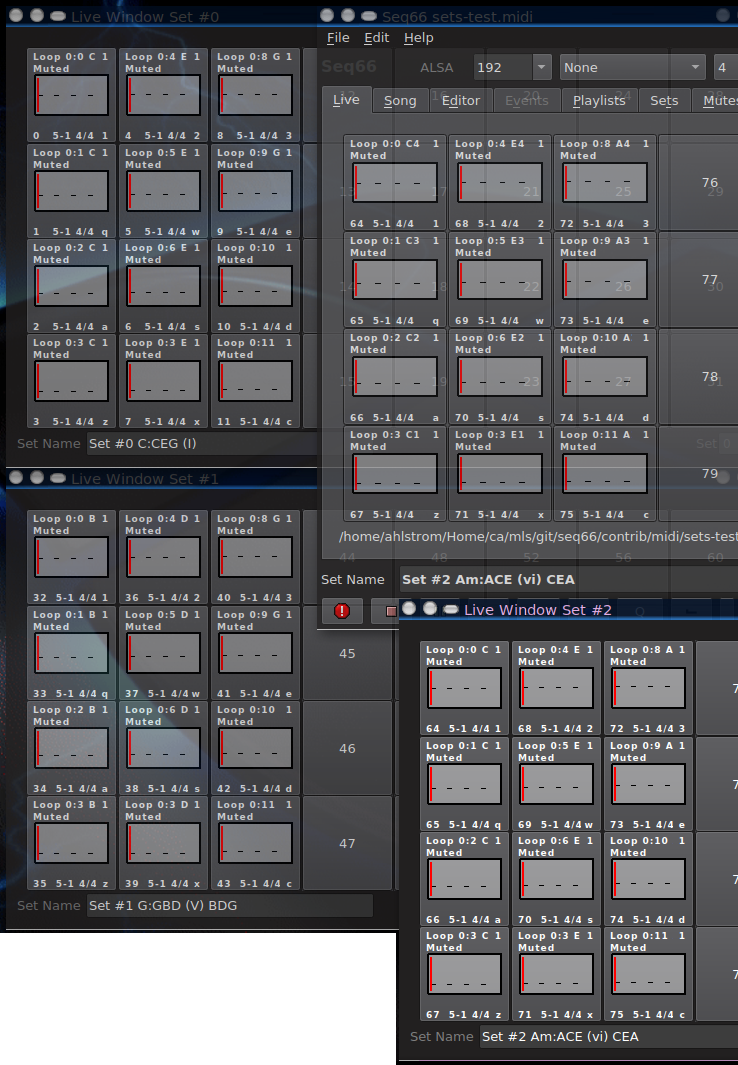
\includegraphics[scale=0.65]{main-window/multiple-live-grids.png}
   \caption{Multiple Live Grids}
   \label{fig:multiple_live_grids}
\end{figure}

   Note that the right-click slot menu has some items removed when the live
   grid is in an external window, or the main window is showing a set other
   than set 0, as indicated by
   the asterisks in the list below.
   \textsl{We hope to rectify that in a future release.}

   Once a new loop is created, there are more options for that slot.
   \index{pattern!right click}
   A \textsl{right-click} on an already-filled box brings up a menu
   to allow one to edit it, or perform a few other actions
   specified in the context menu.  Here is that menu:

\begin{figure}[H]
   \centering 
   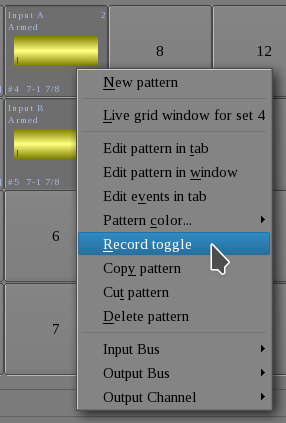
\includegraphics[scale=0.65]{main-window/slot-record-toggle.png}
   \caption{Slot Popup Menu (as of 0.99.9)}
   \label{fig:slot_record_toggle}
\end{figure}

   \begin{enumber}
      \item \textbf{New pattern}
      \item \textbf{External live frame for set ...} *
      \item \textbf{Edit pattern in tab} *
      \item \textbf{Edit pattern in window} *
      \item \textbf{Edit events in tab} *
      \item \textbf{Pattern color}
      \item \textbf{Record toggle} (new)
      \item \textbf{Copy pattern}
      \item \textbf{Cut pattern}
      \item \textbf{Delete pattern}
      \item \textbf{Merge into pattern}
      \item \textbf{Input Bus} (new)
      \item \textbf{Output Bus}
      \item \textbf{Output Channel}
   \end{enumber}

   The first menu entry is the same as above.  However, since there is
   already a pattern present in the slot, the user is prompted before erasing
   the current pattern and creating a new one.

   \setcounter{ItemCounter}{0}      % Reset the ItemCounter for this list.

   \itempar{New Pattern}{pattern!new}
   Creates a new pattern in the empty slot.
   \index{slot!double-click}
   Can also be done by double-clicking on an empty slot.

   \itempar{External Live Frame for Set}{pattern!external live frame}
   This selection uses the pattern number to open the corresponding screenset
   number in an external \textbf{Live} frame.
   This allows viewing and interacting with a number of sets.

   \itempar{Edit Pattern In Tab}{pattern!edit in tab}
   Selecting this item activates the \textbf{Edit} tab and fills it with data
   from the selected pattern.
   Note that this editor is somewhat simplistic, useful for trouble-shooting a
   pattern.

   \itempar{Edit Pattern In Window}{pattern!edit in window}
   Selecting this item brings up the pattern in an external pattern editor that
   has a few addition controls over the \textbf{Edit} tab (where space is more
   constrained).

   In addition to \textsl{right-click} and select \textbf{New}, the user can
   \index{empty slot double-click}
   \textsl{double-click} on the empty slot,
   to bring up a new instance of the sequence
   editor.  For \textsl{double-click} on an existing pattern,
   the effect can be a bit confusing at first,
   because it also toggles the armed/muted status of the slot
   quickly twice (leaving it as it was).

   \index{editing shortcut}
   \index{keys!=}
   \index{keys!pattern edit}

   A nice feature is hitting the equals ("=") key, then hitting
   a pattern shortcut key (hot-key), to bring up a new sequence or edit an
   existing one in a \textbf{Pattern Editor} .

   \itempar{Edit Events In Tab}{pattern!events in tab}
   Edits an existing loop or pattern, but using a detailed \textbf{Event Editor}
   tab that shows events as text and numbers, and allows editing them as text
   and numbers.
   This editor is basic, meant for viewing
   MIDI events and making some minor edits or deletes.
   The \textbf{Event Editor} is most useful when trying to find events
   that are screwing up the performance of that pattern.
   See \sectionref{sec:event_editor}, for more information.

   \index{keys!-}
   \index{keys!event edit}
   Another feature is hitting the minus
   ("-") key, then the hot-key, to bring up the \textbf{Event Editor} tab.
   The configuration file settings for the the '=' and
   '-' keys can be altered in the 'ctrl' file.

   \itempar{Pattern Color}{pattern!color}
   Opens a menu to select a color for the pattern.  This selects a color
   palette value (index) into the currently loaded color palette.
   32 palette colors are supported, and the palette can be modified.
   See \sectionref{sec:palettes}.

   \itempar{Record Toggle}{pattern!record toggle}
   Selecting this item toggles the recording status of the pattern.
   Note that recording can also be set in the pattern editor, or via
   the "record" loop-mode, or by automation.
   (The default key is \texttt{+}; click it and then select the
   desired slot via mouse or hot-key.)

   \itempar{Copy Pattern}{pattern!copy}
   Copies the pattern underneath the mouse cursor.
   The pattern can then be pasted elsewhere in the Patterns panel.
   One can also drag-and-drop a pattern into another cell (there is no outline
   box during the drag, unfortunately).
   See \sectionref{subsubsec:patterns_pattern_slot}.
   Note that there is no \texttt{Ctrl-C} key for this operation in the
   live (main) window.

   \itempar{Cut Pattern}{pattern!cut}
   Cuts the pattern while copying it for later pasting.
   There is no \texttt{Ctrl-X} key for this operation.

   \itempar{Delete Pattern}{pattern!delete}
   Deletes the pattern.  Currently the same as Cut!

   \itempar{Paste Pattern}{pattern!paste}
   Pastes a loop or pattern that was previously copied.
   This option is shown only when
   \textsl{right-clicking} over an empty pattern.
   It causes a cut or copied pattern to be replicated into the emptly slot.
   Note that there is no \texttt{Ctrl-V} key for this operation in the
   main window.

   \itempar{Merge Into Pattern}{pattern!merge}
   This item is a new feature.  Like \textbf{Paste to pattern}, it pastes a
   patten that was cut or copied into the pattern slot where the mouse was
   \textsl{right-clicked}.  However, the original notes remain.  Thus, the merge
   option provides a way to build up a pattern by copying other patterns.

   \itempar{Output Bus}{pattern!buss}
   This item allows one to select the output buss for a pattern without having
   to open the editor.
   Note that having an output buss setting for a pattern is mandatory.
   The output buss is stored as a simple buss number ranging from 0 on up to
   the number of MIDI output devices.

   \itempar{Output Channel}{pattern!channel}
   This item allows one to select the output channel for a pattern without
   having to open the editor.

\begin{figure}[H]
   \centering 
   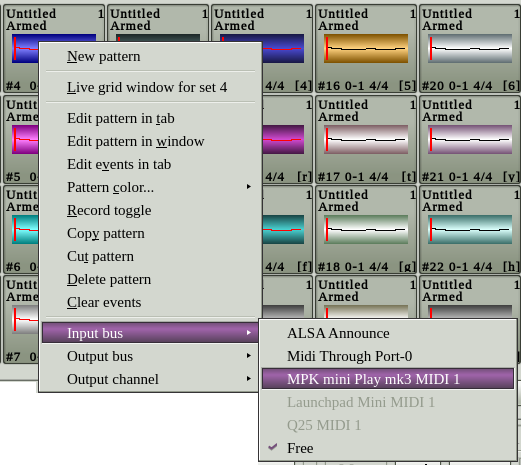
\includegraphics[scale=0.65]{main-window/slot-inputt-buss.png}
   \caption{Input Bus Popup Menu (as of 0.99.9)}
   \label{fig:slot_input_bus}
\end{figure}

   \itempar{Input Bus}{pattern!input buss}
   As of version 0.99.9, \textsl{Seq66} supports an
   \textsl{optional} input buss setting for each pattern.
   This setting is not available in the pattern editor due to lack
   of room, so this popup menu is the only way to get to this option.
   Normally, the "current" pattern, which is the one opened in
   the pattern editor, is the only one accepting input when
   recording is activated.

   By setting an input buss, incoming MIDI events can be routed to
   the pattern that is set to accept input from that buss.
   As the figure shows, the full set of input ports is shown.
   Some are disabled. (The "ALSA Announce" buss, should be disabled; this
   is a bug.)

   In the figure, the "Input B" pattern will accept events from
   the \textsl{KORG nanoKEY2} keyboard.
   If the \textbf{Free} entry is selected (the default), then
   the pattern will accept input from any MIDI input port.

   \textbf{Important}:
   \begin{itemize}
      \item If a MIDI input device is not enabled in the port list,
         it will not work as an input buss.
      \item If a MIDI input device is defined as an automation controller for
         \textsl{Seq66}, it will not work as an input buss.
      \item To disable the usage of input-buss routing, set the input buss
         to \textbf{Free} for all patterns, then save and reload the file.
      \item To record normally to a pattern, open the patter for recording
         and use a MIDI device that has \textsl{not} been assigned as
         a pattern's input buss.
   \end{itemize}
   
\subsubsection{Pattern}
\label{subsubsec:patterns_pattern_filled}

   A filled pattern slot is referred to as a \textsl{pattern}
   (or \textsl{track}, \textsl{loop}, or \textsl{sequence}).
   A pattern is shown in the pattern grid as a filled box with a number of
   items of information surrounding it.  Here are the items shown:

   \begin{itemize}
      \item \textbf{Pattern Name}. Top left.
         \index{pattern!name}
         This line, in the upper left of the pattern slot, contains the name or
         title of the pattern, for reference when juggling a number of
         patterns.
      \item \textbf{Pattern Status}. Second line.
         \index{pattern!status}
         Underneath the pattern-name is the status of the pattern, such as
         "Armed", "Muted", or "Queued".
         This status is useful when the Qt theme coloring makes the exact
         status difficult to determine.
      \item \textbf{Pattern Length}. Top right.
         \index{pattern!length}
         The length of the pattern, in measures, is shown in the upper
         right corner of the pattern slot.
         If the pattern has been modified, an \textbf{asterisk}
         appears after the
         number.
         Otherwise, if the loop-count for the pattern is greater than 0, 
         then an \textbf{plus sign} is shown.
         Remember that a pattern loop-count of 0 means the pattern can repeat
         "forever".
      \item \textbf{Notes or Fingerprint}. Center.
         \index{pattern!contents}
         The contents of the pattern, in the central box,
         provide a distinguishable representation of the notes or events in the
         pattern.
         The notes are shown in the center, inside a "progress box" that
         can also be colored, or not shown at all.
         Long patterns can be replaced by a much shorter "fingerprint", for
         faster drawing.
         Tempo events are indicated by a small circle.
         \index{empty pattern}
         An pattern with no playable events will not needlessly scroll.
         However, if a pattern has even a single event (say, a program change),
         it will scroll.
      \item \textbf{Progress Cursor}. Center.
         At the left of each center box is a vertical line, waiting for
         playback to start so that it can move through the pattern, again and
         again.
         When the song is playing, this vertical bar
         tracks the position of the playback of the pattern or loop; it
         returns to the beginning of the box every time the pattern starts
         over.
      \item \textbf{Sequence Number}. Bottom left.
         This number is shown at the bottom left of the pattern slot.
         Pattern numbers, by default, range from 0 to 31.
         Note how it varies fastest by row (top to bottom).
      \item \textbf{Bus-Channel}. Bottom, second from left.
         \index{pattern!bus-channel}
         This pair of numbers shows the the MIDI buss number, a dash, and
         the MIDI output channel number.
         For example, "0-2" means MIDI buss 0 (re 0), channel 2 (re 1).
         \index{pattern!free channel}
         If the channel is an "F", this means that the pattern has no specified
         output channel, and can play on all channels.
         This "free" channel concept is useful for applying Program Changes and
         Volume controls to many channels at once.
      \item \textbf{Beat/Beat Width}. Bottom, third from left.
         \index{pattern!beat}
         This pair of numbers is the standard time-signature of the pattern,
         such as "4/4" or "3/4".  The first number is the beats-per-measure,
         and the second is the size of the beat, here, a quarter note.
      \item \textbf{Shortcut Key}.  Also known as the
         \textbf{hot key}, this symbol is shown at the bottom right of the
         slot, in square brackets for better visibility.
         The key noted in the lower-right corner of the pattern is a "hot-key"
         that can be pressed to toggle the mute/unmute status of that pattern.
         This action is an alternative to
         \textsl{left-click} on the pattern.
         This hot-key can also be used to open the pattern in a pattern editor
         or in the event editor.
         Other actions are supported by changing the 
         \textbf{loop mode}.
%        (see \sectionref{paragraph:patterns_recording_modes}).
      \item \textbf{Armed}. Highlight color of button.
         Button highlighting indicates that the pattern is armed
         (unmuted), and will play if playback is initiated in the pattern
         \index{live mode}
         window in live mode.
         An item is armed/disarmed by a
         \textsl{left-click} on it, or by using the
         button's hot-key.
      \item \textbf{External Frame}. \textsl{Shift-left-click}.
         \index{shift left click}
         If the \texttt{Shift} key is held during a
         \textsl{left-click} on a pattern,
         the corresponding set's \textbf{Live} frame is brought up.
   \end{itemize}

   \index{pattern!left click}
   \textsl{Left-click} on an filled pattern box will toggle the status of the
   pattern between muted (white background) and unmuted (black background).
   If the song is playing via the main window, toggling this status makes
   the pattern stop playing or start playing.  The armed status
   can also be toggled using hot-keys and MIDI controls.

\subsubsection{Pattern Keys and Clicks}
\label{subsubsec:patterns_pattern_keys_and_clicks}

   This section recapitulates all the clicks and keys that perform actions
   in the Pattern windows.  Some additional clicks and keys are noted here
   as well.

\paragraph{Pattern Keys}
\label{paragraph:patterns_pattern_keys}

   \index{keys!hot}
   \index{keys!shortcut}
   Each pattern in the patterns panel can have a hot-key or shortcut-key
   associated with it.

   \index{keys!pattern toggle}
   \textbf{Pattern Toggle}.
   Like a \textsl{left-click}, for each pattern, its assigned hot-key will
   also toggle its status between muted/unmuted (armed/unarmed).
   Here is the normal layout of patterns, which was built into
   \textsl{Seq24}'s "DNA":

   \begin{verbatim}
      [  0 ] [  4 ] [  8 ] [ 12 ] [ 16 ] [ 20 ] [ 24 ] [ 28 ]
      [  1 ] [  5 ] [  9 ] [ 13 ] [ 17 ] [ 21 ] [ 25 ] [ 29 ]
      [  2 ] [  6 ] [ 10 ] [ 14 ] [ 18 ] [ 22 ] [ 26 ] [ 30 ]
      [  3 ] [  7 ] [ 11 ] [ 15 ] [ 19 ] [ 23 ] [ 27 ] [ 31 ]
   \end{verbatim}

   There is an alternate (and fairly new) mapping that can be enabled
   using the \texttt{swap-coordinates} option in the 'usr' file.
   See \sectionref{subsubsec:usr_file_user_interface_settings}.
   Below is the default keyboard "grid" that is
   mapped to the loops/patterns on the screen-set.

   \begin{verbatim}
      [ 1 ][ 2 ][ 3 ][ 4 ][ 5 ][ 6 ][ 7 ][ 8 ]
      [ q ][ w ][ e ][ r ][ t ][ y ][ u ][ i ]
      [ a ][ s ][ d ][ f ][ g ][ h ][ j ][ k ]
      [ z ][ x ][ c ][ v ][ b ][ n ][ m ][ , ]
   \end{verbatim}

   These characters are shown in the lower right corner of each
   pattern, as an aid to memory.
   This grid can be changed in the 'ctrl' file in the
   \texttt{[loop-control]} section.
   However, it is best to leave this setup as is, except for the key-swapping
   needed for alternative keyboard layouts like "QWERTZ".

   \index{keys!pattern shift}
   \textbf{Pattern Shift}.
   A "shift" functionality is available for the
   mute/unmute hot-keys when a set is larger than 32 patterns.
   \index{keys!slash}
   \index{variset!slash key}
   Normally, pressing the \texttt{1} key will toggle
   sequence 0.  If preceded by one slash key (\texttt{/}), then sequence 32
   will be toggled.  If preceded by two slash keys, then sequence 64 will be
   toggled.  This features supports using set sizes of 32, 64, and 96 patterns.

   \index{keys![}
   \index{keys!decrement set}
   \index{keys!screenset down}
   \textbf{Screenset Increment and Decrement}.
   The "\texttt{[}" and
   \index{keys!]}
   \index{keys!increment set}
   \index{keys!screenset up}
   "\texttt{]}" keys on the keyboard decrement or increment the set number.

   \index{keys!alt}
   \index{keys!snapshot}
   \textbf{Snapshot}.
   When a snapshot key is pressed, the state of the patterns
   (armed versus unarmed) is saved.  While the
   snapshot is in force, one can then change the state of the patterns
   (using the keyboard or MIDI controls, \textsl{not} the mouse)
   to change how the song plays.  When the snapshot mode is exited, the
   original saved state of the patterns is restored.

   Unlike in \textsl{Seq24}, the \texttt{Alt} keys are not used.
   In addition, the snapshot key acts like a toggle... no need to hold it down.
   Lastly, there is only one snapshot key slot.
   Our preference is to use something that does not trigger desktop
   commands, perhaps "\texttt{F11}" or "\texttt{F12}", or one of the keys in
   the keypad.
   Configured in the 'ctrl' file
   \texttt{[automation-control]} section.

   \index{keys!right ctrl}
   \index{keys!queue}
   \index{queue!temporary}
   Pressing the "queue" key and then hitting a pattern hot-key
   will queue an on/off toggle for a pattern when the end of the loop is
   reached.
   This is the "queue" functionality.
   This means that the change in state of the pattern will not take hold
   immediately, but will kick in when the pattern restarts.
   This pending state is indicated by coloring the central box of the
   pattern grey.
   Please note the "keep queue" functionality and
   the "one-shot queue" functionality described below.

   A light-grey color is used to show a "one-shot" queue.
   The one-shot queue can only turn a pattern on, and it
   will force the pattern off after one play.
   Queue also works for mute/unmute pattern sets ("groups"); in this case,
   every sequence will toggle its status after its individual loop ends. 
   \index{keys!avoid ctrl/alt}
   We do \textbf{not}
   recommend using \texttt{Ctrl} or \texttt{Alt}
   keys for pattern control.  They conflict with application or desktop
   settings.

   \index{keys!keep queue}
   \index{queue!keep}
   Pressing the "keep queue" hot-key
   \index{rc file}
   assigned in the 'rc' file activates a "sticky" queue mode.
   In this mode, pressing a pattern key immediately turns on queuing, instead
   of mute/unmute.  And multiple patterns can be handled in this way at the
   same time.
   Keep-queue persists until one clicks the queue hot-key again,
   or changes the active (viewed) screen-set. 
   \index{queue!cancel}
   “Keep queue” mode is cancelled by pressing the normal queue hot-key.
   There is also a \textbf{Q} button for the same purpose.
   Also note the "queued replace/solo" functionality, described a bit later.

   \index{one-shot queue}
   \index{keys!one-shot queue}
   \index{queue!one-shot}
   Thanks to \textsl{Kepler34}, we have "one-shot queue"
   functionality.  This one-shot setup queues a pattern up for unmuting only,
   and, once the pattern has played, it is automatically muted.  This process
   is easier than having to unqueue the pattern manually before the next
   playback.
   This hot-key can be changed in the 'ctrl' file.

   \index{keys!replace}
   The "replace" hot-key sets a form of muting/unmuting.
   When the "replace" hot-key is
   pressed, then pressing a pattern's hot-key,
   that sequence is unmuted, and all of the other sequences are muted.
   "Replace" is a form of "solo".
   "Replace" is also implemented via MIDI control,
   where the MIDI control can be activated, but then the user has to select
   the desired sequence.  

   \index{queue!replace}
   \index{queue!solo}
   \textsl{Seq66} provides an extension to the replace/solo functionality
   that is called "queued-replace" or "queued-solo".  In this feature, when
   the "keep queue" function is activated, the replace function is queued so
   that it does not occur until the next time the patterns loop.
   And queued-replace provides a form of snapshot, limited to the
   \textsl{current} screen-set.
   Here are the steps:

   \begin{enumber}
      \item Start playback with some patterns on. 
      \item Press and release
         the "keep queue" hot-key.  This puts the application into "queue" mode.
         It is indicated via a "\textbf{Q}" button.
      \item Press and hold the "replace" hot-key.
      \item Click the desired pattern hot-key.  Observe that it arms or
         stays on, and that the other playing patterns show the "queued" color
         (grey).  At the end of the loop, they turn off, and the "replace"
         pattern is now solo.
      \item Click the same pattern hot-key again.  Observe that the other
         patterns that were toggled off are now queued to be toggled on at the
         next loop.  Steps 4 and 5 can be repeated endlessly.
      \item To end
         \index{queue!clear}
         \index{queue!end}
         the "queued-replace" mode, click the normal "queue"
         hot-key.  Also, changing the active screen-set ends "queue-replace"
         mode.  It does \textsl{not} end normal queue mode, to preserve the
         behavior found in \textsl{Seq24}.
         One needs to clear the queue mode in order to select another pattern
         to solo.
   \end{enumber}

   Before pressing the "keep queue" key, patterns 33 ("\textbf{q}")
   and 34 ("\textbf{a}") are
   unmuted, while the desired replace pattern, 32 ("\textbf{1}") is off.
   Then the user presses (and holds) the "replace" key, then clicks the
   "\textbf{1}" key.
   This puts all unmuted patterns, plus the muted
   replace pattern as well, into queue mode, as shown by the grey panels.
   When the progress bar reaches the end of the pattern, pattern 32 will go on,
   and patterns 33 and 34 will go off.
   If the replace-pattern is already on, it is not queued, as
   there's no need to turn it on.

   If, while in queue mode, the replace key is held and
   "\textbf{1}" is pressed again,
   the other patterns will be queued, and will turn on again.  Thus, the
   solo status of the replace pattern can be toggled at will, until queue mode
   is exited by pressing and releasing the normal "queue" key.
   If the replace key is \textsl{not} held down, and another pattern's replace
   hot-key is pressed, that pattern will be queued normally.
   If one wants to change the solo functionality to a different pattern,
   simple hold the replace key and click on a different pattern.  The new
   arrangement of soloing is memorized.
   One can clear the queue mode by pressing the normal queue key.

   There are more keys defined in the 'ctrl' file, and it is
   worth figuring out what they do, if not documented here.
   Also see the installed \texttt{control\_keys.ods} spreadsheet.
   For a couple of short, but good, video tutorials about using arming,
   queuing, and snapshots, see reference \cite{wootangent1}.

\paragraph{Other Pattern Clicks}
\label{paragraph:patterns_pattern_clicks}

   \index{pattern!left click}
   \index{pattern!mute toggle}
   \textsl{Left-click} on a pattern-filled box will change its state
   \index{pattern!mute}
   \index{pattern!unmute}
   from muted (white background) to playing (black background), whether
   the sequencer is playing or not.

   \index{pattern!left click-drag}
   \textsl{Left-click-hold-drag} on a pattern, drags it to a different
   pattern on the grid.
   The box disappears while dragged, and reappears in the new location when
   dropped.  However, a pattern \textsl{cannot} be dragged if its
   \textbf{Pattern Editor} window is open.

   \index{pattern!right click}
   \textsl{Right-click} on a pattern brings up the appropriate context menus, as
   discussed earlier, depending on whether the pattern box is empty or
   filled.

   \index{pattern!middle click}
   \textsl{Middle-click} on a pattern will bring up the pattern
   in the \textbf{Editor}
   tab in the main window.

   \index{pattern!shift-left-click}
   \index{shift-left-click live-frame}
   \textsl{Shift-left-click} on a pattern will open up an external
   live-frame for the
   set having the same number as the pattern.

   \index{pattern!ctrl-left-click}
   \index{ctrl-left-click new pattern}
   \textsl{Ctrl-left-click} on a pattern will create a new pattern, just like
   double-click will (if enabled).

   \index{solo!true}
   \index{pattern!alt-left-click}
   \index{patterns panel!inverse muting}
   \index{patterns panel!solo}
   \index{alt-left-click solo}
   There is a truer "Solo" functionality in the Patterns
   Panel and the Song Editor.  To "solo" a pattern, move the mouse cursor
   over the pattern, hold the \texttt{Alt} key, and left-click the pattern.
   This will turn off all the other patterns, so that the selected pattern ins
   the only one playing.
   We still need to work on reversing it exactly, but
   mute-groups can be used for that purpose.
%  Holding the \texttt{Alt} key and clicking the same
%  pattern again will unmute all of the other patterns.

\paragraph{Metronome}
\label{paragraph:patterns_metronome}

   \index{metronome}
   Also shown in the figure is a \textbf{Metronome} button.
   This is a feature new with \textsl{Seq66} version 0.99.0, and still has a few
   minor issues to work out, but it works.
   The metronome has a number of configurable items.
   See \sectionref{subsubsec:configuration_rc_metronome}.

   Clicking the metronome button turns the metronome on and off.
   To use the metronome (once configured), click the button to enable it,
   then start playback.
   It can be turned on and off during playback.
   It is always available, stored as a hidden automatically-generated
   pattern.

\paragraph{Background Recording}
\label{paragraph:patterns_background_recording}

   \index{background recording}
   Also shown in the figure is a \textbf{Background Recording} button.
   This feature still has a few
   minor issues to work out, but it works.

   The recorder has a number of configurable items.
   See \sectionref{subsubsec:configuration_rc_background_recording}.
   Background recording needs to be enabled in the configuration.
   Otherwise, the background-recording button is disabled.

   When enabled, press the background-recording button.  Now all events on the
   given input buss will be recorded, even if playback is not started.
   Better to start playback after enabling recording!

   Once one is satisfied with the recording, stop playback, then
   click the background-recording button again.
   If any events have been recorded, then they are pasted into a new pattern in
   the next available pattern slot.
   There, they can be edited or deleted.
   Note that the background pattern is muted while recording.
   We will change how it works based on user feedback.

\paragraph{Pattern Loop Modes}
\label{paragraph:patterns_loop_modes}

   \textsl{Seq66} has always had the feature of turning on recording, including
   quantized recording, in the pattern editor.
   Now, it also provides for
   \index{loop!modes}
   loop modes.  With this new feature, the normal loop muting/unmuting
   functionality of the \textbf{Live Grid} can be changed to allow the toggling
   of recording or other actions to be applied to each pattern.
   This new functionality is enabled by two buttons in the main window grid and
   by two refactored keystroke/MIDI controls ("Record" and "Quan Record").
   The normal mode (mute/unmute) is called \textbf{Loop}.

   \begin{itemize}
      \item \textbf{Loop}.
         This mode is the legacy and long-time standard mode of
         \textsl{Seq24}, \textsl{Sequencer64}, and \textsl{Seq66}.
         When in this mode, a click on a pattern slot, a loop-control
         keystroke, or a loop-control MIDI event, will change the mute/unmute,
         armed/unarmed status of a pattern.
      \item \textbf{Record}.
         A click/key on the pattern turns on recording for that pattern.
      \item \textbf{Copy}.
         Copies the selected pattern into the clipboard.
      \item \textbf{Paste}.
         Pastes the clipboard into the selected pattern.
      \item \textbf{Clear}.
         Removes the events from the selected pattern.  Careful!
         Not yet ready.
      \item \textbf{Delete}.
         Deletes the selected pattern.  Careful!
      \item \textbf{Thru}.
         Turns on the MIDI Thru functionality of the selected pattern.
      \item \textbf{Solo}.
         Soloes the selected pattern.
      \item \textbf{Cut}.
         Deletes the selected pattern and copies it into the clipboard.
      \item \textbf{Double}.
         Doubles the length of the selected pattern.
         Not yet ready.
   \end{itemize}
   It has been supplemented by four recording modes.
   Here are the modes:

   \begin{itemize}
      \item \textbf{Overdub}.
         \index{merge}
         \index{overdub}
         \index{record!merge}
         \index{record!overdub}
         This mode is selected by clicking on the \textbf{Loop} button,
         then using the \textbf{Record} control.
         These commands cycle between all the modes in this list.
         Overdub is the same as the \textbf{Merge} option in the 
         pattern editor.
         Clicking a grid will turn on/off the overdub recording mode
         for that pattern.
         It enables recording that accumulates note events in each pass of
         looping through the pattern.
      \item \textbf{Overwrite.}
         \index{overwrite}
         \index{recording!overwrite}
         This mode causes the grid button to turn on overwrite recording.
         When the loop restarts over and a note is pressed,
         then the existing notes in that loop are erased,
         and the new note is added.
      \item \textbf{Expand}.
         \index{expand}
         \index{recording!expand}
         This mode causes the grid button to turn on expand recording.
         Once the end of the loop is near, whether or
         not any notes are being input, another measure is added to the length
         of the loop.
      \item \textbf{One-shot}.
         \index{one-shot}
         \index{recording!one-shot}
         When this option is set, with the record button on, and no pattern
         playing, recording won't start until a note comes in, and when the
         first note comes in, the progress bar starts at the left (time 0).
         As each new set of notes at the same timestamp come in, the
         notes are recorded and the current time advances by one snap value.
         Once the end of the pattern lenght is reached, recording is turned
         off.
      \item \textbf{One-shot Reset}.
         \index{one-shot reset}
         \index{recording!one-shot reset}
         When the \textbf{One-shot} option is selected, this new option
         is enabled.
         When clicked, three things happen:
         \begin{itemize}
            \item All the (note) events just recorded are \textsl{erased}.
            \item One-short counters/flags are \textsl{reset}.
            \item Recording is turned \textsl{back on}.
               Thus, one can easily re-do a one-shot recording.
         \end{itemize}
   \end{itemize}

   Once the recording mode is turned on, then the recording type comes into
   play:

   \begin{itemize}
      \item \textbf{No Quan}.
         Incoming events are recorded as is.
         Plain recording, events recorded with timestamps unaltered.
         Indicated by a red circle.
      \item \textbf{Quantize}.
         When recording, quantize the incoming events.
         Incoming events are quantized to the snap value of the pattern.
         Indicated by a red circle and a "Q" inside it in a pattern slot.
      \item \textbf{Tighten}.
         A weaker version of \textbf{Quantize}.
         Incoming events are partially quantized to the snap value of the
         pattern.
         Indicated by a red circle and a "T" inside it in a pattern slot.
         This mode is accessible only via this recording mode; there
         is no such button in the pattern editor.
   \end{itemize}

\subsection{Patterns / Bottom Panel}
\label{subsec:patterns_panel_bottom}

   The first line of the bottom panel contains the \textbf{Set Name}
   of the current set, which is editable.
   It contains a button with an exclamation point (\textbf{!}), which
   can be used to reset the play-set (the total of all patterns that are loaded
   for playback) to the patterns in the current set.
   The \textbf{Set} spin-box can be used to change the current set.

   \begin{enumber}
      \item \textbf{Set Name}
      \item \textbf{Set Reset}
      \item \textbf{Set}
   \end{enumber}

   \setcounter{ItemCounter}{0}      % Reset the ItemCounter for this list.

   \itempar{Set Name}{pattern!set name}
   Each of the 32 available screen-sets can be given a name by entering it
   into this field.  This name is saved with the MIDI file.

   \itempar{Set}{pattern!set number}
   This spin widget selects the current screen-set.  The values in this
   field range from 0 to 31 (less if the set-size is a larger value),
   and default to 0.

   \itempar{Set Reset}{pattern!set reset}
   \textsl{Seq66} has a new feature whereby multiple sets can play at once.
   This button, an exclamation point, will reset the playback to the patterns
   in the current set.

   The bottom panel of the Patterns window provides way to control the
   overall playback of the song.  It has changed quite a bit over the last few
   versions of \textsl{Seq66}, and we have not yet caught up with the
   diagrams. And the Qt user-interface adds more changes.
   Refer to the diagram of the whole window, for now.
   It has a number of items:

   \begin{enumber}
      \item \textbf{Panic!}
      \item \textbf{Stop}
      \item \textbf{Play and Pause}
      \item \textbf{Loop}
      \item \textbf{Song Record}
%     \item \textbf{Song Record Snap}
%     \item \textbf{Log Tempo}
%     \item \textbf{Record Tempo}
      \item \textbf{Keep-Queue Status}
      \item \textbf{Toggle Song/Live Mode}
      \item \textbf{Tap Tempo}
      \item \textbf{BPM}
   \end{enumber}

   \setcounter{ItemCounter}{0}      % Reset the ItemCounter for this list.

   \itempar{Panic!}{pattern!panic}
   This new button stops the song and sends MIDI Off messages on all notes.

   \itempar{Stop}{pattern!stop}
   The red square button stops the playback of the song and all its patterns.
   \index{keys!esc (stop)}
   The keystroke for stopping playback is the \texttt{Escape} character; it
   stops playback and rewinds to the beginning of the song.
   The \texttt{Space} keystroke will do the same thing if playback is in
   progress; it is effectively a playback toggle key.

   \itempar{Play and Pause}{pattern!Play}
   \index{pattern!Pause}
   The green triangular button starts the playback of the whole song.
   \index{keys!space (play)}
   The keystroke for starting playback is the \texttt{Space} character by
   default.  It also stops playback, also rewinding the song to the beginning.
   \index{pause}
   The Pause button toggles playback without rewinding the song.
   A Pause key (by default, the period) is also defined.

   \itempar{Loop}{pattern!loop}
   If this button is active, then the playback will loop
   between the "L" and "R" markers in the pattern editor or the song editor
   time-lines.
   As with the "L" and "R" markers in the pattern editor, this can
   be placed via left and right mouse clicks.
   Note that the "L" and "R" markers can be selected via the keyboard using
   their respective shifted key.  Once selected, the marker can be moved left
   or right using the left and right arrow keys.

   \itempar{Song Record}{pattern!song record}
   Song-recording in \textsl{Seq66} is adopted from the
   \textsl{Kepler34} project.
   This feature takes live muting changes and records them as
   triggers in the \textbf{Song Editor}.
   The default hot-key for this function is \texttt{P}.
   This feature does not honor queuing...
   rather than waiting until the end of the pattern when the queuing takes
   effect, the trigger recording starts immediately.

%  \itempar{Song Record Snap}{pattern!song record snap}
%  This button toggles snapping the beginning and end of a recorded trigger to
%  the nearest beat.  There is no hot-key for this button at this time.
%  And, in fact, at present, song-record snap is alway in force.

   \itempar{BPM}{pattern!BPM}
   The spin widget adjusts the "beats per minute" (BPM) value.  The
   range of this field is from 1 bpm to 600 bpm, with a default value of
   120 bpm.
   Although this field looks editable, it is not.  Most keystrokes
   that are entered actually toggle one of the pattern boxes.
   However, the following keys can also modify the BPM in small increments:
   \index{keys!semicolon}
   The \texttt{semicolon} reduces the BPM;
   \index{keys!apostrophe}
   The \texttt{apostrophe} increases the BPM.
   Also, if one \textsl{right-clicks} on the
   \textbf{Up} button, the BPM advances to its largest
   supported value, and if one \textsl{right-clicks} on the
   \textbf{Down} button, the BPM
   advances to its lowest value.
   MIDI control for this value is also available.
   The precision of the BPM value can be set to 0, 1, or 2
   decimal places, and the increment values for the step size (small)
   or page size (large) of the BPM spinner can be configured in the 'usr' file.

   \itempar{Tap Tempo}{pattern!tap tempo}
   This control is clicked in time with a tune, to set the
   tempo based on the tempo of the clicks.  Once clicked, the label of this
   button increments with every click, and the \textbf{BPM} field updates to
   display the calculated tempo.  If the user stops tapping for 5 seconds, the
   label reverts to 0, the BPM value keeps its final value, and the user can
   try tapping the tempo again, or accept the current value.
   Tapping can also be done using the keystroke defined
   in the 'ctrl' file.
   It defaults to the "\texttt{F9}" key.

   \itempar{Keep-Queue Status}{pattern!keep-queue}
   This item is the \textbf{Q} button.
   It provides a visual way to know the current state of keep-queue, and is
   activated either by clicking on it or by pressing the assigned keep-queue
   key.

   \itempar{Toggle Song/Live Mode}{pattern!song/live}
   Pressing this button toggles between the song mode and live mode.
   Note that the default mode is configurable, and \textsl{Seq66} can go into
   song mode when a loaded MIDI file has triggers, if configured to do so.

\subsection{Patterns / Multiple Panels}
\label{subsec:patterns_panel_multiple}

   Multiple patterns-panels can be created in addition to the one in the "Live"
   tab.  The live set-up and set-down keystrokes, as well as their MIDI control
   counterparts (both defined in a 'ctrl' file).
   apply only to the main window.

\subsection{Patterns / Variable Set Size}
\label{subsec:patterns_panel_variset}

   \index{variset}
   This option, informally known as "variset", allow some changes in
   the set size and layout from the default 4x8 = 32 sets layout.
   The row count can be set from 4 to 8, and the column count can be set to 8
   to 12.  Note that the set size can only be \textsl{increased} by these
   settings.

   \textbf{Warning:}
   \textsl{seq24} was fairly hardwired for supporting 32 patterns per
   set, and there are still places where that is true.  Thus,
   consider this option to be experimental.

   The \texttt{-o sets=8x8} option can be used to set this mode.
   These settings can be made permanent in the 'usr' file.
   In that file, the options modified are \texttt{mainwnd\_rows} and
   \texttt{mainwnd\_cols}.

   Generally, it is recommend to stick with the 4x8 (32 patterns/set),
   8x8 (64 patterns/set), and 8x12 (96 patterns/set).  This works best with the
   existing set of 32 hot-keys.

   Also note that the Qt 5 user-interface also supports "variset", whether in
   the main window or in the external live-frame.  In addition, the Qt windows
   can be resized and still show reasonable renditions of the pattern-slots.

\subsection{Patterns / Set Handling}
\label{subsec:patterns_panel_set_handling}

   Let's go through an example using the \texttt{Home} key (or whatever key is
   configured as the \textbf{Set Playing Screenset} key.)

   \begin{enumber}
      \item Load a song with more than one screen-set.
      \item Unmute the pattern(s) in the first set and start playback.
      \item Use the "\texttt{]}" (\textbf{Screenset Up}) key to move to the next
         set.  Note that the first set is still playing.  Also note that the
         now-current set is \textsl{not} playing.
      \item Press the \texttt{Home} key.
         Note that the first set turns off, and the current set turns on.
         These steps can be repeated at will.
      \item Finally, hit the \texttt{F8} (\textbf{Toggle Mutes}) key.
         Note that all tracks on all sets toggle muting each time this key is
         pressed.
   \end{enumber}

%-------------------------------------------------------------------------------
% vim: ts=3 sw=3 et ft=tex
%-------------------------------------------------------------------------------


% Pattern Editor

%-------------------------------------------------------------------------------
% pattern_editor
%-------------------------------------------------------------------------------
%
% \file        pattern_editor.tex
% \library     Documents
% \author      Chris Ahlstrom
% \date        2015-08-31
% \update      2024-12-01
% \version     $Revision$
% \license     $XPC_GPL_LICENSE$
%
%-------------------------------------------------------------------------------

\section{Pattern Editor}
\label{sec:pattern_editor}

   The \textsl{Seq66} \textbf{Pattern Editor} can edit and preview a
   pattern, configure its buss, channel, transpose, musical
   scale, and many other settings.
   A slightly modified  version of the \textbf{Pattern Editor} appears in the
   \textbf{Edit} tab in the main window; the main window has to be expanded
   vertically to see all of the controls.
   The complete version can be brought up in an external window.

\begin{figure}[H]
   \centering 
   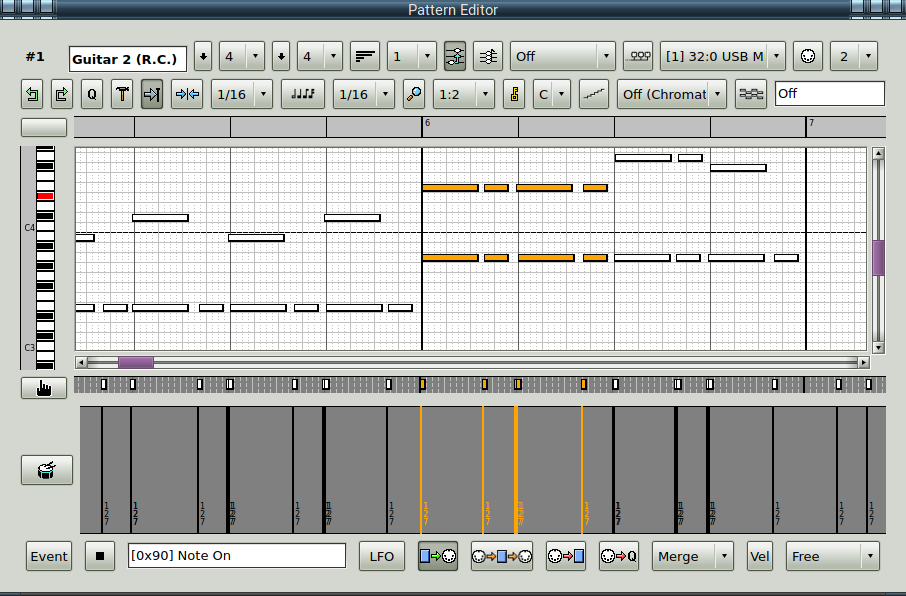
\includegraphics[scale=1.00]{pattern-editor/pattern-edit-window.png}
   \caption{External Pattern Editor Window}
   \label{fig:pattern_editor_window}
\end{figure}

   This figure does not show a recent new feature: for selected event,
   the orange data line is topped with a circular "grab handle" that can
   be used to change the amplitude of the data (e.g. velocity) being
   shown.
  
   The \textbf{Pattern Editor} is complex, and we will discuss the external
   window only since its features are a superset of the \textbf{Edit} tab.
   For exposition, we break the window into the following sections:

   \begin{enumber}
      \item \textbf{First Row}
      \item \textbf{Second Row}
      \item \textbf{Time}
      \item \textbf{Piano Roll}
      \item \textbf{Events Pane}
      \item \textbf{Left Buttons}
      \item \textbf{Data Pane}
      \item \textbf{Bottom Row}
      \item \textbf{Common Actions}
   \end{enumber}

   Before we describe this window, there are some things to recognize.
   First, if the pattern is empty when play is started, the progress bar will
   still move, so that the user can play a MIDI instrument and record new notes.
   Second, to add a note with the mouse, one must press the \textsl{right}
   mouse button (the pointer changes to a pencil) and,
   \textsl{while holding it}, press the left mouse button.
   Or click in the pattern editor, press the
   \index{keys!i}
   \index{keys!p}
   \texttt{p} key to select the "pencil" or "paint" mode,
   or
   \texttt{i} key to select "insert" mode (a la vi),
   then
   \index{mouse!left-click}
   left-click to add a note or
   \index{mouse!left-click-drag}
   left-click-drag to add multiple notes as the mouse moves.
   \index{keys!x}
   \index{keys!Esc}
   Press or release the right mouse button, or press
   \texttt{x} to "eXit" or "eXscape" from paint mode.
   \texttt{Esc} also exits paint mode if the pattern is not playing.
   If not in paint mode, then the window is closed, just like a dialog box.
   Another option is to press the "finger" button to toggle between note-entry
   and note-selection.
   Third, notes are drawn only with the length selected by the "notes" button
   near the top of the pattern window.  There are tricks to
   modifying the new notes that are described later.

   \textsl{Seq66} automatically scrolls
   horizontally through the sequence/pattern editor window when
   playback moves the progress bar outside of the current frame of data.  This
   feature makes it easier to follow patterns that are longer than a measure or
   two.
   One might want to print out the following figure to follow along.  There is
   a lot of functionality in this window.

\begin{figure}[H]
   \centering 
   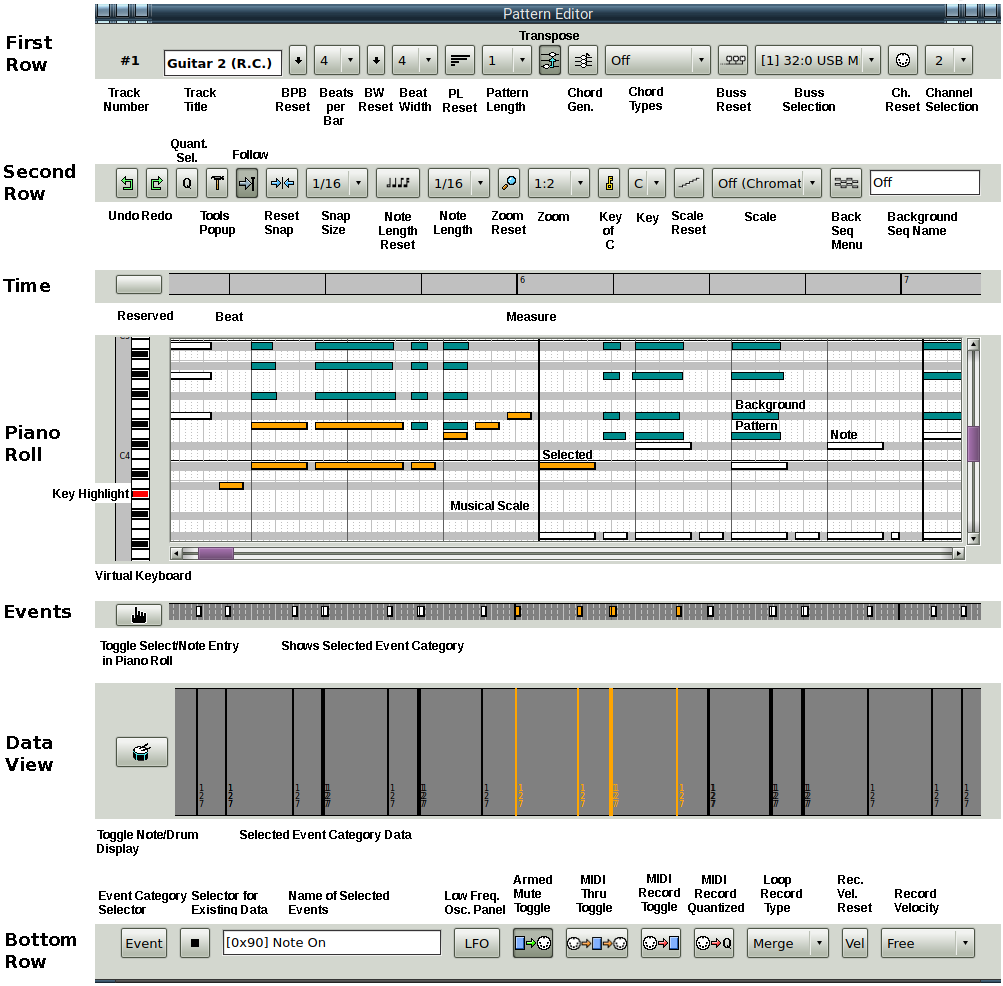
\includegraphics[scale=0.90]{pattern-editor/pattern-edit-window-annotated.png}
   \caption{Pattern Editor Window, Annotated}
   \label{fig:pattern_editor_window_annotated}
\end{figure}

   The arrow keys can be used to move left, right, up, or down.

   \index{keys!vi}
   \index{keys!hjkl}
   For \textsl{vi} users, the "h" (left), "j" (down), "k" (up), and "l" (right)
   keys can be used while any pane is in focus, and they act like the arrow
   keys.

\subsection{Pattern Editor / First Row}
\label{subsec:pattern_editor_first_row}

   The top bar (horizontal panel) of the Pattern (sequence) Editor
   lets one change the name of
   the pattern/loop/sequence/track, the time signature of the piece, how long
   the track is, and some other configuration items.

   \begin{enumber}
      \item \textbf{Track Number}
      \item \textbf{Track Name}
      \item \textbf{Add Time Signature Event} (see composite picture below)
      \item \textbf{Beats Per Bar Reset} and \textbf{Beats Per Bar}
      \item \textbf{Beat Width Reset} and \textbf{Beat Width}
      \item \textbf{Pattern Length Reset} and \textbf{Pattern Length}
      \item \textbf{Chord Types}
      \item \textbf{Buss Reset} and \textbf{Buss Selection}
      \item \textbf{Channel Reset} and \textbf{Channel Selection}
   \end{enumber}

   \setcounter{ItemCounter}{0}      % Reset the ItemCounter for this list.

   \itempar{Track Number}{pattern editor!number}
   This item shows the sequence/track/pattern/loop
   number, to make it easier to pick it out when a lot of patterns are being
   edited at once.

   \itempar{Track Name}{pattern editor!name}
   Provides the name of the pattern.
   This name should be short and memorable.
   It is displayed in the \textbf{Live Grid} (the \textbf{Patterns Panel}),
   on the top line of its pattern slot.

   \itempar{Add Time Signature Event}{pattern editor!time signature}
   This button is shown in the composite picture in
   \sectionref{subsec:pattern_editor_time}, to the left of the beat
   selector.
   When either the beats/bar or beat width values (see below) are changed,
   and the progress marker is at time 0, then the change is
   saved as a Time Signature Meta event at time 0. Additional changes there
   overwrite that event.
   There are interactions between the beats/bar, beat-width, and the length (in
   measures) of the pattern.
   Generally, if both the beats/bar and beat-width are to be changed,
   it is better to change the beat-width first.
   In any case, the measures might have to be adjusted as well.
   It is better to get all the time signatures in place before adding notes.
   To add time signatures at later times in the tune, this must be done:

   \begin{enumber}
      \item Move the mouse cursor to the \textsl{top half} of the time pane;
         the cursor will change to a vertical arrow. Click at the desired time
         and observe the red progress line.
      \item Change the beats-per-measure, if desired.
      \item Change the beats-width, if desired.
      \item Clock the \textbf{Add Time Signature} button to log the
         new time signature.
   \end{enumber}

   It adds a time-signature Meta event and adjusts the pattern
   length (if needed) at once.
   The new time signature should appear in the data and event panes as well.

   \itempar{Beats Per Bar}{pattern editor!beats/bar}
   \index{beats per bar}
   Specifies the number of beat units per bar in the time signature.
   The possible values range from 1 to 16, if the drop-down menu is used.
   Arbitrary values up to 32 can be entered by typing the number.
   The "Reset" button resets the value to 4.

   \itempar{Beat Width}{pattern editor!beat width}
   \index{beat width}
   Specifies the size of the bottom beat unit of the time signature:
   1 for whole notes; 2 for half notes; 4 for quarter notes; 8 for eight notes;
   16 for sixteenth notes; and 32 for thirty-second notes.
   The whole time signature is display at the bottom center of the
   corresponding pattern slot in the \textbf{Live Grid}.
   Arbitrary values up to 32 can be entered by typing the number.
   The "Reset" button resets the value to 4.

   Now, although the combo-box provides only beat-widths that are the
   MIDI-standard power of 2, the number can be edited for any number.
   A warning prompt appears, and if OK'ed, then the non-standard beat-width is
   set, but it is not added as a time-signature event.
   Instead, it is stored as a SeqSpec event for \textsl{Seq66}.

   \itempar{Pattern Length}{pattern editor!length}
   Sets the length of the current pattern, in measures.
   The possible values range from 1 to 64.
   Arbitrary values up to 1024 can be entered by typing the number.
   \textsl{However}, when opening or importing a non-\textsl{Seq66}
   MIDI tune, the length of each track will be used, and so other values
   are possible.

   Bringing up a pattern less than one measure or bar in
   length in the pattern editor will adjust the pattern to pad it to the
   length of one measure.
   \index{pattern editor!progress bar}
   \textsl{Seq66} will, when it reads such a short pattern
   from a MIDI file,

   \index{expand}
   \index{recording!expand}
   A feature from user \textsl{stazed} allows the pattern to expand
   indefinitely while the user inputs MIDI from a controller, via the
   \textbf{Expand} option of the \textbf{Loop Record Type}.
   This works in \textbf{Live} mode or \textbf{Song} mode.
   \textsl{Note: the following is no longer true.
   Instead, the pattern extends continually; these provides a more
   reasonable user experinece:
   The pattern is not extended until events come in.
   Thus, the pattern is only as long as the last measure when a note comes in.}
   Once playback starts, the progress bar moves forward.
   Notes are recorded they are enter.
   Once the end of the measure is neared, another
   measure is added, whether or not more notes are struck.
   The measure-count at the top of the editor shows the current number
   of measure.
   Once playback (and recording) stops, the user can either accept the
   final length, or change the length to a lesser number.
   If the lesser length will drop notes, a prompt will appear
   for the user to accept or reject the length change.

   \itempar{Chord Types}{pattern editor!chord types}
   \index{chord generation}
   This setting allows one to select a chord type (e.g. "major" or "minor").
   When active, a note is treated like the base note of the selected chord
   type, and extra notes are generated to create that chord.
   The \textbf{Chord Generation Reset} button is at the left of the
   \textbf{Data Pane}.

   \itempar{MIDI Out Device (Buss)}{pattern editor!midi out device}
   This setting specifies a virtual MIDI output buss or a
   MIDI output device set up by the computer and
   attached MIDI equipment.
   The button resets it to buss 0.
   Note that, if the pattern's selected buss is not found, this entry will be
   blank.  The user must select a valid buss from this dropdown.

   \itempar{MIDI Out Channel}{pattern editor!midi out channel}
   The \textbf{Channel Selection} setting selects the MIDI output channel.
   The possible values range from 1 to 16, plus \textsl{Free}, which means
   that the channels of the events are preserved, and are used as the output
   channel, a bit like an SMF 0 track.
   The editing channel is always channel 1.
   If instruments are assigned in the 'usr' configuration file
   to that device and channel, their names will be shown in the dropdown.

   In addition, this setting determines the channel applied when painting notes
   in the piano roll.  If set to "1" or "Free" (no channel), then channel 1 is
   applied.  Otherwise, if set to "2" through "16", that channel is applied.

\subsection{Pattern Editor / Second Row}
\label{subsec:pattern_editor_second_row}

   The second horizontal panel of the Pattern Editor provides a number
   of additional settings and functions:

   \begin{enumber}
      \item \textbf{Undo}
      \item \textbf{Redo}
      \item \textbf{Quantize Selection}
      \item \textbf{Tools Popup}
      \item \textbf{Follow Progress}
      \item \textbf{Reset Snap} and \textbf{Grid Snap}
      \item \textbf{Note Length Reset} and \textbf{Note Length}
      \item \textbf{Zoom Reset} and \textbf{Zoom}
      \item \textbf{Key Reset} and \textbf{Key of Sequence}
      \item \textbf{Scale Reset} and \textbf{Musical Scale}
      \item \textbf{Background Sequence}
   \end{enumber}

   \setcounter{ItemCounter}{0}      % Reset the ItemCounter for this list.

   \itempar{Undo}{pattern editor!undo}
   The \textbf{Undo} button rolls back any changes to the pattern from this
   session.  It will roll back one change each time pressed.
   \index{keys!ctrl-z}
   Pressing \texttt{Ctrl-Z} is the same as using the \textbf{Undo} button.

   \itempar{Redo}{pattern editor!redo}
   The \textbf{Redo} button will restore any undone changes to the pattern from
   this session.
   It will restore one change each time it is pressed.
   There is currently no redo key.

   \itempar{Quantize Selection}{pattern editor!quantize}
   This button quantizes the selected events as per
   the \textbf{Grid Snap} setting.

   \itempar{Tools}{pattern editor!tools}
   This button brings up a nested menu of tools for modifying selected
   events and notes.

   \begin{enumber}
      \item \textbf{Select Notes...}.
      Selects Note Ons, Note Offs, and Aftertouch.
      In order for notes to be modified by quantization or randomization,
      they need to be selected first, otherwise some menu entries are
      disabled..
      Notes can be selected in the piano roll of via this menu.
      This menu provides two note-selection options:
         \begin{itemize}
            \item \textbf{Select all}, selects all notes in the pattern;
               The \index{keys!ctrl-a} \texttt{Ctrl-A} will also select
               all of the events in the pattern editor.
            \item \textbf{Invert selection}, which inverts the selection of
               notes.
         \end{itemize}
      \item \textbf{Note timing/velocity...}. This menu
            offers three ways to tweak the timing of the selected notes:
         \begin{itemize}
            \item \textbf{Quantize}
               \index{quantize}
               quantizes the selected notes in time, the same way as the
               \textbf{Quantize} ("\textbf{Q}") button.
            \item \textbf{Tighten}
               \index{tighten}
               This operation merely a less strict form of quantization.
            \item \textbf{Jitter}
               \index{jitter}
               Jittering modifies the timing of a note by adding or subtracting
               a small random of time.
            \item \textbf{Randomize velocity}
               \index{randomize}
               This operation modifies the velocity of a note by a small
               amount.
         \end{itemize}
      \item \textbf{Pitch transpose} allows uniform transpostion
         regardless of the key and scale in force for the pattern.
         \index{modify pitch}
         Selecting this item entry brings up a sub-menu.
      \item \textbf{Harmonic transpose}, which makes sure
         that all transpositions stay on the selected scale.
         If the scale selection is \textbf{Off}, this is the same as plain pitch
         transpose, and so is not shown.
      \item \textbf{LFO} allows for modulating of control values with a
         low-frequency oscillator.
         See \sectionref{subsec:pattern_editor_bottom}.
      \item \textbf{Pattern fix} allows for fixing up a new pattern
         that was recorded with some timing errors, or transforming the
         pattern in various ways.
         See the figure below.
   \end{enumber}

\begin{figure}[H]
   \centering 
   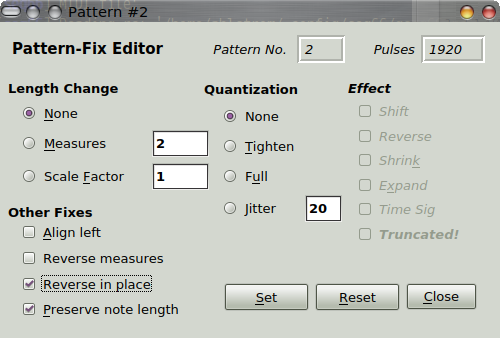
\includegraphics[scale=0.65]{pattern-editor/patternfix.png}
   \caption{Pattern Fix Dialog}
   \label{fig:pattern_editor_pattern_fix}
\end{figure}

   \index{pattern-editor!fix}
   When this dialog is used, the time-stamp of \textsl{every event} in the
   pattern will be changed.
   It is fairly intuitive to use.
   Once selected, the pattern number is shown in the title-bar and in a
   read-only text field.
   The \textbf{Length Change} selector allows for the following actions:

   \begin{itemize}
      \item \textbf{None}.
         No length change will occur.
         Alignment, reversing, and quantization can still be done.
      \item \textbf{Measures}.
         Allows the measures (length) of the pattern to be changed in two ways,
         depending on how the number is entered: as a simple integer (e.g.
         1, 1.0, 0.25),
         or as a simple time-signature fraction (e.g. "3/4").
         \begin{itemize}
            \item \textbf{Measures}.
               Entering an integer or a floating-point scale factor will scale
               the pattern events,
               and change the number of measures, if applicable.
               If the measure value is less than \texttt{1.0},
               the pattern will only be compressed.
               If less than 1 measure in length, the result will be
               1 measure; \textsl{Seq66} cannot allow less than 1 measure.
            \item \textbf{Time Signature}.
               Entering a fraction such as \textbf{3/4} or
               \textbf{12/8} will change the time signature of the pattern
               \textbf{and} \textsl{compress it to 1 measure}.
         \end{itemize}
      \item \textbf{Scale Factor}.
         Scales the pattern.  For example, 2.0 doubles the length, and 0.5
         halves the length.
         The \textbf{Measures} is changed to be enough to contain the new length,
         but only if the scale is greater than 1.0.
         One thing to be aware of is that, if the pattern is expanded, the
         new measure count depends on the location of the last event in the
         pattern. For instance, setting the scale factor to 100 might result in
         76 measures, not the 100 that would be set if measures was set to 100.
   \end{itemize}

   The \textbf{Quantization} selector allows for various types of
   quantization.
   It works the same as the \textbf{Tool} entries of the
   same name (see \sectionref{subsec:pattern_editor_second_row}),
   but works on \textsl{all events}, not just selected events.
   Also included is a \textbf{Jitter} option, with a range for the jitter.
   This option slightly randomizes the time-stamps of note events.

   \textbf{Other Fixes} provides some minor items, as follows.

   \begin{itemize}
      \item \textbf{Align left}
         allows the pattern to be aligned to the left of the sequence, removing
         any delays.  This is useful when recording a pattern live and not quite
         hitting the first beat in time.
      \item \textbf{Preserve note length}
         prevents Note Offs from being scaled, which would shorten or length the
         notes.
      \item \textbf{Reverse measures}
         reverses all of the events in the whole pattern, flipping the measures
         completely.  For example, if all the events occur near the end of the
         pattern, after reversal they will all appear near the beginning of the
         pattern.
      \item \textbf{Reverse in place}
         This is probably a more natural reversal method.
         The relative location of a cluster of notes doesn't change, but the
         notes are simply reversed in place.
   \end{itemize}

%  Question:  would a "pattern flip" (of the note values themselves) be useful?

   \textbf{Effect} does not do anything except show the effect of the changes.
   (Making it read-only might make it almost invisible in some themes.)
   Note the \textbf{Truncated!} check-box.  If checked, then
   the length of the pattern has reduced enough to drop some events.
   This only happens with the time-signature option.
   The process followed is:

   \begin{enumerate}
      \item Apply the left-alignment (if selected).
      \item Modify the number of measures (if selected).
      \item Do the scaling (if selected).
      \item Perform the quantization/tightening (if selected).
   \end{enumerate}

   Lastly, the effect of the change is shown, if applicable.
   Note that changing the measure in this dialog is different from
   changing the measures in the "length" dropdown, which only changes the
   measures.
   Changing the measures to a large number on a pattern of 1 measure will
   greatly expand the notes!

   Any accidental changes can be \textbf{Reset}
   in this dialog.
   Undo in the pattern-editor itself with \texttt{Ctrl-Z} affects
   only MIDI events, not things like changing time-signature from the
   drop-downs.

   \itempar{Follow Progress}{pattern editor!tools}
   This button toggles whether or not the progress bar follows
   progress in long patterns.  Turning off this feature is useful when
   one wants to concentrate on the current measure without the paging to
   subsequent measures that occurs with the "follow progess" feature.

   \itempar{Grid Snap}{pattern editor!grid snap}
   Grid snap selects where the notes will snap when
   \textsl{drawn} and when \textsl{moved} (but not when lengthened/shortenend).
   That is, it selects the snap-spacing for the notes
   The following values are supported:
   \textbf{1}, \textbf{1/2}, \textbf{1/4}, \textbf{1/8},
   \textbf{1/16} (\textsl{the default value}),
   \textbf{1/32}, \textbf{1/64}, and \textbf{1/128}.
   Additional values are also supported:
   \textbf{1/3}, \textbf{1/6}, \textbf{1/12}, \textbf{1/24},
   \textbf{1/48}, \textbf{1/96}, and \textbf{1/192}.
   The button to the left of this control resets it to the default value.

   \itempar{Note Length}{pattern editor!note length}
   Note length determines the duration of inserted notes.
   Like the \textbf{Grid Snap} values,
   the following values are supported:
   \textbf{1}, \textbf{1/2}, \textbf{1/4}, \textbf{1/8},
   \textbf{1/16} (\textsl{the default value}),
   \textbf{1/32}, \textbf{1/64}, and \textbf{1/128}.
   Additional values are also supported:
   \textbf{1/3}, \textbf{1/6}, \textbf{1/12}, \textbf{1/24},
   \textbf{1/48}, \textbf{1/96}, and \textbf{1/192}.
   The button to the left of this control resets it to the default value.

   \itempar{Zoom}{pattern editor!zoom}
   Horizontal zoom is the ratio between MIDI pixels and ticks, written as
   "pixels:ticks", where "ticks" is the "pulses" in "PPQN".
   For example, 1:4 = 4 ticks per pixel.
   Supported values are
   \textbf{1:1}, \textbf{1:2} (\textsl{the default value}),
   \textbf{1:4}, \textbf{1:8}, \textbf{1:16},
   and \textbf{1:32}, along with
   more values to support higher PPQN tunes:
   \textbf{1:64}, \textbf{1:128}, \textbf{1:256}, and \textbf{1:512}.
   The default zoom is 2 for the standard PPQN value, 192, but it
   increases for higher PPQN values, so that the default zoom looks sensible.
   As the right number (ticks) goes higher,
   the effect is to zoom out, and show more of the pattern.

   \itempar{Key of Sequence}{pattern editor!key}
   Selects the desired musical key for the pattern.  The following keys are
   supported:
   \textbf{C}, \textbf{C\#},
   \textbf{D}, \textbf{D\#},
   \textbf{E}, \textbf{F}, \textbf{F\#},
   \textbf{G}, \textbf{G\#},
   \textbf{A}, \textbf{A\#},
   and \textbf{B}.
   Changing the key shifts the marked note-rows
   for the \textbf{Musical Scale} setting and indicates the base notes
   of the key in a \textbf{bold} font.
   The small key button resets the key to \textbf{C}.

   \index{save musical key}
   The musical key that a sequence/pattern is set to is
   saved in the MIDI file along with the rest of the data for the sequence.
   \textbf{However},
   a change made to the key, scale,
   or background sequence (not to be confused with the background-recording
   sequence) in the pattern editor can be saved in the whole song,
   so that opening another sequence
   will apply the same settings to that sequence.  This is an optional feature,
   supported as noted below.
   Also see \textbf{Musical Scale} below for the scale-identification feature.

   \index{global-sequence}
   If the global-sequence feature is enabled, and the user selects
   a different key, scale, or background sequence in the pattern editor, 
   then \textsl{all} patterns share the selected key, scale, or background
   sequence.  Furthermore, these settings are saved in the "proprietary"
   section of the MIDI file, where they are available for all patterns.

   If the global-sequence feature is \textsl{not} enabled, and the user selects
   a different key, scale, or background sequence in the pattern editor, 
   then only that pattern will use the selected key, scale, or background.
   The key, scale, or background sequence change will be saved in the MIDI file
   only for that pattern, as a SeqSpec meta event.
   The global-sequence feature setting can be made in the 'usr' configuration
   file.

   \itempar{Musical Scale}{pattern editor!scale}
   Selects the desired background scale for the pattern; it provides a way for
   someone to key in notes that are only in that scale.
   When a scale is selected, the following features are supported:

   \begin{itemize}
      \item The notes that are \textsl{not}
         in the scale are shown as grey in the piano roll.
      \item For harmonic transposition, the notes are shifted
         so that they remain in the selected scale.
      \item The exact notes that are considered "in-scale" shift according
         to the value of the selected \textbf{Key of Sequence}.
   \end{itemize}

   \index{musical scales}
   The following musical scales are supported so far:

   \begin{itemize}
      \item \textbf{Off (Chromatic)}
      \item \textbf{Major (Ionian)}
      \item \textbf{Minor (Aeolian)}
      \item \textbf{Harmonic Minor}
      \item \textbf{Melodic Minor}
      \item \textbf{Whole Tone}
      \item \textbf{Blues}
      \item \textbf{Major Pentatonic}
      \item \textbf{Minor Pentatonic}
      \item \textbf{Phrygian}
      \item \textbf{Enigmatic}
   \end{itemize}

   Please let us know of any mistakes in these scales.
   Note that the \textbf{Melodic Minor} scale is supposed to
   descend in the same way as the natural \textbf{Minor} scale, but
   there is no way to support that trick in \textsl{Seq66}.

   One can select which \textbf{Musical Scale} and
   \textbf{Key} the piece is in nominally,
   and \textsl{Seq66} will grey those keys on the piano-roll that
   are \textsl{not} in the selected scale for the selected key.
   This is purely visual; a user can still add off-key notes.
   This feature makes it easier to stay in key while playing and recording.
   The scale will shift when a different \textbf{Key} is selected.

   \index{save musical scale}
   The scale that a pattern is set to is
   saved in the MIDI file along with the rest of the data for the pattern.
   A change made to the key, scale, or background pattern in
   the pattern editor can be saved globally, so that opening another pattern
   apply the same settings to that pattern.  This is a configurable feature in
   the 'usr' file; see "global\_seq\_feature".
   This option allows applying the key/scale/background-sequence
   either globally (all patterns) or locally (per-pattern), with each pattern
   holding its key, scale, and background-sequence settings in
   SeqSpec meta events.

   \index{scale identifier}
   \index{keys!ctrl-k}
   The pattern editor's piano roll has a little secret:
   the \textbf{Scale Identifier}.
   When the piano roll has focus and \texttt{Ctrl-K} is pressed,
   all of the notes in the pattern are analyzed to try to determine
   the both the key and the scale of the existing notes.
   The method is not sophisticated... the notes are counted and are matched
   against all of the keys (C to B) and scales supported by \textsl{Seq66}.
   The combinations with the highest number of notes are then shown in a
   message box.
   This simple analysis depends on having at least 8 notes in the pattern, and
   it is possible to get weird results if
   there are only a few \textsl{different}
   notes, as in a simple bass line.
   Don't expect miracles from this feature.
   A more sophisticated analysis, the
   \textsl{Krumhansl-Schmuckler} key-finding
   algorithm, could be used, but it is a bit too complex
   for our needs, which are basic.

   \itempar{Background Sequence}{pattern editor!background sequence}
   One can select another pattern to draw on the background to help with
   writing corresponding parts.
   The button brings up a small menu with values of \textbf{Off} and
   \textbf{Set 0} (at a minimum).
   The 0 is a set number; sets are numbered from 0 to 31.
   Additional set numbers appear in the menu for each set that has data in it.
   Under the \textbf{Set 0} entry, a menu appears.
   Once the desired pattern is selected from that list, it appears as dark cyan
   note bars, along with the normal notes that are part of the pattern.

   \index{save background sequence}
   The background sequence that shows is saved in the MIDI file
   along with the rest of the data for the sequence/pattern.
   A change made to the key, scale, or background sequence in
   the pattern editor is saved in the editor, so that opening another sequence
   will apply the same settings to that sequence.
   This is an optional feature, as noted earlier.

   \itempar{Chord Generation}{pattern editor!chord generation}
   One can insert chords with one click.
   (This feature comes from user "stazed"
   and his \textsl{Seq32} project \cite{seq32}.)
   Select the desired chord type first.
   Once a value other than \textbf{Off} is selected,
   drawing mode will add multiple notes representing the chord
   created, with the clicked note value as the base of the chord.

\subsection{Pattern Editor / Measures Ruler}
\label{subsec:pattern_editor_time}

   The measures ruler ("bar indicator", or "Time")
   consists of a \textsl{timeline} at the top and the 
   \textbf{L marker} and \textbf{R marker} items.
   The following are the elements next to and on
   the \textbf{Time} line:

   \begin{itemize}
      \item \textbf{Vertical Zoom Buttons}.
         These buttons allow the user to compress, reset, or expand the
         piano roll vertically to a certain degree.
         (The \texttt{v}, \texttt{V}, and \texttt{0} keys offer
         the same functions.)
         A more permanent change in vertical grid scaling
         can be made by setting the \textbf{Editor Key Height} value in
         the \textbf{Edit / Preferences / Display} tab,
         or in the 'usr' file.
      \item \textbf{Time Line}.
         The \textbf{Time} (or \textbf{Measures}) bar provides an explicit
         count of beats and bars.
         It follows the horizontal zoom of the piano roll.
         It also has a couple tricks, which are shown in the diagram below.
         \begin{itemize}
            \item \textbf{In the upper half} of the time-line,
               the mouse pointer changes to a vertical pointer.
               Clicking there then shows a vertical bar and a red dot; these mark
               the starting position of playback.
               This is useful for reviewing some notes.
            \item \textbf{In the lower half} of the time-line,
               the mouse pointer changes to a "finger" icon.
               Left-clicking there then moves the "L" marker to that point.
               Right-clicking there moves the "R" marker to that point.
               ("R" will never precede "L", though).
               If the \textbf{Loop} button in the main window is active, then
               playback will loop between the "L" and "R" buttons.
               This looping now works with both Live and Song modes.
         \end{itemize}
   \end{itemize}

   The following figure shows three steps in cursor movement, and the final
   result for setting a time-signature.

\begin{figure}[H]
   \centering 
   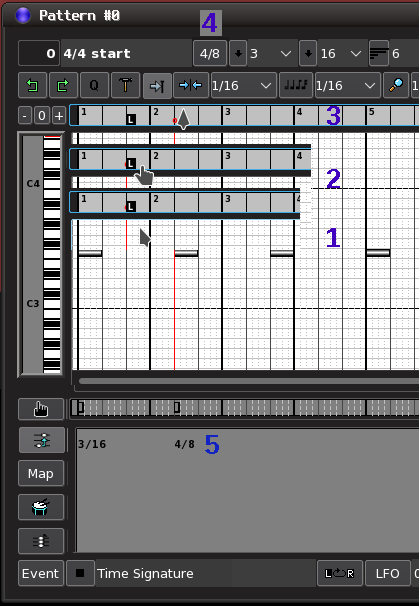
\includegraphics[scale=0.65]{pattern-editor/seqtime-cursor-composite.png}
   \caption{Setting a Time Signature}
   \label{fig:pattern_editor_seqtime_cursor_composite}
\end{figure}

   The steps shown are

   \begin{enumber}
      \item The mouse cursor is in the piano roll, and has the normal
         appearance for the current mouse cursor theme.
      \item The mouse cursor is in the bottom half of the time line, and
         here it's a pointing finger.
         When left-clicked, the "L" marker is set there.
         When right-clicked, the "R" marker is set there.
      \item The mouse cursor is in the top half of the time line, and is
         shown as a vertical arrow.
         A left- or right-click sets the current position in the
         pattern, and a red vertical line marks that position.
      \item The time-signature button (the "4/8" shown in the top
         bar) is clicked, and a time-signature is added at that point.
      \item The data pane switches to show Time Signatures.
         These cannot be edited in the data pane, but in the event bar above
         it, they can be selected by drawing a box around them, and then
         be either deleted or moved with the Left/Right arrow keys.
   \end{enumber}

   Note that the "L" and "R" markers can be selected via the keyboard using
   their respective shifted key.  Once selected, the marker can be moved left
   or right using the left and right arrow keys.
   Also note that the default position of the "R" marker is at the end of the
   fourth measure, so it might not be visible in the pattern editor without
   scrolling to it.

\subsection{Pattern Editor / Piano Roll}
\label{subsec:pattern_editor_piano_roll}

   The piano roll is the center of the pattern/loop/track/sequence editor.
   When a pattern is opened in the editor, the piano roll scrolls
   automatically to the first notes.

   The piano roll is accompanied by a thin "event bar"
   ("event pane") just below it,
   and a taller "data pane" or "data area" just below that.
   While the pattern editor is very similar to note editors in other
   sequencers, it is a bit different in feel.  A good mouse with at least 3
   buttons is very helpful for editing.  Buttons and keystrokes enhance the
   ease of editing.

   The piano roll shows notes, and, optionally, a background pattern or a
   scale.  Notes are shown as narrow rectanges; the background
   pattern and scale are shown as bars running the length of the piano roll.

   When the piano roll has keyboard focus, the \texttt{Space} key
   starts and stops playback, rewinding to the beginning when stopped.
   The \texttt{.} (period) key starts and pauses playback, without
   rewinding.
   The first \texttt{Esc} key stops playback;
   the second \texttt{Esc} key exits "paint" mode; and
   the third \texttt{Esc} key closes the pattern editor \textsl{if}
   the 'usr' \texttt{[pattern-editor] escape-pattern} option is set.
   This functionality is similar to that of the main window, but
   these keys are not reconfigurable in the piano roll.

   One can page vertically in the piano roll using the
   \index{keys!page-up} \texttt{Page Up} and 
   \index{keys!page-down} \texttt{Page Down} keys.
   One can go to the leftmost position using the 
   \index{keys!ctrl-home} \texttt{Ctrl-Home} key,
   and to the rightmost position using the
   \index{keys!ctrl-end} \texttt{Ctrl-End} key,
   The mouse scroll wheel can also be used to move the panes around.
   For implementation reasons, the scroll wheel is active
   \textsl{only} in the piano roll.

   \index{keys!arrows}
   \textsl{If no notes are selected}, the arrow keys will move the piano row
   up, down, left, and right in small steps.
   Otherwise, the selected notes are moved
   up, down, left, and right.

   \index{keys!hjkl}
   In addition, the "vi" keys \texttt{h}, \texttt{j}, \texttt{k}, and
   \texttt{l} will act like the arrow keys. This can be convenient, especially
   if the arrow-keys are unwieldly.  For example, the
   \textsl{Microsoft Arc} keyboard puts all four arrows on one button!

   \index{keys!ctrl-arrows}
   \textsl{If no notes are selected}, then \texttt{Ctrl-Left-Arrow}
   and \texttt{Ctrl-Right-Arrow} will move the progress bar to the left or
   right by one snap value.

   \index{step}
   \index{note step}
   With the note-step feature, if one paints notes with the mouse,
   the note position advances with each click.
   If one paints notes via an external MIDI keyboard, the notes are painted and
   the note position advances.
   To preview notes entered via a MIDI device, click the
   \textbf{MIDI Thru} button to activate so that they will be
   passed to the sound generator or software synthesizer.

\subsubsection{Pattern Editor / Piano Roll Items}
\label{subsubsec:pattern_editor_piano_roll_items}

   The center of the pattern editor consists of a time panel at the top,
   a virtual keyboard at the left, a note grid, a vertical scrollbar, an event
   panel, and a data panel at the bottom.

   \begin{enumber}
      \item \textbf{Beat}
      \item \textbf{Measure}
      \item \textbf{Virtual Piano Keyboard}
      \item \textbf{Notes}
   \end{enumber}

   \setcounter{ItemCounter}{0}      % Reset the ItemCounter for this list.

   \itempar{Beat}{piano roll!beat}
   The light vertical lines represent the beats defined by the configuration
   for the pattern.  The even lighter dotted lines between the beats are useful
   for snapping notes.

   \itempar{Measure}{piano roll!measure}
   The heavy vertical lines represent the measures (bars) defined by the
   configuration for the pattern.
   \index{pattern!end marker}
   Also note that the end of the pattern
   occurs at the end of a measure, and is marked by a blocky \textbf{END}
   marker.

   \itempar{Virtual Piano Keyboard}{piano roll!virtual piano keyboard}
   The virtual keyboard is a fairly powerful interface.  It shows,
   by shadowing, which note on the keyboard will be drawn. It can be
   played with a mouse, using left-clicks, to preview a short motif.
   Every octave, a note letter and octave number are shown, as in
   "C4".  If there is a difference scale in force, then the letter changes to
   match, as in "F\#5".

   \index{virtual keyboard!right-click}
   A right-click in the virtual keyboard area toggles the display
   between octave-note letters, MIDI note-numbers, and other views.
   The following figure shows all views, superimposed for comparison.

\begin{figure}[H]
   \centering 
   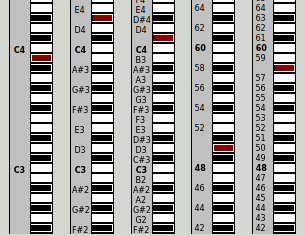
\includegraphics[scale=1.00]{pattern-editor/pattern-edit-window-key-numbers.png}
   \caption{Virtual Keyboard Number and Note Views}
   \label{fig:pattern_editor_key_numbers}
\end{figure}

   \itempar{Notes}{piano roll!notes}
   Musical notes are indicated in the piano roll
   by thick horizontal bars with white
   centers.  Each bar provides
   a visual representation of the pitch of a note and the length of a note.
   The current scale and background pattern can also be shown in the piano
   roll.

   \itempar{Time Scroll}{pattern editor!time scroll}
   Allows one to pan through the whole pattern, if it is too long to fit in
   the window horizontally.

\subsubsection{Pattern Editor / Note Painting}
\label{subsubsec:pattern_editor_note_painting}

   When we say "editing" in the context of the piano roll, in part we mean that
   we will "draw"
   \index{draw mode}
   \index{mode!draw}
   \index{paint mode}
   \index{mode!paint}
   or "paint" notes.
   Drawing, modifying, copying, and deleting notes is fairly easy in
   \textsl{Seq66}, though slightly different from other MIDI sequencers.

   The \textsl{Seq24} note-editing style is as expected for basic
   actions such as selecting and moving notes using the left mouse button.
   Drawing a note or event is a bit different, in that one must first
   enter the drawing mode ("paint mode").
   One way is to \textsl{click and hold} the right mouse button, and then
   \textsl{click and drag} the mouse to insert notes.
   (Note that one can use the \textsl{Ctrl-left-click} as a middle click. )
   \index{keys!p}
   Another way is to use the \texttt{p} key to enter the "paint" mode.
   To get out of the "paint" mode, press the
   \index{keys!x}
   \index{keys!Esc}
   \texttt{x} key while in the sequence editor.
   The \texttt{Esc} key also exits paint mode if the tune is not playing.
   Also available is a "finger" button
   (\textbf{Note Select/Note Entry})
   to click to toggle the mode.

   \index{notes!inserting}
   Notes are inserted to be at the current length and grid-snap values for
   the sequence editor for as long as the buttons are pressed while the mouse
   is dragged.
   The length of the note will
   be that specified in the note-length setting (e.g. "1/16").
   \index{auto-note}
   This is the "auto-note" feature.
   The auto-note feature also works with chord-generation.
   Notes are inserted only up to the specified sequence length.
   Once notes are inserted, moving the mouse with the left button still
   held down moves the notes to the new note value of the mouse.
   If one releases the left button, then presses and holds it again,
   more notes will be added in the same way.
   This is a good way to layer notes in a short sequence.
   The draw mode has the following features:

   \begin{itemize}
      \item Notes are continually added as the mouse is dragged ("auto-notes").
      \item Notes cannot be added past the "END" marker of the pattern, which
         marks the \textbf{Sequence Length in bars} setting.
      \item As the mouse is dragged while the left button is held in draw mode,
         notes are either added, or, if already present at that note-on time,
         are moved up and down.
      \item If the draw mode is exited, and entered again, then the original
         notes will not be altered.  Instead, new ones will be added.
      \item Notes can be added while the pattern is playing, and will be heard
         the next time the progress bar passes over them.
   \end{itemize}

   Drawing/painting can also be done while the sequence is playing,
   and notes will be added to be played the next time the progress bar crosses
   them.

\subsubsection{Pattern Editor / Note Editing}
\label{subsubsec:pattern_editor_note_editing}

   Once notes are in place, whether by recording or using "paint" mode,
   the piano roll provides a sophisticated set of note-editing
   actions.
   But, before editing, one can turn on
   \index{note!tooltips}
   "note tooltips", if desired.
   The thin button, labelled in tiny text as "Note Tips"
   next to the horizontal scroll bar toggles this mode.
   When enable, moving the mouse over a note will show its value, time range
   in units of B:B:T, and its velocity.
   This view is quicker than opening up the \textbf{Event Editor}.
   Onward!

   \setcounter{ItemCounter}{0}      % Reset the ItemCounter for this list.

   \itempar{Event Selection}{event!select}
   There are various ways to select events and copy, delete, or modify them
   using the mouse or the keyboard in the piano roll:

   \begin{itemize}
      \item
         \index{keys!ctrl-a}
         \index{selection!all}
         \textbf{\texttt{Ctrl-A}}.
         Pressing the \texttt{Ctrl-A} key will select all of the events in the
         pattern editor.
      \item
         \index{keys!ctrl-e}
         \index{selection!events by channel}
         \textbf{\texttt{Ctrl-E}}.
         Pressing the \texttt{Ctrl-E} key will select all of the events in the
         pattern editor that have the channel that is selected in the
         channel dropdown.
         This selection is useful if one wants to move events from one channel
         into another pattern.
      \item
         \index{keys!ctrl-n}
         \index{selection!notes by channel}
         \textbf{\texttt{Ctrl-N}}.
         Pressing the \texttt{Ctrl-N} key will select all of the notes
         in the pattern editor that have the channel that is selected in the
         channel dropdown.
         This selection is useful if one wants to move notes from one channel
         into another pattern.
      \item
         \index{mouse!left-click}
         \index{pattern editor!left click}
         \index{pattern editor!select note}
         \textbf{Left Click}.
         Pressing the left button on a note or a event deselects all other
         notes or events, and selects the item clicked on.
         The selected note will turn orange (or the configured palette color).
      \item
         \index{mouse!left-click-drag}
         \index{pattern editor!select multiple notes}
         \textbf{Left Click Drag}.
         Pressing the left mouse button and dragging also lets one
         select ("lasso") multiple events and notes.
         The selected notes will turn orange.
         Adjustments can be made to one or more notes by selecting one or more
         notes, and then applying one or more special
         \index{selection action}
         "selection actions" to the selection.
         Be careful!  If you \texttt{Ctrl-left-click-drag}
         on an already-selected note,
         the drag will change the length of
         \textsl{all of the notes in the selection}.
      \item \index{mouse!ctrl-left-click}
         \textbf{Ctrl Left Click}.
         Pressing the \texttt{Ctrl} key and the left button on a note or an
         unselected event \textsl{adds} that event to the selection.
      \item
         \index{pattern editor!transpose notes}
         \textbf{Left Click Drag Selection Up/Down}.
         To move notes in pitch, once selected, grab one of the notes in the
         selection and drag it upward or downward.
         \index{down arrow}
         \index{up arrow}
         Also, when a selection is in force, the
         \texttt{Up} and \texttt{Down} arrow keys will
         change the pitch of every note in the selection.
         The smallest unit of pitch change is one MIDI note value.
      \item
         \index{pattern editor!move notes in time}
         \textbf{Left Click Drag Selection Left/Right}.
         To move notes in time, once selected, grab one of the notes in the
         selection and drag it leftward or rightward.
         \index{left arrow}
         \index{right arrow}
         Also, since a selection is in force, the
         \texttt{Left} and \texttt{Right} arrow keys can also
         be used to change the time of every note in the selection.
         The smallest unit of time change is the \textbf{Grid snap} value,
         which might be a 16th note, for example.
      \item
         \index{mouse!ctrl-left-click-drag}
         \textbf{Ctrl Left Click Drag}.
         \begin{itemize}
            \item Pressing the \texttt{Ctrl} while left-click-dragging
               \textsl{on unselected events} lets one make additional
               selections of multiple events and notes.
            \item Pressing the \texttt{Ctrl} while left-click-dragging
               \textsl{on an already-selected event} lets one stretch or
               compress the lengths of all notes in the selection.
%              Also achievable via a \textbf{Middle Click Drag}.
               \index{pattern editor!event stretch}
               \index{event!stretch}
               \index{pattern editor!event compression}
               \index{event!compression}
               This feature is called \textsl{event stretch}
               or \textsl{event compression}.
               Notes can be shortened below the default note length by event
               compression.  There is currently no way to change the length of
               the note using a keystroke.
         \end{itemize}
      \item \index{pattern editor!deselect notes} \index{selection!deselect}
         \textbf{Deselect Notes}
   \end{itemize}

   \index{note!selection box}
   The selection, copying, and pasting of notes has some minor tricks to
   remember.  When some notes are selected, the effective selection box
   goes from the first note to the last note, and from the top-most note to the
   bottom-most note.
   When pasting the notes, place the mouse cursor so that it lies on the
   desired row for the top-most note, and on the desired time location for the
   left-most note.  After pasting, be sure to verify the notes in the new
   location.

   \index{warning!wrap-around notes}
   \textbf{Warning}:  Reducing or increasing the length of a note selection
   by too much causes the note or notes to "wrap-around" to the end
   of the pattern boundary and grow more from the beginning of the sequence. 
   If it happens, one probably ought to undo it.

   The \textbf{Tools} button described in
   \sectionref{subsec:pattern_editor_second_row} can also be used to
   modify selections.
   Once one or more notes are selected, they can be modified in time,
   pitch, or length, as described above.

   \textbf{Warning:}
   \index{warning!down arrow}
   \index{warning!up arrow}
   \index{warning!note loss}
   If one moves the selection too low or too high in pitch, whether with the
   mouse or the arrow keys, any notes that go below the lowest MIDI pitch or
   above the highest MIDI pitch \textbf{will be lost}!
   If done using the mouse, the undo feature (\texttt{Ctrl-Z}) will work.
   If done using the arrow keys, the undo feature does not work!
   Be careful, especially if you have a fast keyboard repeat rate!

   Note that there is no possibility of note loss with a change in time.  When
   a note disappears at one end of the pattern boundary, it wraps around to the
   other end.  Cool.

   \itempar{Copy/Paste}{pattern editor!copy/paste}
   Copying, cutting, and pasting is supported by selecting a number of events
   or notes, and using the
   \index{pattern editor!cut}
   \index{keys!ctrl-x} Cut (\texttt{Ctrl-X}), 
   \index{pattern editor!copy}
   \index{keys!ctrl-c} Copy (\texttt{Ctrl-C}), and
   \index{pattern editor!paste}
   \index{keys!ctrl-v} Paste (\texttt{Ctrl-V})
   keys.
   When the notes are selected,
   \index{pattern editor!delete}
   \index{keys!del}
   \index{keys!backspace}
   one can delete them with the \texttt{Delete} or \texttt{Backspace} key.
   If the events are \textsl{cut}, using the \texttt{Ctrl-X} key, then
   they can be pasted, using the \texttt{Ctrl-V} key, then
   moving the cursor to the desired place, and clicking.

   One can move the selection box using the arrow keys, to the
   desired location, and then click to
   drop the notes at that location.
   Selected notes that are cut or copied can also be
   pasted into \textsl{other} pattern editor dialogs; that is, they can be
   pasted into other sequences.

\subsubsection{Pattern Editor / Other Keys}
\label{subsubsec:pattern_editor_other_keys}

   Here are some other, less standard,` keys useful in the pattern editor piano roll:

   \begin{itemize}
      \item
         \index{keys!c}
         \index{selection!repitch}
         \textbf{\texttt{c}}.
         Pressing the \texttt{c} key will attempt to use the note-mapper data
         (provided by a \texttt{*.drums} file) to change the notes in the
         pattern.  This will work only if the pattern is marked as transposable,
         to add some safety against multiple pitch changes; these are useful once
         when converting from one drum machine to General MIDI.
      \item
         \index{keys!ctrl-d}
         \index{selection!clear}
         \textbf{\texttt{Ctrl-D}}.
         Pressing the \texttt{Ctrl-D} key will clear the pattern clipboard.
      \item
         \index{keys!f}
         \index{selection!edge fix}
         \textbf{\texttt{f}}.
         Pressing the \texttt{f} key will attempt to fix wrap-around notes by
         moving the note.
      \item
         \index{keys!ctrl-k}
         \index{selection!analyze}
         \textbf{\texttt{Ctrl-k}}.
         Pressing the \texttt{Ctrl-k} key will analyze all the notes in the
         pattern to try to guess its scale, as discussed earlier.
      \item
         \index{keys!o}
         \index{recording toggle}
         \textbf{\texttt{q}}.
         Pressing the \texttt{o} key will toggle recording for the pattern.
      \item
         \index{keys!q}
         \index{selection!quantize}
         \textbf{\texttt{q}}.
         Pressing the \texttt{q} key will quantize the selected notes.
      \item
         \index{keys!r}
         \index{selection!randomize}
         \textbf{\texttt{r}}.
         Pressing the \texttt{r} key will quantize the selected notes.
      \item
         \index{keys!t}
         \index{selection!tighten}
         \textbf{\texttt{t}}.
         Pressing the \texttt{t} key will partially quantize (tighten)
         the selected notes.
      \item
         \index{keys!u}
         \index{selection!remove unlinked notes}
         \textbf{\texttt{u}}.
         Unlinked notes no longer occur.  But....
%        Unlinked notes do not occur unless note-wrap-around occurs.
%        When they do occur, they are painted in magenta.
         Pressing the \texttt{u} key will remove any unlinked notes found in
         the pattern.
         This fix is a stop-gap until we can figure out
         the best way to prevent unlinked notes while handling recording of
         notes near the end of the pattern length.
      \item
         \index{keys!=}
         \index{selection!relink notes}
         \textbf{\texttt{=}}.
         Pressing the \texttt{=} key relinks any unlinked notes found in
         the pattern. This causes the notes that are unlinked to be linked, and
         thus wrap around.
      \item
         \index{keys!space (play)}
         The default keystroke for starting playback is the \texttt{Space}
         character.
      \item
         \index{keys!esc (stop)}
         The default keystroke for stopping playback is the \texttt{Escape}
         character.
      \item
         \index{keys!period (pause)}
         The default keystroke for pausing playback is the \texttt{Period}
         character.
   \end{itemize}

\subsubsection{Pattern Editor / Zoom Keys}
\label{subsubsec:pattern_editor_zoom_keys}

   \index{zoom keys}
   \index{keys!0}
   \index{keys!z}
   \index{keys!shift-z}
   After a left-click in the piano roll, the
   \textbf{z}, \textbf{Z}, and \textbf{0}
   can be used to zoom the piano-roll view \textsl{horizontally}.
   The \textbf{z} key zooms out (smaller),
   the \textbf{Z} key zooms in (larger),
   and the \textbf{0} key resets the zoom to the default value.
   The horizontal zoom feature also affects the time-line
   (measures indicator) and the data area.

   \index{keys!v}
   \index{keys!shift-v}
   The note display can also be zoomed vertically.
   The \textbf{v} key zooms out vertically to make the notes thinner,
   the \textbf{V} key zooms in vertically to make the notes fatter,
   and the \textbf{0} key resets the zoom to the value of the "key height"
   setting in the 'usr' configuration file.
   
\subsection{Events Pane}
\label{subsec:pattern_editor_panel}

   Also known as the "events pane" or "events editor".
   The narrow (a few pixels high) events strip shows discrete events,
   such as \texttt{Note On} and \texttt{Note Off}.
   The events that are shown are selectable in the \textbf{Event} category
   selector and the "Selector for Existing Data"" drop-downs at bottom left.
   \index{event strip}
   These and other events appear
   as small squares in the event strip, along with a black vertical bar
   in the \textbf{Data Pane} with a
   height proportional to the data-value of the event and a numeric
   representation of that value.
	The event value (data) editor (directly under the event strip) is used 
	to change note velocities, channel pressure, control codes,
	patch select, etc.

   \textsl{We currently recommend being careful of editing or selecting events
   in that pane (feel free to disobey)}.
   Note On and Note Off events cannot be inserted in the event strip;
   it is too easy to screw up.
   Selection and editing in the events pane is disabled for
   \textbf{Note On}, \textbf{Note Off}, and \textbf{Aftertouch}.

   \index{events!insert}
   Other event types (including tempo) can be inserted via the event strip.
   To do that, first select the kind of event to insert using the
   \textbf{Event} button in the bottom panel; this process won't work
   for Note events.
   Then place the mouse cursor in the event strip and click to give it
   focus.
   Do one of the following:

   \begin{itemize}
      \item Right-click to make the drawing cursor appear at
         the exact spot where the event must go.  While holding the right
         button, click the left button.
         A small square for the event will appear.
         Or click-drag to insert a
         series of events, each at a snap value.
      \item Or press \texttt{i} (insert) or \texttt{p} (paint).
         to make the drawing cursor appear.
         Then click the left button or drag to paint as above.
   \end{itemize}

   Drawing mode can be exited by releasing the right mouse button or
   by pressing \texttt{Esc} or \texttt{x} (exit).

   \textsl{Note: we might, in the future, repurpose \texttt{p} and
   \texttt{x} for more obvious operations.}

   Note that the "finger" button \textsl{does not} apply to the event panel;
   it applies only to inserting notes in the piano-roll.

   \textsl{Be careful}
   when using smaller snap values (1/32, 1/64, etc.) to insert events.
   Move the mouse cursor very slowly, otherwise some snap values might be
   skipped, leaving missing events.  In that case, either remove the events and
   try again, or use the event editor to add events at the missing tick
   positions.

   To move the event(s) to a different time, select it/them via the left
   button.  Then drag the selection left or right as desired.
   The left and right arrow keys can also be used.
   \index{todo!high precision events}
   it is currently not possible to move them to positions smaller than the
   beat size; temporarily reduce the beat size if desired.
   Also, for regularly-spaced events, selected events can be hidden when moved
   into the next non-selected event.
   The event values can be edited via the data panel, described in the next
   section.

\subsection{Left Buttons}
\label{subsec:pattern_editor_left_buttons}

   Once the events are in place, the next step is to modify the
   data values of the events as needed.
   But first, note the buttons at the left.

   \begin{enumber}
      \item \textbf{Transpose}
      \item \textbf{Note Map}
      \item \textbf{Drum Note Mode}
      \item \textbf{Chord Generation Reset}
   \end{enumber}

   \setcounter{ItemCounter}{0}      % Reset the ItemCounter for this list.

   \itempar{Transpose}{pattern editor!transpose toggle}
   This button toggles the ability of the sequence to be transposed.
   If transpose is enabled for that pattern, the button will be highlighted as
   per the current desktop theme.  Patterns for drums should, in general, not
   be transposable.

   \itempar{Note Map}{pattern editor!note map}
   If the pattern is transposable, then this button is enabled.
   If clicked, it applies the note-mapper to all of the notes in the pattern.
   See \sectionref{subsec:configuration_drums}.
   It is most useful for converting percussion from older drum sets to
   General MIDI drums.  Enable transposition, apply the mapping, and then
   disable transposition to avoid transposing again (e.g. by accident).

   \itempar{Drum Note Mode}{pattern editor!drum mode}
   This button changes from normal note mode to drum note mode. In the drum
   mode, the notes are drawn as small red diamonds without any duration.
   They are also entered the same way.
   This is a feature adopted from \textsl{Kepler34}.

   \itempar{Chord Generation}{pattern editor!chord generation}
   \index{chord generation}
   This button resets the chord-generation feature to \textbf{Off}.
   It's located by the data pane in order to save space in the first row.

\subsection{Data Pane}
\label{subsec:pattern_editor_data_view}

   Now on to the \textbf{Data Pane} itself, also known as the "data panel".
   The events that are shown in this pane
   are selectable in the \textbf{Event} category
   selector and the "Selector for Existing Data"" drop-downs at bottom left.
   \index{data pane}
   \textbf{Modify Event Data} offers a way to
   alter the event data values.
   Many different events can be altered in the data pane:
   Note On and Note Off velocities, program changes, aftertouch, channel
   pressure, pitch wheel, and tempo.
   Text events are also displayed (useful in karaoke), but they cannot be
   edited in this pane
   (instead see the \textbf{Session} tab's \textbf{Song Info} controls and
   the \textbf{Event Editor}.).

   The events values for the currently selected category of events are shown
   in this window as vertical lines of a height proportional to the value,
   \index{data!grab handle}
   topped by a circular grab handle.
   The exceptions are program changes and tempo, which are shown by small
   circles, yellow in the case of tempo.
   Also, the range of tempos in the data panel is set to match the
   \index{usr!bpm-minimum}
   \texttt{usr!bpm-minimum}
   and
   \index{usr!bpm-maximum}
   \texttt{usr!bpm-maximum}
   settings in the 'usr' file.
   This range is for display purposes.
   See \sectionref{subsubsec:usr_file_user_midi_settings}.

   These values can be easily modified by
   \index{mouse!left-click-drag}
   left-click-dragging the
   mouse past each line, to level it off at the given value.
   Easier to try it than explain it.
   \index{mouse!right-click-drag}
   Right-click-drag also works the same.
   \index{modify event-data}
   When notes are \textsl{selected}, and the
   mouse is used to change the values (heights) of the lines in the event-data
   area, \textsl{only the events that are selected} are changed.
   The data-values of \textsl{unselected} events are left unchanged.
   A cool feature from \textsl{Seq24}.

   Also, as the mouse passes over the data pane, events near the mouse
   acquire a grab handle, which can be used to select the event
   and modify its value by moving the mouse up or down.

   Note that some events are shown as small circles instead of a line; each
   circle has the numeric value next to it.

   \textbf{Tempo}
   events are shown as a small yellow circle.
   This circle can be grabbed and moved up or down.

\begin{figure}[H]
   \centering 
   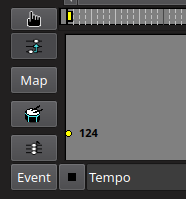
\includegraphics[scale=1.0]{pattern-editor/data-pane-tempo.png}
   \caption{Data Pane Tempo}
   \label{fig:pattern_editor_data_pane_tempo}
\end{figure}

   A new feature is the ability to
   add tempo events in the data pane.
   To add a string of tempo events, first select \textbf{Tempo}
   from the \textbf{Event} dropdown.
   Move to the data pane, press and hold \texttt{Ctrl}
   and then left-click-drag the mouse to form a line
   as shown here.

\begin{figure}[H]
   \centering 
   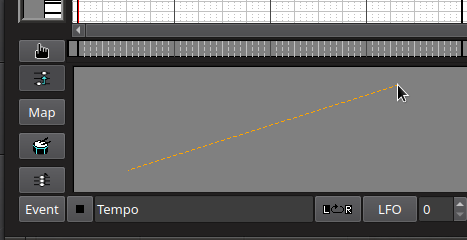
\includegraphics[scale=1.0]{pattern-editor/data-pane-tempo-0.png}
   \caption{Data Pane Tempo Line Draw}
   \label{fig:pattern_editor_data_pane_tempo_line_draw}
\end{figure}

   Note that there are no events shown yet.
   While still holding \texttt{Ctrl}, release the left mouse button,
   and the tempo events appear.
   Release the \texttt{Ctrl} key.
   If this line of tempos is fine, right-click to lock them.

\begin{figure}[H]
   \centering 
   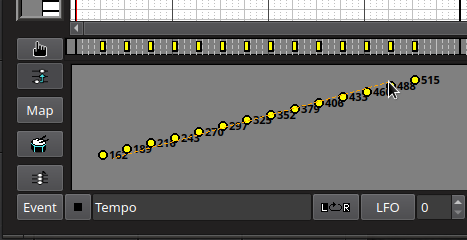
\includegraphics[scale=1.0]{pattern-editor/data-pane-tempo-1.png}
   \caption{Data Pane Tempo Events Drawn}
   \label{fig:pattern_editor_data_pane_tempo_events_drawn}
\end{figure}

   Otherwise, move the mouse around to change
   the tempo events, as shown here.
   Use the right-click to exit this mode.

\begin{figure}[H]
   \centering 
   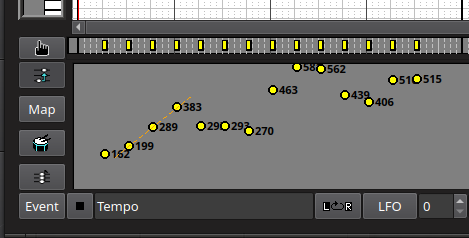
\includegraphics[scale=1.0]{pattern-editor/data-pane-tempo-2.png}
   \caption{Data Pane Tempo Events Altered}
   \label{fig:pattern_editor_data_pane_tempo_events_altered}
\end{figure}

   Again, note that the range of the tempo events is
   determined by the BPM minimum and maximum values
   specified in the 'usr' file.
   There is currently no \textbf{Preferences}
   setting for these values.  

   Also note that, to delete tempo events in the pattern editor,
   select the events in the thin event pane, then press
   either \texttt{Delete} or \texttt{Ctrl-X}.
   They can also be deleted (slowly) in the event editor.

   \textbf{Program Change}
   events are shown as a small open circle with a numeric value.
   Both Tempo and Program Change event values can be modified by dragging a
   line as discussed above. (We're still working on select-and-drag for
   these events.)

\begin{figure}[H]
   \centering 
   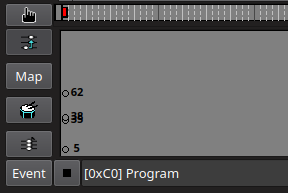
\includegraphics[scale=1.0]{pattern-editor/data-pane-program.png}
   \caption{Data Pane Program Change}
   \label{fig:pattern_editor_data_pane_program_change}
\end{figure}

   As of version 0.99.9, we have added \textsl{Seq32}-style grab-handles
   to the Note events in the data panel.
   They are shown only if an event is selected, or if the mouse
   is on top of the event line.
   As the mouse moves through the data panel, the grab-handles are shown
   as circles at the top of each line.
   If the line is clicked, it is selected.
   If Ctrl-clicked, the selected line is added to the selection.
   If an empty spot in the data pane is clicked, all events are
   unselected.
   When present, the circular grab-handle can be clicked-and-held
   and moved up and down to change the event value.

\begin{figure}[H]
   \centering 
   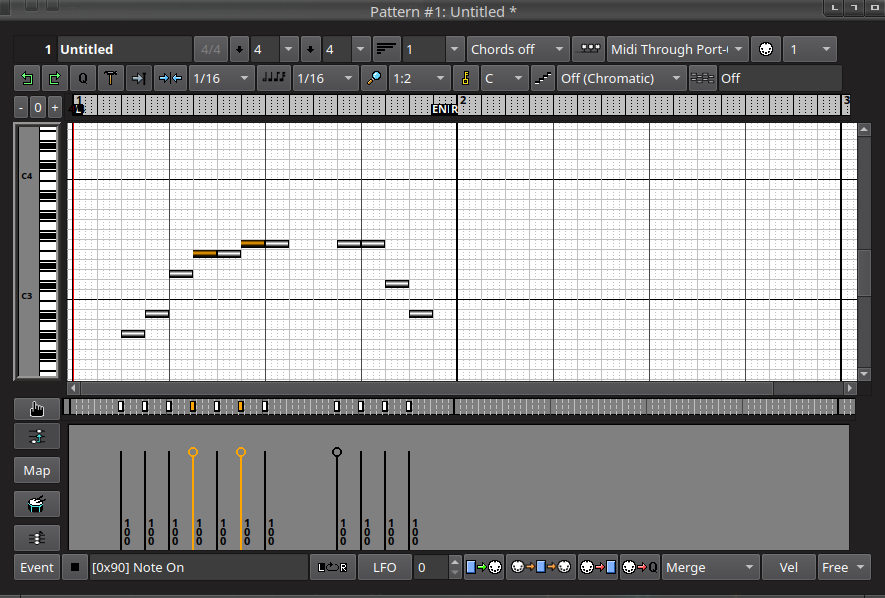
\includegraphics[scale=1.0]{pattern-editor/grab-handles.png}
   \caption{Data Pane Note Grab-Handles}
   \label{fig:pattern_editor_data_pane_note_grab_handles}
\end{figure}

   \index{event data editor!mouse wheel}
   Any events that are selected in the piano roll or event strip can have
   their values modified with the mouse wheel.
   Data values can also be modified using the \textbf{LFO} pane (see below).

\subsection{Pattern Editor / Bottom Row}
\label{subsec:pattern_editor_bottom}

   The bottom row of the pattern editor provides for
   selecting events for viewing and editing, MIDI playback,
   pass-through, and recording.

   \begin{enumber}
      \item \textbf{Event Category Selector}
      \item \textbf{Selector for Existing Data}
      \item \textbf{Selected Event Name}
      \item \textbf{LFO Panel}
      \item \textbf{Live Loop Count}
      \item \textbf{Armed/Muted Toggle} (Data To MIDI Buss)
      \item \textbf{MIDI Thru Toggle}
      \item \textbf{MIDI Record Toggle}
      \item \textbf{MIDI Record Quantized}
      \item \textbf{Loop Record Type} (Overdub, Replace, Expand, One-shot)
      \item \textbf{Record Velocity and Reset}
   \end{enumber}

   \setcounter{ItemCounter}{0}      % Reset the ItemCounter for this list.

   \itempar{Event Category Selector}{pattern editor!event selector}
   This button brings up the following context menu, so that the user can
   select the category of events to view and edit.

\begin{figure}[H]
   \centering 
   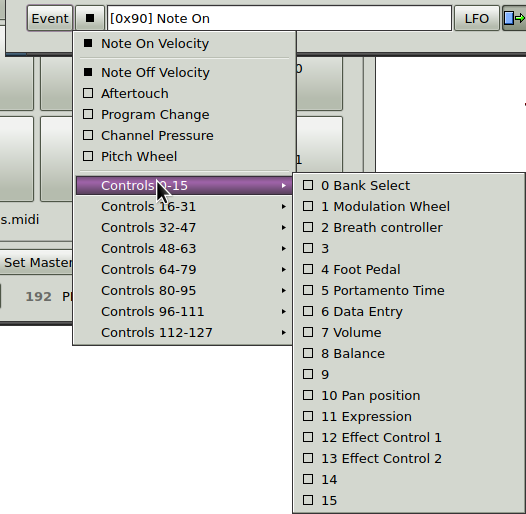
\includegraphics[scale=0.75]{pattern-editor/event-context-menu.png}
   \caption{Pattern Editor Event Button Context Menu}
   \label{fig:pattern_editor_bottom_event_context_menu}
\end{figure}

   Note the squares.  Some might be filled (black), most are empty.
   Filled squares indicate that the sequence has some events of that type.
   Otherwise, there are no such events in the sequence.
   Useful in deciding if it is worth selecting the event.

   The sub-menus of this context menu show 128 MIDI controller messages.
   They also use the squares to
   indicate if there are any events of the type shown in the menu.
   These sub-menus can be modified by editing the 'usr' file:
   
   \begin{verbatim}
      $HOME/.config/seq66/seq66.usr
   \end{verbatim}

   to make it match one's instrument.

   \itempar{Existing Event Menu}{pattern editor!existing events}
   The existing-event selector is a small button (with a black-square icon)
   that brings up a menu with only existing events shown.
   Unlike the event-selector described above, this menu
   shows only the actual events existing in the track, for quicker selection.

   \itempar{Event Selection}{pattern editor!event selection}
   Shows the selection event, with its event number shown in hexadecimal
   notation, and the name of the event shown.

   \itempar{LFO Panel}{pattern editor!LFO}
   An LFO (low-frequency oscillator) allows data events
   to be modulated by some rudimentary wave functions.
   By clicking on the \textbf{LFO} button or using the \texttt{Ctrl-L} key,
   the following window appears, with a set of 4 vertical sliders:

\begin{figure}[H]
   \centering 
  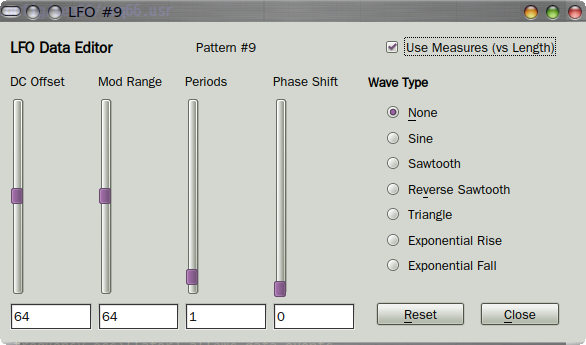
\includegraphics[scale=0.65]{pattern-editor/lfo.png}
   \caption{Pattern Editor LFO}
   \label{fig:pattern_editor_bottom_lfo}
\end{figure}

   \begin{enumber}
      \item \textbf{Use Measures (vs Length)}.
         The length of a waveform period can be determined by the length of the
         pattern (2 measures as shown next to the label "LFO Data Editor") or
         by the length of a measure. This check-box determines that.
         In the diagram, it is checked, so the 2 measures covers four periods
         of the sine wave.
         Especially useful in modifying long patterns.
      \item \textbf{DC Offset} (\textbf{D}).
         Provides a kind of DC offset for the data value. Starts at 64, and
         ranges from 0 to 127.
         In the diagram above, one can see that the 0-value line for the sine
         wave is at 64.
      \item \textbf{Depth} (\textbf{R}).
         Controls the depth of modulation.
         Starts at 64, and ranges from 1 to 127.
         The data values range from \( y = DC - R \) to \( y = DC + R\).
         For the sine-wave shown above, the range is 0 to 128 (actually 127).
      \item \textbf{Periods}.
         Indicates the number of periods per pattern length.
         For long patterns, this parameter should be set high,
         to even show an effect.  It is also subject to an 'anti-aliasing'
         effect, especially for short patterns.
         Try it!
      \item \textbf{Phase Shift} (\textbf{P}).
         Provides the phase shift within a period of the LFO wave.
         A value of 1 is a phase shift of 360 degrees (one whole period).
         Thus, the data at \( P = 0 \) would look exactly the same at phase
         \( P = 1\).
      \item \textbf{Wave Type}.
         Selects the kind of wave to use for the LFO:
         \begin{enumber}
            \item \textbf{None}.
               This setting is useful if one wants to change only the DC
               offset.
            \item \textbf{Sine}.
               Modulates via a sine wave.
               Change the \textbf{Phase Shift} to get a cosine function.
               If the \textbf{DC Offset} is below 64, then negative values are
               converted to positive. As an example, setting the DC offset to 0
               will produce the absolute value of the \texttt{sin()} function.
            \item \textbf{Sawtooth}.
               Provides a ramp modulation.
            \item \textbf{Reverse Sawtooth}.
               Provides a ramp modulation in the opposite direction.
            \item \textbf{Triangle}.
               Modulates via a triangle wave; somewhat similar to a sine wave.
            \item \textbf{Exponential Rise}.
               Provides an exponential ramp modulation.
               This ramping is easiest to see if the DC offset is 0,
               and the Mod range is 127.
               Varying the \textbf{Phase Shift} with the slider
               will move the peak of the curve left to right.
            \item \textbf{Exponential Fall}. Provides a ramp modulation in the
               opposite direction.
         \end{enumber}
         Note that one might have to change a parameter slightly to see the
         effect of the new waveform.
      \item \textbf{Reset Data}.
         This button restores the initial pattern event data.  Useful when one
         applies modulation that one ultimately does not like.
      \item \textbf{Close}.  Closes the LFO panel.
   \end{enumber}

   In addition to the \textbf{Reset Data} button, Ctrl-Z can be applied
   multiple times to undo changes one at a time.  Every motion of a control
   causes a complete change.

   \itempar{Live Loop Count}{pattern editor!live loop count}
   Normally, in Live mode, a pattern plays endlessly if left alone.
   If this counter is set to a value greater than 0, then the pattern will loop
   only that number of times in Live mode.  For example, if set to 1, then the
   pattern acts like a "one-shot" loop.  This can save having to use
   queuing quickly to handle an intro phrase.
   To loop \textsl{endlessly}, set this value to 0.
   Also set it to 0 when playing the MIDI tune in \textbf{Song} mode.
   Otherwise, weird behavior will be observed.

   \itempar{Armed/Mute Toggle}{pattern editor!data to midi buss}
   This button causes the pattern to be output to the
   selected MIDI output buss,
   which will normally be connected to a software or hardware
   synthesizer, to be heard.
   This item performs muting/unmuting (disarming/arming) in the same way a
   pressing the corresponding pattern button in the \textbf{Live} frame.

   \itempar{MIDI Thru Toggle}{pattern editor!midi data pass-through}
   This button routes incoming MIDI data through
   \textsl{Seq66}, which then writes it to the MIDI output buss.
   When a new pattern editor is opened,
   and the new-editor-editor settings
   (\sectionref{paragraph:user_file_added_options_pattern_editor})
   are false, one can click the
   \index{thru}
   \textbf{Thru} button first to redirect MIDI controller input
   to the synthesizer port, and have it be heard, without
   arming the pattern or turning on MIDI Record.
   Note, though, that if MIDI Record is toggled on and off, the
   Thru function is effectively disabled.  To restore it,
   toggle the Thru off, then on, again.
   Also note that Thru will remain enabled when the pattern editor is closed.

   \textsl{Warning:}
   If Thru is active, and the output port for the pattern is the
   same as the input port, then the struck note will be repeated
   for as long as recording is active.

   \itempar{MIDI Record Toggle}{pattern editor!record midi data}
   This button routes incoming MIDI data into
   \textsl{Seq66}, which then saves the data to the sequence, and also
   displays the new information (notes) in the piano roll view.
   Note that \textsl{Seq66}'s pattern grid can be put in various recording
   modes (e.g. overdub/merge versus overwrite) where, instead of
   muting/unmuting the patterns, it turns on recording (without opening the
   pattern editor).
   If expand-recording is active, this button shows double arrows, the
   second arrow indicating expandability.

   \itempar{MIDI Record Quantized}{pattern editor!quantized record}
   This button should be called "MIDI Record Altered", as it now supports
   more than just quantization.
   With every click, this button changes the type of alteration, cycling
   between these changes:

   \begin{enumber}
      \item \textbf{None}.
         No alteration of the recorded input is done.
         The button shows as unselected.
      \item \textbf{Tighten}.
         The recorded input will be lightly quantized.
      \item \textbf{Quantize}.
         The recorded input will be fully quantized.
         The quantization is to the current snap value.
      \item \textbf{Notemap}.
         If a note-map (see the 'drums' file) is loaded, the remapping of notes
         is applied on the fly.
   \end{enumber}

   Alteration can be turned on globally in \textsl{Seq66}'s pattern grid
   as well.
   When the pattern is opened, the alteration and recording style are
   set for that pattern.

   \textsl{Currently, changing the alteration and recording style in the grid
   changes the open pattern as well.  We are not sure if that is a good feature
   or not.}

   \itempar{Loop Record Type}{pattern editor!recording type}
   In \textsl{Seq24}, the pattern recording worked by merging new notes played
   as the pattern to be recorded was looped.  This method allows a loop to be
   built up bit-by-bit.  \textsl{Seq66} adds two more methods from
   Stazed's \textsl{Seq32} project.  The three methods are:

   \begin{enumber}
      \item \textbf{Overdub}.
         \index{merge}
         \index{overdub}
         \index{recording!merge}
         \index{recording!overdub}
         This is the normal style of recording loops, where notes can
         accumulate as the loop repeats.
%        See \sectionref{paragraph:patterns_recording_modes}
         Note that this item used to be called "Merge".
      \item \textbf{Overwrite.}
         \index{overwrite}
         \index{recording!overwrite}
         When the loop starts over, and a note is pressed,
         then the existing notes in that loop are erased,
         and the new note is added.
         This provides a good way of correcting major mistakes, live.
         It will not work if adding notes while not recording.
         This mode can cause incomplete notes if one
         holds the note and releases it in the next iteration, leaving a
         partially-drawn note behind.  The workaround is to try again.
      \item \textbf{Expand}.
         \index{expand}
         \index{recording!expand}
         Expansion operates when playing and recording.
         Once the end of the loop is near, when
         notes are being input, another measure is added to the length
         of the loop.
         This continues indefinitely, whenever any notes are
         being played and recorded.
         \index{recording!expand issue}
         This works best in \textbf{Live} mode.
         In \textbf{Song} mode, only one measure is added each time play is
         started, and playback stops when the song is complete.
         A workaround is to add a long track, perhaps empty, to the song.
         Awaiting user complaints to decide what to do.
      \item \textbf{Oneshot}.
         \index{oneshot}
         \index{recording!oneshot}
         When this option is set, with the record button on, and no pattern
         playing, recording won't start until a note comes in, and when the
         first note comes in, the progress bar starts at the left (time 0).
         As each new set of notes at the same timestamp come in, the
         notes are recorded and the current time advances by one snap value.
         The length of each note is determined by the snap size for the spacing
         of drawn events.
         At the end of the pattern, recording stops automatically.
         See the figure
         below for a recording from a \textsl{Yamaha DD-11}.
   \end{enumber}

   Remember that \textsl{Oneshot recording} is a kind of auto-step/step-edit
   recording, and that auto-step/step-edit can also be done by click-dragging
   the mouse.  Do not confuse it with \textsl{Oneshot playback}.

\begin{figure}[H]
   \centering 
   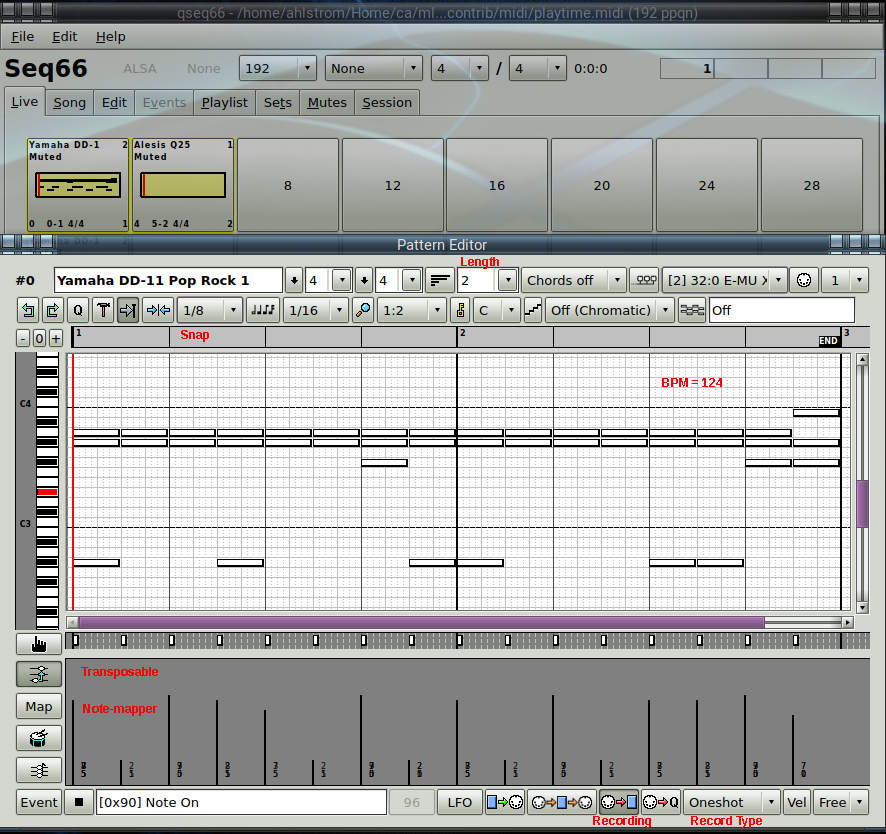
\includegraphics[scale=0.65]{pattern-editor/oneshot-recording.png}
   \caption{One-Shot Pattern Recording}
   \label{fig:pattern_editor_oneshot_recording}
\end{figure}

   In the figure above, we set up to record input from the port attached to a
   \textsl{Yamaha DD-11} drum machine.  After some trial and error,
   we set:

   \begin{itemize}
      \item \textbf{Length} to 2 measures (see the red text in the figure).
      \item \textbf{Snap} to 1/8th, which sets the spacing of drawn notes as
         well.  This determines the position of each new note.
      \item \textbf{Note Length} to 1/16th, which sets the length of drawn
         notes as well.
      \item \textbf{Recording Type} to \textbf{Oneshot}.
      \item \textbf{Recording} on. This is the button with the MIDI DIN
         connector pins going into the blue vertical rectangle.
   \end{itemize}

   Also, the \textbf{BPM} was set to 124 in the main
   window, to match the "39" tempo in the DD-11, which maps to 124 bpm.
   Finally, we picked the \textsl{Pop Rock 1} style.  
   Once this setup was in place, clicking the DD-11 Start/Stop button started
   recording automatically at time 0, and it stopped automatically at the
   length/end of the pattern.

   \index{auto-step}
   \index{step-edit}
   \index{recording!auto-step}
   \index{recording!step-edit}
   \index{auto-step!recording}
   \index{step-edit!recording}
   Why is the snap used instead of the note-length?  Because we're using the
   auto-step (step-edit) recording feature...
   the snap determines where the next note
   begins, and the length determines the length of the note to create.
   However, the note-length is a property of the piano roll, not the pattern
   itself.  The pattern uses the snap-length during auto-step/step-edit.
   This kind of note recording can be done in two ways:

   \begin{enumerate}
      \item Left-click-drag the mouse.
      \item Turn on recording without the pattern playing, then
         enter notes; recording stops when the end of the length is reached.
   \end{enumerate}

   Now, the DD-11 is an old instrument from the pre-General-MIDI days.
   So, in order to play back this pattern on something like
   \textsl{QSynth} or \textsl{Hydrogen}, we need to re-map the notes to GM drum
   notes.  In the 'rc' file, the proper note-mapper file is specified:

   \begin{verbatim}
      [note-mapper]
      "GM_DD-11.drums"
   \end{verbatim}

   We copy the recorded pattern and paste it into another slot for safety.
   We click the \textbf{Transposable} button for that pattern to enable the
   \textbf{Map} button.  Then we click the \textbf{Map} button, and the notes
   shift (not shown).  
   We click the \textbf{Transposable} button again to disable transposing,
   and save the file.
   Playing it into channel 10 of \textsl{QSynth} shows that it sounds a lot
   like the original DD-11 drums.

   \itempar{Vol}{pattern editor!vol}
   This button resets the volume (velocity)
   of note recording to the \textbf{Free} setting.
   See the next item.

   \itempar{Velocity}{pattern editor!velocity}
   This dropdown allows setting the volume of the recording to either the
   incoming velocity or to the specified velocity.
   The velocity values are shown at the right side of each menu entry.
   These values correspond to MIDI volume levels from 127 down to 16.
   If the \textbf{Free} item is selected, then the incoming note velocity is
   preserved.

\subsection{Pattern Editor / Common Actions}
\label{subsec:pattern_editor_common}

   This section is a catch-all for actions not described above.

\subsubsection{Pattern Editor / Common Actions / Scrolling}
\label{subsec:pattern_editor_scrolling}

   \textsl{We still need to work out whether or not to use the scroll wheel.
   in Seq66, as we need to keep multiple event panes in sync while scrolling.}
   Let us describe the actions that can be performed with a
   scroll wheel, or with the scrolling features of multi-touch touchpads.
   There are three major scrolling actions available when using mouse
   scrolling, with the mouse hovering in the piano-roll area:

   \begin{itemize}
      \item \textbf{Vertical Panning (Notes Panning)}
         \index{scroll!normal scroll}
         \index{scroll!vertical pan}
         \index{scroll!notes pan}
         \index{pan!seqroll notes}
         Using the vertical scroll action of a mouse or touchpad moves the
         view of the sequence/pattern notes up and down.
         One can also click in the piano roll, and then use the
         \texttt{Page-Up} \index{keys!page-up}
         and \texttt{Page-Down} \index{keys!page-down}
         keys to move the view up and down in pitch.
      \item \textbf{Horizontal Panning (Timeline Panning)}
         \index{scroll!shift scroll}
         \index{scroll!horizontal pan}
         \index{scroll!timeline pan}
         \index{pan!seqroll time}
         Holding the Shift key, and then using the vertical scroll action of a
         mouse or touchpad moves the view of the sequence/pattern time forward
         and backward.
         One can also click in the piano roll, and then use the
         \texttt{Shift Page-Up} \index{keys!shift page-up}
         and \texttt{Shift Page-Down} \index{keys!shift page-down}
         keys to move the view left and right in time.
      \item \textbf{Horizontal Zoom (Timeline Zoom)}
         \index{scroll!ctrl scroll}
         \index{scroll!horizontal zoom}
         \index{scroll!timeline zoom}
         \index{zoom!seqroll time}
         Holding the Ctrl key, and then using the vertical scroll action of a
         mouse or touchpad zooms the view of the sequence/pattern time to
         compress it or expand it.
         One can also click in the piano roll, and then use the
         \texttt{z} \index{keys!z},
         \texttt{Z} \index{keys!Z}, and
         \texttt{0} \index{keys!0} keys to change the timeline zoom.
      \item \textbf{Vertical Zoom (Notes Zoom)}
         \index{scroll!vertical zoom}
         \index{scroll!notes zoom}
         \index{zoom!seqroll notes}
         Additional buttons for vertical zoom have been added:
         \textbf{-},
         \textbf{0}, and
         \textbf{+}.
         One can also click in the piano roll, and then use the
         \texttt{v} \index{keys!v},
         \texttt{V} \index{keys!V}, and
         \texttt{0} \index{keys!0} keys to change the notes zoom.
         The zoom can make the note-rows large enough to use on a touch screen.
   \end{itemize}

   The actions of this scrolling are smooth and fast.
   If an event is selected in the piano-roll area or the (thin) event area,
   then the scrolling increases or decreases the value of the event.
   In the case of a note, this increases or decreases the velocity of the note.
   For all events, this increases or decreases the length of the vertical line
   that represents the value of the event.

\subsubsection{Pattern Editor / Common Actions / Close}
\label{subsec:pattern_editor_close}

   \index{window!close}
   There is no \textbf{Close} button in the pattern editor.  One can use
   window-manager actions, such as clicking on the \textbf{X}
   button of the window
   frame, or pressing the exit key defined in the window manager.

%-------------------------------------------------------------------------------
% vim: ts=3 sw=3 et ft=tex
%-------------------------------------------------------------------------------


% Song Editor

%-------------------------------------------------------------------------------
% song_editor
%-------------------------------------------------------------------------------
%
% \file        song_editor.tex
% \library     Documents
% \author      Chris Ahlstrom
% \date        2015-08-31
% \update      2021-01-11
% \version     $Revision$
% \license     $XPC_GPL_LICENSE$
%
%     Provides the concepts.
%
%-------------------------------------------------------------------------------

\section{Song Editor}
\label{sec:song_editor}

   The \textsl{Seq66 Song Editor} combines all patterns
   into a complete tune with specified repetitions of each pattern.
   It shows one row per pattern/loop/sequence,
   with the placement of each pattern at various time locations in the song.
   \index{performance}
   In \textsl{Seq66} parlance, the song editor creates a
   \textsl{performance}, and the performance is implemented by a set of
   triggers.
   Triggers are internal timing items stored with each pattern when a
   \textsl{Seq66} MIDI tune is saved.
   \index{song mode}
   In \textbf{Song} mode, these triggers, not the user, control
   playback.

   \index{song editor!dual}
   Two song editor windows can be
   brought onscreen, as a convenience for arranging projects with a large
   number of sequences/patterns.
   The \textbf{Song} tab and a \textbf{Song} window can be shown at the
   same time.
   The \textbf{Song} editor activates
   the \textbf{Song} mode of \textsl{Seq66}.
%  When the song editor has the focus of the application, it
%  takes over control from the patterns panel, and controls playback.
   Once playback is started in the song editor (using the \texttt{Space} or
   \texttt{.} keys),
   some actions in the patterns panel no longer have effect, disabling live mode.
   The song editor takes over the arming/unarming (unmuting/muting)
   shown in the patterns panel.  The highlighting of armed/unarmed patterns
   changes according to whether the pattern is triggered in the song editor, or
   not.  If one tries to change the muting in
   the patterns panel, the song editor immediately returns the pattern to the
   state it has in the song editor.  The only way to manually change the muting
   then is to click the pattern's label in the song editor.
   Both the song editor and the patterns panel both reflect the change in
   muting in the user-interface (though with \textsl{opposite colors}).

\begin{figure}[H]
   \centering 
   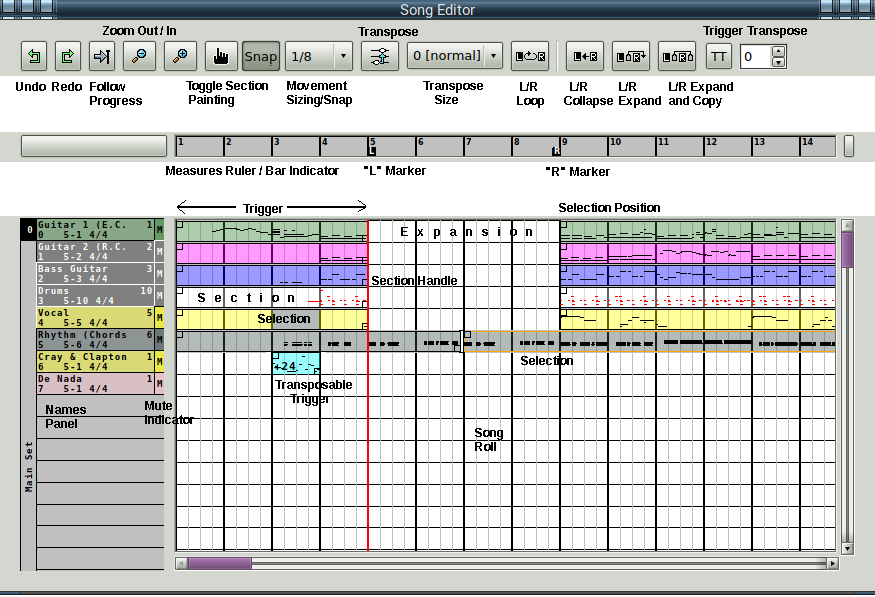
\includegraphics[scale=0.75]{song-editor/song-editor-annotated.png}
   \caption{Song Editor Window, Annotated}
   \label{fig:song_editor_window_annotated}
\end{figure}

   Note the major items shown:

   \begin{enumber}
      \item \textbf{Top Panel}
      \item \textbf{Measures Ruler}
      \item \textbf{Patterns (Names) Panel}
      \item \textbf{Song Roll}
      \item \textbf{Bottom Panel}
   \end{enumber}

   Here are some of the features for the song editor:

   \begin{itemize}
      \item Toggling of the mute state of multiple patterns
         via the name fields of the patterns.
      \item Optional pattern coloring (selected in the Patterns panel)
      \item A configurable progress bar.
      \item \textbf{Undo} and \textbf{Redo} buttons.
      \item A \textbf{Transpose} button and transposition drop-down selector.
      \item Red coloring of events for patterns that are not transposable, such
         as drum tracks.
      \item Horizontal zoom via buttons and keystrokes
   \end{itemize}

   The song editor is not too complex, but for exposition, we break it into
   the sections enumerated above.

\subsection{Song Editor / Top Panel}
\label{subsec:song_editor_top}

   The top panel shown earlier provides quick access to actions
   and configuration.

   \begin{enumber}
      \item \textbf{Undo}
      \item \textbf{Redo}
      \item \textbf{Follow Progress}
      \item \textbf{Zoom Out and Zoom In}
      \item \textbf{Toggle Section Painting}
      \item \textbf{Grid Snap}
      \item \textbf{Transpose}
      \item \textbf{L/R Loop}
      \item \textbf{L/R Collapse}
      \item \textbf{L/R Expand}
      \item \textbf{L/R Expand and Copy}
   \end{enumber}

   \setcounter{ItemCounter}{0}      % Reset the ItemCounter for this list.

   \itempar{Stop}{song editor!stop}
   Stops the playback of the song.
   \index{keys!esc (stop)}
   The keystroke for stopping playback is the \texttt{Escape} character.
   It can be configured to be another character (such as \texttt{Space}, which
   would make the space-bar toggle the playback status).

   \itempar{Play}{song editor!play}
   \index{L marker}
   Starts the playback of the song, starting at the \textbf{L marker}.
   The \textbf{L marker} serves as the start position for playback
   in the song editor.  One can change the start position only when the
   performance is not playing.
   \index{keys!space (play)}
   The default keystroke for starting playback is the \texttt{Space} character.
   \index{keys!esc (stop)}
   The default keystroke for stopping playback is the \texttt{Escape} character.
   \index{keys!period (pause)}
   The default keystroke for pausing playback is the \texttt{Period} character.

   Note that there are no stop, pause, and play buttons in this frame.
   They are supplied by the main window, and the \textbf{Song} tab can be
   activated in the main window.

   \itempar{Undo}{song editor!undo}
   The \textbf{Undo} button rolls back the last change in the layout of a
   pattern.  Each time it is clicked, the most recent change is undone.
%  It is inactive if there is nothing to undo.
   Also implemented via \texttt{Ctrl-Z}.

   \itempar{Redo}{song editor!redo}
   The \textbf{Redo} button reapplies the last change undone by
   the \textbf{Undo} button.
%  It is inactive if there is nothing to redo.
   Also implemented via \texttt{Shift-Ctrl-Z}.

   \itempar{Zoom Out and Zoom In}{song editor!zoom}
   These buttons change the horizontal zoom.
   Zoom can also be changed via the keystrokes \texttt{z}, \texttt{0},
   and \texttt{Z}.

   \itempar{Follow Progress}{song editor!follow}
   \textbf{Follow Progress} toggles the mode of following progress
   for longer songs.  WHen active, the song roll pages right to keep up with
   the progress bar.

   \itempar{Toggle Section Painting}{song editor!paint}
   \textbf{Toggle Section Painting} toggles the ability
   to drag the mouse along the pattern's timeline to create triggers
   to indicate when the pattern plays.
   Short patterns will be duplicated one or more times as
   the mouse is dragged.
   This mode can alsp be changed via the keystrokes \texttt{p} and
   \texttt{x}.

   \itempar{Grid Snap}{song editor!grid snap}
   Indicates the horizontal grid snap for movement actions and trigger drawing.
   Grid snap determine where the pattern boundaries are drawn.
   Unlike the \textbf{Grid Snap} of the pattern editor, the units
   of the song editor snap value are in fractions of a measure length.
   The following values are supported:
   1, 1/2, 1/4, 1/8, 1/16, and 1/32.
%  , and 1/3, 1/6, 1/12, and 1/24.

   \itempar{Transpose}{song editor!transpose}
   \textbf{Transpose} consists of two controls: one to apply
   transposition, and a drop-down menu to select the direction and amount
   of transposition.
   Transposition ranges from minus one octave to plus one octave.

   \itempar{L/R Loop}{song editor!play loop}
   \index{loop mode}
   Activates loop mode. When play is activated, plays the song and loop
   between the
   \index{L marker}
   \index{R marker}
   \textbf{L marker} and the \textbf{R marker}.
   This button is a state button, and its appearance indicates when it is
   depressed, and thus active.
   If this button is deactivated during playback, then playback
   continues past the \textbf{R marker}.
   Note that these markers can be placed using left
   and right mouse clicks, respectively, in the measures ruler.

   \itempar{L/R Collapse}{song editor!collapse}
   This button collapses the song between the \textbf{L marker} and the
   \textbf{R marker}.
   What this means is that, if there is song material (patterns) before the
   \textbf{L marker} and after the \textbf{R marker},
   and the \textbf{Collapse} button is
   pressed, any song material between the L and R markers is erased, and
   the song material after the \textbf{R marker} is moved leftward to
   the \textbf{L marker}.
   Collapsing occurs in all tracks present in the song editor.

   \itempar{L/R Expand}{song editor!expand}
   This button expands the song between the
   \textbf{L marker} and the \textbf{R marker}.
   It inserts blank space between these markers, moving the song material
   that is after the \textbf{R marker}
   to the right by the duration of the blank space.
   Expansion occurs in all tracks present in the song editor.

   \itempar{L/R Expand and Copy}{song editor!expand and copy}
   This button expands the song between the \textbf{L marker} and the
   \textbf{R marker} much like the \textbf{Expand} button.
   However, it also copies the original data that is present after the
   \textbf{R marker}, and pastes it into the newly-available space between
   the L and R markers.

\subsection{Song Editor / Measures Ruler}
\label{subsec:song_editor_measures_ruler}

   \index{measures ruler}
   The measures ruler ("bar indicator")
   consists of a \textsl{timeline} at the top and the 
   \textbf{L marker} and \textbf{R marker} mentioned above.
   There are some hidden details in the measures panel.

   The \textsl{measures ruler} is the ruled and numbered section at the top
   of the arrangement panel.  It provides a place to put the left and right
   markers.  In the \textsl{Seq24} documentation, it is called the "bar
   indicator".

   \index{measures ruler!left-click}
   Left-click in the measures ruler to move and drop an
   \index{L anchor}
   \index{L marker}
   \textbf{L marker} (\textbf{L anchor}) on the measures ruler.
   \index{measures ruler!right-click}
   Right-click in the measures ruler to drop an
   \index{R anchor}
   \index{R marker}
   \textbf{L marker} (\textbf{R anchor}) on the measures ruler.
   
   These markers denote the time intervale from the left of the 
   \textbf{L} marker to the right of the \textbf{R} marker.
   Once these markers are in place, one can then use
	the \textsl{Collapse} and \textsl{Expand} buttons to modify the
   placement of the pattern events.

   Note that the \textbf{L marker} serves as the start position for playback
   in the song editor.  One can change the start position only when the
   performance is not playing.

   \index{marker!mode}
   \index{marker!movement}
   Another way to move the "L" and "R" markers has been added.
   To select which marker will move, first click the upper half of the time
   strip (otherwise, the "L" will move, prematurely) to give it keyboard focus.
   Then press the lower-case
   \index{keys!l}
   \texttt{l} key or the lower-case
   \index{keys!r}
   \texttt{r} key.
   \textsl{There is no visual feedback that one is in the movement mode.}
   Then press the \texttt{Left-Arrow} or \texttt{Right-Arrow}
   key to move the selected marker.

\subsection{Song Editor / Patterns (Names) Panel}
\label{subsec:song_editor_patterns_panel}

   The patterns panel is at the left of the song roll.
   Here are the items to note in the patterns panel:

   \begin{enumber}
      \item \textbf{Number}.
         The number of the screen set.
      \item \textbf{Title}.
         \index{pattern!title}
         \index{pattern!name}
         The title is the name of the pattern, for easy reference.
      \item \textbf{Channel}.
         \index{pattern!channel}
         The channel number appears (redundantly)
         at the right of the title.
      \item \textbf{Buss-Channel}.
         \index{pattern!buss-channel}
         This pair of numbers shows the MIDI buss number used in the pattern
         and the channel used for the pattern.
      \item \textbf{Beat/Measure}.
         \index{pattern!beat}
         This pair of numbers is the standard time-signature of the pattern.
      \item \textbf{Mute Indicator}.
         \index{song editor!mute indicator}
         The letter M is in a black box if the track/pattern is muted, and a
         white box if it is unmuted.
         Left-clicking on the "M" (or the name of the pattern)
         mutes/unmutes the pattern.
         \index{shift left click}
         If the Shift key is held while left-clicking on the M or the pattern
         name, then
         the mute/unmute state of every other active pattern is toggled.
         This feature is useful for isolating a single track or pattern.
      \item \textbf{Empty Track}.
         Completely empty tracks (no track events or meta events)
         are indicated by a dark-gray filling in the pattern column.
         Tracks that have only meta information, but no playable event, are
         indicated by a yellow filling in the pattern column.
   \end{enumber}

   The patterns column shows a list of all of the patterns that have been
   created in the current song.  Each pattern in this list has a track of
   pattern layouts associated with it in the piano roll section.

   \index{patterns column!left-click}
   \index{patterns column!ctrl-left-click}
   \index{song editor!muting}
   Left-clicking on the pattern name or the "M" toggles the muting
   (arming) status of the track.
   It does the same thing if the \texttt{Ctrl} key is held at the same time.

   \index{pattern!shift-left-click}
   \index{song editor!inverse muting}
   \index{song editor!solo}
   \index{shift-left-click solo}
   Shift-left-clicking on the pattern name or the "M" button toggles the muting
   (arming) status of \textsl{all other tracks} except the track that was
   selected.  This action is useful for quickly listening to a single sequence
   in isoloation.

   \index{patterns column!right-click}
   Right-clicking on the pattern name or the "M" button brings up the same
   pattern editing menu as discussed in
   \sectionref{subsubsec:patterns_pattern_filled}.
   Recall that this context menu has the following entries:
   \textbf{Edit...}, \textbf{Event Edit...}, \textbf{Cut}, \textbf{Copy},
   \textbf{Song}, \textbf{Disable Transpose}, and \textbf{MIDI Bus}.

\subsection{Song Editor / Song Roll}
\label{subsec:song_editor_song_roll}

   Also known as the "arrangement panel".
   The "Piano Roll" section of the arrangement panel is where patterns or
   subsections are inserted, deleted, shrunk, lengthened, or moved.
   Actions can be done via the mouse or keyboard.

\subsubsection{Song Editor / Song Roll / Layout}
\label{subsubsec:song_editor_song_roll_layout}

   Here are features to note in the annotated piano roll area
   shown in \figureref{fig:song_editor_window_full_items}:

   \begin{enumber}
      \item \textbf{Trigger Creation}.
         By click-dragging the mouse in paint mode, a series of triggers can be
         created; they indicate where the track will be unmuted and playing.
         See below for more information about triggers.
      \item \textbf{Selection}.
         Clicking inside a trigger selects it.
         Selection is denoted by an orange rectangle around the trigger
         and a dark grey color in the trigger.
         A pattern subsection can be moved by the mouse and deleted by keystrokes.
      \item \textbf{De-selection}.
         \index{song editor!section deselection}
         Left-clicking or right-clicking in an empty area of the song roll
         will deselect the selection.
      \item \textbf{Selection Movement}.
         \index{song editor!selection movement}
         If one grabs (left-click) inside
         the pattern or pattern subsection, that item can be moved
         horizontally, as long as there is room.
%        One can also highlight a pattern section (making it gray),
%        then click the \texttt{p} key to enter "paint" mode, and move the
%        pattern left or right with the arrow keys.
      \item \textbf{Section Length ("handle")}.
         \index{song editor!handle}
         \index{song editor!section length}
         The small squares in two corners of the patterns are the section
         "handles".
         By grabbing a handle with a left-click, the handle can be moved
         horizontally to either lengthen or shorten the pattern to the nearest
         snap position, if there is room to move in the desired direction.
%     \item \textbf{Selection Position}.
%        A selection position is a marker that divides a pattern into two
%        pieces, called \textsl{pattern subsections}.  This makes it easy to
%        select smaller portions of a pattern for editing or deleting.  It
%        is especially useful for making holes in a pattern.
      \item \textbf{Pattern Subsectioning}.
         \index{song editor!split pattern}
         \index{song editor!middle click}
         \index{pattern subsection}
         A middle-click (or ctrl-left-click)
         inside a pattern inserts a selection position
         marker in it, breaking the pattern into two equal pieces.
         We call each piece a \textsl{pattern subsection}.
         This division can be done over and over.
         There are also options for splitting at the nearest snap point.
      \item \textbf{Expansion}.
         \index{song editor!section expansion}
         Originally, all the long patterns of this sample song were continuous.
         But, by setting the L and R markers, and using the \textbf{Expand}
         button, we opened up some silent space in the song, just to be able
         to show it off.
   \end{enumber}

   The \textsl{Seq24} help files refer to work in the song editor as the
   "Performance Editor" or "Performance Mode".  Adding a pattern in this
   window is a bit like adding a note in the pattern editor.
   One clicks, holds, and drags the mouse to insert a copy or copies of the
   pattern associated with the row in which one is dragging.
   The longer one drags, the more copies of the pattern that are inserted.

   \index{song editor!right-click-hold}
   \index{song editor!draw}
   \index{paint mode}
	Right-click on the arrangement panel (roll) to enter
   paint mode, and hold the button.
   Paint mode does not work while the sequence is playing.
   Another way to turn on painting is to
   make sure that the performance editor piano roll has the
   keyboard focus by left-clicking in it, then press the
   \texttt{p} key to enter the paint mode, and
   \texttt{x} escape it.
   See \sectionref{subsubsec:song_editor_song_roll_keystrokes}.

   \index{zoom}
   \index{song editor!zoom}
   The song editor supports horizontal zoom in the piano roll.
   This feature is accessible via the buttons, and also
   accessible via keystrokes.
   The zoom feature also modifies the time-line.

   \index{song editor!left-click-right-hold}
   \index{song editor!insert}
   A left-click with a simultaneous right-click-hold inserts one copy of the
   pattern.  The inserted pattern shows up as a box with a tiny
   representation of the notes visible inside.  Some patterns can
   be less than a measure in length, resulting in a tiny box.
   \index{song editor!right-left-hold-drag}
   \index{song editor!multiple insert}
   To keep adding more copies of the pattern, continue to hold both buttons
   and drag the mouse rightward.

   \index{song editor!middle-click}
   Middle-click i(or ctrl-left-click) on a trigger in a pattern row
   to splits the trigger into two triggers.
   \index{pattern!split}
   \index{song editor!pattern subsection}
   This splits the pattern into two equal \textsl{pattern subsections}.
   Each middle-click on the pattern adds a new selection position,
   halving the size of the subsections as more pattern subsections are
   added.  The \texttt{allow\_snap\_split} option in the 'rc' file
   allows the split to be made at the nearest snap point instead of in the middle.

   \index{song editor!left-click}
   \index{song editor!selection}
   When a pattern or a pattern subsection is left-clicked in the piano
   roll, it is marked with a dark gray filling.
   It can then be moved horizontally if there is room, or be deleted or copied for
   later pasting.

   \index{song editor!right left click}
   \index{song editor!deletion}
   When a right-left-click action is done in this gray area, the result
   is to \textsl{delete} that pattern section or subsection.
   \index{keys!delete}
   One can also hit the \texttt{Delete} key.

\subsubsection{Song Editor / Song Roll / Keystrokes}
\label{subsubsec:song_editor_song_roll_keystrokes}

   There are a number of useful keystrokes in the song roll that can be used once
   is has focus, by clicking in it.

   \begin{itemize}
      \item Enter "paint" mode.
         The \texttt{p} key enters paint mode, where additional triggers
         can be added by click-dragging on a pattern row.
         The \texttt{x} key leaves this mode.
         The "finger" button and the mouse cursor both indicate the status.
      \item Start/Pause button functionality.
         When the song roll has keyboard focus,
         the \texttt{Space} key starts and stops playback, rewinding to the
         beginning when stopped.
         The \texttt{.} (period) key starts and pauses playback, without
         rewinding.
         This functionality is similar to that of the main window, but
         these keys are not reconfigurable in the song roll.
      \item Undo/Redo/Cut/Copy/Paste of a selected section.
         Provided by buttons and by these keystrokes:
         \texttt{Ctrl-Z}. Undo.
         \texttt{Shift-Ctrl-Z}. Redo.
         \texttt{Ctrl-X}. Cut.  Removes the selection.
            \index{keys!backspace}
            \index{keys!delete}
            \index{keys!ctrl-x}
            Can also be done with the \texttt{Delete} and
            \texttt{Backspace} keys.
            The deletion can be undone.
         \texttt{Ctrl-C}. Copy.
         \index{keys!ctrl-c}
         \index{keys!copy}
         Copies the trigger for later usage.
         \texttt{Ctrl-V}. Paste.
            \index{keys!ctrl-v}
            \index{keys!paste}
            Puts the roll into paste mode.
            When inserted, each insert goes immediately
            after the current item or the previous insertion.  The same can be
            done for whole patterns.
      \item Horizontal (Time) Zoom.
         Provided by buttons and by these keystrokes:
         \texttt{Z}. Zoom in.
         \texttt{z}. Zoom out.
         \texttt{0}. Reset zoom.
      \item Paging.  Paging by keystroke is not yet complete.
      Here is what can be done.
      One can page up and down vertically in the arrangement
      panel using the
      \index{keys!page-up}
      \texttt{Page Up} and 
      \index{keys!page-down}
      \texttt{Page Down} keys.
%     One can go to the top using the 
%     \index{keys!home} Home key,
%     to the bottom using the
%     \index{keys!end} End key.
      One can page left and right horizontally in the arrangement
      panel using the
      \index{keys!up-arrow} \texttt{Up-Arrow} and 
      \index{keys!down-arrow} \texttt{Down-Arrow} keys.
%     \index{keys!shift-page-up} Shift Page Up and 
%     \index{keys!shift-page-down} Shift Page Down keys.
%     One can go to the leftmost position using the 
%     \index{keys!shift-home} Home key,
%     and to the rightmost position using the
%     \index{keys!shift-end} End key,
   \end{itemize}

\subsection{Song Editor / Bottom Panel}
\label{subsec:song_editor_bottom}

   The bottom panel is simple, consisting of a stock horizontal scroll bar.

\begin{comment}

   and a small button, called the \textbf{Grow} button, labelled with a
   "\textbf{$>$}".

   \index{grow button}
   \index{song editor!grow}
   The \textbf{Grow} button adds to the number of measures that exist
   in the song editor. The visual effect is very subtle, resulting only
   in a small change in the thumb of the horizontal scroll-bar, unless one
   is at the right end of the piano roll.  Then, one can see the added
   measures.  Usually about 128 at a time are added, but this depends on the
   value of PPQN in force.

\end{comment}

%-------------------------------------------------------------------------------
% vim: ts=3 sw=3 et ft=tex
%-------------------------------------------------------------------------------


% Event Editor

%-------------------------------------------------------------------------------
% event_editor
%-------------------------------------------------------------------------------
%
% \file        event_editor.tex
% \library     Documents
% \author      Chris Ahlstrom
% \date        2016-01-02
% \update      2021-01-28
% \version     $Revision$
% \license     $XPC_GPL_LICENSE$
%
%-------------------------------------------------------------------------------

\section{Event Editor}
\label{sec:event_editor}

   The \textsl{Seq66} \textbf{Event Editor} is used to view and edit,
   in detail, the events present in a loop / sequence / pattern / track.
   It is accessed by right-clicking on a pattern in the \textbf{Live} frame,
   then selecting the \textbf{Edit pattern in tab} menu entry.

   The event editor is not very sophisticated.
   It is a basic editor for simple edits, viewing, and trouble-shooting.
   Viewing and scrolling generally work;
   editing, deleting, and inserting events work.
   But there are many possible interactions between event links
   (Note Off events linked to Note On events),
   performance triggers, and the pattern,
   performance, and event editor dialogs.
   Surely some bugs still lurk.
   If anything bad happens, do \textsl{not} press the
   \textbf{Save to Sequence} button!
   If the application aborts, let us know!

   Here are the major "issues":

   \begin{enumerate}
      \item It requires the user to know the details
         about MIDI events and data values.
      \item It does not present handy dropdown lists for various items.
      \item It does not detect any changes made to the sequence in the
         pattern editor, and so both editors cannot be brought on screen at the
         same time for the same pattern.
      \item It does not have an undo function.
      \item It cannot mark more than one event for deletion or modification.
      \item There is no support for dragging and dropping of events.
   \end{enumerate}

%  If, some day, we find ourselves needing
%  that kind of functionality, then we can add it.
%  There may also be issues with interactions between the event editor and
%  things like the performance editor and triggers.

   The event editor is a good way to see the events in a sequence,
   and to delete or modify problematic events.
   Additionally, it can be used to add \textbf{Set Tempo} meta events.
   \index{sequence extension}
   \index{pattern extension}
   If an event is added that has a time-stamp beyond the current
   length of the sequence, then the length of the sequence is extended.
   Unlike the event pane in the pattern editor, the event-editor
   dialog shows all types of events at once.

\begin{figure}[H]
   \centering
   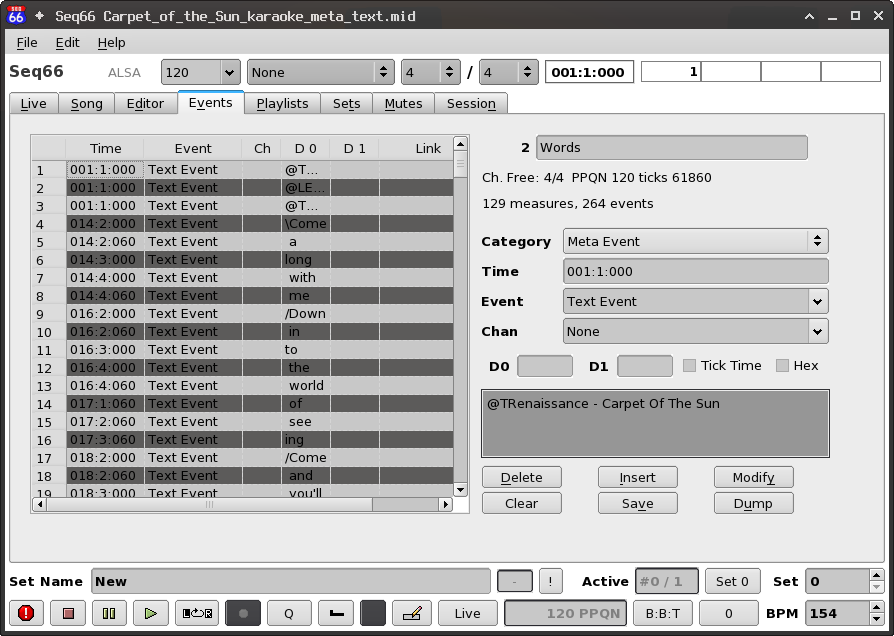
\includegraphics[scale=0.85]{event-editor/event-editor-tab.png}
   \caption{Event Editor Window}
   \label{fig:event_editor_window}
\end{figure}

   The event-editor dialog is fairly complex.
   For exposition, we break it down into a few sections:

   \begin{enumber}
      \item \textbf{Event Frame}
      \item \textbf{Info Panel}
      \item \textbf{Edit Fields}
      \item \textbf{Bottom Buttons}
   \end{enumber}

   The event frame is a list of events, which can be traversed, and edited.
   The fields in the right panel show the name of
   the pattern containing the events and other information about the
   pattern.  The edit fields provide text fields for viewing and entering
   information about the current event, and buttons to delete, insert, and
   modify events.  The bottom buttons allow changes to be saved and the editor
   to be closed.  
   The following sections described these items in detail.

\subsection{Event Editor / Event Frame}
\label{subsec:event_editor_frame}

   The event frame is the event-list shown on the left side of the
   event editor.  It is accompanied by a vertical scroll-bar, for moving one
   line or one page at a time.
   Mouse or touchpad scrolling can be used to move up and down
   in the event list.  This movement is even easier than reaching for the
   scrollbars.

\subsubsection{Event Frame / Data Items}
\label{subsec:event_frame_data}

   The event frame shows a list of numbered events, one per line.
   The currently-selected event is highlighted in cyan text on a black
   background.  Here is an example of the data line for a MIDI event:

   \begin{verbatim}
      17-003:3:128 Note On   Chan 3    Key 66 Vel 107
   \end{verbatim}

   This line consists of the following parts:

   \begin{enumber}
      \item \textbf{Index Number}
      \item \textbf{Time Stamp}
      \item \textbf{Event Name}
      \item \textbf{Channel Number}
      \item \textbf{Data Bytes}
   \end{enumber}

   \setcounter{ItemCounter}{0}      % Reset the ItemCounter for this list.

   \itempar{Index Number}{event editor!index number}
   Displays the index number of the event.
   This number is purely for reference, and is not part
   of the event.  Events in the pattern are numbered from 0 to the number of
   events in the pattern.

   \itempar{Time Stamp}{event editor!time stamp}
   Displays the time stamp of the event,
   which indicates the cumulative time of the event in the pattern.
   It is displayed in the format of "measure:beat:divisions".
   The measure values start from 1, and range up to the number of measures in
   the pattern.
   The beat values start from 1, and range up to the number of beats in the
   measure.
   The division values range from 0 up to one less than the
   \index{ppqn}
   PPQN (pulses per quarter note) value for the whole song.
   \index{ppqn!\$ shortcut}
   As a shortcut, one can use the dollar sign ("\$") to represent
   PPQN-1.

   \itempar{Event Name}{event editor!event name}
   Displays the name of the event.
   The event name indicates what kind of MIDI event it is. 
   The following event names are supported:

   \begin{enumber}
      \item \textbf{Note Off}
      \item \textbf{Note On}
      \item \textbf{Aftertouch}
      \item \textbf{Control Change}
      \item \textbf{Program Change}
      \item \textbf{Channel Pressure}
      \item \textbf{Pitch Wheel}
      \item \textbf{Tempo}
   \end{enumber}

%  \textbf{Note that these are all MIDI \textsl{channel events}.
%  Support for MIDI \textsl{system events} is in place, but is not
%  ready for exposure to the user.}

   \itempar{Channel Number}{event editor!channel number}
   Shows the channel number (for channel-events only) re 0, not 1.
   For the user, of course, MIDI channels always range from
   1 to 16.  Internally, they range from 0 to 15.

   \itempar{Data Bytes}{event editor!data bytes}
   Shows the one or two data bytes for the event.

   Note Off, Note On, and Aftertouch events requires a byte for the key (0 to
   127) and a byte for the velocity (also 0 to 127).
   Control Change events require a control code and a value for that control
   code.  Pitch wheel events require two bytes to encode the full range of
   pitch changes.
   Program change events require only a byte value to pick the patch or program
   (instrument) to be used for the sequence.  The Channel Pressure event
   requires only a one-byte value.
   Tempo requires a number (e.g. "120.3") to be typed in.

\subsubsection{Event Frame / Navigation}
\label{subsec:event_frame_navigation}

   Moving about in the event frame is straightforward, but has some
   wrinkles to note.
   Navigation with the mouse is done by moving to the desired event and
   clicking on it.  The event becomes highlighted, and its data items are shown
   in the "info panel".
   There is no support for dragging and dropping events in the event frame.

   The scrollbar can be used to move within the frame, either by one line at a
   time, or by a page at a time.  A page is defined as one frame's worth of
   lines, minus 5 lines, for some overlap in paging.

   Navigation with keystrokes is also supported, for the Up and Down arrows and
   the Page-Up and Page-Down keys.  Note that using the Up and Down arrows by
   holding them down for awhile causes autorepeat to kick in, and the updates
   become very erratic and annoying.  Use the scrollbar or page keys to
   move through multiple pages.  Home and End also work.

\subsection{Event Editor / Info Panel}
\label{subsec:event_editor_info}

   The "info panel" is simply a read-only list of properties on the top right
   of the event editor.  It serves to remind the used of the pattern being
   edited and some characteristics of the pattern and the whole song.
   Five items are shown:

   \begin{enumber}
      \item \textbf{Sequence Number and Name}.
         A bit redundant, as the window caption for the event editor
         also shows the pattern name.
         It can be set in the pattern editor.
      \item \textbf{Time Signature}.
         A pattern property, shown only as a reminder.
         It can be set in the pattern editor.
      \item \textbf{PPQN}
         Shows the "parts per quarter note", or resolution of the
         whole song.  The default PPQN of \textsl{Seq66} is 192.
      \item \textbf{Sequence Channel}
         In \textsl{Seq66}, the channel number is a property of the
         pattern.  All channel events in the pattern get routed to the same
         channel, even if somehow the event itself specifies a different
         channel.
      \item \textbf{Sequence Count}
         Displays the current number of events in the pattern.
         This number changes as events are inserted or deleted.
   \end{enumber}

\subsection{Event Editor / Edit Fields}
\label{subsec:event_editor_fields}

   The edit fields show the values of the currently-selected event.  They allow
   changing an event, adding a new event, or deleting the currently-selected
   event.

   \begin{enumber}
      \item \textbf{Event Category} (read-only)
      \item \textbf{Event Timestamp}
      \item \textbf{Event Name}
      \item \textbf{Data Byte 1}
      \item \textbf{Data Byte 2}
      \item \textbf{Delete Current Event}
      \item \textbf{Insert New Event}
      \item \textbf{Modify Current Event}
   \end{enumber}

   \textbf{Important}: changes made in the event editor
   are \textsl{not} written to the sequence until the \textbf{Save to Sequence}
   button is clicked.  If one messes up an edit field, just click on the event
   again; all the fields will be filled in again.
   That's as much "undo" as the event-editor offers at this time, other than
   closing without saving.

   \setcounter{ItemCounter}{0}      % Reset the ItemCounter for this list.

   \itempar{Event Category}{event editor!event category}
   Displays the event category of the event.  Currently, only channel events
   can be handled, but someday we hope to handle the wide array of system
   events, and perhap even system-exclusive events.

   \itempar{Event Timestamp}{event editor!event timestamp}
   Displays the timestamp of the event.  Currently only the
   "measure:beat:division" format is fully supported.
   We allow editing (but not display) of the timestamp in
   pulse (divisions) format and "hour:minute:second.fraction" format, but
   there are bugs to work out.

   If one wants to delete or modify an event, this field does not need to be
   modified.  If this field is modified, and the \textbf{Modify Current Event}
   button is pressed, then the event will be moved.  This field can locate
   a new event at a specific time.  If the time is not in the current frame,
   the frame will move to the location of the new event and make it the current
   event.

   \itempar{Event Name}{event editor!event name}
   Displays the name of the event, and allows entry of an event name.
   The event name indicates what kind of MIDI event it is. 
   The following event names are supported:

   \begin{enumber}
      \item \textbf{Note Off}
      \item \textbf{Note On}
      \item \textbf{Aftertouch}
      \item \textbf{Control Change}
      \item \textbf{Program Change}
      \item \textbf{Channel Pressure}
      \item \textbf{Pitch Wheel}
      \item \textbf{Tempo}
   \end{enumber}

   Typing in one of these names changes the kind of event if the event is
   modified.  Abbreviations and case-insensitivity can be used to reduce the
   effort of typing.
   This handling of the editing of the event name is still a bit clumsy.
   It would be better to provide a drop-down list for more painless
   selection of events.  Some day.

   \itempar{Data Byte 1}{event editor!data byte 1}
   Allows modification of the first data byte of the event.
   One must know what one is doing.
   The scanning of the digits is very simple:  start with the first digit, and
   convert until a non-digit is encountered.  The data-byte value can be
   entered in decimal notation, or, if prepended with "0x", in hexadecimal
   notation.

   \itempar{Data Byte 2}{event editor!data byte 2}
   Allows modification of the second data byte of the event (if applicable
   to the event).
   One must know what one is doing.
   The scanning of the digits is as noted above.

   \itempar{Delete Current Event}{event editor!delete event}
   Causes the selected event to be deleted.
   The frame display is updated to move following events upward.

   \index{bugs!event delete key}
   \index{bugs!event insert key}
   \textsl{Seq66} would support using the Delete and Insert keys to
   supplement the buttons, but the Delete key is needed for editing the event
   data fields.
   The current structure of the dialog prevents using it for both
   the frame and the edit fields.  Therefore, \textsl{Seq66} allows the
   usage of the \textbf{asterisk} keys (regular and keypad) for
   deletion.

   \itempar{Insert New Event}{event editor!insert event}
   Inserts a new event, described by the 
   \textbf{Event Timestamp},
   \textbf{Event Name},
   \textbf{Data Byte 1}, and
   \textbf{Data Byte 2} fields.
   The new event is placed in the appropriate location for the given timestamp.
   If the timestamp is at a time that is not visible in the frame, the frame
   moves to show the new event, so be careful.

   \itempar{Modify Current Event}{event editor!modify event}
   Deletes the current event, and inserts the modified event,
   which is placed in the appropriate location for the given
   timestamp.

\subsection{Event Editor / Bottom Buttons}
\label{subsec:event_editor_buttons}

   The buttons at the bottom of the event editor round out the functionality of
   this dialog.

   \begin{enumber}
      \item \textbf{Save to Sequence}
      \item \textbf{Close}
   \end{enumber}

   \setcounter{ItemCounter}{0}      % Reset the ItemCounter for this list.

   \itempar{Save to sequence}{event editor!save to sequence}
   Saves the event container back to the sequence from
   whence the events came.  This button does not close the dialog; further
   editing can be performed.  The Save button is enabled only if
   some unsaved changes to the events exist.
%  Note that there may still be some subtle bugs in the dialog editor, so be
%  careful about pressing this button.

   Any sequence/pattern editor that is open should be reflected
   in the pattern editor once this button is pressed.  However, at present,
   simultaneous use of the pattern editor and event editor has been disabled.
   \index{bugs!event delete segfault}
   If both the event editor and the pattern editor are open for a sequence
   (currently disabled), and
   some events are deleted in the event editor, and the
   \textbf{Save to Sequence} button is pressed, the pattern editor would
   crash and
   takes down \textsl{Seq66} with it.  Therefore, when either editor is
   open for a given sequence, the right-click menu entries that bring them up
   are hidden.

   \itempar{Close}{event editor!close}
   Closes the event editor.
   Any unsaved event changes are discarded.
   There is a "modification indicator" to show that the events have
   been modified.

   Again, good luck with the dialog.  Bug reports are appreciated.

%-------------------------------------------------------------------------------
% vim: ts=3 sw=3 et ft=tex
%-------------------------------------------------------------------------------


% Session Management

%-------------------------------------------------------------------------------
% seq66 sessions
%-------------------------------------------------------------------------------
%
% \file        sessions.tex
% \library     Documents
% \author      Chris Ahlstrom
% \date        2020-10-03
% \update      2023-11-05
% \version     $Revision$
% \license     $XPC_GPL_LICENSE$
%
%  Provides a discussion of how Seq66 supports session management, specifically
%  the Non Session Manager.
%
%-------------------------------------------------------------------------------

\section{Session Management}
\label{sec:sessions}

   A session is a group of applications and their configuration and
   connections.
   Session management recreate complex setups and provides some uniformity
   of application control in a session.
   The first thing to do for session management is to make sure that the
   application is capable of various levels of session management, from
   \textsl{UNIX} signals to
   a complete session manager like the \textsl{Non/New Session Manager}.
   Basic session management consist of being able to properly start the
   application and let it run properly during its life-cyle, whether it is a
   command-line application or a graphical application.
   \textsl{Seq66} supports session management in three ways:

   \begin{enumber}
      \item \textbf{Signals}.
         During a normal run, \textsl{Seq66} will respond
         to signals to save and to quit.
         The normal configuration files and command-line options will be
         used, and can be marked to be saved at exit.
         This mode is useful with \textsl{nsm-proxy}, a way to script
         applications that don't have \textsl{NSM} support.
      \item \textbf{JACK Session}
         Deprecated, but implemented nonetheless.
         Many still use it.
         This session manager allows the configuration files to be stored in
         a separate directory, for \textsl{Seq66} to be started, and files to
         be saved.  No restrictions on where the MIDI files can be stored.
      \item \textbf{Non Session Manager}
         Known as \textsl{NSM}, and in the form of a fork of that project,
         \textsl{New Session Manager},
         it provides a replacement for \textsl{JACK Session}.
         It requires all files to be
         stored in a session directory, and provides commands for saving,
         quitting, hiding/showing the user-interface, and more.
         Like \textsl{JACK Session}, it allows control over the startup of
         multiple applications, the process of saving a session, and provides a
         way to save their patching (connections) in \textsl{JACK}.
         However, it supports more functionality and has
         strict requirements the application must follow.
         Development of NSM has, for various reasons, been suspended, but
         offshoots such as \textsl{Agordejo} (\cite{agordejo})
         and \textsl{RaySession} (\cite{raysession}), which are front ends for
         the \textsl{New/Non Session Manager} (\cite{nsm}),
         continue to advance.
   \end{enumber}

   For session management, \textsl{NSM} is the way to go.
   \textsl{JACK} session management is provided for those who still use it.
   There are other session solutions, such as \textsl{aj-snapshot},
   \textsl{Claudia}, and \textsl{Chino}.
   For now, we do not discuss them.

   The desired session can be set in the \textbf{Edit / Preferences /
   Session} tab.  But note that, if started by \textsl{NSM}, \textsl{Seq66}
   will detect it and nonetheless set up for NSM usage.
   The \textsl{NSM} setting is
   useful for attaching to a pre-existing known session.
   \textsl{JACK} session management events are processed
   only if \textsl{JACK} is selected.
   \textsl{JACK} session management will still start \textsl{Seq66} in
   an existing session, if \textsl{JACK} is
   not selected.

   Also note that sometimes one will want the session manager to make the JACK
   connections.  In this case, go to
   \textbf{Edit / Preferences / JACK / Jack Auto-Connect}, uncheck that option,
   and restart \textsl{Seq66}.
   This option, \texttt{jack-auto-connect}
   can also be changed in the 'rc' file.
   The \textsl{NSM} tool called \textsl{jackpatch} can also be used to manage
   connections.

\subsection{Session Management / Signals}
\label{subsec:sessions_signals}

   \index{sessions!signals}
   By default, the basic form of session management in
   \textsl{Seq66} occurs by signals.  A
   session manager can start \textsl{Seq66}, and it can tell \textsl{Seq66} to
   save or stop.  Starting is done by a system call to spawn the application.
   The save and stop actions are supported by sending the following signals to
   the application:

   \begin{itemize}
      \item \texttt{SIGINT}.
         This signal stops \textsl{Seq66}. It corresponds
         to using \texttt{Ctrl-C} from the command-line to stop \textsl{Seq66}.
         This signal should work for both the graphical and command-line
         application.  As \textsl{Seq66} shuts down, it does its normal saving
         of the current state of the configuration.
      \item \texttt{SIGTERM}.
         This signal also stops \textsl{Seq66}.  It can
         be sent by an application to exit \textsl{Seq66}.
      \item \texttt{SIGUSR1}.
         This signal tells \textsl{Seq66} to save.  This
         action will save the current MIDI file.
   \end{itemize}

   One application that can control \textsl{Seq66} via these signals, when not
   in session mode, is \textsl{nsm-proxy}:

      \url{https://non.tuxfamily.org/wiki/nsm-proxy}

   \textsl{NSM-Proxy} is a simple \textsl{NSM} client for wrapping non-NSM
   capable programs. It enables the use of programs supporting LADISH Level 0
   and 1, and programs which accept their configuration via command-line
   arguments.  There is a command-line version and a graphical version.
   More to come on how to use \texttt{nsm-proxy}.

\subsection{Session Management / JACK Session}
\label{subsec:sessions_jack}

   Although deprecated by the \textsl{JACK} authors in favor of \textsl{NSM},
   we are implementing \textsl{JACK} session (JS) management for the benefit of
   people who either do not know of \textsl{NSM} or do not want to implement or
   use it.

   \textsl{Seq66}, as a JS-aware applications, is set up to

   \begin{enumerate}
      \item Register with a JS manager.
      \item Respond to messages from the JS manager.
      \item Be startable with session information.
   \end{enumerate}

   A response to a JS message will do one of the following:

   \begin{itemize}
      \item Save the application's state into a file, where the directory is
         supplied by the session manager.
      \item Reply to the session manager with a command-line that starts the
         application, with information to restore its state, such as
         the name of the file holding its state information.
   \end{itemize}

	JS-aware clients identify themselves to the session manager by a UUID
	(unique universal identifier). The session manager provides it to
	the client application as an integer represented as a string.
   This can be passed to the session manager when registering, but
   \textsl{Seq66} just uses the value given to it (for now).

%  but should also be passed back to the client when it is restarted
%by the session manager. This is done by a command line argument to the
%application, and the format of the command line is also up to the client.

   For this discussion, we will use the \textsl{JACK} session implementation in
   the \textsl{QjackCtl} application.
   Also, read the script stored in
   \texttt{seq66/data/linux/startqjack} to set up
   \textsl{QjackCtl} to run \textsl{JACK} and kick off
   \textsl{a2jmidid}; it should be added to the \textsl{QjackCtl}
   configuration.

   Once that setup is made (installing the script and configuring
   \texttt{qjackctl}, then start \texttt{qjackctl}.
   Verify that there are a number of system audio and MIDI playback and capture
   port, \textsl{PulseAudio JACK} sinks and sources if the system uses
   \textsl{PulseAudio}, and that there are "a2j" MIDI ports for all of your USB
   hardware devices.

   Then start \textsl{Qsynth} so it uses \textsl{jack} for MIDI and
   \textsl{jack} (or \textsl{pulseaudio}) for audio.
   Then run \textsl{Seq66} with \textsl{JACK} for slave transport and for MIDI
   (either command works the same):

   \begin{verbatim}
      $ qseq66 --jack-slave --jack-midi
      $ qseq66 --jack-slave --jack
   \end{verbatim}

   Load a file, make sure its MIDI output goes to "fluidsynth" or "qsynth", and
   plays.
   In your desired location (e.g. \texttt{~/.config/seq66/sessions},
   create a new session directory (e.g. \texttt{qtest}).

   In \textsl{qjackctl}, open the \textbf{Sessions} dialog.
   Click \textbf{Save}, and choose the directory just created.
   In the dialog should appear entries for MIDI capture and playback for
   "fluidsynth" and "seq66", all the "a2j" USB devices,
   plus an entry for \textsl{JACK} client
   \textsl{seq66master} or \textsl{seq66slave} that shows
   something like:

   \begin{verbatim}
qseq66 --jack --jack-master --jack-session-uuid 84670 --home ${SESSION_DIR}
qseq66 --jack --jack-slave --jack-session-uuid 84670 --home ${SESSION_DIR}
   \end{verbatim}

   In the \textbf{Connections} dialog of \textsl{QjackCtl}, all of these ports
   will be shown in the MIDI tab, auto-connected appropriately.
   In the sessions directory that was created, will be seen an
   empty \texttt{seq66master}
   or \texttt{seq66slave} directory, and a
   \texttt{sessions.xml} configuration file containing the information shown in
   the sessions dialog.
   Exit \textsl{Seq66}, \textsl{QSynth} and \textsl{QjackCtl}
   (in that order).

   One issue is that \textsl{QSynth}
   does not support \textsl{JACK Session}.
   Try it with \textsl{Yoshimi}, which does support it.

\subsection{Seq66 Session Management / NSM}
\label{subsec:sessions_nsm}

   \index{sessions!nsm}
   The \textsl{Non Session Manager} is an API implementation for session
   management for Linux audio/MIDI.
   \textsl{NSM} clients use a well-defined
   \index{sessions!OSC}
   \textsl{OSC} protocol (\cite{osc})
   to communicate with the session management daemon.

   Note that \textsl{Non Session Manager} is in a state of suspended
   development, and has been reimplemented as a \textsl{GitHub} project,
   the \textsl{New Session Manager}.

   The applications it manages should be installed normally (that is,
   for system-wide usage, in
   \texttt{/usr/bin/} or \texttt{/usr/local/bin}).

\subsubsection{Session Management / NSM / First Run Without NSM}
\label{subsec:sessions_nsm_first_run_without_nsm}

   This section discusses what happens when \textsl{Seq66} is installed, then
   run outside of any session from the console or an application menu.
   For a discussion where \textsl{Seq66} is run for the first time under
   \textsl{NSM},
   see \sectionref{subsec:sessions_nsm_first_run_in_nsm}.

   Generally, after installing \textsl{Seq66}, or when creating a new setup
   (such as a play-list) it is good to run it normally first, to simplify
   trouble-shooting.
   This action creates the configuration files in the default location,
   \texttt{/home/user/.config/seq66}:

\begin{verbatim}
   $ qseq66 
   No 'rc' file, will create: qseq66.rc/ctrl/midi/mutes
   No 'usr' file, will create: /home/user/.config/seq66/qseq66.usr
   File exists: /home/user/.config/seq66/qseq66.rc
   Saving initial config files to session directory!
   Writing 'rc': /home/user/.config/seq66/qseq66.rc
   Writing 'ctrl': /home/user/.config/seq66/qseq66.ctrl
   Writing 'mutes': /home/user/.config/seq66/qseq66.mutes
   Writing 'usr': /home/user/.config/seq66/qseq66.usr
   . . .
\end{verbatim}

   Then exit \textsl{Seq66} to ensure the configuration files are created.
   Optionally, in this initial setup,
   one can also create a 'playlist' file and a 'drums' file, or
   copy them from:

   \begin{verbatim}
      /usr/share/seq66-0.91/data/samples
   \end{verbatim}

   to

   \begin{verbatim}
      /home/user/.config/seq66
   \end{verbatim}

   and modify them appropriately.
   Another first-time modification to consider is setting up \textsl{Seq66} to
   use the \textsl{JACK} audio/MIDI subsystem (on \textsl{Linux}).
   In the 'rc' file, look for the following line:

   \begin{verbatim}
      [jack-transport]
      jack-midi = false
   \end{verbatim}

   And change it to:

   \begin{verbatim}
      [jack-transport]
      jack-midi = true
   \end{verbatim}

   Another first-time modification to consider is using virtual ports (option
   \texttt{--manual-ports}) versus the automatic port connections
   \textsl{Seq66} normally makes.
   This setup allows the user to manually make connections between
   \textsl{Seq66} and other MIDI applications.
   In the 'rc' file, look for the following lines:

\begin{verbatim}
   [manual-ports]
   virtual-ports = false   # 'true' = manual (virtual) ALSA or JACK ports
   output-port-count = 8   # number of manual/virtual output ports
   input-port-count = 4    # number of manual/virtual input ports
\end{verbatim}

   And change the virtual-ports line to:

\begin{verbatim}
   [manual-ports]
   virtual-ports = true    # 'true' = manual (virtual) ALSA or JACK ports
\end{verbatim}

   It is then important to start \texttt{qseq66} in the normal manner again,
   and verify that everything works as expected.

   We have added a command, \textbf{File / Import / Import Project}
   command to import the configuration files from one directory into the
   current \textsl{NSM} session configuration directory.
   This import used to be automatic, but is too surprising to an unsuspecting
   user.

\subsubsection{Seq66 Session Management / NSM / Run in NSM}
\label{subsec:sessions_nsm_first_run_in_nsm}

   Note: When \textsl{Seq66} is run in \textsl{NSM} for the first time,
   a stock default configuration is saved when
   \textsl{Seq66} exits.
   This is different from earlier behavior, where the home configuration was
   imported automatically.
   Now, the user must use the
   \textbf{File / Import / Import Project...}
   command.

   For illustration, we run \textsl{NSM} from a terminal window, which can be
   very helpful when problems occur.

\begin{verbatim}
   $ non-session-manager
   [non-session-manager] Starting daemon...
   [nsmd] Session root is: /home/user/NSM Sessions
   NSM_URL=osc.udp://mycomputer.mls:19625/
   [nsmd] Listing sessions
\end{verbatim}

   \index{sessions!non-starter}
   \index{sessions!liblo library}
   If \textsl{NSM} refuses to start, make sure that the \texttt{liblo} library
   from the OSC project is installed.
   \index{sessions!/etc/hosts}
   \index{sessions!loopback interface}
   If it is installed, then check the
   \texttt{/etc/hosts} file to make sure that a loopback interface is
   defined. In some versions of \textsl{Linux}, it isn't defined properly,
   and the \textsl{NSM} daemon (\texttt{nsmd}) will not start.
   Here is an example of the loopback installed in \textsl{Debian Sid};

\begin{verbatim}
   127.0.0.1   localhost
   127.0.1.1   mycomputer.mls mycomputer
\end{verbatim}

   The NSM user-interface (not shown here) that comes up is empty at first.
   So create a session by clicking the \textsl{NSM}
   \textsl{New} button, and entering a session name
   (here, "\textbf{Seq66}") in the
   prompt that comes up.  In the console window, a couple of 
   \texttt{/nsm/server/new} \textsl{OSC} messages
   about the creation of the session appear.

\begin{verbatim}
   [non-session-manager] Sending new for: Seq66
   [nsmd] Creating new session "Seq66"
   [non-session-manager] /nsm/server/new says Created.
   [non-session-manager] /nsm/server/new says Session created
\end{verbatim}

   Next, click the \textsl{Add Client to Session}, and, since
   \texttt{qseq66} has been installed system-wide, it is in the \texttt{PATH}
   and its executable name can be entered simply: "\texttt{qseq66}".
   A number of console messages from
   \textsl{Seq66} appear, plus some messages from \textsl{NSM}.

\begin{verbatim}
   [non-session-manager] Sending add for: qseq66
   [nsmd] Process has pid: 2797436
   [nsmd] Launching qseq66
   [nsmd] Got announce from seq66
   [nsmd] Client was expected.
   [nsmd] Process has pid: 2797436
   [nsmd] The client "seq66" at "osc.udp://127.0.0.1:13318/" informs us it's
    ready to receive commands.
\end{verbatim}

   Important: the \textsl{Seq66} user-interface will not show at first.
   It is hidden so that the screen is not inundated with the windows of all the
   applications that are (eventually) running under the session.
   This is especially annoying with tiled window managers.
   In order to see the \textsl{Seq77} user-interface, click on
   the \textbf{GUI} button in the session line shown in the \textsl{NSM} window .

   Once \textsl{Seq66} is running under \textsl{NSM},
   then click the \textbf{Save}
   button at the top of the \textsl{NSM} interface in order
   to save the session information.
   This is an \textsl{important} step.
   After \textsl{Seq66} exits,
   one can see what has been created to support the session;
   the directory that \textsl{NSM}
   creates by default is \texttt{/home/user/NSM Sessions}.
   \index{nsm!old session}

\begin{verbatim}
   $ pwd
   /home/user/NSM Sessions
   $ lstree Seq66
   Seq66/
     +-- seq66.nGJDW/
     |   +-- config/
     |   |   +-- qseq66.ctrl
     |   |   +-- qseq66.drums
     |   |   +-- qseq66.mutes
     |   |   +-- qseq66.palette
     |   |   +-- qseq66.playlist
     |   |   +-- qseq66.rc
     |   |   +-- qseq66.usr
     |   +-- midi/
     +-- session.nsm
\end{verbatim}

   \textbf{Important}: If one is running a recent "New" version of the 
   \textsl{Non Session Manager}, then the session data is not stored
   in \texttt{/home/user/NSM Sessions},
   but in
   in \texttt{/home/user/.local/share/nsm},
   Thus the above would be located differently:
   \index{nsm!new session}

\begin{verbatim}
   $ cd ~/.local/share/nsm    # the value of $XDG_DATA_HOME
   Seq66/
     +-- seq66.nGJDW/
     [ the rest is the same as above ]
\end{verbatim}

   So \textsl{NSM} has created a directory with the session name we gave it:
   \texttt{Seq66}.

   \textsl{Side note: the \texttt{nsmd} daemon creates a file named after its
   process ID in \texttt{\$XDG\_RUNTIME\_DIR/nsm/d}, e.g.
   \texttt{/run/usr/1000/nsm/d/2170}.}

   Under that directory is a file, \texttt{session.nsm}, which
   contains information like the following:

\begin{verbatim}
   seq66:qseq66:nGJDW
\end{verbatim}

   The format of this text is \texttt{appname:exename:nXYZT}, where
   \texttt{XYZT} is a 4-letter randomly-generated token
   generated by \textsl{NSM}.
   Also created is a directory, \texttt{seq66.nXYZT}, which is the root of the
   \texttt{Seq66} session.

   The rest of the directories,
   \texttt{config} and \texttt{midi},
   are generated by \textsl{Seq66}
   The \texttt{config} directory is used instead of
   \texttt{/home/user/.config/seq66}) and \texttt{midi} directory
   contains new MIDI files, imported MIDI files,
   or MIDI files from a play-list.
   The new \texttt{config} directory
   contains versions of the various configuration files that will always be
   used to start up \textsl{Seq66} during the session.
   One can also add valid play-list, palette, and drums/note-mapping files to
   that directory later.

   If before running \textsl{NSM},
   one had set up a play-list file and provided the proper "MIDI
   base directory" in the 'rc' file, then all the MIDI files are copied to
   the \textsl{NSM} session \texttt{midi} directory,
   preserving all relative directories.
   When the \textsl{Non Session Manager} is started the next time, and the
   "Seq66" session is clicked, this starts \textsl{Seq66}, and the play-list can
   be seen in the \textsl{Playlist} tab.

   Note that the \textbf{Save} button on the session's row in the
   \textsl{NSM} user-interface sends a message to \textsl{Seq66}
   to tell it to save its state.

   One last thing to note is that, when viewing the MIDI ports created by
   \textsl{Seq66}, they will be named "seq66" when not in session management,
   and "seq66.nXYZT" (for example) when under session management.  This makes
   it possible to run multiple instances of \textsl{Seq66}.

\subsubsection{Session Management / NSM / Run with Remote NSM}
\label{subsec:sessions_nsm_before_using_nsm}

   As described in the \textsl{NSM} documentation, the \texttt{nsmd} daemon can
   be run stand-alone, and can also be ran on a remote computer.
   The \texttt{qseq66.usr} file can be edited to allow \textsl{Seq66} to
   use a pre-planned \textsl{NSM} and specify the URL to connect.
   Look for the following lines in the 'usr' file:

   \begin{verbatim}
      [user-session]
      session = none
      url = ""
   \end{verbatim}

   Now assume we've run the daemon as follows:

   \begin{verbatim}
      $ nsmd --osc-port 9999
      [nsmd] Session root is: /home/user/NSM Sessions
      NSM_URL=osc.udp://mycomputer.mls:9999/
   \end{verbatim}

   Change the \texttt{session} lines to allow the usage of
   \textsl{NSM} at that URL:

\begin{verbatim}
   [user-session]
   session = nsm
   url = "osc.udp://mycomputer.mls:9999"
\end{verbatim}

   The \texttt{url} is not used if running \textsl{Seq66} from the \textsl{NSM}
   GUI... the application will get the URL from the \textsl{NSM} environment.
   Note that \texttt{qseq66} can still be run outside of a
   session manager.  It will detect the absense of the session manager and run
   normally.

\subsubsection{Session Management / Sessions Tab}
\label{subsubsec:sessions_tab}

   The \textsl{Session} tab is a mostly \textsl{read-only} tab
   provided to orient the user to the setup supported by the session.
   When not running in a session, the normal configuration directory and files
   are shown.  When running in an \textsl{NSM} section, the configuration
   information received from \textsl{NSM} is displayed.
   It is meant to display information to
   help the user understand what is happening in the run.
   Two screenshots are shown below.
%  The first shows a \textbf{Session Log} pane, but this has been removed
%  as non-functional.
   The first one is a little out-of-date;
   the second one shows access to widgets to allow
   song Text information to be stored.
   (A more flexible text facility is provided in the \textbf{Events}
   tab; see \sectionref{sec:event_editor}.)

\begin{figure}[H]
   \centering 
   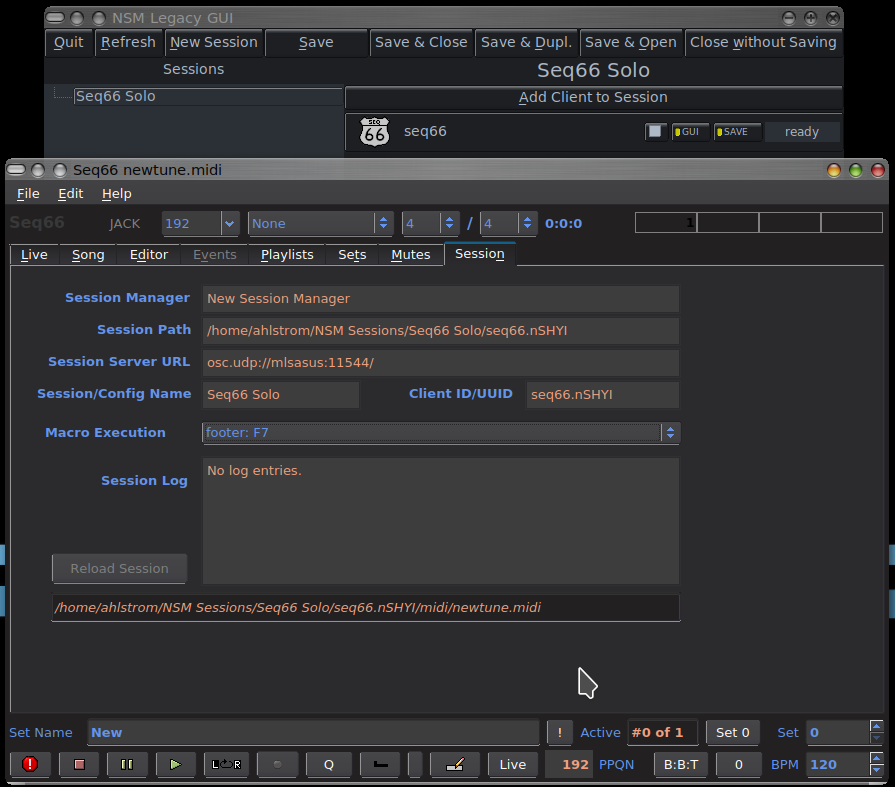
\includegraphics[scale=0.65]{tabs/session/qseq66-session-tab.png}
   \caption*{Session Tab Under NSM}
\end{figure}

   Note that the alternate coloring was set using a Qt style-sheet.
   The next diagram is more up-to-date, and shows the \textbf{Song Info}
   pane for adding a Text event to the song.

\begin{figure}[H]
   \centering 
%  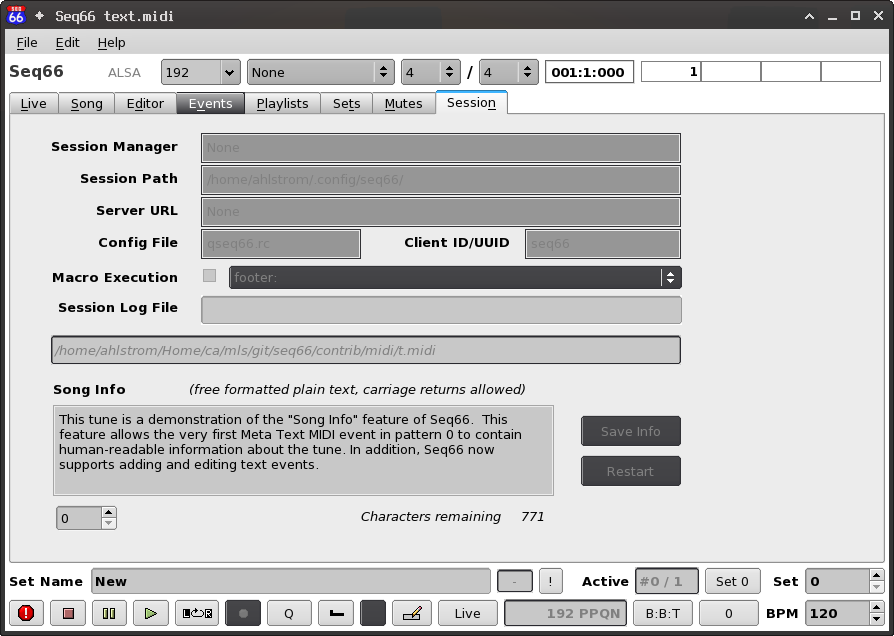
\includegraphics[scale=0.65]{tabs/session/qseq66-session-tab-song-info.png}
   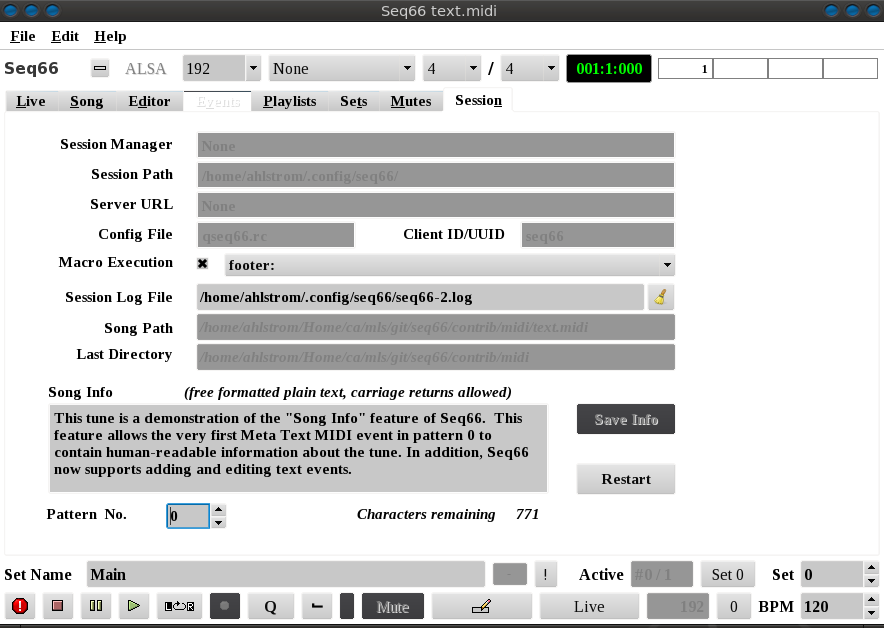
\includegraphics[scale=0.65]{tabs/session/session-song-info.png}
   \caption*{Session Tab with Song Info}
\end{figure}

   \index{sessions!ui}
   This section describes the \textsl{Session} tab in the main
   \textsl{Seq66} window.  This tab displays mostly informative and
   \textsl{read-only} information (except for the name of the log file
   and the editable song-info pane).
   It displays the following bits of information that \textsl{Seq66} has
   received from \textsl{NSM} via the \texttt{nmsd} daemon:

   \begin{itemize}
      \item \textbf{Name} of the session manager.
      \item \textbf{Session path} for the session,
         the root directory of the session.
         All data goes into this directory.
         The name of the directory is of the form
         \texttt{HOME/NSMROOT/SESSIONNAME/UNIQUEID}.
         HOME is the usual UNIX home directory for the user.
         NSMROOT depends on which version of the New/NSM session manager is
         used.
         \index{session!non}
         For the original NSM, this directory is \texttt{NSM Sessions}.
         \index{session!new}
         For the New Session Manager, this directory is
         \texttt{.local/share/nsm}.
         The session name is provided by the user when creating the
         session.
         The unique ID is generated by the NSM.
         If not running in a session,
         the active configuration directory is shown.
      \item The session's \textbf{OSC URL}, which includes the port number.
         Generally, the port number is selected at run-time, but it is also
         possible to configure \textsl{NSM} to use a specific port number.
      \item \textbf{Display name} for the session.
      \item The generated \textbf{client ID} for the session.
      \item \textbf{Macro Execution}.
         This drop-down contains all of the named MIDI macros
         defined in the 'ctrl' file's
         \texttt{[macro-control-out]} section.
         By selecting one, it is automatically sent out via the
         \texttt{[output-buss]} port defined in the 'ctrl' file.
         The "startup" and "shutdown" macros, if defined,
         are sent automatically. "Startup" is useful to put
         a MIDI controller into the proper mode for controlling and displaying
         information in \textsl{Seq66}, and "shutdown" can return the controller
         to its normal operating mode.
      \item \textbf{Session Log File}.The editable name of the log file
         to which to redirect warning
         and error messages during the of action of \textsl{qseq66}.
         Normally, the text is shown in the console window (when running in a
         console window). This name is only a base-name (e.g.
         \texttt{seq66.log}); it is always stored in HOME.
      \item \textbf{Last Directory}.
         Shows the directory from where the last MIDI file was loaded.
      \item \textbf{Restart}.
         \index{restart!manual}
         After editing some of the preferences in the \textbf{Edit / Preferences}
         dialog, one can (later)
         visit this tab and press this button to essentially
         restart \textsl{Seq66}, reloading the new configuration.
         Be careful!
      \item \textbf{Song Info} and \textbf{Pattern No.}.
         \index{song!info}
         \index{meta text}
         This item is a plaintext edit-control that allows the viewing and
         editing of "song info".
         The song info is merely the first Meta Text event, if any,
         found in pattern 0.
         The pattern number can be changed if desired.
         This field can be edited with information such as date, composer,
         playback notes, etc. up to about 1024 ASCII characters.
         Extended ASCII characters are encoded as three hexadecimal
         bytes: "\\xx".
         When the \textbf{Save Info} button is clicked, the meta text
         is copied to the first pattern, thus modifying the file, which
         can then be saved.
   \end{itemize}

   Note that there are many implementations of NSM clients:
   \textsl{Agordejo} \cite{agordejo},
   \textsl{RaySession} \cite{raysession},
   and the
   \textsl{New/Non Session Manager} \cite{nsm}
   with the JACK project's \texttt{nsm-legacy-gui}.

\subsubsection{Seq66 Session Management / NSM / File Menu}
\label{subsubsec:sessions_file_menu}

   The author of \textsl{NSM} has provided documentation for session-management
   which provides very strict instructions on how an application must behave
   under session management.  \textsl{Seq66} tries very hard to stick to these
   instructions.  One major adjustment an application must make is to adhere to
   the "File menu" guidelines.

\begin{figure}[H]
   \centering 
   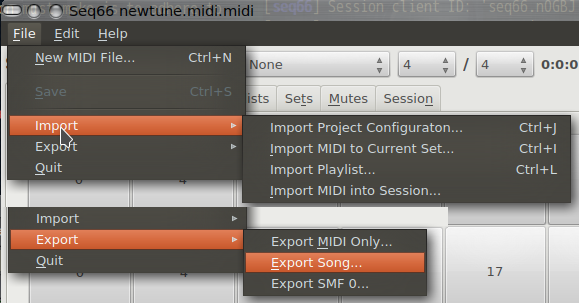
\includegraphics[scale=0.65]{tabs/session/nsm-qseq66-menus-2.png}
   \caption*{File Menu Under NSM, Composite View}
\end{figure}

   Not (yet) shown in the figure are the \textbf{Project Configuration}
   options for import and export.
   (See \sectionref{subsec:menu_file}.)

   This has been changed for 0.98.6; the \textbf{Quit} menu entry becomes
   \textbf{Hide}, as per the NSM protocol.  Also have fixed a bug that disables
   the load-most-recent option under NSM.
   We will update the figure above eventually.
   The following items describe the menu entries.

   \begin{itemize}
      \item \textbf{New MIDI File}.
         This function prompts for the name of a
         new MIDI file and clears the current MIDI file.  The file-name must not
         include a full-path to the file.  The path is hardwired by the
         session.  A relative path can be included.  This name is needed
         because there is no "Save As" option when running in an \textsl{NSM}
         session.
      \item \textbf{Import / Import Project Configuration...}
         Imports a whole project configuration into the current NSM session.
         This functionality used to be automatic (importing the "home"
         configuration), but it is better left to the user to do.
         \index{restart!automatic}
         However, the restart of \textsl{Seq66} after this operation is
         automatic.  Be careful!
      \item \textbf{Import / Import MIDI to Current Set...}
         This action works the same as in normal mode.
         This item allows the user to grab a MIDI file from anywhere and import
         it into the current set.
         The default directory that comes up in the
         prompt is the "last-used directory" from the session 'rc' file.
      \item \textbf{Import / Import Playlist...}
         This action works the same as in normal mode.
         The destination is the NSM session directory.
         \index{restart!automatic}
         Once the playlist is imported,
         \textsl{Seq66} is automatically \textsl{\textbf{restarted}}
         in order to load the playlist.
         Be careful!
      \item \textbf{Import / Import into Session...}
         Prompts the user for a MIDI file to
         be imported (copied) into the current session.  The path to the file
         is then adjusted to use the \textsl{NSM} \texttt{midi} subdirectory.
      \item \textbf{Export / Export Song...}
         Allows exporting the current song as a stock MIDI file, using the
         performance information (triggers) to write the MIDI data as it would
         be played in "song" mode.
         The default directory that comes up in the
         prompt is the "last-used directory" from the session 'rc' file.
      \item \textbf{Export / Export MIDI Only...}
         Allows exporting the current song as a stock MIDI file.
         The "proprietary" SeqSpec data is \textsl{not} written.
         The default directory that comes up in the
         prompt is the "last-used directory" from the session 'rc' file.
      \item \textbf{Export / Export SMF 0...}
         This action works the same as in normal mode.
         It converts the destination file to SMF 0 format.
      \item \textbf{Hide}.
         This menu item replaces the \textbf{Quit} item.
         It hides the main window and tells NSM about it.
   \end{itemize}

   At some point we would like to present a small tutorial showing a session
   under \textsl{JACK}.
   Also note that NSM can invoke or kill applications via
   \textsl{signals}, as explained in 
   \sectionref{subsec:sessions_signals}.

\subsubsection{Seq66 Session Management / NSM / Debugging}
\label{subsubsec:sessions_debugging}

   This section is oriented towards advanced users who found a problem running
   \textsl{Seq66} and want to track it down themselves.  The issue is that we
   need to start the application under the debugger, or start it under NSM and
   somehow attach to \textsl{Seq66} before it starts running.  Another issue is
   that we have found that, at least on the same host, an NSM session
   \textsl{must} be open before \textsl{Seq66} can attach to it, even if the
   correct \texttt{NSM\_URL} is provided.
   So we have to open a session, get the proper URL, configure it in the 'usr'
   file, and then start \textsl{Seq66} under the debugger.
   Here are the steps:

   \begin{enumerate}
      \item Start \textsl{non-session-manager} from a command-line console.
         Write down the URL that it advertises.
      \item Prepare a session for the executable as per earlier instructions.
         Once \texttt{qseq66} starts, immediately exit it, and leave the session
         open.
      \item Open the proper 'usr' file (usually \texttt{qseq66.usr}) in a 
         text editor.  Set variable "session = nsm", and set the variable "url"
         to the value that was advertised.
      \item Now start \texttt{qseq66} in a debugger.
      \item Set a breakpoint in \texttt{clinsmanager::detect\_session()}.
   \end{enumerate}
   
   Now you can step through and see where NSM and Seq66 are getting mixed up.
   Also check the session directory afterward to make the configuration
   (and any MIDI files) are in good shape.

\subsection{Seq66 Session Management / LASH}
\label{subsec:sessions_lash}

   \index{sessions!lash}
   LASH support has been removed.  Use the \textsl{NSM Session Manager} or
   the \textsl{JACK Session Manager}.

\subsection{Seq66 Session Management / sessions.rc}
\label{subsec:sessions_sessions_rc}

   \texttt{Seq66} also supports a more simplistic type of "session",
   where a whole different set of configuration files can be selected.

   One can use the \texttt{--home} and \texttt{--config} options
   to specify alternate locations and names for the configuration files.
   However, if one has a number of configurations
   (e.g. for different sets of equipment. playlists,
   style-sheets, and palettes),
   it's tedious to type these options.
   The \texttt{sessions.rc} file provides a way to set up a
   number of configurations and select one with one option.
   It is always located in the default
   "home" directory, but can refer to directories anywhere. It can also
   specify a different MIDI client-name
   (option \texttt{--client-name})
   and log-file
   (option \texttt{--option log=filename}).

   The user must manually text-edit the sessions.rc to specify tag
   sections like the following:

   \begin{verbatim}
       [test]
       home = "~/.config/seq66/test/"
       config = "test66"
       client-name = "test66"
       log = "test66.log"
   \end{verbatim}

   This section is accessed using the \texttt{-S} or
   \texttt{--session-tag} option, as shown here:

   \begin{verbatim}
       $ qseq66 --session-tag test
   \end{verbatim}

   If this is the first time this command has been run, the
   home directory is created.
   \textsl{Seq66} runs with a MIDI client-name of
   \texttt{test66}.
   The base-name of each configuration file
   is \texttt{test66} (so we have, for example, \texttt{test66.rc)}.
   The log file will be
   \texttt{~/.config/seq66/test/test66.log}.
   (If no log file is wanted, then set it to \texttt{""}.)

   At the end of the run, all of the configuration files are
   saved in 
   \texttt{~/.config/seq66/test/}.
   These can be edited to suit the "test" configuration.
   The setup can also be created via
   \textbf{File / Export / Project configure},
   and then be added to \texttt{sessions.rc}.

   The next time 
   \texttt{qseq66 --session-tag test}
   is run, the test configuration is loaded and used.

   If the specified session tag does not exist in \texttt{sessions.rc},
   then a message is shown; the user should exit \textbf{Seq66} immediately
   and fix \texttt{sessions.rc}.

   Note that the \texttt{log} option overrides the log-file setting
   present in the 'usr' file. Use \texttt{log = ""} to see console output.

%-------------------------------------------------------------------------------
% vim: ts=3 sw=3 et ft=tex
%-------------------------------------------------------------------------------


% Import/Export

%-------------------------------------------------------------------------------
% midi_export
%-------------------------------------------------------------------------------
%
% \file        midi_export.tex
% \library     Documents
% \author      Chris Ahlstrom
% \date        2018-10-20
% \update      2022-01-16
% \version     $Revision$
% \license     $XPC_GPL_LICENSE$
%
%     This section discusses the details of the import/export functionality.
%
%-------------------------------------------------------------------------------

\section{Import/Export}
\label{sec:midi_export}

   This section explains the details of the MIDI import and export
   functionality, accessed by the main menu as noted in sections
   \ref{subsubsec:menu_file_import},
   \ref{subsubsec:menu_file_export}, and
   \ref{subsubsec:menu_file_export_midi_only}, on page
   \pageref{subsubsec:menu_file_import}.

\subsection{File / Import Menu}
\label{subsec:midi_export_file_import_menu}

   The actions for importing files have been move to the new
   \textbf{File / Import} menu in order to keep from cluttering the
   ever-expanding file menu.

\subsubsection{Import MIDI to Current Set}
\label{subsubsec:midi_export_file_import}

   The \textbf{File / Import / Import to Current Set} menu entry imports an SMF 0
   or SMF 1 MIDI file as one or more patterns, one pattern per track, and
   imports them into the currently-active set.
   Even long tracks, that aren't short loops, are imported.
   The difference from \textbf{File / Open} is that the destination screen-set
   (bank) for the import can be specified, and the existing data in the
   already-loaded MIDI file is preserved.
   If the imported file is a
   \textsl{Seq66} MIDI file, it's proprietary sections will
   \textsl{not} be imported, in order to preserve the performance setup.
   The \textbf{Import} dialog is similar to the \textbf{Open} dialog.

   When imported, each track, whether music or information,
   is entered into its own loop/pattern box (slot).
   The import operation can handle reasonably complex files.
   When the file is imported, the sequence number for each track is
   adjusted to put the track into the desired screen-set.
   The import can place the imported data into any of the 32 available
   screen-sets.  Quite large songs can be built by importing patterns.

   Import also handles SMF 0 MIDI files.  It parcels out the SMF 0 data
   into sequences/patterns for each of the 16 MIDI channels.  It also puts
   all of the MIDI data into the 17th pattern (pattern 16), in case it is
   needed.  Note that this slot is used no matter which screen-set one imports
   the file into.  Bug, or feature?
   Also note that, since the file information has been modified by the import,
   the user will be prompted to save the file when exiting \textsl{Seq66}.
   Finally, conversion to SMF 1 for SMF 0 files can be disabled using the
   'usr' option \texttt{[user-midi-settings] convert-to-smf-1}.

\subsubsection{Import Project Configuration}
\label{subsubsec:midi_export_file_import_project}

   This operation allows one to copy all of the \texttt{qseq66.*} configuration
   files from one directory to another.  It is most useful when
   importing a configuration into a new \textsl{NSM} session.
   \index{restart!automatic}
   Once the files are copy, \textsl{Seq66} is automatically restarted,
   in order to load the new configuration.  Be careful!

   Note that the names of the configuration files being impported should
   match the canonical names.  That is, the base names should all be
   \texttt{qseq66} (or \texttt{qpseq66} for \textsl{Windows}.)

\subsubsection{Import Playlist}
\label{subsubsec:midi_export_file_import_playlist}

   This operation allows one to copy a playlist
   from one directory to another.  It is most useful when
   importing a configuration into a new \textsl{NSM} session.
   It copies the playlist file (e.g. \texttt{liveset.playlist})
   into the destination configuration directory.

   Then it creates a subdirectory with the name
   \texttt{playlist/liveset} (for example).
   It then copies all of the MIDI files that were referenced in the
   original playlist into this new directory, preserving
   the directory structure.
   It then wires in and activates the new playlist in the
   'rc' file, and sets the new base directory for the MIDI files.

   \index{restart!automatic}
   Lastly, it restarts \textsl{Seq66}, to load in the new playlist.
   Be careful!

\subsection{File / Export Menu}
\label{subsec:midi_export_file_export_menu}

   The actions for exporting files have been move to the new
   \textbf{File / Export} menu in order to keep from cluttering the
   ever-expanding file menu.

\subsubsection{Export Song}
\label{subsubsec:midi_export_song_export}

   Thanks to \textsl{Seq32}, exporting song performances (see the
   \textbf{Song Editor}) to standard MIDI format has been added.
   The \textbf{File / Export / Export Song} operation modifies the song in the
   following ways:

   \begin{itemize}
      \item Only tracks (sequences, loops, or patterns)
         \index{exportable}
         that are "exportable" are written.  To be exportable, a
         track must have triggers present
         in the \textbf{Song Editor}, and, \textsl{in the song editor}, it
         must not be muted.
      \item Each trigger generates the events, including repeats,
         offset-play of the events, and transposition.
         If there is a gap in the layout
         (e.g. due to an \textbf{Expand} operation in the
         \textbf{Song Editor}),
         then the corresponding gap in the events is exported.
         The result is a track that reconstructs the original
         playback/performance layout of that pattern.
         The events themselves are sufficient to play the performance exactly
         in any MIDI sequencer.
         The triggers are useful for further editing of the song/performance,
         so they are preserved in the triggers \textsl{SeqSpec} section, but
         they cover the whole song.
      \item Empty pattern slots between tracks are removed.
      \item No matter what set the original track was in, it ends up in the
         first set; sets are consolidated.
      \item Other additions, such as time signature and tempo meta events, are
         written in the same manner as for a normal \textbf{File / Save}
         operation.
   \end{itemize}

   The Export dialog is similar to the Open dialog; one will likely want to
   change the name of the file so as not to overwrite it.
   If there are no exportable tracks, the following message is shown:

\begin{figure}[H]
   \centering 
   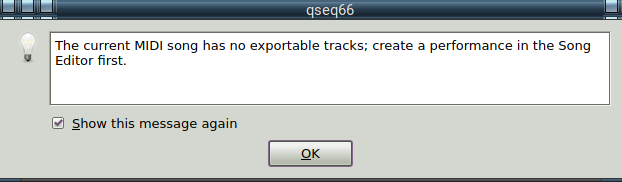
\includegraphics[scale=0.65]{main-menu/file/light-menu-file-song-unexportable.png}
   \caption{MIDI File Unexportable}
   \label{fig:midi_export_file_unexportable}
\end{figure}

   Once the file is exported, reopen it to see the results of the export.
   The following figure shows a before and after picture of the export, as
   seen in the song editor.

\begin{figure}[H]
   \centering 
   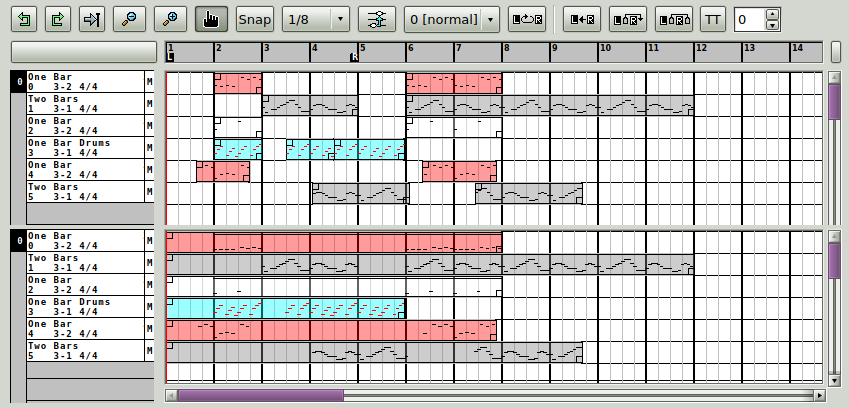
\includegraphics[scale=0.75]{song-editor/song-layout-sample-2.png}
   \caption{MIDI File Layout Before/After Export}
   \label{fig:midi_export_file_before_after}
\end{figure}
   
   The gaps in layouts in the song/performance data are reflected in the
   consolidated triggers.
   Here is the before/after triggers for pattern \#0, which was
   layed out with \textbf{Record Snap} \textsl{on}:

   \begin{verbatim}
       BEFORE                              AFTER
      Sequence #0 'One Bar'               Sequence #0 'One Bar'
      Length (ticks): 768                 Length (ticks): 5375
      trigger: 768 to 1535 at 768         trigger: 0 to 5375 at 5375
      trigger: 3840 to 5375 at 768        
   \end{verbatim}

   Note that 768, at PPQN = 192, is 4 beats (1 measure), while 5375 is 28
   beats (7 measures).
   For each of these triggers, the first number is the start of the trigger in
   PPQNs, the second is the end of the triger, and the third, called the
   "offset", is actually the length of the pattern.
   Note how the "AFTER"
   trigger consolidates the "BEFORE" triggers, starts at time 0, extends to
   the end of the last trigger, and has a length equal to the end of the
   trigger.

   Now here is the before/after triggers for pattern \#5, which was
   layed out with \textbf{Record Snap} \textsl{off}:

   \begin{verbatim}
       BEFORE                              AFTER
      Sequence #5 'Two Bars'              Sequence #5 'Two Bars'
      Length (ticks): 1536                Length (ticks): 6911
      trigger: 2344 to 3879 at 1536       trigger: 0 to 6655 at 6911
      trigger: 4944 to 6655 at 0
   \end{verbatim}

   6655 is a little over 34.5 beats, which is what the bottom grey trigger
   shows.
   6911 is almost 36 beats (9 measures).  Something to figure out.

\subsubsection{Export MIDI Only}
\label{subsubsec:midi_export_file_export_midi_only}

   Sometimes it might be useful to export only the non-sequencer-specific
   (non-SeqSpec) data from a \textsl{Seq66} song.
   For example, some buggy sequencers
   (hello \textsl{Windows Media Player})
   might balk at some SeqSpec item in the song, and refuse to load the MIDI
   file.
   For such cases,
   the \textbf{File / Export / Export MIDI Only} menu
   item writes a file that does not contain
   the SeqSpec data for each track, and does not include all the SeqSpec data
   (such as mute groups) that is normally written to the end of the
   \textsl{Seq66} MIDI file.

\subsubsection{Export SMF 0}
\label{subsubsec:midi_export_file_export_smf_0}

   In some cases it might be useful to convert a \textsl{Seq66} MIDI file to a
   single-track SMF 0 file.
   As with exporting to a song
   (see \sectionref{subsubsec:midi_export_song_export}),
   the tracks to be exported (combined into a single track) must be unmuted
   and have layouts in the song editor.
   The \textbf{File / Export / Export SMF 0 } menu
   action removes all the existing tracks and merges them into track 0.

%-------------------------------------------------------------------------------
% vim: ts=3 sw=3 et ft=tex
%-------------------------------------------------------------------------------


% Configuration files are now consolidated into one file

%-------------------------------------------------------------------------------
% configuration
%-------------------------------------------------------------------------------
%
% \file        configuration.tex
% \library     Documents
% \author      Chris Ahlstrom
% \date        2021-01-18
% \update      2023-10-20
% \version     $Revision$
% \license     $XPC_GPL_LICENSE$
%
%     Provides the configuration information.
%
%-------------------------------------------------------------------------------

\section{Seq66 Configuration}
\label{sec:configuration}

   \textsl{Seq66} configuration has become more elaborate with time, with more
   configuration files.
   Configuration items are well documented in the
   \textsl{Seq66} "man" page and in the configuration files.
   Therefore, this new discussion will merely summarize the options and
   go into a few details about the configuration files.
   Here are the topics to discuss:

   \begin{itemize}
      \item \textbf{Command-line Options}. Useful with desktop shortcuts.
      \item \textbf{'rc' File}. Mostly I/O port options, JACK options, recent
         files.  Also now specifies other files to be used.
      \item \textbf{'usr' File}. Local names for busses and instruments,
         user-interface settings, sessions... Some options that fit either the
         GUI or the command-line application could be moved to the 'rc' file.
      \item \textbf{'ctrl' File}. The keystroke and MIDI control settings have
         been moved to a separate file for flexibility.
      \item \textbf{'mutes' File} The mute-groups settings have
         been moved to a separate file for flexibility.
      \item \textbf{'drums' File}.  This file supports remapping percussion
         notes from older drum machines to General MIDI.
      \item \textbf{'palette' File}. This new file allows replacing the default
         piano-roll, time, data, and events drawing to be tailored.
      \item \textbf{'playlist' File}. This new file specifies a file that
         contains one or more playlists and MIDI controls for them.
      \item \textbf{'qss' File}.  Qt style-sheets can now tailor the appearance
      of theme-drawn elements (e.g. the pattern-grid buttons and text controls).
   \end{itemize}

   After the first run and exit of \textsl{Seq66},
   it generates a set of default configration files in the default
   \textsl{configuration} directory:

   \begin{verbatim}
      /home/user/.config/seq66/qseq66.rc
      /home/user/.config/seq66/qseq66.usr
      /home/user/.config/seq66/qseq66.ctrl
      /home/user/.config/seq66/qseq66.mutes
      /home/user/.config/seq66/qseq66.drums
      /home/user/.config/seq66/qseq66.playlist
      /home/user/.config/seq66/qseq66.palette
   \end{verbatim}

   The palette file is not automatically generated.  It can be saved from the
   \textbf{Edit / Preferences / Display} tab.
   The style-sheet file can be specified in the 'usr' file's "user UI tweaks"
   section.
   There are also some 'keymap' files.  They are not yet used, but may become a
   feature of \textsl{Seq66} in the future.
   For \textsl{Microsoft Windows}, the default base name of the files is
   \texttt{qpseq66}, and the default configuration directory is

   \begin{verbatim}
        C:/Users/user/AppData/Local/seq66/
   \end{verbatim}

   When running \textsl{Seq66} from the \textsl{Non Session Manager}
   (see \sectionref{sec:sessions}),
   the configuration directory is automatically set to something like

   \begin{verbatim}
      /home/user/NSM Sessions/MySession/seq66.nRSIQ/config
   \end{verbatim}

   There is no palette file by default, but the user can create one.
   The color palettes are discussed in \sectionref{sec:palettes}.
   Other files contain the the data for remote MIDI control, computer keyboard
   control, MIDI clock, JACK transport, and a many other settings.
   Some of the settings can be modified in the \textbf{Edit / Preferences}
   dialog, or overridden from the command line.

   \textsl{Seq66} overwrites the most of these files upon exiting.
   One must therefore quit \textsl{Seq66} before making
   manual modifications to these files.

\subsection{Configuration File Commonalities}
\label{subsec:configuration_file_commonalities}

   All of the \textsl{Seq66} configuration files have the following in common:

   \begin{itemize}
      \item \textbf{[Seq66] Section}
      \item \textbf{[comments] Section}
      \item \textbf{Numeric Settings}
      \item \textbf{Boolean Settings}
      \item \textbf{Variables}
      \item \textbf{Stanzas}
   \end{itemize}

   Generally, each configuration file has its own specific set
   of sections, each section-name being enclosed in square brackets in a very
   strict format:  No spaces inside the square brackets.  Sections are looked up
   by this name, including the square brackets, and the name must be exact.

\subsubsection{[Seq66] Section}
\label{subsec:configuration_common_seq66_section}

   This section is informational.  At a minimum, it holds two
   variables:

   \begin{itemize}
      \item \texttt{config-type}.  This value indicates the type of the file,
      such as "ctrl" or 'rc'.
      \item \texttt{version}.  This value indicates the version of the file.
      It is used in some cases when we have added a feature to the
      configuration file that cannot be automatically handled.
      When the internal version number of the file is incremented,
      it can be used to make adjustments for changes in configuration when
      reading older versions of files.
   \end{itemize}

   This section may also contain additional "global"
   variables specific to a given \texttt{config-type}.

\subsubsection{[comments] Section}
\label{subsec:configuration_common_comments_section}

   The "comments" section is also informational, but the user can edit this
   section to include information describing the purpose of the file.  For
   example, a 'ctrl' file for a \textsl{Novation Launchpad} might describe the
   purpose of this file.  The comments stop at the first blank (not even spaces)
   line.  To skip a line in the comment, put a single space character on the
   blank line.

\subsubsection{Numeric Settings}
\label{subsec:configuration_common_numeric_settings}

   Numeric settings consist of a line containing one or more numbers, usually
   preceded by an explanatory comment, and followed by a standard script
   comment.

   \begin{verbatim}
      3    # grid_style       # obsolete, by the way
   \end{verbatim}

   We have been replacing these kinds of settings with the
   \texttt{name = value} style described below, but there are a few places
   where the old style persists, or is more convenient.

\subsubsection{Boolean Settings}
\label{subsec:configuration_common_boolean_settings}

   Boolean settings are the same as numerical settings, but have only
   two values: "0" or "1".

   \begin{verbatim}
      0        # flag to record incoming data by channel
   \end{verbatim}

   We have been trying to replace these kinds of settings with the
   \texttt{name = true/false} style described below, but there are a few places
   where the old style persists.

\subsubsection{Variables}
\label{subsec:configuration_common_variables}

   Variable are a new style of value setting, and can encompass not only
   booleans and numeric values, but string values, which may correspond to
   enumerated values in the source code.  These values are specified by a
   section-name plus variable name/value pair.  Here are some sample
   \texttt{name = value} pairs:

   \begin{verbatim}
      load-mute-groups = true
      save-mutes-to = both
      window-scale = 1.0
      default-ppqn = 1920
      directory = "/home/user/Seq66 files/midi"
   \end{verbatim}

   If the variable value is a string value that is the name of a file or
   directory or path, it must be surrounded with quotes, in case the path has
   spaces in it.

\subsubsection{Stanzas}
\label{subsec:configuration_common_stanzas}

   We have streamlined the control-file stanza by eliminating the "enabled" and
   "channel" columns, since they can be encoded in the event/status
   byte (e.g. 0x90) instead.  Older versions of the 'ctrl' file will be
   upgraded automatically.

   A stanza in a \textsl{Seq66} configuration file consists of some data at the
   beginning, a set of values inside square brackets, and a comment
   at the end.  The values inside the square brackets are numeric, and can
   be in decimal format, hexadecimal format, or binary "0/1" format.
   See \sectionref{subsubsec:configuration_ctrl_loop_control}, which describes
   the details of this layout.

   \begin{verbatim}
      0 "1" [ 0 0x00 0 0 0 ] [ 0 0x00 0 0 0 ] [ 0 0x00 0 0 0 ]  # Loop 0
      1 "q" [ 0 0x00 0 0 0 ] [ 0 0x00 0 0 0 ] [ 0 0x00 0 0 0 ]  # Loop 1
      2 "a" [ 0 0x00 0 0 0 ] [ 0 0x00 0 0 0 ] [ 0 0x00 0 0 0 ]  # Loop 2
      3 "z" [ 0 0x00 0 0 0 ] [ 0 0x00 0 0 0 ] [ 0 0x00 0 0 0 ]  # Loop 3
      . . .
   \end{verbatim}

\subsection{Command Line}
\label{subsec:configuration_command_line}

   Command-line options are well-described in the \textsl{Seq66} "man" page.
   Here, we will present a brief note about each option, and, where applicable,
   a reference to the corresponding configuration file option.
   Here is the basic command line:

   \begin{verbatim}
       qseq66 [options list] [MIDI filename]
   \end{verbatim}

   \optionline{-h}{-{}-help}
      Display a list of all command-line options, then exit.

   \optionline{-V}{-{}-version}
      Display the program version, then exit.

   \optionline{-v}{-{}-verbose}
      During execution, write more information to the console.  Useful for
      trouble-shooting.
   
   \optionline{-n}{-{}-nsm}
      Activate a simple simulation of the built-in NSM
      (\textsl{Non Session Manager}) support, for debugging.
      As of version 0.99.3, \textsl{Seq66} detects if its parent process
      is the \texttt{nsmd} daemon automatically (on Linux).

   \optionline{-T}{-{}-no-nsm}
      Ignore the NSM setting in the 'usr' file. ('T' for 'typical').
      Not too useful at this time.

   \optionline{-X}{-{}-playlist [filename]}
      This option loads the given file-name as a play-list file.
      See \sectionref{sec:playlist}.

      \configref{rc}{playlist}{name}

      \configref{playlist}{playlist}{full}

   \optionline{-m}{-{}-manual-ports}
      \textsl{Seq66} won't attach the system's existing ALSA or JACK MIDI ports.
      Instead, it will create is own set of \textsl{virtual}
      input and output busses/ports.  The default number of port is 1 for input,
      and 16 for output, but these values can be changed in the 'rc' file.

      \configref{rc}{manual-ports}{flag for manual/virtual ports}

   \optionline{-a}{-{}-auto-ports}
      \textsl{Seq66} will automatically attach to the system's existing
      ALSA/JACK ports.

      \configref{rc}{manual-ports}{flag for manual/virtual ports}

   \optionline{-r}{-{}-reveal-ports}
      \textsl{Seq66} will show the names of the ALSA/JACK ports that the system
      defines, rather than the names defined in the 'usr' configuration file.

   \optionline{-R}{-{}-hide-ports}
      \textsl{Seq66} will show the names of the ALSA port that the 'user'
      configuration file define, rather than the names defined by ALSA.

      \configref{rc}{reveal-ports}{flag for reveal ports}

      \configref{usr}{user-midi-bus-definitions}{number of user-defined busses}

   \optionline{-A}{-{}-alsa}
      \textsl{Seq66} will run with ALSA, even if JACK is running.
      This options is "sticky" (they are saved).

   \optionline{-b}{-{}-bus [buss]}
      Modifies the output buss number on \textsl{all} tracks when a MIDI file is
      read. Useful for testing or quick-and-dirty setup, and for adapting a
      playlist to route to a specific MIDI output.

   \optionline{-l}{-{}-client-name}
      Replaces the normal client-name, \texttt{seq66}, with the given name.
      Probably best to make sure "seq66" is part of the name, for clarity.
      Also note that, if active, the \textsl{Non Session Manager} will override
      this name, e.g. using something like \textsl{seq66.nXYZT}.

   \optionline{-q}{-{}-ppqn [ppqn]}
      Supports modifying the PPQN value of Seq66, which is
      defaults to a value of 192.  This setting
      is written into the MIDI file when it is saved.
      The PPQN value can range from 32 to 19200, or
      be set to 0 to use the PPQN from the loaded file.

      \configref{usr}{user-midi-settings}{midi\_ppqn}.

      \configref{usr}{user-session}{session}

   \optionline{-H}{-{}-home [directory]}
      Change the "home" configuration directory from \texttt{\$HOME.config/seq66}
      The configuration files are loaded from or saved to the specified directory.
      If the directory is a full path (such as 
      \texttt{\textasciitilde/test/import}), then
      the directory is used as is.
      If the directory is a simple directory (such as \texttt{test}
      or \texttt{test/import}), then it
      is placed in the normal "home" configuration directory and is used
      to contain the configuration.

   \optionline{-s}{-{}-show-midi}
      Dumps incoming MIDI to the screen.

   \optionline{-p}{-{}-priority}
      Runs at higher priority with a FIFO scheduler.

%  \optionline{n/a}{-{}-pass-sysex}
%     Passes any incoming SYSEX messages to all outputs.
%   Not yet fully implemented.

   \optionline{-k}{-{}-show-keys}
      Prints pressed key value.

   \optionline{-K}{-{}-inverse}
      Changes the color palette for the sequence editor and performance editor
      piano rolls.  Also note that the palette is highly configurable.
      And there is also an option to use a Qt style-sheet.

      \configref{palette}{palette}{inverse}

   The following options can be configured in the 'rc' file. (But note that,
   since version \textsl{Seq66} 0.94.0, the format of that section of the file
   has been simplified.
   See \sectionref{subsubsec:configuration_rc_jack_transport}.

   \optionline{-t}{-{}-jack-midi}
      \textsl{Seq66} will run with JACK, for MIDI if JACK is running.

      \configref{rc}{jack-transport}{jack-midi = true}

   \optionline{-N}{-{}-no-jack-midi}
      \textsl{Seq66} will not run with JACK for MIDI, even if JACK is running.

      \configref{rc}{jack-transport}{jack-midi = false}

   \optionline{-W}{-{}-jack-connect}
      \textsl{Seq66} will connect automatically to JACK ports discovered on the
      system. This is the long-standing default with Seq66.

      \configref{rc}{jack-transport}{jack-connect = true}

   \optionline{-w}{-{}-no-jack-connect}
      \textsl{Seq66} will not automatically connect to other JACK ports.
      This option is useful if a session manager is in charge of the
      connections.
      This option is not available with the other MIDI engines.

      \configref{rc}{jack-transport}{jack-connect = false}

   \optionline{-S}{-{}-jack-slave}

   \optionline{-S}{-{}-jack-slave}
      \textsl{Seq66} will sync to JACK transport as a "slave", if \textsl{JACK}
      is running.

   \optionline{-j}{-{}-jack-transport}
      \index{deprecated}
      This option is the old, \textbf{deprecated} version of
      \texttt{-{}-jack-slave}.

      \configref{rc}{jack-transport}{transport-type = slave}

   \optionline{-g}{-{}-no-jack-transport}
      \textsl{Seq66} will not sync to JACK transport.
      This disables JACK transport if it had been enabled previously.

      \configref{rc}{jack-transport}{transport-type = none}

   \optionline{-J}{-{}-jack-master}
      \textsl{Seq66} will try to be JACK master.

      \configref{rc}{jack-transport}{transport-type = master}

   \optionline{-C}{-{}-jack-master-cond}
      JACK master will fail if there is already a master.

      \configref{rc}{jack-transport}{transport-type = conditional}

   \optionline{-M}{-{}-jack-start-mode [x]}
      When \textsl{Seq66} is synced to JACK, the following play modes
      are available: "live" = live mode; "song" = song mode, and "auto" means
      use song mode if triggers are present in the loaded MIDI file. "auto" is
      the default.

      \configref{rc}{jack-transport}{song-start-mode = auto}

   \optionline{-U}{-{}-jack-session-uuid [uuid]}
      Set the UUID for the JACK session.  This value is useful when
      running \textsl{Seq66} from within a \textsl{JACK} session.
      The session controller (e.g. \textsl{QjackCtl}) uses this value in the
      command-line when starting \textsl{Seq66}.
      See \sectionref{subsec:sessions_jack}.

   \optionline{-0}{-{}-smf-0}
      Normally, SMF 0 (single-track MIDI) files are split into separate tracks
      when read into Seq66.  This 'usr' option preserve the file as an SMF 0
      file.

   \optionline{-u}{-{}-user-save}
      Save the 'usr' configuration file when exiting.
      Normally, it is saved only if not present in the configuration directory,
      so as not to get stuck with temporary settings such as the -{}-bus option.

      \configref{rc}{auto-option-save}{auto-save-rc}

   \optionline{-f}{-{}-rc filename}
      Use a different 'rc' configuration file.
      It must be a file in the user's \texttt{\$HOME/.config/seq66}
      directory or the directory specified by the \texttt{-{}-home} option.
      The \texttt{.rc} extension is added if necessary.

   \optionline{-F}{-{}-usr filename}
      Use a different 'usr' configuration file.  Similar to the \texttt{-{}-rc}
      option. But note that this can be controlled in the 'rc' file as
      well.

   \optionline{-c}{-{}-config basename}
      Use a different configuration file base name for the 'rc' and 'usr'
      files.  For example, one can specify a full configuration for "testing",
      for "jack", or for "alsa", to set up
      \texttt{testing.rc} and \texttt{testing.usr},
      \texttt{jack.rc} and \texttt{jack.usr},
      \texttt{alsa.rc} and \texttt{alsa.usr}.
      But note that recent versions of \textsl{Seq66} use the 'rc' file
      to control the names and active state of all the other configuration
      files.

   \optionline{-L}{-{}-locale localename}
      Set a different locale for running \textsl{Seq66}.
      If the current locale uses the comma as a decimal point,
      then try to use \texttt{en\_US.UTF-8} (for example).

   \optionline{-o}{-{}-option opvalue}
      Provides additional options, since the application is running out of
      single-character options.  The \texttt{opvalue} set supported is:
      \begin{itemize}
         \item \texttt{daemonize} and \texttt{no-daemonize}.
            \index{daemonize}
            Sets up the \texttt{seq66cli} application to fork to the background
            the \textsl{next time} it is run.
            This is done by modifying the \texttt{seq66cli.usr}
            file to specify daemon runs.
            It is good to specify a log-file as well.
            \index{no-daemonize}
            undoes the setup of \texttt{seq66cli} daemonization.
            The application can then be run in
            a console so that log output can be seen.
         \item \texttt{log=filename.log}.
            \index{log}
            Reroutes standard error and standard
            output messages to a log-file located in
            the configuration directory.
            If this file is present, log information is appended.
            The default log-file name is specified in the
            \texttt{[user-options]} section of the 'usr' file.
            If using daemonization, it pays to also set up a log
            file with the same command.
         \item \texttt{sets=8x8}.
            \index{variset}
            This option, informally known as "variset", allow some changes in
            the set size and layout from the default 4x8 = 32 sets layout.
            Consider this option to be experimental.
            Expect problems (and please report them).
            To save these options to the 'usr' file, add the
            \texttt{-{}-user-save} option to the command line, or edit the
            'usr' file before running \textsl{Seq66}.
            In that file, the options modified are \texttt{mainwnd\_rows} and
            \texttt{mainwnd\_cols}.
         \item \texttt{scale=WxH}.
            \index{scaling}
            This option scales the main window by the given factors,
            ranging from 0.5 to 3.0. A 1920x1080 screen can be completely
            filled via \texttt{-{}-option scale=2.175x1.75}. Even when scaled 
            down, the user can use the mouse of window-manager keystrokes to
            shrink the window even further.
            Note that the other tabs in the main window do not adjust
            appropriately... this feature is meant for live usage of
            a touch-screen.
         \item \texttt{mutes=value}. Specifies the saving of mute-groups
            to the 'mutes' file, 'midi' file, or 'both' files.
         \item \texttt{virtual=o,i}. Set up the manual-ports option with 'o'
            output ports and 'i' input ports.
      \end{itemize}

\subsection{'rc' File}
\label{subsec:configuration_rc}

   \begin{verbatim}
      /home/user/.config/seq66/qseq66.rc
   \end{verbatim}

   The 'rc' configuration file has undergone a lot of changes, including
   off-loading the keyboard control, MIDI control, and mutes control sections
   into their own files, and adding a few "variable" settings.
   Rather than repeating information already present in the self-documenting
   'rc' file, we will summarize the settings and refer the reader to the sample
   files for more information.

   The 'rc' file adds these \texttt{[Seq66]} options to the common
   data for all configuration files:

   \begin{verbatim}
      sets-mode = normal
      port-namng = short
   \end{verbatim}

   \index{sets-mode}
   The \texttt{sets-mode} option determines how patterns are muted when the
   play-screen (current set) changes.  Its values are:

   \begin{itemize}
      \item \textbf{normal}.
      \index{sets-mode!normal}
         When moving to another set, the patterns in the
         current play-screen are muted, as are the patterns in the destination
         set.
      \item \textbf{autoarm}.
      \index{sets-mode!autoarm}
         Similar to normal, but the patterns in the
         destination set are automatically unmuted.
      \item \textbf{additive}.
      \index{sets-mode!additive}
         When moving to another set, the destination set
         is added to the play-set, so that both sets are playing.
         This option was requested by users.
      \item \textbf{allsets}.
      \index{sets-mode!allsets}
         When a song is loaded, all patterns in all sets are unmuted and will
         play.
   \end{itemize}

   \index{port-naming}
   The \texttt{port-naming} option determines how much detail is shown in
   port names as shown in the user-interface.  It does not apply if
   port-mapping (\sectionref{sec:port_mapping}) is active (and note that
   port-mapping is now the default).
   Port-naming values are:

   \begin{itemize}
      \item \textbf{short}.
      \index{port-naming!short}
         The brief name is shown; this is just the bare device name.
      \item \textbf{pair}.
      \index{port-naming!pair}
         The ALSA client number and port are shown along with the device name.
         Example "128:0 VMPK Input"
      \item \textbf{long}.
      \index{port-naming!long}
         The internal number of the clients and ports are shown.
         These are a sequence of port numbers: 0, 1, 2, 3, etc.
   \end{itemize}

   For \textsl{Windows} (the "portmidi" build),
   the 'long' option works better.

\subsubsection{'rc' File / MIDI Control}
\label{subsubsec:configuration_rc_midi_control}

   \index{[midi-control-file]}
   \textsl{Seq66} offloads MIDI control to a separate file.
   Move or create
   the \texttt{[midi-control]} section to a separate file in
   the \textsl{Seq66} configuration directory, and add the following
   snippet:

   \begin{verbatim}
      [midi-control-file]
      active = true           # true means to use and to rewrite at exit
      name = "qseq66.ctrl"    # contains a [midi-control] section, and more
   \end{verbatim}

   As with the 'rc' file, the 'ctrl' file can be rewritten upon exit,
   \textsl{except} that it is not written unless it is \textsl{active},
   or \textsl{does not exist} (as during the first run of \textsl{Seq66}).
   For the details of the 'ctrl' file, see
   \sectionref{subsec:configuration_ctrl}.

\subsubsection{'rc' File / Mute Groups}
\label{subsubsec:configuration_rc_mute_groups}

   The 'rc' file has been modified so that mute-group are now stored in a
   separate file.  The following section specifies that file, which should be
   located in the session/configuration directory.

   \begin{verbatim}
      [midi-group-file]
      active = false
      name = "qseq66.mutes"   # contains a [mute-groups] section
   \end{verbatim}

   The mutes-groups themselves are loaded from the 'mutes' file dependent on
   the \texttt{load-mute-groups} option in the mute-groups file.
   The mutes-groups section is written on exit dependent on the
   \texttt{save-mutes-to} option in the mute-groups file.
   It can go to the MIDI file, the 'mutes' file, or both.

\subsubsection{'rc' File / Color Palette}
\label{subsubsec:configuration_rc_color_palette}

   \begin{verbatim}
      [palette-file]
      active = false
      name = "qseq66.palette"
   \end{verbatim}

   The only need for a palette file is when not satisfied with the
   default palette for the patterns, inverse colors, hatching,
   or grid-lines for some pattern piano roll items.
   There is a button to save the current/default
   palette for later modification in the \textbf{Edit / Preferences / Display}
   tab.

\subsubsection{'rc' File / Note Mapper}
\label{subsubsec:configuration_rc_note_mapper}

   \begin{verbatim}
      [note-mapper]
      active = false
      name = "GM_DD-11.drums"
   \end{verbatim}

   This file can be used transform the existing drum (non-transposable) tracks
   into another set of drum tracks.  A lot of work has been done in the past
   with non-General-MIDI instruments (particularly consumer instruments like the
   \textsl{Yamaha PSS-780} or \textsl{Yamaha DD-11}.
   This option is useful for transformation older MIDI files into GM format.
   For the usage of the note-mapper, see
   \figureref{fig:pattern_editor_oneshot_recording}, and the surrounding
   discussion.

\subsubsection{'rc' File / MIDI-Clock Section}
\label{subsec:configuration_rc_midi_clock}

   \index{[midi-clock]}
   The MIDI Clock tab contains the clocking state from the last 
   time \textsl{Seq66} was run, their status, and their names.
   It also specifies the MIDI output ports, which can be disabled.
   Disable the port with a -1, turn off the clock with a 0,
   or turn it on with a 1 (which means to send
   \textbf{MIDI Song Position}, and
   \textbf{MIDI Continue} if
   starting after tick 0), or on with positioning with a 2, which sends
   \textbf{MIDI Start}
   and then begins clocking after the position reaches a modulo of the
   \textbf{Clock Start Modulo value}.  Luckily, the user-interface makes it
   easy to select the desire value, and has tool-tips to instruct the user.
   This configuration item is represented in the
   \textbf{Edit / Preferences / MIDI Clock} tab.

   \begin{verbatim}
      [midi-clock]
      5    # number of MIDI clocks (output busses)
      0 0    "[0] 14:0 Midi Through Port-0"
      1 0    "[1] 128:0 TiMidity port 0"
      2 0    "[2] 128:1 TiMidity port 1"
      . . .
   \end{verbatim}

   If there are USB MIDI devices plugged in (on \textsl{Linux} using JACK),
   they will show up with system names that have no meaning to the user.
   In this case, an "alias" looked up by JACK is appended as a comment in the
   'rc' files, and also shows up in the port lists in the user interface.
   For example:

   \begin{verbatim}
      0 0    "[0] 0:0 system:midi_capture_1"        # Midi-Through
      1 1    "[1] 0:1 seq66:system midi_capture_5"  # Launchpad-Mini
      2 0    "[2] 0:2 system:midi_capture_3"        # USB-Midi
      3 0    "[3] 0:3 system:midi_capture_4"        # nanoKEY2
   \end{verbatim}

   Note the difference in naming of the enabled port (Launchpad-Mini).
   The appended label is \textsl{not} part of the port name;
   it is there simply to help the user select the correct system port.
   This same setup applies to MIDI input ports as well.
   Note that the 'rc' file has a port-mapping option, described elsewhere.

   Ports created by \texttt{a2jmidid --export-hw} do not have JACK aliases.
   Ports created by Seq66 do not have JACK aliases.  Ports created by MIDI
   applications such as \textsl{Qsynth} do not have JACK aliases. Ports
   created by ALSA or \textsl{Windows} do not have aliases.

   On some recent \textsl{Linux} systems,
   these USB system ports can be accessed without
   exposing the ports via \texttt{a2jmidid}, since JACK does it.
   One can see all the aliases on a JACK setup with the following
   command:

   \begin{verbatim}
      $ jack_lsp --aliases
   \end{verbatim}

   For output port-mapping, which is now the default for \textsl{Seq66},
   see \sectionref{subsec:output_port_mapping}.

\subsubsection{'rc' File / MIDI Clock Mod Ticks}
\label{subsubsec:configuration_rc_midi_cmt}

   \index{[midi-clock-mod-ticks]}
   This configuration item is the same as the
   \textbf{Edit / Preferences / MIDI Clock / Clock Start Modulo} option.

   \begin{verbatim}
      [midi-clock-mod-ticks]
      ticks = 64
      record-by-channel = false
   \end{verbatim}

   The record-flag should be in the 'usr' file;
   something to rectify later.

\subsubsection{'rc' File / MIDI-Meta-Events Section}
\label{subsubsec:configuration_rc_midi_meta_events}

   \index{[midi-meta-events]}
   The MIDI Meta events section is the start of additional options
   supporting meta events as normal events in \textsl{Seq66};
   it defines only the tempo MIDI meta-event at present.
   Normally, tempo events are supposed to occur in the first track (pattern 0).
   But one can move this track elsewhere to accomodate one's existing body of
   tunes.  It affects where tempo events are recorded.  The default value is 0,
   the maximum is 1023.  A pattern must exist at this number for it to work.
   \index{tempo-track-number}

   \begin{verbatim}
      [midi-meta-events]
      tempo-track = 0
   \end{verbatim}

   As per the MIDI specification, the first track (track 1 in track
   numbering, or pattern 0 in \textsl{Seq66} numbering) is \textsl{the}
   official track for certain MIDI meta events, such as
   \textbf{Set Tempo} and
   \textbf{Time Signature}.
   But we allow the user to and change the tempo track to another pattern.

\subsubsection{'rc' File / MIDI Input}
\label{subsubsec:configuration_rc_midi_input}

   \index{[midi-input]}
   This configuration item is represented in the
   \textbf{MIDI Input} tab in the \textbf{Edit / Preferences}.
   The first number is a line count, and equals the number of
   supported input ports.
   After that, this 'rc' entry here has two variables;
   the first is the port number,
   and the second number indicates whether it is disabled (0), or enabled (1).
   The next lines show the input busses present on the system (normally).

   \begin{verbatim}
      [midi-input]
      2   # number of MIDI busses
      0 1    "[0] 0:1 system:announce"
      1 0    "[1] 14:0 Midi Through Port-0"
      2 0    "[2] 28:0 nanoKEY2 MIDI 1"
      3 0    "[3] 48:0 Launchpad Mini MIDI 1"
   \end{verbatim}

   Note that the "system:announce" buss is present only for ALSA, not for JACK.
   This will change the port numbering.
   Again, see the 'rc' file itself for more information.

   \index{linux!system MIDI Thru}
   \index{MIDI Thru}
   One minor issue with the system MIDI Thru port is that, if it and another
   input port (e.g. VMPK) are both enabled, then each note emitted by VMPK is
   doubled. Be aware.

   For input port-mapping, which is now the default for \textsl{Seq66},
   see \sectionref{subsec:input_port_mapping}.

\subsubsection{'rc' File / Manual (Virtual) Ports}
\label{subsubsec:configuration_rc_manual_ports}

   The name of this setting is a bit of a misnomer in a couple of ways:

   \index{ports!virtual}
   \index{ports!manual}
   \begin{enumerate}
      \item It refers to the usage of \textsl{virtual} MIDI ports.
         These are ports set up by the application so that other
         devices, applications, or session managers can connect
         \textsl{manually} to the MIDI application.
      \item This option is not just for ALSA.  It can also be used when
         running in native JACK mode, to support
         virtual JACK ports that can be connected manually (e.g. in the
         \textsl{QJackCtl} application.)
   \end{enumerate}

   \index{[manual-ports]}
   \begin{verbatim}
      [manual-ports]
      virtual-ports = false   # 'true' = manual (virtual) ALSA or JACK ports
      output-port-count = 8   # number of manual/virtual output ports
      input-port-count = 4    # number of manual/virtual input ports
   \end{verbatim}

   \index{--auto-ports}
   The opposite of \texttt{-{}-manual-ports} is \texttt{-{}-auto-ports},
   which is the normal mode of running \textsl{Seq66}.
   In this mode, system MIDI input/output devices are discovered and
   automatically connected.
   It will create port names as per the settings in the 'usr' configuration
   file's sections:

   \begin{verbatim}
      [user-midi-bus-definitions]
      [user-midi-bus-N]
   \end{verbatim}

   These definitions can be used by JACK for connection, and these
   definitions can be used to specifically rename the ports that exist in the
   system. (Roughly similar to the MIDInam feature, but not compatible.)
   This option is misleading if one wants to have access to the
   actual ALSA/JACK ports that exist on the system.
   The next option gets around that issue.

\subsubsection{'rc' File / Port Map}
\label{subsubsec:configuration_rc_port_map}

   The 'rc' file also supports a port map, which maps I/O ports from a
   permanent buss number to the actual system buss number.
   The pattern is set to output to a specific buss number; this buss number is
   associated with a port name; this port name is looked up to see what
   system buss number is the one to be used.  When the system setup changes,
   the pattern does not need to changed; only the port mapping may need to be
   changed.  If the port map covers all I/O ports ever possible on a system, it
   will not need to be changed.  See \sectionref{sec:port_mapping}; it contains
   more details.

\subsubsection{'rc' File / Keyboard Control Section}
\label{subsubsec:configuration_rc_keyboard_control}

   The keyboard control section has been merged into the MIDI control section
   and been moved into the 'ctrl' file.
   See \sectionref{subsec:configuration_ctrl}.
   There is no user-interface to change the
   keyboard control, for two reasons:
   (1) It is pretty easy to read, understand, and edit the 'ctrl' file, and
   (2) There are many more controls in \textsl{seq66}, and creating a
   user-interface to edit them might not be worth the effort.
   We suspect most users will be happy enough with the default settings,
   and users of internationaly keyboards will find the 'ctrl' file easy enough
   to edit with a programmer's editor.  As an example,
   \index{keys!AZERTY}
   see \texttt{qseq66-azerty.ctrl} in the \texttt{data/linux}
   directory.
        
\subsubsection{'rc' File / JACK Transport}
\label{subsubsec:configuration_rc_jack_transport}

   This section holds the settings for both JACK transport and for native JACK
   MIDI mode.
   \index{[jack-transport]}
   The JACK Transport options are also command-line options.
   See \sectionref{subsec:configuration_command_line}.
   For \textsl{Seq66} \textsl{before} 0.94.0, a number of boolean digit settings
   were used.
   For \textsl{Seq66} \textsl{after} 0.94.0, the settings are more elegant.

   \begin{verbatim}
      [jack-transport]
      transport-type = slave    # 'none', 'slave', 'master', or 'conditional'
      song-start-mode = song    # 'song' = 'true' or 'live' = 'false'
      jack-midi = true          # 'true' or 'false'
      jack-auto-connect = true  # 'true' or 'false', default is true
   \end{verbatim}

   'conditional' value tells \textsl{Seq66} to try to
   become JACK Master.  If a master already exists, then \textsl{Seq66} falls
   back to JACK Slave.
   Note that JACK transport is separately configurable from
   JACK MIDI. Transport and MIDI use different JACK clients internally.

   \texttt{song-start-mode} is set to 'true' or 'song' to force the usage of the
   track layout in the song editor (see \sectionref{sec:song_editor}).
   If 'false' or 'live' then the live mode is in force, where the musician
   controls the arming of sequences.
   If 'auto', then the mode is set to 'song' if the loaded file has
   a track layout (triggers), and 'live' otherwise.
   It is probably best to leave it at 'auto'.

   \texttt{jack-midi} set to 'true' turns on the usage of JACK for MIDI
   playback.  If running in normal (not "manual/virtual" port) mode,
   then \textsl{Seq66} connects automatically to all JACK MIDI ports it
   finds on the system at startup.

   \texttt{jack-auto-connect} is normally set to 'true'.  If set to false, then
   the automatic connect discussed in the previous paragraph will not be
   performed.
   This option is useful if one want to rely on a session manager to make the
   connections, or do it onself, without using the manual/virtual port feature.

\subsubsection{'rc' File / Reveal Ports}
\label{subsubsec:configuration_rc_reveal_ports}

   This option applies to both ALSA and JACK.

   \index{[reveal-ports]}
   \begin{verbatim}
      [reveal-ports]
      show-system-ports = true   # flag for reveal ALSA ports
   \end{verbatim}

   \index{jack!reveal-ports}
   Turning on the reveal-ports option is necessary if one
   wants to see the actual port names defined by the system.
   It ignores the settings in the 'usr' configuration file's
   \texttt{user-midi-bus-definitions} and \texttt{user-midi-bus-N} sections.
   If this option is turned on, the definitions in the
   'usr' configuration file are \textsl{not} read from that file.

\subsubsection{'rc' File / Metronome}
\label{subsubsec:configuration_rc_metronome}

   A very configurable metronome is supported.
   After running \textsl{Seq66} and then
   exiting, the following section is present:

   \begin{verbatim}
      [metronome]
      output-buss = 1
      output-channel = 0
      beats-per-bar = 4
      beat-width = 4
      main-patch = 0
      main-note = 72
      main-note-velocity = 120
      main-note-length = 0
      sub-patch = 0
      sub-note = 60
      sub-note-velocity = 84
      sub-note-length = 0
      count-in-active = false
      count-in-measures = 1
      count-in-recording = true
      recording-buss = 2
      recording-measures = 0
   \end{verbatim}

   The \texttt{main} settings apply to the first note of the metronome.
   The type of tone is given by the patch (program) number.
   The actual note is given by a MIDI note number.
   The velocity can be set.
   The note-length is controlled by a scale factor:  0 means an automatic
   calculation based on the beat width which equates to a value of 0.5;
   1.0 means the note length is exactly equal to the beat width.
   The minimum is 0.125, and the maximum is 2.0.
   Try different values and see.

   The \texttt{sub} settings apply to the rest of the notes of the metronome,
   but are otherwise the same.
   The settings \texttt{count-in-active} and \texttt{count-in-measures}
   control metronome count-in, where the metronome starts playing before the
   song.
   The rest of the settings are discussed in the following section on
   \textbf{Background Recording}.

   There is a user-interface in
   \textbf{Edit / Preferences} to configure the settings of the metronome (and
   the recorder).
   See \sectionref{paragraph:menu_edit_preferences_metronom_options}.

\subsubsection{'rc' File / Background Recording}
\label{subsubsec:configuration_rc_background_recording}

   Background recording allows recording to be made without having to create a
   pattern and turn on recording.
   It is useful when using a metronome and count-in measures.
   The following settings activate this feature
   and determine the input port to be used.

   \begin{verbatim}
      [metronome]
      . . .
      count-in-recording = true
      recording-buss = 2
      recording-measures = 0
   \end{verbatim}

   The \texttt{count-in-recording} setting enables/disables background recording.
   The \texttt{recording-buss} setting specifies the input buss/port.
   That buss \textsl{must be enabled} (in the 'rc' file).
   The \texttt{recording-measures} sets the number of measures to record.
   The style of recording is currently \textsl{merge},
   where notes accumulate as each loop occurs.
   We might adjust that feaure per user feedback.
   If \texttt{recording-measures} is set to 0, then the
   \textsl{expanding} mode of recording is used, where
   the background-recording sequence gets longer and longers
   as playback and playing continues.

\subsubsection{'rc' File / Interaction Method}
\label{subsubsec:configuration_rc_interaction}

   \begin{verbatim}
      [interaction-method]
      snap-split = false
      click-edit = true
   \end{verbatim}

   The \texttt{Mod4} ("Windows" key) option is no longer available, and not
   necessary.
   Also removed is the option for the "fruity" option of \textsl{Seq24}.
   It will be added back if there is a clamor for it.

   \index{[snap-split]}
   \index{new!snap-split}
   This option comes from the \textsl{seq32} project.  It allows for
   pattern-splitting in the Song editor at snap points, rather than just
   at the middle of the pattern.

   \index{[allow-click-edit]}
   \index{new!allow-click-edit}
   This option allows one to enable/disable the ability to double-click
   in a pattern slot in the main window to bring it up for editing.
   This can interfere with a live performance where muting/unmuting come fast
   enough to be seen as a double-click.

\subsubsection{'rc' File / Auto Option Save}
\label{subsubsec:configuration_rc_auto_option_save}

   \index{[auto-option-save]}
   This item determines if the 'rc' configuration file (and other files)
   is saved upon exit of \textsl{Seq66}.
   The normal behavior is to save it,
   which can sometimes be inconvenient when one is just trying out some
   command-line options.

   \begin{verbatim}
      [auto-option-save]
      auto-save-rc = true
      save-old-triggers = false
      save-old-mutes = false
   \end{verbatim}

   The 'save' options can be set to true to save triggers in the old formats.
   \textsl{Seq66} now saves triggers with a "transpose" value, so that
   clips can be transposed in the song editor for more extensive re-use
   (see the "Kraftwerk" MIDI file for an example).
   The 'mutes' are now save as a single byte, rather than a 4-byte value, to
   save some space.

\subsubsection{'rc' File / Last Used Directory}
\label{subsubsec:configuration_rc_last_used_dir}

   The following item refers to the last directory in which one opened or
   saved a MIDI file.

   \index{[last-used-dir]}
   \begin{verbatim}
      [last-used-dir]
      "/home/user/seq66/contrib/midi/"
   \end{verbatim}

\subsubsection{'rc' File / Recent Files}
\label{subsubsec:configuration_rc_recent_files}

   The following item preserves a list of the last few MIDI files loaded.
   It is not filled when a MIDI file is loaded via a play-list.
   The first number is the count of recent-files.
   The second number is a boolean to determine if the most-recent file
   should be loaded when \textsl{Seq66} starts.
   This option is useful as part of restoring a session.

   \index{[recent-files]}
   \begin{verbatim}
      [recent-files]
      count = 2
      load-most-recent = true
      "/home/user/seq66-alternate/contrib/midi/2Bars.midi"
      "contrib/midi/b4uacuse-seq24.midi"
   \end{verbatim}

\subsubsection{'rc' File / Play-List}
\label{subsubsec:configuration_rc_playlist}

   This item provides a configured set of named play-lists in a play-list file,
   and a flag to activate it.
   Having a playlist makes it easy to load song after song from pre-determined
   lists.
   
   \index{[playlist]}
   \begin{verbatim}
      [playlist]
      active = false
      "/home/user/.config/seq66/sample.playlist"
   \end{verbatim}

   See \sectionref{sec:playlist}.
   It describes the setup, layout, and usage of a
   \textsl{Seq66} playlist file containing one or more playlists.

\subsection{'usr' File}
\label{subsec:configuration_usr}

   This section describes the \textsl{Seq66} 'usr' (or "user") file.
   The main part of the \textsl{Seq66} 'usr'
   configuration file provides a way to give more
   informative names to the MIDI busses, MIDI channels, and MIDI controllers of
   a given system setup.
   This configuration overrides the default values
   of the \textbf{Event} drop-down list and the menu items in the pattern editor,
   and makes them reflect the names of the MIDI Control (CC) values of one's
   devices.

   In \textsl{Seq66} it, also includes some items that affect the
   user-interface's look, and many other new configuration items.
%  At some point we will likely split this file into another configuration file
%  ("qseq66.ui"?)

   \index{qseq66.usr}
   After one runs \textsl{Seq66} for the first time (or after deleting
   the configuration files), it will generate a
   \texttt{qseq66.usr} file in one's "HOME" directory:

   \begin{verbatim}
      /home/user/.config/seq66/qseq66.usr             (Linux)
      C:/Users/user/AppData/Local/seq66/qpseq66.usr   (Windows)
   \end{verbatim}

   In a session manager, the files will be created in the session directory.
   \index{usr!-u}
   \index{usr!--user-save}
   Unlike the 'rc' file, the 'usr' file is \textsl{not} written every time
   \textsl{Seq66} exits.  If the 'usr' files does not exist, one is
   created, but it is normally not overwritten thereafter.
   The important exception is if we have updated the 'usr' file with new option
   and have incremented the version number of this file.
   To cause it to be overwritten at exit, run \textsl{Seq66} with the
   \texttt{-u} or \texttt{-{}-user-save} option:

   \begin{verbatim}
      $ qseq66 --user-save
   \end{verbatim}

   This option is recommended when one installs a new version of
   \textsl{Seq66}, which might add new options to the 'usr' file.
   One usually must edit the 'usr' file manually.
   There are a few items that can be tweaked in \textbf{Edit / Preferences},
   and, if modified, the user-save flag is turned on.

   By default, the list of MIDI devices that \textsl{Seq66} shows depends
   on one's system setup and whether the manual-port option is specified
   or not.  Here's our system, with the
   the \texttt{[manual-port]} option turned off, shown in a
   composite view with all menus one can look at for MIDI settings:

\begin{figure}[H]
   \centering 
   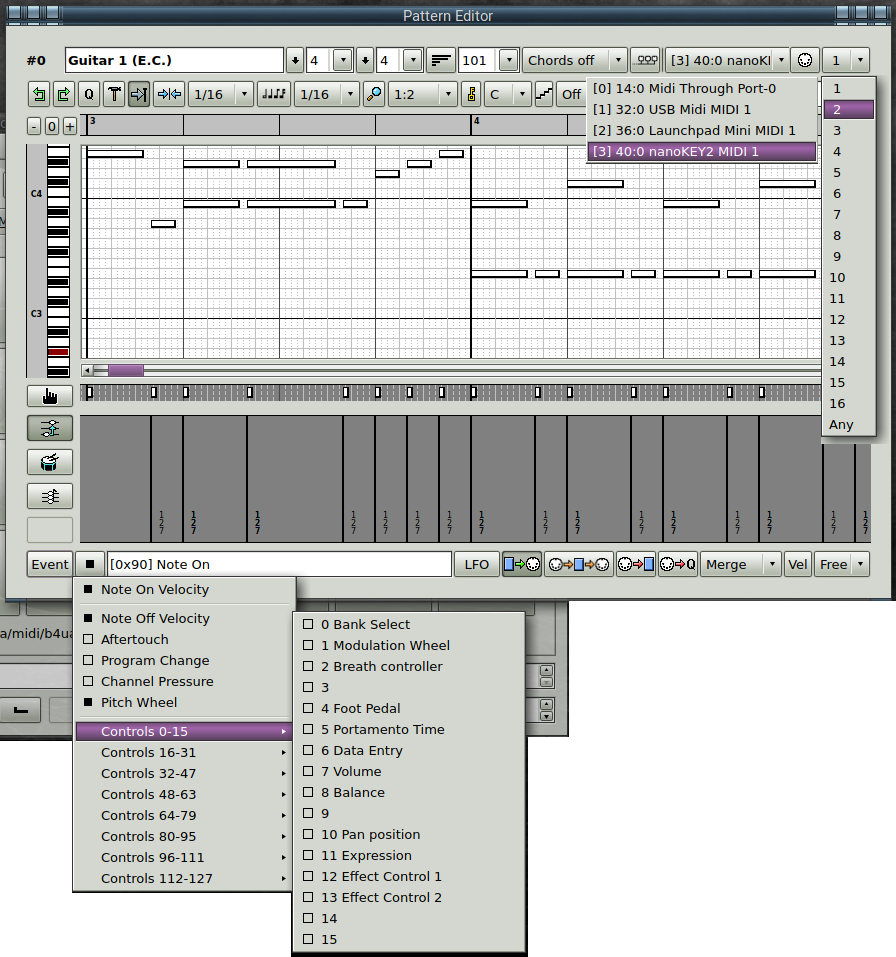
\includegraphics[scale=0.75]{configuration/usr/default-event-bus-channel-menus.png}
   \caption{Seq66 Composite View of Native Devices}
   \label{fig:default_event_bus_channel_menus}
\end{figure}

   At the top, the buss dropdown menu contains the MIDI busses/ports
   active on this computer.  At right, the MIDI channel shows
   the channels numbers that can be picked for buss 0.  At bottom left, we see
   the default controller values that \textsl{Seq66} includes.  We have
   no idea if these correspond to the controllers that the selected MIDI device
   supports.  We \textsl{can} use this dropdown to see if any such controller
   events are in the loaded MIDI file, of course; a solid black square
   indicates that such an event was found in the pattern.

   To change the default lists, we can create sections for busses and
   instruments in the 'usr' file.
   The discussion here relies on the reader opening the file
   \texttt{sample.usr}, which is included in the shared \texttt{data/samples}
   directory provided once \textsl{Seq66} is installed.

   Assume that we have 3 MIDI "buss" devices hooked to our system:
   two Model "2x2" MIDI port devices, and an old PCR-30 MIDI controller
   keyboard.  Let's number them, using the convention that buss numbers and
   channel numbers start at 0, not 1:

   \begin{itemize}
      \item 0. Model 2x2 A
      \item 1. Model 2x2 B
      \item 2. PCR-30
   \end{itemize}

   Then assume that we have nine different MIDI instruments in our kit.
   let's number them, too:

   \begin{itemize}
      \item 0. Waldorf Micro Q
      \item 1. SuperNova
      \item 2. DrumStation
      \item 3. TX81Z
      \item 4. WaveStation
      \item 5. ESI-2000
      \item 6. ES-1
      \item 7. ER-1
      \item 8. TB-303
   \end{itemize}

   The \textsl{Waldorf Micro Q},
   the \textsl{SuperNova},
   and the \textsl{DrumStation} all have a large
   number of special MIDI controller values for modifying the sound they
   produce.
   The \textsl{DrumStation} accepts MIDI controllers that change various
   features of the sound of each type of drum it supports.

   The buss devices shown here can be configured to route certain
   MIDI channels to certain MIDI devices.  Assume we have them
   set up this way:

   \begin{enumerate}
      \item Bus 0: Model 2x2 A
      \begin{itemize}
         \item SuperNova: channels 0 to 7
         \item TX81Z: channels 8 to 10
         \item Waldorf Micro Q: channels 11 to 14
         \item DrumStation: channel 15
      \end{itemize}
      \item Bus 1: Model 2x2 B
      \begin{itemize}
         \item WaveStation: channels 0 to 3
         \item ESI-2000: channels 4 to 13
         \item ES-1: channel 14
         \item ER-1: channel 15
      \end{itemize}
      \item Bus 2: PCR-30
      \begin{itemize}
         \item TB-303: channel 0
      \end{itemize}
   \end{enumerate}

   We use the \textbf{'usr' configuration file}.
   to show these items with the proper
   names associated with each device, channel, and controller value
   The process for setting up the 'usr' file is to:

   \begin{enumber}
      \item Define one or more MIDI busses, the name of each, and what
         instruments are on which channels.  Each buss is configured in a
         section of the form "\texttt{[user-midi-bus-X]}", where "X" ranges
         from 0 on up.  Each buss then defines up to 16 channel entries.
         Each entry includes the channel number and the number of a
         section in the user-instrument section described next.
      \item Define all of the instruments and their controller
         names, if they have them.  Each instrument is configured in a
         section of the form "\texttt{[user-instrument-X]}", where "X"
         ranges from 0 on up.  Up to 128 controllers can be defined.
   \end{enumber}

   Let's walk through the structure of this setup, since it is a little bit
   tricky.  Peruse the next couple of sections to understand a bit about the
   format of this file, following along in the sample 'usr' file.

\subsubsection{'usr' File / MIDI Bus Definitions}
\label{subsubsec:usr_file_midi_bus_definitions}

   \index{usr!user-midi-bus-definitions}
   \index{[user-midi-bus-definitions]}
   This section begins with an
   "INI" group marker \texttt{[user-midi-bus-definitions]}.
   It defines the number of user busses that will be configured in this file.
   This section contains an number
   of \texttt{[user-midi-bus-N]} sections, where "N" ranges from 0 on upward.
   These correspond to the MIDI \textsl{output}
   busses expected to be in the system (ignoring the ALSA "announce" buss if
   present).

   \begin{verbatim}
      [user-midi-bus-definitions]
      3     # number of user-defined MIDI busses
   \end{verbatim}

   \index{usr!user-midi-bus-n}
   \index{[user-midi-bus-n]}
   This means that the 'usr' file will have three MIDI buss
   sections:
   \texttt{[user-midi-bus-0]},
   \texttt{[user-midi-bus-1]}, and
   \texttt{[user-midi-bus-2]}.
   Here's is an example of one such buss section:

   \begin{verbatim}
      [user-midi-bus-0]
      2x2 A (SuperNova,Q,TX81Z,DrumStation)
      16
      0 1      # "channel" and "instrument number"
      1 1      # Instrument #1 of the [user-instrument-definitions] section
      . . .
      8 3      # Instrument #3 of the [user-instrument-definitions] section
      9 3
      . . .
      11 0     # Instrument #0 of the [user-instrument-definitions] section
      12 0     # This is the Waldorf Micro Q device
      . . .
      15 2     # Instrument #2 of the [user-instrument-definitions] section
   \end{verbatim}

   Each instrument is setup as a "channel" in a particular "buss".
   These instrument-definition sections are described in the next section.
   They are read from the 'usr' configuration file only if
   the "reveal ports" option is \textsl{off} ("0");
   this option can also be specified in the
   \texttt{[reveal-ports]} section of the 'rc' file.
   Otherwise, the actual port names reported by ALSA/JACK are shown.

   The \texttt{user-midi-bus-definitions} and \texttt{user-midi-bus-N} sections
   can be misleading if one wants to have access to the
   actual MIDI port names that exist on the system.
   It is left as an exercise for the reader to try these different combinations
   of show-port options.  Or one can consult the \textsl{Sequencer64 User
   Manual} to see the figures.

   \begin{itemize}
      \item Clocks View, -m (-{}-manual-ports)
      \item Inputs View, -m (-{}-manual-ports)
      \item Clocks View, -m (-{}-manual-ports) and -R (-{}-hide-ports)
      \item Clocks View, -r (-{}-reveal-ports)
      \item Inputs View, -r (-{}-reveal-ports)
      \item Clocks View, -R (-{}-hide-ports)
   \end{itemize}

\subsubsection{'usr' File / MIDI Instrument Definitions}
\label{subsubsec:usr_file_midi_instrument_definitions}

   \index{usr!user-instrument-definitions}
   \index{[user-instrument-definitions]}
   This section begins with an
   "INI" group marker \texttt{[user-instrument-definitions]}.
   It defines the number of user instruments that will be configured in this
   file.  This section defines characteristics, such as
   the meanings of MIDI controller values, of the instruments themselves,
   not the MIDI busses to which they attached.

   \begin{verbatim}
      [user-instrument-definitions]
      9     # number of user instruments
   \end{verbatim}

   \index{usr!user-instrument-n}
   \index{[user-instrument-n]}
   So this 'usr' file will define 9 instruments.  We provide only one section
   as an example.  Note that items without text default to the values
   prescribed by the General MIDI (GM) specification.

   Each instrument contains up
   to 128 controller values; these controller values are available in the
   \textbf{Event} button in the Pattern Editor, and their names are shown.

   \begin{verbatim}
      [user-instrument-0]
      Waldorf Micro Q                     # name of instrument
      128                                 # number of MIDI controllers
      0                                   # first controller value, unnamed
      1 Modulation Wheel
      2 Breath Control
      3 
      4 Foot Control
         . . .
      123 All Notes Off (0)
      124                                 # defaults to GM
      125 Unsupported
      126 Unsupported
      127                                 # defaults to GM
   \end{verbatim}

   Note the unnamed control numbers above.
   An unnamed control number might be an unsupported control number.
   It is termed to be "inactive".  In this case, the \textbf{Event} menu of
   the Pattern editor will show the default name of this controller.
   Again, though, the function denoted by this name might not be supported by
   the device.  In that case, it might be better to call it "Unsupported".
   See the examples above.  See the figure below for one example as set up using
   the \texttt{sample.usr} file:

\begin{figure}[H]
   \centering 
   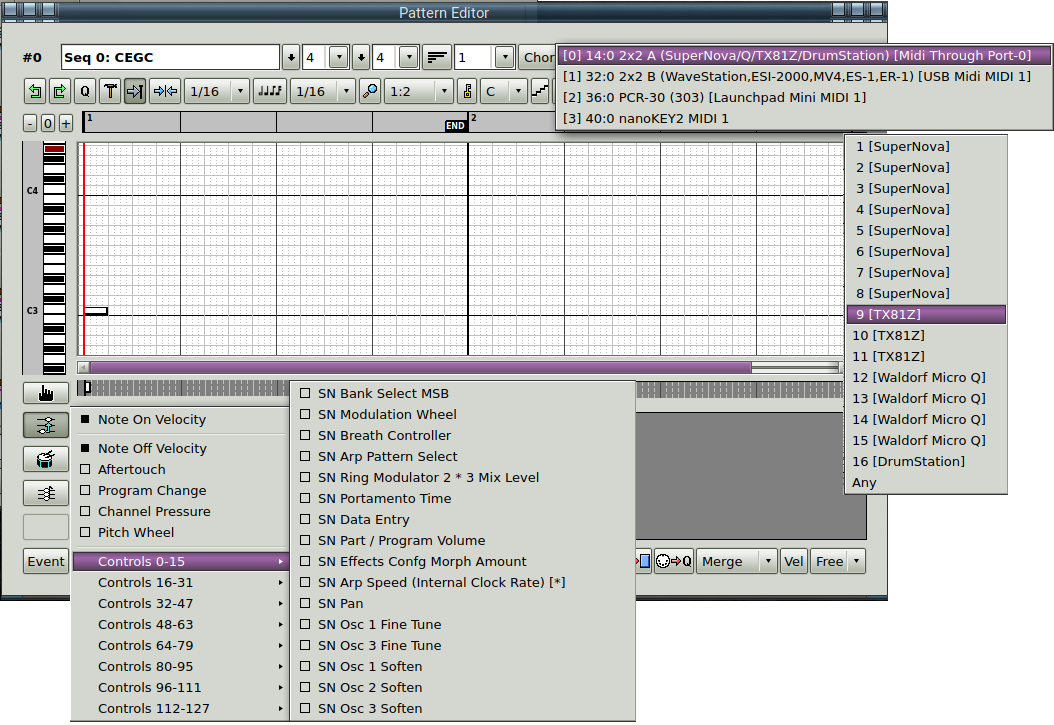
\includegraphics[scale=0.65]{configuration/usr/sample-usr-event-bus-channel-menus.png}
   \caption{Seq66 Composite View of Devices As Set in "sample.usr"}
   \label{fig:sample_usr_event_bus_channel_menus}
\end{figure}

\subsubsection{'usr' File / User Interface Settings}
\label{subsubsec:usr_file_user_interface_settings}

   \index{usr!user-interface-settings}
   \index{[user-interface-settings]}
   \index{usr!interface settings}
   This section, new to \textsl{Seq66}, begins with an
   "INI" group marker \texttt{[user-interface-settings]}.

   It provides for a feature we will hopefully be able to complete some day:
   the complete specificition of the appearance of the user-interface.
   There is plenty of room to change the appearance of
   \textsl{Seq66} already.
   Please try the settings and see what looks good.
   Refer to either the sample file or the file generated when \textsl{Seq66}
   first runs.

   \index{variset}
   \begin{verbatim}
      [user-interface-settings]
      swap-coordinates = false
      mainwnd-rows = 4
      mainwnd-columns = 8
      mainwnd-spacing = 2
      default-zoom = 2
      global-seq-feature = true
      progress-bar-thick = true
      follow-progress = true
      inverse-colors = false
      time-fg-color = "lime"        # same as "default"
      time-bg-color = "black"       # same as "default"
      window-redraw-rate = 40
      window-scale = 1
      window-scale-y = 1
      enable-learn-confirmation = true
   \end{verbatim}

   \texttt{swap-coordinates} allows for an alternate mapping of pattern
   numbers.  (Later, it will also apply to mappings for set-numbers and
   mute-group numbers.)  Here is the pattern layout:

   \begin{verbatim}
      [  0 ] [  1 ] [  2 ] [  3 ] [  4 ] [  5 ] [  6 ] [  7 ]
      [  8 ] [  9 ] [ 10 ] [ 11 ] [ 12 ] [ 13 ] [ 14 ] [ 15 ]
      [ 16 ] [ 17 ] [ 18 ] [ 19 ] [ 20 ] [ 21 ] [ 22 ] [ 23 ]
      [ 24 ] [ 25 ] [ 26 ] [ 27 ] [ 28 ] [ 29 ] [ 30 ] [ 31 ]
   \end{verbatim}

   Compare it to the layout shown in
   \sectionref{paragraph:patterns_pattern_keys}.
   Note that \texttt{progress-bar-thick}also applies to the following:

   \begin{enumerate}
      \item The vertical play-head in the pattern slots.
      \item The vertical play-head in the pattern editor.
      \item The vertical play-head in the song editor.
      \item The font in the pattern slots (Live grid buttons)
         is made bold and made larger when this option is active.
   \end{enumerate}

   There are a number of additional user-interface options.  See the generated
   or sample 'usr' file for descriptions.  Also see the chapter on palettes.

\subsubsection{'usr' File / User MIDI PPQN}
\label{subsubsec:usr_file_user_midi_ppqn}

   The long-standing PPQN for \textsl{Seq24} was a value of 192, and
   \textsl{Seq66} sticks with that default.
   This value is good for most tunes. But other sequencers allow for higher
   values. \textsl{Seq66} allows for some crazy values, ranging from
   32 to 19200.  If a MIDI file has a different PPQN, it will be rescaled to
   the default PPQN.  However, one might want to stick with the PPQN
   specified in the MIDI file, so \textsl{Seq66} allows that as well.
   It is probably best to set \texttt{use-file-ppqn = true}, but that is
   up to the user.

   \index{usr!midi-ppqn}
   \index{default PPQN}
   \index{file PPQN}
   \begin{verbatim}
      [user-midi-ppqn]
      default-ppqn = 192
      use-file-ppqn = true
   \end{verbatim}

\subsubsection{'usr' File / User Randomization}
\label{subsubsec:usr_file_user_randomization}

   The \textbf{Jitter} and \textbf{Randomize} commands available in
   the \textbf{Tools} menu in the pattern editor depend on
   two configurable values.

   \index{usr!midi-ppqn}
   \index{default PPQN}
   \index{file PPQN}
   \begin{verbatim}
      [user-randomization]
      jitter-divisor = 8
      amplitude = 8
   \end{verbatim}

   The \texttt{jitter-divisor} value is used to limit the amount of time
   jitter in jittering note events.  If \texttt{J} is the jitter divisor, than
   the maximum range of time randomization R is: \texttt{R = S / J}, where
   \texttt{S} is the current value of note snap in the pattern editor.
   Thus, the time can be varied by an amount from minus R to plus R.

   The \texttt{amplitude} value is the maximum range (plus or minus) by which
   to modify amplitude values such as note velocity or channel pressure.
   Keep this value small, as the numbers it affects range only from
   0 to 127.

   One minor bug persists in randomization.  As the randomization is applied
   repeatedly, the amplitude tends toward zero.

\subsubsection{'usr' File / User MIDI Settings}
\label{subsubsec:usr_file_user_midi_settings}

   \index{[user-midi-settings]}
   This section begins with an
   "INI" group marker \texttt{[user-midi-settings]}.
   It allows one to specify the
   global defaults for tempo, beats per measure, and so on.

   \index{usr!convert-to-smf-1}
   \index{usr!beats-per-bar}
   \index{usr!beats-per-minute}
   \index{usr!beat-width}
   \index{usr!buss-override}
   \index{usr!velocity-override}
   \index{usr!bpm-precision}
   \index{usr!bpm-step-increment}
   \index{usr!bpm-page-increment}
   \index{usr!bpm-minimum}
   \index{usr!bpm-maximum}
   \begin{verbatim}
      [user-midi-settings]
      convert-to-smf-1 = true
      beats-per-bar = 4
      beats-per-minute = 120
      beat-width = 4
      buss-override = -1
      velocity-override = 80     # velocity_override (-1 = 'Free')
      bpm-precision = 1          # 0, 1, or 2
      bpm-step-increment = 0.1
      bpm-page-increment = 5.0
      bpm-minimum = 0
      bpm-maximum = 127
   \end{verbatim}

   The \texttt{convert-to-smf-1} option is normally true. This causes
   \textsl{Seq66} to convert single track MIDI files (in SMF 0 format) to
   multi-track SMF 1 files.

   \index{port!override}
   \index{buss!override}
   The \texttt{buss-override} option causes the buss-value (port number) to be
   applied to each pattern in a MIDI song that is loaded.  This allows the tune
   to be directed to one's favorite synthesizer/application.
   Unlike the global port override in the main window
   (see \sectionref{subsubsec:introduction_sets_buss_override}),
   this application does not modify the file, though one can still opt to save
   it, which locks in the new buss number.

   The \texttt{velocity-override} option fixes a long standing (from
   \textsl{Seq24}) bug where the actual incoming note velocity was always
   replaced by a hard-wired value.  A value of "-1" corresponds to the "Free"
   setting, which preserves the incoming velocity.

   The \texttt{bpm-precision}, \texttt{bpm-step-increment}, and
   \texttt{bpm-page-increment} values allow more precise control over tempo,
   which makes it easier to match the tempo of external music sources.  Note
   that the step-increment is used by the up/down arrow buttons, the up/down
   arrow keys, and the MIDI BPM control values.  The page-increment is used
   if the BPM field has focus and the Page-Up/Page-Down keys are pressed,
   and new MIDI control values have been added to support coarse MIDI
   control of tempo.

   The \texttt{bpm-minimum} and \texttt{bpm-maximum} settings
   are used in scaling the display of Tempo events.
   By adjusting these values, one can more easily see the variations in
   tempo.  In a main window pattern slot, or in the song editor tempo track,
   this range is scaled to the full range of note values, 0 to 127.
   Generally, one wants to select a range that keeps the main tempo line at
   the middle height of the pattern display.

   To obtain these new settings, remember to backup the existing
   \textsl{seq66.usr}, then run \textsl{Seq66} with the
   \texttt{-{}-user-save} option, and then do a "diff" on the new file and the
   original to merge any old values that need to be preserved.  Then make any
   further tweaks to the new values.

\subsubsection{'usr' File / User Options}
\label{subsubsec:usr_file_user_options}

   \index{[user-options]}
   This section begins with an
   "INI" group marker \texttt{[user-options]}.
   It provides for additional options keyed by the
   \texttt{-o}/\texttt{-{}-option} options.
   This group of options serves to expand the options that are available, since
   \textsl{Seq66} is running out of single-character options.
   This group of options are shown below.

   \index{usr!option-daemonize}
   \index{usr!option-logfile}
   \index{usr!option-pdf-viewer}
   \index{usr!option-browser}
   \begin{verbatim}
      [user-options]
      daemonize = false
      log = "seq66.log"
      pdf-viewer = "/usr/bin/zathura"
      browser = "/usr/bin/lynx"
   \end{verbatim}

   If this option is not used when running \texttt{seq66cli}, then the
   application stays in the console window and dumps informational output to
   it.  If this option is in force, then the only way to affect
   \texttt{seq66cli} is to send a signal (e.g. SIGKILL) to it, or use
   MIDI control.
   However, currently we have issue with this option, so one should run
   \texttt{seq66cli} in the background from a console or from a desktop shortcut.

   The log-file, if specified, is written to the same directory as the 'usr'
   file, the \textsl{Seq66} configuration directory.
   If empty, then a valid file-name can be specified
   in the \texttt{-{}-option log=filename.log} option.
%  There's more to the 'usr' configuration file than we've exposed here.

   The PDF viewer and browser options are used if non-empty.
   Otherwise, the system default applications are used.

\subsubsection{'usr' File / Additional Options}
\label{subsubsec:usr_file_added_options}

   \textbf{\texttt{[user-work-arounds]}} is a section that is a relic from
   older versions of this application.  It can be ignored.  More useful options
   are described below.

\paragraph{'usr' File / Additional Options / [user-ui-tweaks]}
\label{paragraph:user_file_added_options_tweaks}

   \texttt{[user-ui-tweaks]} provides a small number of tweaks to the
   user-interface.

   \begin{verbatim}
      [user-ui-tweaks]
      key-height = 10
      note-resume = false
      style-sheet = "qseq66.qss"    # optional, can include a path
      fingerprint-size = 128
      progress-box-width = 0.8
      progress-box-height = 0.4
      progress-box-shown = true
      progress-note-min = 20
      progress-note-max = 100
      lock-main-window = true
   \end{verbatim}

   \index{key height}
   The \texttt{key-height} option
   affects the default "width" of the piano keys in the pattern
   sequence editor.  Defaults to 12 (pixels).
   This option is also editable in the \textbf{Preferences} dialog.
   There are vertical zoom buttons, and the \texttt{v/0/V} keystrokes to change
   this on the fly, but those changes are not saved.

   \index{new seqedit}
   \textsl{Seq66} can present the pattern editor in the 'Edit' tab
   versus an external window..
   When used in the \textbf{Edit} tab instead of an external window,
   it is shrunk slight vertically to fit controls in the smaller window.

   The following options adopt the new convention for setting variables, in
   which the format is \texttt{item-name = value}.

   \index{note resume}
   The \texttt{note-resume} option, if active, causes any notes in progress
   to be resumed when the pattern is toggled back on.

   \index{style sheet}
   The \texttt{style-sheet} option, if non-empty, causes a user-designed
   style-sheet to be applied.  This is useful in expanding the tab-sizes,
   or making disabled text easier to read in some Qt themes.
   See \texttt{data/samples/textfix.qss} for an example.
   The style sheet file is assumed to reside in the normal \textsl{Seq66}
   configuration directory.
   However, it can have a path component so that the same style sheet
   can be used by many applications more readily.
   Here is an example using the style sheet file
   \texttt{data/samples/qseq66.qss}:

\begin{figure}[H]
   \centering 
   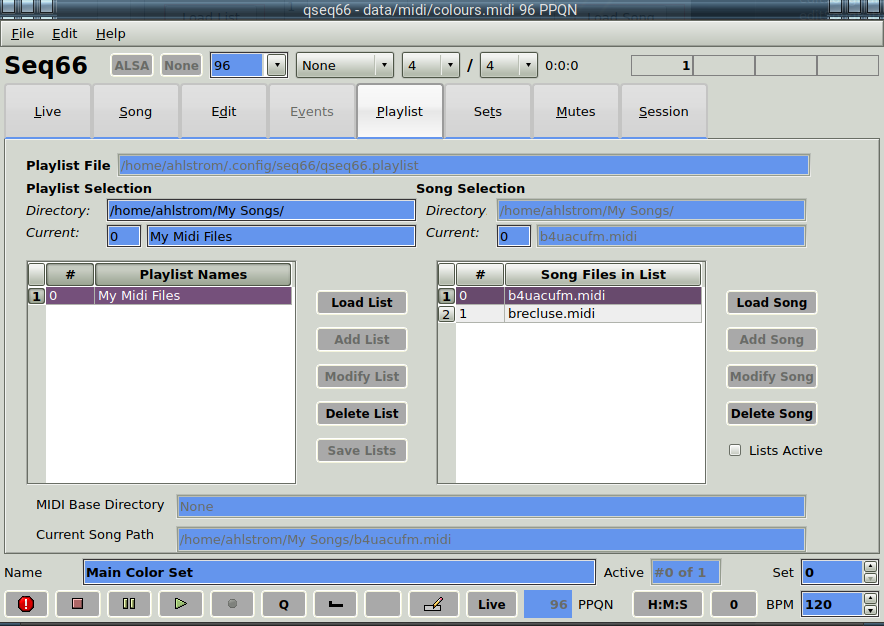
\includegraphics[scale=0.75]{main-window/main-window-stylesheet.png}
   \caption{Seq66 View with Style-Sheet Applied}
   \label{fig:view_with_style_sheet_applied}
\end{figure}

   Note the blue text fields. Also note the larger tabs, which could be useful
   on a touch-screen.
   There is a full-scale dark theme stored in
   \texttt{data/win/dark-theme.qss}.
   One might want to save and tweak the 'palette' file to match.

   The following is a more comprehensive example using
   the \texttt{incrypt-66.qss} style-sheet to control
   the appearance of \textsl{Qt}-drawn items, plus
   the \texttt{incrypt-66.palette} file to alter the colors
   of the drawn elements (grids and live/song backgrounds)
   that are not subject to style-sheet alterations.

\begin{figure}[H]
   \centering 
   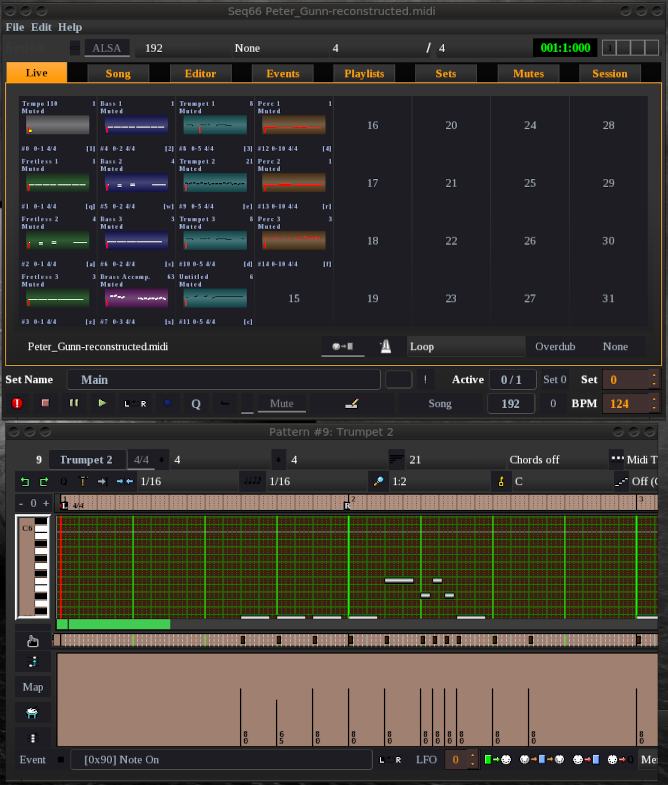
\includegraphics[scale=0.50]{misc/incrypt-66.png}
   \caption{Enhanced "Incrypt" Style-Sheet}
   \label{fig:view_with_enhanced_incrypt_style_sheet}
\end{figure}

   The following shows the \textbf{Song} tab and a sample
   \textbf{Preferences} tab using the same style-sheet and palette.

\begin{figure}[H]
   \centering 
   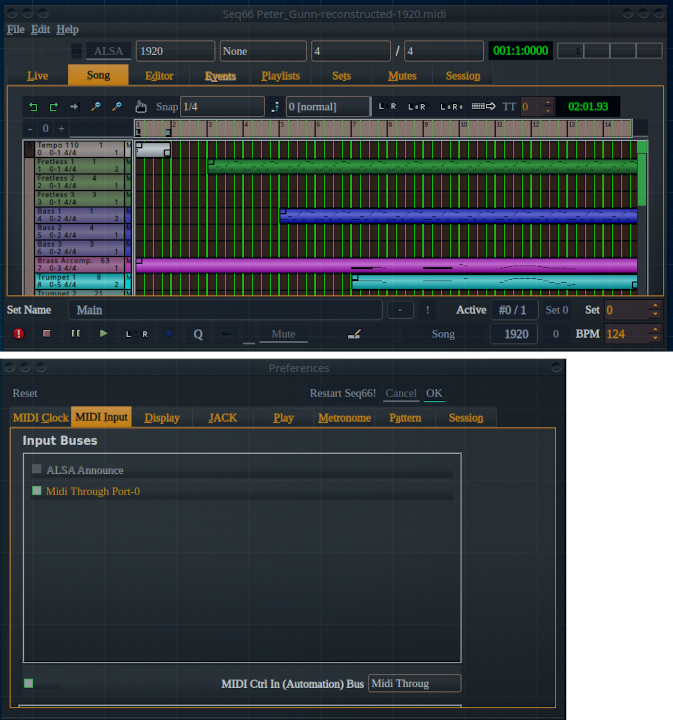
\includegraphics[scale=0.50]{misc/incrypt-66-2.png}
   \caption{Enhanced "Incrypt" Style-Sheet Part 2}
   \label{fig:view_with_enhanced_incrypt_style_sheet_2}
\end{figure}

   The thing to note here is that we must limit the width of combo-boxes so
   that all elements in a horizontal bar can be seen.
   This has the unfortunate side-effect of showing only part of long
   port names (e.g. "Midi Thoug" in the figure above).

   Another interesting style-sheet in \texttt{data/samples} is
   \texttt{perstfix-66.qss}, which is a nice blue theme.
   No need to show it here; try it.

   \index{fingerprint}
   The \texttt{fingerprint} option provides a way to reduce the amount of
   drawing in the pattern grid.  The pattern box in each button is small, and,
   for patterns longer than the fingerprint size, it makes no sense to draw
   hundreds of notes.  Instead, patterns shorter than the fingerprint size are
   drawn normally, while longer patterns are drawn with a "fingerprint", a
   compressed representation of the pattern.

   \index{progress box!width}
   \index{progress box!height}
   The \texttt{progress-box-width} and
   The \texttt{progress-box-height} options provide a way to expand or reduce
   the size of the progess box in each grid button.
   It is purely a user preference.
   The width ranges from 0.5 to 1.0 (full size), with a default of 0.8.
   The height ranges from 0.1 to 1.0 (full size), with a default 0f 0.3.
   Try setting both the width and height to 0.9 for an interesting effect.

%  If either is 0, then the box isn't drawn, and the pattern appears directly
%  on the button.

   \index{progress box!shown}
   If  \texttt{progress-box-shown} is false, then the progress boxes are not
   drawn, and the pattern appears directly on the button.

   \index{progress-note-min}
   \index{progress!note-min}
   \index{progress-note-max}
   \index{progress!note-max}
   The \texttt{progress-note-min} and
   The \texttt{progress-note-max} options change the note range in the progress
   box to control where in "pitch" the notes are shown.

   \index{lock-main-window}
   The \texttt{lock-main-window} option, if true, prevents the main window from
   being resized.  It can still be moved, and the external pattern and song
   editors can still be resized.

\paragraph{'usr' File / Additional Options / [user-session]}
\label{paragraph:user_file_added_options_session}

   \texttt{[user-session]} provides a way to cooperate with the
   \textsl{Non Session Manager}.
   See \sectionref{subsec:sessions_nsm_before_using_nsm}; it goes into great
   detail.

   \begin{verbatim}
      [user-session]
      session = none
      url = ""
   \end{verbatim}

\paragraph{'usr' File / Additional Options / [new-pattern-editor]}
\label{paragraph:user_file_added_options_pattern_editor}

   \texttt{[new-pattern-editor]} contains settings values for recording
    when a new pattern editor is opened. A new pattern is indicated when
   the loop has the default name, \textsl{Unititled}.
    These values save time during a live recording session.
   The valid values for record-style are \texttt{merge},
    \texttt{overwrite}, and \texttt{expand}.

   \begin{verbatim}
      [new-pattern-editor]
      escape-pattern = false
      armed = false
      thru = false
      record = false
      qrecord = false
      record-style = merge
      wrap-around = false
   \end{verbatim}

   The \texttt{escape-pattern} option applies to an open pattern window.
   If enabled, the \texttt{Esc} key can close the pattern window if
   patterns are not playing and if not in paint mode.  If both are true, then
   the first \texttt{Esc} stops playing, the second \texttt{Esc} exits
   paint mode, and the third \texttt{Esc} closes the window.
   The use must enable this option deliberately.

   Also included is a flag to allow notes to wrap around, where the Note On
   comes near the end of the pattern, but the Note Off appears before the
   Note On.
   In this case the end of the note is colored magenta.
   If wrap-around is false, then the note is clipped to the end of the pattern.
   \textbf{Warning}:
   If a song with wrapped notes is re-opened after wrap-around is changed
   to false, then the wrapped notes will be truncated.
%  If false, then two unlinked note events appear in the piano roll, colored
%  magenta.
%  The "u" command in the piano roll will remove them.
   If one does not want to deal with wrap-around at all, then set the pattern
   length to the desired measure count \textsl{plus one} while recording, until
   satisfied with the recording.  Shrink or delete any notes that bleed into
   the extra measure. Then set the pattern back to the desired length.

\subsection{'ctrl' File}
\label{subsec:configuration_ctrl}

   \textsl{Seq66} provides a way to control the
   application to some extent via a MIDI controller, such as a MIDI keyboard or
   a MIDI pad.  The current section describes this feature;
   additional resources and ideas can be found at \url{linuxaudio.org}
   \cite{midicontrol}.
   Also see the tutorial section \sectionref{sec:launchpad_mini}.
   An \textsl{Open Document Format} spreadsheet in the
   \texttt{doc} directory shows layouts for the default
   keystroke configuration (including pattern, mutes, and automation controls)
   and for a couple of \textsl{Launchpad Mini} configurations.
   Another spreadsheet lists the support names for keys; these names can be used
   in the 'ctrl' file, and include some changes for French AZERTY keyboards.
   The spreadsheets are
   \texttt{control\_keys.ods} and
   \texttt{launchpad-mini.ods}.

   The 'ctrl' file provides settings for keyboard control, MIDI control, and
   for specifying MIDI output to reflect \textsl{automation} commands in a
   device such as the \textsl{LaunchPad Mini}.  The name of this file and its
   active status are specfied in the 'rc' file as noted earlier.

\subsubsection{'ctrl' File / MIDI Control Settings}
\label{subsubsec:configuration_ctrl_midi_control_settings}

   \begin{verbatim}
      /home/user/.config/seq66/qseq66.usr             (Linux)
      C:/Users/user/AppData/Local/seq66/qpseq66.usr   (Windows)
   \end{verbatim}

   This file offloads the control settings from the 'rc' file, for a more
   flexible setup. It starts with the sections common to all \textsl{Seq66}
   configuration files.  The first unique section defines some useful settings
   using the new variables feature of the configuration.  Look at the sample or
   generated file to see the layout of these items.

   \begin{verbatim}
      [midi-control-settings]
      control-buss = 3              # or 0xff
      midi-enabled = true
      button-offset = 0
      button-rows = 4
      button-columns = 8
      keyboard-layout = qwerty
   \end{verbatim}

   \begin{itemize}
      \item \texttt{control-buss}.
         The control-buss value ranges from 0 to the maximum buss provided by
         the hardware on the system. If set, then only that buss will be allowed
         to send MIDI control.  A value of 255 or 0xff means any buss can send
         MIDI control. If port-mapping is enabled, the short name (nick-name) of
         the port can be used.
      \item \texttt{midi-enabled}.
         If set to "true", then the MIDI controls will be used.
         It can be set to "false", while keeping the configuration in place
         for later usage.
      \item \texttt{button-offset}.
         This item provides a way to move a set of input controls (e.g. from a
         \textsl{Launchpad Mini}) to a different area of the input control
         device.  Not yet supported.
      \item \texttt{button-rows}.
         Indicates the rows of the input control grid.
         Still in progress.
      \item \texttt{button-columns}.
         Indicates the columns of the input control grid.
         Still in progress.
      \item \texttt{keyboard-layout}.
         Provides a way to adapt to non-US keyboards.
         Currently, the only supported values are "normal" ("qwerty"), "qwertzy",
         and "azerty".
         \index{keys!AZERTY}
         For "azerty", the auto-shift feature of group-learning is disabled.
         The handling of keyboards can be quite complex, and differ between
         Linux distros and Windows.
         Especially problematic are the "dead keys" supported by some locales.
   \end{itemize}

\subsubsection{'ctrl' File / Loop Control}
\label{subsubsec:configuration_ctrl_loop_control}

   The loop-control group consists of 32 lines (0 to 31), one for each
   pattern slot shown in the patterns panel.
   It provides a way to control the arming/disarming (muting/unmuting) of
   each pattern shown in the patterns panel.
   It consolidates the keyboard and MIDI control settings into one table.

   Note that the main window shows the \textsl{active} screen-set.
   These MIDI controls affect the \textsl{active} screen-set.

   This block of matrix elements, numbered from 0 to 31,
   represent control functions (toggle, mute, unmute) for the 32 patterns
   of the active screen-set.
   These 32 rows correspond to the hot-keys assigned in
   the \textbf{File / Options / Keyboard / Control keys [keyboard-group]} 
   configuration panel.

   \index{[loop-control]}
   The MIDI control section begins with the following "INI"-style
   group marker tag, followed by one stanza-line per loop:

   \begin{verbatim}
      [loop-control]
      # Control:  Toggle          On               Off
       0 "1"     [ 0 0x00 0 0 0 ] [ 0 0x00 0 0 0 ] [ 0 0x00 0 0 0 ] # Loop 0
       1 "q"     [ 0 0x00 0 0 0 ] [ 0 0x00 0 0 0 ] [ 0 0x00 0 0 0 ] # Loop 1
       . . .
      31 ","     [ 0 0x00 0 0 0 ] [ 0 0x00 0 0 0 ] [ 0 0x00 0 0 0 ] # Loop 31
   \end{verbatim}

   The first column is an index number, starting at 0.  It indicates what
   loop the control line will affect.
   \index{keys!control}
   The second column is the name of the keystroke that will act as a toggle or
   action key.
   \index{keys!blank}
   If the key name is \texttt{Blank}, then there is no keystroke for that
   pattern control.  The user can specify multiple blank keys as desired.

   The numbers in the leftmost brackets define a \textsl{Toggle} control;
   the numbers in the middle brackets define an \textsl{On} control;
   the numbers in the rightmost brackets define an \textsl{Off} control.
   The numbers inside each set of brackets define six values that set up the
   control.  The layout of each filter inside the brackets is as follows:

      \textbf{[INV STAT D1 D2min D2max]}

   \begin{itemize}
      \item \textbf{INV} = \textbf{inverse}
      \item \textbf{STAT} = \textbf{MIDI status byte} (channel included) 
      \item \textbf{D1} = \textbf{data1}
      \item \textbf{D2min} = \textbf{data2 min}
      \item \textbf{D2max} = \textbf{data2 max}
   \end{itemize}

   If \textbf{STAT} is not 0x00, the control is enabled.  \textsl{Seq66} will
   match the incoming MIDI event against the \textbf{STAT (MIDI status byte)}
   pattern (e.g. a Note On event), and perform the action (On/Off/Toggle) if
   the \textbf{D1} (e.g. a Note number), matches the incoming data, and the
   incoming parameters (e.g. Note velocity) falls in the specified
   \textbf{D2min} to \textbf{D2max} range.  All data values are best specified
   in decimal.

   The \textbf{INV (inverse)} field will make the pattern perform the opposite
   action (\textsl{off} for \textsl{on}, \textsl{on} for \textsl{off}) if the
   data falls outside the specified range.  This is cool because one can map
   several sequences to a knob or fader.

   The \textbf{STAT (MIDI status byte)} field is a MIDI status byte number in
   decimal or hexadecimal notation.
   Remember that it can include a channel.  This channel is not overridden by
   the pattern's selected channel when a MIDI control matching event is
   received. 
%  The channel nybble of this byte is ignored.
   One can look up the possible status values up in the MIDI messages tables;
   the relevant data can be found at \cite{midicontroltable}.
%  As the channel on which the events are sent is ignored,
%  it is sufficient to use the values for channel 1; that is, 0.

   The last three fields describe the range of data that will match.  The
   \textbf{D1 (data1)} field provides the actual MIDI event message number to
   detect, in decimal.  This item could be a Note On/Off event or a
   Control/Mode change event, for example.
   The \textbf{D2min (data2 min)} field is the minimum value of the event for
   the filter to match. For Note On/Off events, this would be the velocity
   value, for example.
   The \textbf{D2max (data2 max)} field is the maximum value of the event for
   the filter to match.

%  This set of values is explained below.

   For each pattern, we can set up MIDI events to turn a 
   pattern on, off, or to toggle it.
   The loop MIDI control setup resembles a matrix.  The default matrix
   uses the central keys on the keyboard, laid out in a 4 x 8 grid matching the
   pattern buttons:

   \begin{verbatim}
      1 2 3 4 5 6 7 8
      q w e r t y u i
      a s d f g h j k
      z x c v b n m <
   \end{verbatim}

   Please note that the buttons on some (or most) MIDI controllers send a
   message on press and another message on release.  One can set such buttons
   up as toggle buttons by defining only the "Toggle" (first) stanza.
   Or one can have the button active the function on press, and then deactivate
   it on release by defining the "On" (second) and "Off" (third) stanzas
   appropriately.

\subsubsection{'ctrl' File / Mute-Group Control}
\label{subsubsec:configuration_ctrl_mute_group_control}

   \index{mute-group control}
   This section provides controls for 32 groups of mutes.
   A group is a set of patterns that can toggle their playing state
   together.  Every group contains all 32 sequences in the active screen set.
   So, this part of the MIDI Control section is used for muting and unmuting
   (and toggling) a group of patterns using a keystroke or MIDI control.
   The definitions are in the same format as the loop-control section.

   \begin{verbatim}
      [mute-group-control]
        0 "!"  [ 0 0x00 0 0 0 ] [ 0 0x00 0 0 0 ] [ 0 0x00 0 0 0 ] # Mute 0
        1 "Q"  [ 0 0x00 0 0 0 ] [ 0 0x00 0 0 0 ] [ 0 0x00 0 0 0 ] # Mute 1
       . . .
       31 "<" [ 0 0x00 0 0 0 ] [ 0 0x00 0 0 0 ] [ 0 0x00 0 0 0 ]  # Mute 31
   \end{verbatim}

   All this section does is set up the controls to be used; the actual
   mute-group patterns are defined in the 'mutes' configuration file (or in the
   \textsl{Seq66} MIDI file itself.
   A key name of \texttt{Blank} can be used to disable a keystroke for
   that line.

   The mutes MIDI control setup resembles a matrix match the shifted versions
   of the loop control keys.  The default matrix
   uses the central keys on the keyboard, laid out in a 4 x 8 grid matching the
   pattern buttons:

   \begin{verbatim}
      ! @ # $ % ^ & *
      Q W E R T Y U I
      A S D F G H J K
      Z X C V B N M <
   \end{verbatim}

\subsubsection{'ctrl' File / Automation Control}
\label{subsubsec:configuration_midi_ctrl_automation}

   This section provides ways to control \textsl{Seq66} push-button controls
   from a keyboard or from a MIDI device.
   These entries control
   \textsl{Seq66} actions like changing the BPM value, screen-set,
   record, solo, etc.

   Note that automation controls that depend upon a parameter (such as group
   number or loop number) can only work with a MIDI control.
   MIDI control can provide parameters via a control value, note number or value,
   etc.
   Key control can provide only a "press" or "release" status.
   
   Each item in this group consists of one line.  Each line
   specifies a MIDI event that can cause a given
   \textsl{Seq66} user-interface operation to occur.
   These items are easy to view in the 'ctrl' configuration file,
   in the \texttt{[automation-control]} section.

   \begin{verbatim}
      [automation-control]
       0 "'"    [ 0 0x00 0 0 0 ] [ 0 0x00 0 0 0 ] [ 0 0x00 0 0 0 ] # BPM Up
       1 ";"    [ 0 0x00 0 0 0 ] [ 0 0x00 0 0 0 ] [ 0 0x00 0 0 0 ] # BPM Dn
       . . .
      35 "Quit" [ 0 0x00 0 0 0 ] [ 0 0x00 0 0 0 ] [ 0 0x00 0 0 0 ] # Loop 0
       . . .
      48 "0xfe" [ 0 0x00 0 0 0 ] [ 0 0x00 0 0 0 ] [ 0 0x00 0 0 0 ] # Reserved 48
       . . .
      80 "0x8f" [ 0 0x00 0 0 0 ] [ 0 0x00 0 0 0 ] [ 0 0x00 0 0 0 ] # All Sets
   \end{verbatim}

   One thing to be careful of when editing this section is to make
   all the numbers (from 0 to 80) unique. When copy/pasting a line and
   forgetting to change the number (\textsl{mea culpa}),
   an error like the following can appear in the console output:

   \begin{verbatim}
      Duplicate mute slot # 43 : '0xe8'
      [seq66] Key controls: Error at line 232 ordinal 0xe8 key
         '0xe8' control 'Visibility' code 43
   \end{verbatim}

   Note that "Quit" is not a real keystroke.  It is a placeholder in the
   internal keystroke map for the functionality of quitting \textsl{Seq66} via
   MIDI control.  Qt provides other ways to quit via keystroke.  A key name of
   \texttt{Blank} can be used to disable a keystroke for a line.  The stanzas
   meaning can change depending on the type of control.  Here are
   the important styles:

   \begin{verbatim}
      Normal:        [ Toggle       ] [ On          ] [ Off             ]
      Playback:      [ Pause Play   ] [ Start Play  ] [ Stop Play       ]
      Play list:     [ Select by D2 ] [ Select Next ] [ Select Previous ]
      Play song:     [ Select by D2 ] [ Select Next ] [ Select Previous ]
   \end{verbatim}

   For selecting play-lists and songs by number, \textbf{D2} is used.
   Thus, one possible value to use to select would be to use a 
   Note On event on channel 16 (0x9F) with a note number of 0 (a rarely-used
   note in any tune), and list/song numbers ranging from 0 to 127.  Using note
   0 for list selection and note 1 for song selection:

   \begin{verbatim}
      24 "F2" [ 0 0x9F   0   0 127 ] [ . . . ] [ . . .] # Play List
      25 "F3" [ 0 0x9F   1   0 127 ] [ . . . ] [ . . .] # Play Song
   \end{verbatim}

   Obviously, this requires a MIDI controller for which the velocity can be
   exactly specified.  One can also reserve \textbf{D2} values of 126 for
   "previous" and 127 for "next".

\paragraph{Automation / BPM Up and Down}
\label{paragraph:configuration_midi_ctrl_bpmupdn}

   These controls increment or decrement the beats-per-minute setting, as if
   the up- or down-arrow has been clicked in the BPM combox-box, or the up- or
   down-arrow key pressed, in that combo-box.
   This increment is the
   \index{bpm!step increment}
   \index{usr!step increment}
   "step increment" which defaults to 1, but can be modified by
   changing the "bpm\_step\_increment" value in the 'usr'
   configuration file.

\paragraph{Automation / Screen-Set Up and Down}
\label{paragraph:configuration_midi_ctrl_ssupdn}

   Also abbreviated "Set Up" and "Set Down".
   This control increments / decrements to the next / previous screen-set. 
   Once the screen-set has been altered, mute-groups and other
   actions apply to that screen set.

\paragraph{Automation / Mod Replace}
\label{paragraph:configuration_midi_ctrl_modrep}

   This entry controls the "replace" flag.
   Once set, when the user manually clicks a pattern slot,
   that pattern is unmuted, and all the rest are muted.
   Thus, this MIDI control is kind a of "Solo" function.
   It works whether in "Live" or "Song" mode.

\paragraph{Automation / Mod Snaphot}
\label{paragraph:configuration_midi_ctrl_modsnap}

   This control causes the playing statuses of all active
   (i.e. having data) patterns to be saved.  When turned off, the
   original playing status is restored.
%  Thus, two MIDI events
%  need to be allocated to this functionality.

\paragraph{Automation / Mod Queue}
\label{paragraph:configuration_midi_ctrl_modqueue}

   This control sets up the "queue" status flag.
   Then, when the user manually clicks a pattern slot,
   that pattern is queued, and will play at the next cycle of the
   pattern.

   Here is an example from \cite{midicontrol}, which shows how to set up
   the "Sustain" control-change event to queue or un-queue a sequence:
   The \textsl{Akai MPK Mini} has a Sustain button and we can set the
   Sustain MIDI event (with MIDI status byte 176 [0xB0] to represent a
   Controller event, and control/mode change number 64 [0x40] to
   represent the Sustain or Pedal control) up as the queue modifier in
   the \texttt{mod queue} entry:

   \begin{verbatim}
      6 "o" [ 0  0x00 0  0  0 ] [ 0  0xB0 64 127 127 ] [ 0  0xB0 64 0  0 ]
      #      INV STA  D1 mn mx   INV STA  D1 mn  mx     INV STA D1  mn mx
      #                                   ^  ^                      ^  ^
      #                                   |  |                      |  |
      #                                   |   ----Sustain-----------   |
      #                                    -------Control Change-------
   \end{verbatim}

   So when the Sustain button is held down, and one presses one of the pads
   on the \textsl{MPK Mini}, the corresponding sequence gets queued.
   Also included in the data directory are sample 'ctrl' files for other devices.

\paragraph{Automation / Mute Group ("Group Mute")}
\label{paragraph:configuration_midi_ctrl_modgmute}

   To be documented.

\paragraph{Automation / Group Learn}
\label{paragraph:configuration_midi_ctrl_modglean}

   This MIDI control sets up a "group learn".
   This control sets two internal flags on : "mode-group" and "group-learn".
   The first flag indicates that we will be handling mute-groups.
   The second flag indicates that we are learning these mute-groups,
   effectively recording the current status of all the patterns in all of the
   screen-sets.

   \index{L button}
   Note that this control corresponds to the "L" button in the main window
   user-interface.
   \index{keys!l}
   It can also be accessed by the default hot-key, \texttt{l}.
   Note that, once in learn-mode, there is no way to cancel learn-mode
   except by selecting an illegal mute-group keystroke.
   Also see \sectionref{sec:mutes_master}.

\paragraph{Automation / Playing Set}
\label{paragraph:configuration_playing_set}

   To be documented.

\paragraph{Automation / Playback}
\label{paragraph:configuration_playback}

   This automation entry defaults to a period.
   It starts playback and stops (pauses) playback.
   Note that this applies to the live grid.
   For the pattern and song editor piano rolls, it is hardwired.

\paragraph{Automation / Song Record}
\label{paragraph:configuration_song_record}

   Initiates a "recording" of the musician's muting and unmutings as triggers
   in the song editor.

   There are still some wrinkles to work out with this, such as ignoring snap
   values in order to get an exact recording of the triggers.

\paragraph{Automation / Solo}
\label{paragraph:configuration_midi_ctrl_solo}

   Meant to "solo" a given track.
   Needs testing and further work.

\paragraph{Automation / Theu}
\label{paragraph:configuration_midi_ctrl_thru}

   Turns on the "MIDI Thru" function of the current pattern as displayed in a
   pattern editor.  More testing needed.

\paragraph{Automation / BPM Page Up and Page Down}
\label{paragraph:configuration_midi_ctrl_bpmpageupdn}

   Similar to
   \sectionref{paragraph:configuration_midi_ctrl_bpmupdn}, but in
   larger steps.
   These controls increment or decrement the beats-per-minute setting
   in large steps, as if
   the Page-Up or Page-Down were pressed in the BPM combox-box.
   This increment is the
   \index{bpm!page increment}
   \index{usr!page increment}
   "page increment" which defaults to 10, but can be modified by
   changing the "bpm\_page\_increment" value in the 'usr'
   configuration file.

\paragraph{Automation / Set a Set}
\label{paragraph:configuration_midi_set_a_set}

   Changes to a set as given by the data parameter.
   Needs more testing and further work.

% \paragraph{Automation / Screen-Set Play}
% \label{paragraph:configuration_midi_ctrl_ssplay}

%  This MIDI control sets the playing screen-set.

\paragraph{Automation / Loop Mode}
\label{paragraph:configuration_midi_loop_mode}

   Toggles using the "L/R" markers as the beginning and ending
   of playback.

   See \sectionref{paragraph:configuration_bbthms_lr_loop}.

\paragraph{Automation / Quan Record}
\label{paragraph:configuration_midi_quanrecord}

   Toggles quantization of the incoming note events while recording.

\paragraph{Automation / Reset Sets}
\label{paragraph:configuration_midi_reset_sets}

   Resets the set counter to set 0.

\paragraph{Automation / One-shot}
\label{paragraph:configuration_midi_one_shot}

   Toggles one-shot recording mode.

\paragraph{Automation / FF, Rewind, and Top}
\label{paragraph:configuration_midi_ff_rewind_top}

   When activated, each command moves the playing tick value up or down
   by one-half of a measure.
   The "Top" command rewinds to the beginning immediately.

\paragraph{Automation / Playlist Commands}
\label{paragraph:configuration_midi_playlist_commands}

   The "Play List" and "Play Song" automation commands allow one
   to select a particular play-list or song,
   or increment/decrement to the next/previous one.

\paragraph{Automation / Tap BPM}
\label{paragraph:configuration_midi_tap_bpm}

   This command, when pressed repeatedly, sets the beats-per-minute
   value to the interval between the taps.

\paragraph{Automation / Start}
\label{paragraph:configuration_start}

   This automation entry defaults to a space.
   It starts playback and stops playback with a rewind to the beginning.
   Note that this applies to the live grid.
   For the pattern and song editor piano rolls, it is hardwired.

\paragraph{Automation / Stop}
\label{paragraph:configuration_stop}

   This automation entry defaults to an escape character.
   It stops playback with a rewind to the beginning.
   Note that this applies to the live grid.
   For the pattern and song editor piano rolls, it is hardwired,
   and this keystroke can be used to exit insert/paint mode.

\paragraph{Automation / Toggle Mute}
\label{paragraph:configuration_toggle_mute}

   Reverses the armed statuses of the current set.

\paragraph{Automation / Song Position}
\label{paragraph:configuration_song_position}

   This one needs work. We can't even remember what it means!

\paragraph{Automation / Keep Queuue}
\label{paragraph:configuration_keep_queue}

   When given, this command turns on keep-queue mode.

\paragraph{Automation / Slot Shift}
\label{paragraph:configuration_slot_shift}

   When given, this command allows for accessing patterns numbered
   from 32 to 63.
   When given again, this command allows for accessing patterns numbered
   from 64 to 95.
   Useful only when set sizes of 64 and 96 are configured.

\paragraph{Automation / Record Modes and Quantization}
\label{paragraph:configuration_midi_record_quan}

   For release 0.97.3,
   \index{patterns-panel!modes}
   \index{grid modes}
   \textbf{grid modes} have been introduced.
   The \textbf{Record} and \textbf{Quan Record} automation controls have been
   refactored to cycle through these modes.
   Additional automation commands provide direct access to each mode.

   Grid mode changes the function of the main window's patterns panel so that
   it can be used to initiate record instead of toggling mute status,
   regardless of whether the toggling is done via the buttons, hot-keys, or
   MIDI controls.  The following modes are supported:

   \begin{itemize}
      \item \textbf{Loop}.
         The normal toggling of the mute/armed status of
         a pattern the slot is clicked or activated by its hot-keys.
      \item \textbf{Mutes}.
         Applies the given mute-group statuses when
         the slot is clicked. Since the "shifted" hot-keys can also be used,
         this mode is most useful with mouse-click control.
      \item \textbf{Record}.
         In this mode, a click on a slot or the use of its hot-key toggles
         recording for that pattern.
      \item \textbf{Copy}.
         Copies the pattern when that slot is clicked.
      \item \textbf{Paste}.
         Pastes the previously-copied pattern into the slot
         that is clicked.
      \item \textbf{Clear}.
         Clears the pattern in the clicked slot.
         The pattern remains in that slot, but it has no events.
      \item \textbf{Delete}.
         Deletes the pattern in the clicked slot.
      \item \textbf{Thru}.
         Enables the MIDI Thru function for that pattern.
      \item \textbf{Solo}.
         Solos the clicked pattern.
      \item \textbf{Cut}.
         Deletes the pattern in the clicked slot, while saving it.
      \item \textbf{Double}.
         Doubles the length (in measures) of the pattern in the slot
         that is clicked.
   \end{itemize}

   A click or a hot-key will cause the selected function above to be applied to
   the pattern denoted by the click/key.
%  For details, see \sectionref{paragraph:patterns_recording_modes}.
   In \textbf{Record} mode, the following settings are enabled:

   \begin{itemize}
      \item \textbf{Overdub}.
         Called \textbf{Merge} in the pattern editor, this recording
         style just keeps adding events as they come in when the
         pattern repeats.
      \item \textbf{Overwrite}.
         When the pattern ends, then loops back to the beginning,
         an incoming note clears the pattern before being added.
      \item \textbf{Expand}.
         As notes come in, the pattern gets longer and longer.
      \item \textbf{One-shot}.
         Notes are added to the pattern as they come in, but recording
         stops when the end of the pattern's specified measures is
         reached.
      \item \textbf{One-shot Reset}.
         Similar to one-shot, but clears the pattern.
         (To do: find the exact process used here.)
   \end{itemize}

%  For details, see \sectionref{paragraph:patterns_recording_modes}.
   Also supported is changing the mode of recording, that is, what happens
   to notes while incoming during recording:

   \begin{itemize}
      \item \textbf{No Quan}.
         Nothing is done to the incoming notes.
      \item \textbf{Quantize}.
         Incoming notes are quantized to the nearst snap value for the
         pattern.
      \item \textbf{Tighten}.
         Incoming notes are tightened (partially quantized)
         to the nearst snap value for the pattern.
      \item \textbf{Randomize}.
         The amplitude (velocity) of notes is randomized.
         This is not done during recording, but can be applied later.
      \item \textbf{Jitter}.
         The timing of notes is randomized.
         This is not done during recording, but can be applied later.
      \item \textbf{Note-map}.
         If active, the specified 'drums' file values are used to remap the
         notes to new notes. This is useful, along with setting MIDI Thru, to
         play on a pre-General-MIDI drum machine (e.g. Yamaha DD-11) and
         hear it transmuted to GM while recording. Can also be applied after
         the fact, if the pattern is marked as transposable.
      \end{itemize}

%  For details, see \sectionref{paragraph:patterns_recording_modes}.
   Also see \sectionref{subsec:pattern_editor_bottom} for more information on these
   recording modes.

\paragraph{Automation / BBT/HMS and LR Loop}
\label{paragraph:configuration_bbthms_lr_loop}

   These commands toggle the display of bars:beats:ticks versus
   hours:minutes:seconds, and looping between the L/R markers.

   See \sectionref{paragraph:configuration_midi_loop_mode}.

\paragraph{Automation / Undo and Redo}
\label{paragraph:configuration_undo_redo}

   These commands undo or redo actions such as deleting notes.
   \textbf{Important}:
   These commands will affect \textsl{all} open pattern editors!

\subsubsection{Automation / More MIDI Control}
\label{subsubsec:configuration_midi_ctrl_automationex}

   Many additional control items were requested by users, to control
   additional features of the application.  Too many to list here.
   See the 'ctrl' file samples for more information.
   We will ultimately mention them all.

   Some important ones to touch on:

   \begin{itemize}
      \item \textbf{Visibility}.
         Toggles the visibility of the user-interface.
         This can be useful in some circumstances.
         In addition, the session manager, if in force, might
         issue this command.
      \item \textbf{Quit}.
         Provides a way to exit \textsl{Seq66} via MIDI control.
   \end{itemize}

\subsubsection{'ctrl' File / MIDI Control Output}
\label{subsubsec:configuration_ctrl_midi_control_out}

   This section provides a way to have a MIDI device, such as the
   \textsl{Novation Launchpad Mini}, show the status
   of the patterns that are active, as well as other information.
   The first sub-section sets up some general settings.

   \begin{verbatim}
      [midi-control-out-settings]
      set-size = 32
      output-buss = 1
      midi-enabled = true
      button-offset = 0
      button-rows = 8
      button-columns = 8
   \end{verbatim}

   \begin{itemize}
      \item \texttt{set-size}.
         Provides the set size.  The default is 32, in a 4 x 8 grid.
      \item \texttt{output-buss}.
         Indicates where automation-display controls are to be sent.
         Specify the output buss to which the display device is attached. If
         port-mapping is enabled, the short name (nick-name) of the port can be
         used.
      \item \texttt{midi-enabled}.
         If set to "true", then the MIDI control outputs will be used.
         It can be set to "false", while keeping the configuration in place
         for later usage.
      \item \texttt{button-offset}.
         This item provides a way to move a set of output controls (e.g. from a
         \textsl{Launchpad Mini}) to a different area of the output control
         device.  Not yet supported.
      \item \texttt{button-rows}.
         Indicates the rows of the output control grid.
         Still in progress.
      \item \texttt{button-columns}.
         Indicates the columns of the output control grid.
         Still in progress.
   \end{itemize}

   \begin{verbatim}
      [midi-control-out]
       0 [ 0x90  0 60 ] [ 0x90  0 15 ] [ 0x90  0 62 ] [ 0 0x90  0 12 ]
       1 [ 0x90  1 60 ] [ 0x90  1 15 ] [ 0x90  1 62 ] [ 0 0x90  1 12 ]
      . . .
      31 [ 0x90 31 60 ] [ 0x90 31 15 ] [ 0x90 31 62 ] [ 0 0x90 31 12 ]
   \end{verbatim}

   The first number is the pattern number of the pattern whose armed/muted
   status is to be shown.
   There are samples in the \texttt{data/linux} directory for some devices that
   one can adapt to other equipment.
   The mute-group buttons and their status can also be shown:

   \begin{verbatim}
      [mute-control-out]
       0 [ 0x00   0   0 ] [ 0x00   0   0 ] [ 0x00   0   0 ]
       1 [ 0x00   0   0 ] [ 0x00   0   0 ] [ 0x00   0   0 ]
        . . .
      31 [ 0x00   0   0 ] [ 0x00   0   0 ] [ 0x00   0   0 ]
   \end{verbatim}

   There are additional automation controls whose status can be displayed:

   \begin{verbatim}
      [automation-control-out]
      0 [ 0x00   0   0 ] [ 0x00   0   0 ] [ 0x00   0   0 ]  # Panic
      0 [ 0x00   0   0 ] [ 0x00   0   0 ] [ 0x00   0   0 ]  # Stop
       . . .
      0 [ 0x00   0   0 ] [ 0x00   0   0 ] [ 0x00   0   0 ]  # Tap_BPM
      0 [ 0x00   0   0 ] [ 0x00   0   0 ] [ 0x00   0   0 ]  # Quit
   \end{verbatim}

   See the sample files for more detailed descriptions.
   Also see \sectionref{sec:launchpad_mini}; it showns a fairly comprehensive
   setup based on the file \texttt{data/linux/qseq66-lp-mini.ctrl}.

\subsubsection{'ctrl' File / Macro Control Output}
\label{subsubsec:configuration_ctrl_macro_control_out}

   This section provides a way to send setup information to a MIDI device,
   such as the \textsl{Novation Launchpad Pro Mk3}.
   There is too much involved (especially that device) to discuss in
   detail here, but this feature can be used to put a device into
   "programmer" mode at \textsl{Seq66} startup and back into
   "normal" mode at \textsl{Seq66} shutdown.
   Here is a hypothetical sample for the Mk3:

   \begin{verbatim}
      [macro-control-out]
      footer = 0xf7
      header =0xf0 0x00 0x20 0x29 0x02 0x0e 
      reset = $shutdown
      shutdown = $live-mode
      startup = $programmer-mode
      live-mode = $header 0x0e 0x00 $footer
      programmer-mode = $header 0x0e 0x01 $footer
   \end{verbatim}

   The macros "footer", "header", "reset", "startup", and "shutdown"
   are written to the 'ctrl' file if not already present, though
   they won't have any useful definition.
   The first three are useful in other macros, while "startup" and
   "shutdown", if defined with actual data, are sent at the launch
   and shutdown, respectively, of \textsl{Seq66}.
   Note that these macros can be re-used in other macros, to
   increase the readability of the macros and to reduce the
   chance for mistakes.
   Note, too, that many devices required a device-specific
   SysEx header to precede the command-data, and the 0xf7
   End-of-SysEx "footer" to end the command.

   There is no limit to the number of macros that can be defined.
   To send any of them directly at any time, go to the
   \textbf{Session} tab and select a macro from the drop-down list.

   There is currently no way to send them via MIDI control.

% For editability, the default keys are specified in another TeX file.

%-------------------------------------------------------------------------------
% defaultkeys
%-------------------------------------------------------------------------------
%
% \file        defaultkeys.tex
% \library     Documents
% \author      Chris Ahlstrom
% \date        2021-12-04
% \update      2023-10-25
% \version     $Revision$
% \license     $XPC_GPL_LICENSE$
%
%     Provides the default-keys section of seq66-user-manual.tex.
%
%-------------------------------------------------------------------------------

\subsubsection{'ctrl' File / Keyboard / Default Assignments}
\label{subsubsec:ctrl_keyboard_default_assignments}

   This section provides a table of the functions, key numbers ("ordinals"),
   names, and other information about the default \textsl{Seq66}
   keyboard assignments.
   Also see the installed \texttt{control\_keys.ods} spreadsheet, which
   might be more up-to-date.

   The following status tags apply in this table.
   We're trying to support all keystrokes, but Qt and international keyboards
   make it sometimes difficult.

   \begin{itemize}
      \item \textbf{(X)}.
         Avoid using.  Applies to the modifier keys Alt, Ctrl, Meta, Shift, etc.
         Also applies to tricky internal keys like the grave (backtick).
         One can try them, however, to see what happens.
      \item \textbf{(D)}.
         In the default configuration. Applies especially to the default
         loop-control and mute-group control keys that reside in the main part of
         the keyboard.
      \item \textbf{(d)}.
         In the default configuration, but no functionality yet.
      \item \textbf{(p)}.
         Available as a place-holder (a hex value)
      \item \textbf{(H)}.
         Hard-wired keys like Esc, Space, and the main arrow keys.  Avoid using.
      \item \textbf{(A)}.
         Available for usage.
      \item \textbf{(!)}.
         Needs investigation.
      \item \textbf{(?)}.
         Needs investigation.
      \item \textbf{*}. An asterisk added means "to do", as does the word
         "Reserved".
   \end{itemize}

   Because of the size of the table, and not wanting to deal with \textsl{LaTEX}
   long-table issues, we break the table into sections.
   These tables follow, some of them moved into following pages.
   
   The first section is \tableref{table:key_defaults_ctrl_keys}.
   Because of potential conflicts with user-interface keys, we do
   not recommend configuring them.
   However, we do use some of them for controls
   that are not yet effective. And, go ahead a try them if you want.
   The user rules!

   \begin{table}[htb!]
      \centering
      \caption{Key Defaults. Control Keys}
      \label{table:key_defaults_ctrl_keys}
      \begin{tabular}{l l l l l}
        \textbf{Function} & \textbf{Status} & \textbf{Ordinal} & \textbf{Name} & \textbf{Modifier} \\
        None               & (X)  &  0x00   & "NUL"        & Ctrl \\
        None               & (X)  &  0x01   & "SOH"        & Ctrl \\
        None               & (X)  &  0x02   & "STX"        & Ctrl \\
        None               & (X)  &  0x03   & "ETX"        & Ctrl \\
        None               & (X)  &  0x04   & "EOT"        & Ctrl \\
        None               & (X)  &  0x05   & "ENQ"        & Ctrl \\
        None               & (X)  &  0x06   & "ACK"        & Ctrl \\
        None               & (X)  &  0x07   & "BEL"        & Ctrl \\
        None               & (!)  &  0x08   & "BS"         & Ctrl \\
        None               & (X)  &  0x09   & "HT"         & Ctrl \\
        None               & (!)  &  0x0a   & "LF"         & Ctrl \\
        None               & (X)  &  0x0b   & "VT"         & Ctrl \\
        None               & (X)  &  0x0c   & "FF"         & Ctrl \\
        None               & (X)  &  0x0d   & "CR"         & Ctrl \\
        None               & (X)  &  0x0e   & "SO"         & Ctrl \\
        None               & (X)  &  0x0f   & "SI"         & Ctrl \\
        None               & (X)  &  0x10   & "DLE"        & Ctrl \\
        None               & (X)  &  0x11   & "DC1"        & Ctrl \\
        None               & (X)  &  0x12   & "DC2"        & Ctrl \\
        None               & (X)  &  0x13   & "DC3"        & Ctrl \\
        None               & (X)  &  0x14   & "DC4"        & Ctrl \\
        None               & (X)  &  0x15   & "NAK"        & Ctrl \\
        None               & (X)  &  0x16   & "SYN"        & Ctrl \\
        None               & (X)  &  0x17   & "ETB"        & Ctrl \\
        None               & (X)  &  0x18   & "CAN"        & Ctrl \\
        None               & (X)  &  0x19   & "EM"         & Ctrl \\
        None               & (X)  &  0x1a   & "SUB"        & Ctrl \\
        None               & (X)  &  0x1b   & "ESC"        & Ctrl \\
        None               & (X)  &  0x1c   & "FS"         & Ctrl \\
        None               & (X)  &  0x1d   & "GS"         & Ctrl \\
        None               & (X)  &  0x1e   & "RS"         & Ctrl-Shift \\
        None               & (X)  &  0x1f   & "US"         & Ctrl-Shift \\
      \end{tabular}
   \end{table}

   The next section is \tableref{table:key_defaults_ascii_keys_1}.
   These deal with some of the pattern hot-keys ("Loop")
   and their shifted mute-group ("Mutes") keys.
   We do not show the numbers, as they are logically laid out on the U.S.
   keyboard.
   The Space and Period keys are hardwired ("*")
   for Start/Stop/Pause in the pattern piano roll and the song-editor
   piano roll.

   \begin{table}[htb!]
      \centering
      \caption{Key Defaults. ASCII Keys 1}
      \label{table:key_defaults_ascii_keys_1}
      \begin{tabular}{l l l l l}
        \textbf{Function} & \textbf{Status} & \textbf{Ordinal} & \textbf{Name} & \textbf{Modifier} \\
        Start/Stop *       & (H)  &  0x20   & "Space"      & none \\
        Mutes              & (D)  &  0x21   & "!"          & Shift \\
        None               & (A)  &  0x22   & "\""         & Shift \\
        Mutes              & (D)  &  0x23   & "\#"         & Shift \\
        Mutes              & (D)  &  0x24   & "\$"         & Shift \\
        Mutes              & (D)  &  0x25   & "\%"         & Shift \\
        Mutes              & (D)  &  0x26   & "\&"         & Shift \\
        BPM Up             & (D)  &  0x27   & "'"          & Shift \\
        None               & (A)  &  0x28   & "("          & Shift \\
        None               & (A)  &  0x29   & ")"          & Shift \\
        Mutes              & (D)  &  0x2a   & "*"          & Shift \\
        None               & (A)  &  0x2b   & "+"          & Shift \\
        None               & (D)  &  0x2c   & ","          & none \\
        Event Edit         & (D)  &  0x2d   & "-"          & Set-mode \\
        Play/Pause *       & (H)  &  0x2e   & "."          & none \\
        Slot Shift         & (H)  &  0x2f   & "/"          & none \\
        Clear Mutes        & (D)  &  0x30   & "0"          & none \\
        Loop               & (D)  &  0x31   & "1"          & none \\
        Loop               & (D)  &  0x32   & "2"          & none \\
        Loop               & (D)  &  0x33   & "3"          & none \\
        Loop               & (D)  &  0x34   & "4"          & none \\
        Loop               & (D)  &  0x35   & "5"          & none \\
        Loop               & (D)  &  0x36   & "6"          & none \\
        Loop               & (D)  &  0x37   & "7"          & none \\
        Loop               & (D)  &  0x38   & "8"          & none \\
        None               & (A)  &  0x39   & "9"          & none \\
        None               & (A)  &  0x3a   & ":"          & Shift \\
        BPM Down           & (D)  &  0x3b   & ";"          & none \\
        Loop               & (D)  &  0x3c   & "<"          & Shift \\
        Pattern Edit       & (D)  &  0x3d   & "="          & Set-mode \\
        None               & (A)  &  0x3e   & ">"          & Shift \\
        None               & (A)  &  0x3f   & "?"          & Shift \\
      \end{tabular}
   \end{table}

   The next section is \tableref{table:key_defaults_ascii_keys_2}.
   These deal mainly with the shifted mute-group ("Mutes") keys.

   \begin{table}[htb!]
      \centering
      \caption{Key Defaults. ASCII Keys 2}
      \label{table:key_defaults_ascii_keys_2}
      \begin{tabular}{l l l l l}
        \textbf{Function} & \textbf{Status} & \textbf{Ordinal} & \textbf{Name} & \textbf{Modifier} \\
        Mutes              & (D)  &  0x40   & "@"          & Shift \\
        Mutes              & (D)  &  0x41   & "A"          & Shift \\
        Mutes              & (D)  &  0x42   & "B"          & Shift \\
        Mutes              & (D)  &  0x43   & "C"          & Shift \\
        Mutes              & (D)  &  0x44   & "D"          & Shift \\
        Mutes              & (D)  &  0x45   & "E"          & Shift \\
        Mutes              & (D)  &  0x46   & "F"          & Shift \\
        Mutes              & (D)  &  0x47   & "G"          & Shift \\
        Mutes              & (D)  &  0x48   & "H"          & Shift \\
        Mutes              & (D)  &  0x49   & "I"          & Shift \\
        Mutes              & (D)  &  0x4a   & "J"          & Shift \\
        Mutes              & (D)  &  0x4b   & "K"          & Shift \\
        Mutes              & (A)  &  0x4c   & "L"          & Shift \\
        Mutes              & (D)  &  0x4d   & "M"          & Shift \\
        Mutes              & (D)  &  0x4e   & "N"          & Shift \\
        None               & (A)  &  0x4f   & "O"          & Shift \\
        Song Record        & (D)  &  0x50   & "P"          & Shift \\
        Mutes              & (D)  &  0x51   & "Q"          & Shift \\
        Mutes              & (D)  &  0x52   & "R"          & Shift \\
        Mutes              & (D)  &  0x53   & "S"          & Shift \\
        Mutes              & (D)  &  0x54   & "T"          & Shift \\
        Mutes              & (D)  &  0x55   & "U"          & Shift \\
        Mutes              & (D)  &  0x56   & "V"          & Shift \\
        Mutes              & (D)  &  0x57   & "W"          & Shift \\
        Mutes              & (D)  &  0x58   & "X"          & Shift \\
        Mutes              & (D)  &  0x59   & "Y"          & Shift \\
        Mutes              & (D)  &  0x5a   & "Z"          & Shift \\
        Screenset Down     & (D)  &  0x5b   & "["          & none \\
        Keep Queue         & (D)  &  0x5c   & "\\"         & none \\
        Screenset Up       & (D)  &  0x5d   & "]"          & none \\
        Mutes              & (D)  &  0x5e   & "\^"         & Shift \\
        Grid Mute Mode     & (A)  &  0x5f   & "\_"         & Shift \\
        Group Mute         & (D)  &  0x60   & "`"          & none \\
      \end{tabular}
   \end{table}

   The next section is \tableref{table:key_defaults_ascii_keys_3}.
   These are mainly devoted to the "Loop" keys, which are laid out in
   a logical order on the keyboard.

   \begin{table}[htb!]
      \centering
      \caption{Key Defaults. ASCII Keys 3}
      \label{table:key_defaults_ascii_keys_3}
      \begin{tabular}{l l l l l}
        \textbf{Function} & \textbf{Status} & \textbf{Ordinal} & \textbf{Name} & \textbf{Modifier} \\
        Loop               & (D)  &  0x61   & "a"          & none \\
        Loop               & (D)  &  0x62   & "b"          & none \\
        Loop               & (D)  &  0x63   & "c"          & none \\
        Loop               & (D)  &  0x64   & "d"          & none \\
        Loop               & (D)  &  0x65   & "e"          & none \\
        Loop               & (D)  &  0x66   & "f"          & none \\
        Loop               & (D)  &  0x67   & "g"          & none \\
        Loop               & (D)  &  0x68   & "h"          & none \\
        Loop               & (D)  &  0x69   & "i"          & none \\
        Loop               & (D)  &  0x6a   & "j"          & none \\
        Loop               & (D)  &  0x6b   & "k"          & none \\
        Group Learn        & (D)  &  0x6c   & "l"          & none \\
        Loop               & (D)  &  0x6d   & "m"          & none \\
        Loop               & (D)  &  0x6e   & "n"          & none \\
        Queue              & (D)  &  0x6f   & "o"          & none \\
        None               & (A)  &  0x70   & "p"          & none \\
        Loop               & (D)  &  0x71   & "q"          & none \\
        Loop               & (D)  &  0x72   & "r"          & none \\
        Loop               & (D)  &  0x73   & "s"          & none \\
        Loop               & (D)  &  0x74   & "t"          & none \\
        Loop               & (D)  &  0x75   & "u"          & none \\
        Loop               & (D)  &  0x76   & "v"          & none \\
        Loop               & (D)  &  0x77   & "w"          & none \\
        Loop               & (D)  &  0x78   & "x"          & none \\
        Loop               & (D)  &  0x79   & "y"          & none \\
        Loop               & (D)  &  0x7a   & "z"          & none \\
        None               & (A)  &  0x7b   & "\{"         & Shift \\
        Oneshot Queue      & (D)  &  0x7c   & "|"          & Shift \\
        None               & (A)  &  0x7d   & "\}"         & Shift \\
        Panic Button       & (D)  &  0x7e   & "~"          & Shift \\
        None               & (A)  &  0x7f   & "DEL"        & none \\
      \end{tabular}
   \end{table}

   The next section is \tableref{table:key_defaults_extended_keys_1}.
   Some of these keys (Esc and the arrow keys) are
   hardwired, as indicated by an asterisk ("*").
   Do not redefine them.
   Also note the keys with hexadecimal number names (e.g. \texttt{0x88}).
   These are keys that we have not yet found mapped to a keystroke
   by the \textsl{Qt} keystroke system.
   Some of them are used as placeholders in the default key assignments
   of automation-control functions implemented only via MIDI control.

   \begin{table}[htb!]
      \centering
      \caption{Key Defaults. Extended Keys 1}
      \label{table:key_defaults_extended_keys_1}
      \begin{tabular}{l l l l l}
        \textbf{Function} & \textbf{Status} & \textbf{Ordinal} & \textbf{Name} & \textbf{Modifier} \\
        Stop *             & (H)  &  0x80   & "Esc"        & none \\
        None               & (A)  &  0x81   & "Tab"        & none \\
        None               & (A)  &  0x82   & "BkTab"      & Shift \\
        Solo               & (A)  &  0x83   & "BkSpace"    & none \\
        None               & (?)  &  0x84   & "Return"     & none \\
        None               & (?)  &  0x85   & "Enter"      & Keypad \\
        Snapshot           & (D)  &  0x86   & "Ins"        & none \\
        None               & (A)  &  0x87   & "Del"        & none \\
        None               & (p)  &  0x88   & "0x88"       & none \\
        None               & (p)  &  0x89   & "0x89"       & none \\
        None               & (X)  &  0x8a   & "SysReq"     & none \\
        None               & (X)  &  0x8b   & "Clear"      & none \\
        None               & (d)  &  0x8c   & "0x8c"       & none \\
        None               & (d)  &  0x8d   & "0x8d"       & none \\
        None               & (d)  &  0x8e   & "0x8e"       & none \\
        None               & (d)  &  0x8f   & "0x8f"       & none \\
        Play Screenset     & (D)  &  0x90   & "Home"       & none \\
        None               & (A)  &  0x91   & "End"        & none \\
        Previous Song *    & (H)  &  0x92   & "Left"       & none \\
        Prev. Playlist *   & (H)  &  0x93   & "Up"         & none \\
        Next Song *        & (H)  &  0x94   & "Right"      & none \\
        Next Playlist .*   & (H)  &  0x95   & "Down"       & none \\
        BPM Page Up        & (D)  &  0x96   & "PageUp"     & none \\
        BPM Page Down      & (D)  &  0x97   & "PageDn"     & none \\
        None               & (X)  &  0x98   & "Shift\_L"   & Shift \\
        None               & (X)  &  0x99   & "Ctrl\_L"    & Ctrl \\
        None               & (X)  &  0x9a   & "Meta"       & Meta \\
        None               & (X)  &  0x9b   & "Alt\_L"     & Alt \\
        None               & (X)  &  0x9c   & "CapsLk"     & none \\
        None               & (X)  &  0x9d   & "NumLk"      & none \\
        None               & (X)  &  0x9e   & "ScrlLk"     & none \\
        None               & (p)  &  0x9f   & "0x9f"       & none \\
      \end{tabular}
   \end{table}

   The next section is \tableref{table:key_defaults_extended_keys_2}.
   The main definitions here are for the "Function" and "Shift-Function"
   keys. Also note that one should avoid overriding the modifier keys.
   (But hey, see what happens!)

   \begin{table}[htb!]
      \centering
      \caption{Key Defaults. Extended Keys 2}
      \label{table:key_defaults_extended_keys_2}
      \begin{tabular}{l l l l l}
        \textbf{Function} & \textbf{Status} & \textbf{Ordinal} & \textbf{Name} & \textbf{Modifier} \\
        Top (beginning)    & (D)  &  0xa0   & "F1"         & none \\
        Next Playlist      & (D)  &  0xa1   & "F2"         & none \\
        Next Song          & (D)  &  0xa2   & "F3"         & none \\
        Follow Transport   & (D)  &  0xa3   & "F4"         & none \\
        Rew (depr)         & (D)  &  0xa4   & "F5"         & none \\
        FF (depr)          & (D)  &  0xa5   & "F6"         & none \\
        Song Pointer       & (D)  &  0xa6   & "F7"         & none \\
        Toggle Mutes       & (D)  &  0xa7   & "F8"         & none \\
        Tap BPM            & (D)  &  0xa8   & "F9"         & none \\
        Song/Live Mode     & (D)  &  0xa9   & "F10"        & none \\
        JACK Transport     & (D)  &  0xaa   & "F11"        & none \\
        Menu Mode (depr)   & (D)  &  0xab   & "F12"        & none \\
        None               & (X)  &  0xac   & "Super\_L"   & none \\
        None               & (X)  &  0xad   & "Super\_R"   & none \\
        None               & (X)  &  0xae   & "Menu"       & none \\
        None               & (X)  &  0xaf   & "Hyper\_L"   & none \\
        None               & (X)  &  0xb0   & "Hyper\_R"   & none \\
        None               & (X)  &  0xb1   & "Help"       & none \\
        None               & (X)  &  0xb2   & "Dir\_L"     & none \\
        None               & (X)  &  0xb3   & "Dir\_R"     & none \\
        Record Overdub     & (D)  &  0xb4   & "Sh\_F1"     & Shift \\
        Record Overwrite   & (D)  &  0xb5   & "Sh\_F2"     & Shift \\
        Record Expand      & (D)  &  0xb6   & "Sh\_F3"     & Shift \\
        Record One-shot    & (D)  &  0xb7   & "Sh\_F4"     & Shift \\
        Grid Loop Mode     & (d)  &  0xb8   & "Sh\_F5"     & Shift \\
        Grid Record Mode   & (d)  &  0xb9   & "Sh\_F6"     & Shift-mode \\
        Grid Copy Mode     & (d)  &  0xba   & "Sh\_F7"     & Shift-mode \\
        Grid Paste Mode    & (d)  &  0xbb   & "Sh\_F8"     & Shift-mode \\
        Grid Clear Mode    & (d)  &  0xbc   & "Sh\_F9"     & Shift-mode \\
        Grid Delete Mode   & (d)  &  0xbd   & "Sh\_F10"    & Shift-mode \\
        Grid Thru Mode     & (d)  &  0xbe   & "Sh\_F11"    & Shift-mode \\
        Grid Solo Mode     & (d)  &  0xbf   & "Sh\_F12"    & Shift-mode \\
        Reserved           & (D)  &  0xc0   & "KP\_Ins"    & Keypad \\
      \end{tabular}
   \end{table}

   The next section is \tableref{table:key_defaults_extended_keys_3}.
   Note the some of the keypad keys are assigned, but there are many
   available.  Presumably the keypad arrow keys are distinct from
   the main arrow keys, but that has not yet been tested.

   \begin{table}[htb!]
      \centering
      \caption{Key Defaults. Extended Keys 3}
      \label{table:key_defaults_extended_keys_3}
      \begin{tabular}{l l l l l}
        \textbf{Function} & \textbf{Status} & \textbf{Ordinal} & \textbf{Name} & \textbf{Modifier} \\
        None               & (A)  &  0xc1   & "KP\_Del"    & Keypad \\
        None               & (X)  &  0xc2   & "Pause"      & Shift \\
        None               & (X)  &  0xc3   & "Print"      & Shift \\
        Replace            & (D)  &  0xc4   & "KP\_Home"   & Keypad \\
        None               & (A)  &  0xc5   & "KP\_End"    & Keypad \\
        None               & (?)  &  0xc6   & "KP\_Left"   & Keypad \\
        None               & (?)  &  0xc7   & "KP\_Up"     & Keypad \\
        None               & (?)  &  0xc8   & "KP\_Right"  & Keypad \\
        None               & (?)  &  0xc9   & "KP\_Down"   & Keypad \\
        None               & (A)  &  0xca   & "KP\_PageUp" & Keypad \\
        None               & (A)  &  0xcb   & "KP\_PageDn" & Keypad \\
        None               & (X)  &  0xcc   & "KP\_Begin"  & none \\
        None               & (p)  &  0xcd   & "0xcd"       & none \\
        None               & (p)  &  0xce   & "0xce"       & none \\
        None               & (p)  &  0xcf   & "0xcf"       & none \\
        Record Increment   & (D)  &  0xd0   & "KP\_*"      & Keypad \\
        Reset Play-set     & (D)  &  0xd1   & "KP\_+"      & Keypad \\
        None               & (X)  &  0xd2   & "KP\_,",     & Keypad \\
        Quan Record Incr.  & (D)  &  0xd3   & "KP\_-"      & Keypad \\
        Set Screenset      & (D)  &  0xd4   & "KP\_."      & Shift-Keypad \\
        None               & (A)  &  0xd5   & "KP\_/"      & Keypad \\
        None               & (p)  &  0xd6   & "0xd6"       & none \\
        None               & (X)  &  0xd7   & "Shift\_R"   & Shift \\
        None               & (X)  &  0xd8   & "Ctrl\_R"    & Ctrl \\
        None               & (D)  &  0xd9   & "KP\_."      & Keypad \\
        None               & (X)  &  0xda   & "Alt\_R"     & Group \\
        None               & (X)  &  0xdb   & "Shift\_Lr"  & none \\
        None               & (X)  &  0xdc   & "Shift\_Rr"  & none \\
        None               & (X)  &  0xdd   & "Ctrl\_Lr"   & none \\
        None               & (X)  &  0xde   & "Ctrl\_Rr"   & none \\
        Quit/Exit          & (X)  &  0xdf   & "Quit"       & MIDI-control-only \\
      \end{tabular}
   \end{table}

   The next section is \tableref{table:key_defaults_extended_keys_4}.
   There are many functions assigned in this section, but no
   real \textsl{Qt} keys defined.
   So this section is somewhat reserved
   for additional MIDI controls that will not have corresponding keystrokes.
   There are a lot more MIDI controls than keystrokes, especially leaving out
   the Ctrl, Shift, Alt, Super, and Hyper key combinations, which should
   generally be reserved for the operating system, window manager,
   and \textsl{Qt} user interface.

   \begin{table}[htb!]
      \centering
      \caption{Key Defaults. Extended Keys 4}
      \label{table:key_defaults_extended_keys_4}
      \begin{tabular}{l l l l l}
        \textbf{Function} & \textbf{Status} & \textbf{Ordinal} & \textbf{Name} & \textbf{Modifier} \\
        Grid Veloc. Mode   & (d)  &  0xe0   & "0xe0"       & none \\
        Grid Double Mode   & (d)  &  0xe1   & "0xe1"       & none \\
        Grid Quant None    & (d*) &  0xe2   & "0xe2"       & none \\
        Grid Quant Full    & (d*) &  0xe3   & "0xe3"       & none \\
        Grid Quant Tight   & (d*) &  0xe4   & "0xe4"       & none \\
        Grid Quant Random  & (d*) &  0xe5   & "0xe5"       & none \\
        Grid Quant Jitter  & (d*) &  0xe6   & "0xe6"       & none \\
        Grid Quant Reser.  & (d)  &  0xe7   & "0xe7"       & none \\
        BBT/HMS            & (d*) &  0xe8   & "0xe8"       & none \\
        L/R Loop Mode      & (d*) &  0xe9   & "0xe9"       & none \\
        Undo Record        & (d*) &  0xea   & "0xea"       & none \\
        Redo Record        & (d*) &  0xeb   & "0xeb"       & none \\
        Transpose Song     & (d*) &  0xec   & "0xec"       & none \\
        Copy Set           & (d*) &  0xed   & "0xed"       & none \\
        Paste Set          & (d*) &  0xee   & "0xee"       & none \\
        Toggle Tracks      & (d*) &  0xef   & "0xef"       & none \\
        Set Mode Normal    & (p*) &  0xf0   & "0xf0"       & none \\
        Set Mode Auto      & (p*) &  0xf1   & "0xf1"       & none \\
        Set Mode Adding    & (p*) &  0xf2   & "0xf2"       & none \\
        Set Mode All       & (p*) &  0xf3   & "0xf3"       & none \\
        None               & (p)  &  0xf4   & "0xf4"       & none \\
        None               & (p)  &  0xf5   & "0xf5"       & none \\
        None               & (p)  &  0xf6   & "0xf6"       & none \\
        None               & (p)  &  0xf7   & "0xf7"       & none \\
        None               & (p)  &  0xf8   & "0xf8"       & none \\
        Visibility         & (D)  &  0xf9   & "0xf9"       & none \\
        Save Session       & (D)  &  0xfa   & "0xfa"       & none \\
        Reserved           & (D)  &  0xfb   & "0xfb"       & none \\
        Reserved           & (D)  &  0xfc   & "0xfc"       & none \\
        Reserved           & (D)  &  0xfd   & "0xfd"       & none \\
        Reserved           & (D)  &  0xfe   & "0xfe"       & none \\
        Terminator         & (X)  &  0xff   & "Null\_ff"   &  Illegal-value \\
      \end{tabular}
   \end{table}

%-------------------------------------------------------------------------------
% vim: ts=3 sw=3 et ft=tex
%-------------------------------------------------------------------------------


\subsubsection{'ctrl' File / AZERTY and QWERTZ Keyboards}
\label{subsubsec:configuration_ctrl_azerty}

   This section makes it clear how to adapt to an AZERTY or QWERTY keyboard.
   Keystrokes are mapped to loop, mute-group, and automation control in the
   \texttt{qseq66.ctrl} file in the \texttt{\$HOME/.config/seq66} directory.

   \index{AZERTY}.
   \textbf{AZERTY}.
   Exit from \texttt{qseq66}, then copy the \texttt{qseq66-azerty.ctrl}
   file to the configuration/session directory.
   Make sure to edit \texttt{qseq66.rc} so that it has:

   \begin{verbatim}
      [midi-control-file]
      active = true
      name = "qseq66-azerty.ctrl"
   \end{verbatim}

   Note that the \texttt{qseq66-azerty.ctrl} file specifies the following:

   \begin{verbatim}
      [midi-control-settings]
      keyboard-layout = azerty
   \end{verbatim}

   This code tells \textsl{Seq66} to (1) ignore the automatic shift-lock
   feature when learning mutes; and (2) slightly alters the internal key-map to
   place a few extended ASCII characters in it.  This is necessary because of
   the extra keys and because one must use the
   \texttt{Shift} key to get the numbers on
   the numeric row of that keyboard layout.

   \index{QWERTZ}.
   \textbf{QWERTZ}.
   We do not currently supply this layout, even though we support it, since it is
   quite similar to the default \textbf{QWERTY} layout;
   the user can easily edit it.
   Exit from \texttt{qseq66}, then copy the \texttt{qseq66.ctrl}
   file to \texttt{qseq66-qwertz.ctrl} (or a better name).  Edit the latter to
   change "z" to "y", "y" to "z", "Z" to "Y", and "Y" to "Z".
   Make sure to edit \texttt{qseq66.rc} so that it has:

   \begin{verbatim}
      [midi-control-file]
      "qseq66-qwertz.ctrl"
   \end{verbatim}

   In the 'ctrl' file, make sure to specify the keyboard layout:

   \begin{verbatim}
      [midi-control-settings]
      keyboard-layout = qwerty
   \end{verbatim}

   Available layouts are "normal" (or "qwerty"),
   "qwertz", or "azerty".  For now; more may be added as called for by users.

   After starting and then exiting \texttt{qseq66},
   the 'ctrl' file one has specified
   should still have the new settings.
   As usual, keep all your configurations in a safe place, such as a tar-file or
   ZIP-file.

   One issue with some keyboard layouts are "dead keys".  These keys do
   nothing but modify the next key that follows, and will not emit
   a useable key code.
   One will see some sample files with the extension 'keymap'.
   These files are not yet useful, but we anticipate calling them into play
   when more people are asking for support for their non-US keyboards.

\subsection{'mutes' File}
\label{subsubsec:configuration_mute_group_control}

   This file starts with:

   \begin{verbatim}
      [mute-group-flags]
      load-mute-groups = midi       # load the mute-groups from MIDI file
      save-mutes-to = both          # save to this file, MIDI file, or both
      mute-group-rows = 4           # for now, stick with this value
      mute-group-columns = 8        # for now, stick with this value
      mute-group-selected = -1      # if 0 to 31, load that group at startup
      groups-format = binary        # binary versus hex format for bits
      toggle-active-only = false    # if true, toggle only mute-active patterns
   \end{verbatim}

   These variables are described in the sample 'mutes' file.
   The mute-in group consists of 32 lines (32 to 63), one for each
   pattern box.
   It provides a way to control the mute groups.
   A group is a set of sequences that can arm their playing state
   together; every group contains all 32 sequences in the
   \textsl{active} screen-set.

   This section is delimited by the \texttt{[mute-group]} construct.
   It controls 32 groups of mutes in the same way as defined for
   \texttt{[midi-control]}. A group is set of sequences that can toggle their
   playing state together.  Every group contains all 32 sequences in the
   active screen set.

   \begin{verbatim}
      [mute-groups]
       0 [ 0 0 0 0 0 0 0 0 ] [ 0 0 0 0 0 0 0 0 ] [ . . .] [ 0 0 0 0 0 0 0 0 ]
       1 [ 0 0 0 0 0 0 0 0 ] [ 0 0 0 0 0 0 0 0 ] [ . . .] [ 0 0 0 0 0 0 0 0 ]
       . . .
      31 [ 0 0 0 0 0 0 0 0 ] [ 0 0 0 0 0 0 0 0 ] [ . . .] [ 0 0 0 0 0 0 0 0 ]
   \end{verbatim}

   In this group are the definitions of the state of the 32 (or more, once the
   support for larger sets is completely worked out) sequences
   in the playing screen set when a group is selected.
   Each set of brackets defines a group.

\subsection{'drums' File}
\label{subsec:configuration_drums}

   The 'drums' file is based on a similar file created using the
   \texttt{midicvt} application (also available on \textsl{GitHub}.  This file
   is also referred to as the 'note-mapper' file.

   \begin{verbatim}
      [notemap-flags]
      map-type = drums
      gm-channel = 10
      reverse = false
   \end{verbatim}

   These settings are explained in the sample 'drums' files.  In addition, the
   file includes a number of sections that define the number and name of the
   original "drum", and the \textsl{General MIDI} device to which it
   corresponds.

   \begin{verbatim}
      [Drum 36]
      dev-name = "Bass Drum Gated Reverb"
      gm-name = "Bass Drum 1"
      dev-note = 36
      gm-note = 36
   \end{verbatim}

   This file is useful mainly when obtaining drum tracks recorded with devices in
   the early days of MIDI, where each vendor provided their own peculiar layout of
   percussion sounds.

\subsection{'palette' File}
\label{subsec:configuration_palette}

   This file is described in the chapter on palettes, \sectionref{sec:palettes}.

\subsection{'playlist' File}
\label{subsec:configuration_playlist}

   This file is described in the chapter on playlists, \sectionref{sec:playlist}.

%-------------------------------------------------------------------------------
% vim: ts=3 sw=3 et ft=tex
%-------------------------------------------------------------------------------


% Playlists

%-------------------------------------------------------------------------------
% playlist
%-------------------------------------------------------------------------------
%
% \file        playlist.tex
% \library     Documents
% \author      Chris Ahlstrom
% \date        2018-09-15
% \update      2018-11-11
% \version     $Revision$
% \license     $XPC_GPL_LICENSE$
%
%     Provides a discussion of the MIDI GUI playlist that Seq66
%     supports.
%
%-------------------------------------------------------------------------------

\section{Seq66 Play-Lists}
\label{sec:playlist}

   \textsl{Seq66} supports play-lists.
   A play-list is a variation on the 'rc' file, conventionally ending with the
   extension \texttt{.playlist}.  It contains a number of "playlist" sections,
   each with a human-readable title, selectable via a MIDI data number,
   or by moving to the next or previous playlist in the list using the
   \texttt{Up} and \texttt{Down} arrow keys.
   Each playlist section contains a list of songs, also selectable via a MIDI
   data number, or by moving to the next or previous song in the list using the
   \texttt{Left} and \texttt{Right} arrow keys.

   Movement between the playlists and the songs is accomplished via 
   MIDI control or the arrow keys.
   it describes the general usage of the [midi-control] section.
   Using MIDI control makes it possible to use the \texttt{seq66cli}
   headless version of \textsl{Seq66} in a live setting.
   In the normal user-interface, play-list movement
   can also be done manually via the four arrow keys on the computer
   keyboard.

   The playlist file can be specified on the command-line, in
   the 'rc' file, or be loaded
   from the \textbf{File / Open Playlist} menu.
   If it is specified on the command line, that playlist setup will
   be written to the 'rc' file.  It can be removed by specifying a blank (i.e.
   two double-quotes, "") play-list name.
   The file extension is \texttt{.playlist}.

   The Qt user-interface supports editing of the play-list, though not yet
   perfected.
   The user can use a text editor to edit the play-list file, if careful.

   The play-list format is defined in the following section.
   Later sections describe the user-interface.

\subsection{Seq66 Play-Lists / Format}
\label{subsec:playlist_setup}

   The play-list file, by convention, has a file-name of the form
   \texttt{sample.playlist}.
   The play-list file starts with a hardwired top banner that the user can edit
   with a text editor.  It can also have an optional comments section, much
   like the 'rc' and 'usr' files.  It is \textsl{not} overwritten
   when \textsl{Seq66} exits.

   \begin{verbatim}
   [comments]
   Comments added to this section are preserved....
   \end{verbatim}

   A blank line (without even a space) ends the comment section.
   Following the comments section is a \texttt{[playlist-options]} section.

   \begin{verbatim}
   [playlist-options]
   1   # If set to 1, when a new song is selected, unmute all its patterns
   0   # If set to 1, every MIDI song is opened to verify it.
   \end{verbatim}

   The first option allows the load of the next song to enable the patterns in
   that song.
   The second option causes each MIDI file to be opened to verify that it is an
   error-free play-list.  This process can be time-consuming for large
   playlists.

   Following the options section are one or more \texttt{[playlist]} sections.
   Here is the layout of a sample playlist section.

   \begin{verbatim}
   [playlist]

   # Playlist number, arbitrary but unique. 0 to 127 recommended
   # for use with MIDI playlist control.
   126

   # Display name of this play list.
   "Music for Serious Dogs"

   # Storage directory for the song-files in this play list.
   contrib/midi/

   # Provides the MIDI song-control number, and also the
   # base file-name (tune.midi) of each song in this playlist.
   # The playlist directory is used, unless the file-name contains its
   # own path.
   70 allofarow.mid
   71 CountryStrum.midi
   72 contrib/wrk/longhair.wrk
   \end{verbatim}

   \index{playlist!tag}
   A play-list file can have more than one \texttt{[playlist]} section.  This
   allows for partitioning songs into various groups that can be easily
   selected (e.g. based on the mood of the musician or the audience).

   \index{playlist!number}
   After the \texttt{[playlist]} tag comes the play-list number.
   This number can be any non-negative value.
   However, in order to use MIDI control to select the playlist, this number
   should be limited to the range 0 to 127.
   If there is more than one \texttt{[playlist]} section, they are ordered by
   this number, regardless of where they sit in the play-list file.

   \index{playlist!title}
   Next comes a human-readable name for the playlist, which is meant to be
   displayed in the user-interface.  If surrounded by quotes, the quotes are
   removed before usage.

   \index{playlist!song-storage directory}
   Next is the song-storage directory.
   This directory is the default location in which to find the songs.
   It can be an absolute directory or a relative directory.
   However, be wary of using relative directories, since they depend on where
   \textsl{Seq66} is run.
   Also, if a song's file-name  has its own directory component, that overrides
   the default song-storage directory.

   Lastly, there is a list of MIDI song file-names, preceded by their numbers.
   As with the playlist numbers, it is recommended to keep them between 0 and
   127, for usage with MIDI control.  And the songs are ordered by this number,
   rather than by their position in the list.

\subsection{Seq66 Play-Lists / 'rc' File}
\label{subsec:playlist_rc_file}

   The most consistent way to specify a play-list is to add an entry like the
   following to the 'rc' file:

   \begin{verbatim}
   [playlist]
   # Provides a configured play-list and a flag to activate it.
   0     # playlist_active, 1 = active, 0 = do not use it
   # Provides the name of a play-list.  If there is none, use '""'.
   # Or set the flag above to 0.
   /home/ahlstrom/.config/seq66/sample.playlist
   \end{verbatim}

   This setup allows a play-list file to be specified and activated.
   If the name of the play-list file does \textsl{not} contain a directory,
   then the play-list file is search for in the user's \textsl{Seq66}
   configuration directory.

   If the play-list file-name is empty (i.e. set to \texttt{""}, then there is
   no play-list active.

\subsection{Seq66 Play-Lists / 'rc' File / [midi-control]}
\label{subsec:playlist_rc_file_midi_ctrl}

   The MIDI control stanzas for play-list and song-selection don't quite follow
   the toggle/on/off convention of the \texttt{[midi-control]} section, though
   the layout is the same:

   \begin{verbatim}
      # MIDI Control to select playlist (value, next, previous)
      88 [1 0 144   2   1 127] [1 0 144   4   1 127] [1 0 144   0   1 127]
      # MIDI Control to select song in current playlist (value, next, previous)
      89 [1 0 144   5   1 127] [1 0 144   3   1 127] [1 0 144   1   1 127]
   \end{verbatim}

   Both lines specify setting the next playlist or song according to a number,
   or via "next" and "previous" controls.  The "next" and "previous" controls
   can be implemented by any MIDI event, including \textsl{Note On} or
   \textsl{Program Change}.  However, the "value" section requires a MIDI event
   that provides a \texttt{d1} (second data byte) value, because this value is
   used as the MIDI control number to select a playlist or song item.
   So, the following setting,

   \begin{verbatim}
      88 [1 0 144   2   1 127]
   \end{verbatim}

   specifies that a \textsl{Note On} event with channel 0 (144 = 0x90) on note
   \#2 with a velocity between the range 1 to 127 will select a play-list.
   However, this selection will be made only if the velocity ranges from 1 to
   127, and there exists a selection with that velocity in the play-list file.
   This control requires a controller device that can be configured to provide
   the exact \textsl{Note On} event, including the exact velocity.

\subsection{Seq66 Play-Lists / Command Line Invocation}
\label{subsec:playlist_cmd_line}

   The command-line options to specify (and activate) the play-list feature
   are:

   \begin{verbatim}
      -X playlist_file
      --playlist playlist_file
   \end{verbatim}

   The play-list file is either a base-name (e.g. \texttt{sample.playlist})
   or a name that includes the full path to the play-list file
   (e.g. \texttt{data/sample.playlist}).
   If no path is specified, the directory is the currently set
   \textsl{Seq66} configuration-file directory.

   Please note that any play-list file specified on the command line
   will be written into the 'rc' file's \texttt{[playlist]} section when
   \textsl{Seq66} exits.

\subsection{Seq66 Play-Lists / Verification}
\label{subsec:playlist_verify}

   When \textsl{Seq66} loads a play-list file, an option allows every
   song in the play-list file to be verified by loading it.  If any load fails,
   then the playlist will fail to load.  This check can be slow when there are
   many large MIDI files specified in the play-list file.

\subsection{Seq66 Play-Lists / User Interfaces}
\label{subsec:playlist_uis}

   Playlists and songs can be selected or moved-to via keystrokes or
   user-interface actions, in addition to MIDI control.

   The \texttt{Up} and \texttt{Down} arrows move forward or backward through
   the list of play-lists, and the
   The \texttt{Right} and \texttt{Left} arrows move forward or backward through
   the list of songs for the currently-selected play-list.

\subsubsection{Seq66 Play-Lists / User Interfaces / Qt 5}
\label{subsubsec:playlist_ui_qt}

   The Qt 5 user-interface supports the full display, selection, and editing of
   the play-lists and the song-list for each play-list.
   There are still some minor issues to work out.  If encountered, close
   \textsl{Seq66} and edit the \texttt{.playlist} file manually.
   It is self-documenting.

\begin{figure}[H]
   \centering 
   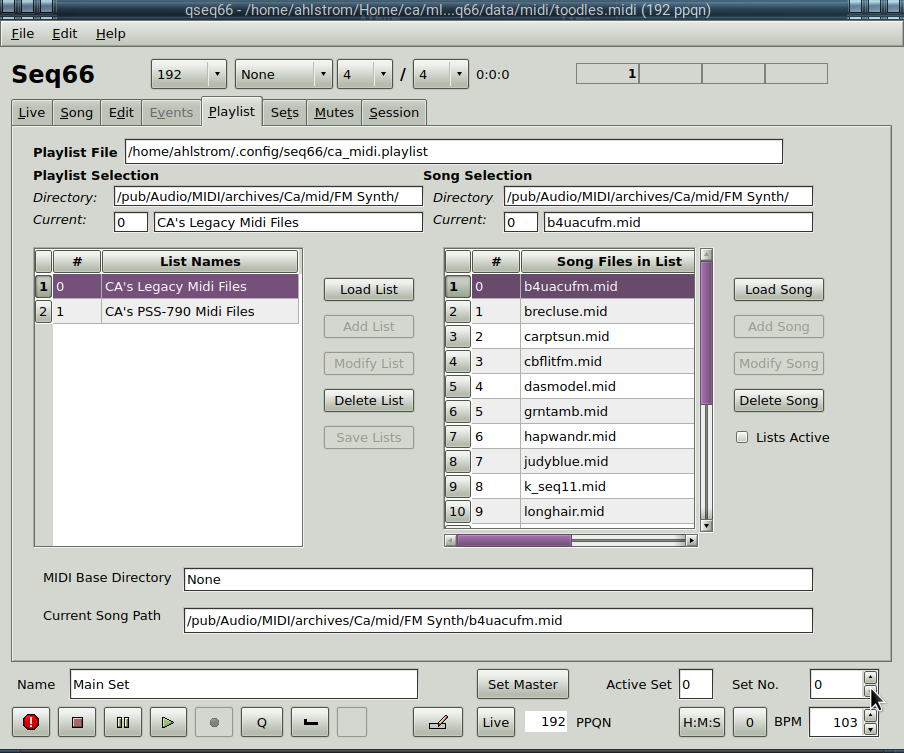
\includegraphics[scale=0.65]{playlist/personal-playlist-light.png}
   \caption*{Qt 5 Playlist Tab}
\end{figure}

   There is a lot to talk about in this tab.

   \begin{enumber}
      \item \textbf{Playlist File}.
         This field displays the path to the loaded
         play-list file.  It is not editable.  Remember that
         a play-list file can contain multiple play-lists.
      \item \textbf{Playlist Selection}.
         These fields display the main MIDI-file directory,
         the MIDI control number, and the name of the selected play-list.
         The \textbf{Directory} is where the MIDI files reside by default.
         A file-name can include a different path, however.
         These fields are editable, with the intent to use them to add a new
         play-list or modify the current one.
      \item \textbf{Song Selection}.
         These fields display the MIDI-file directory,
         the MIDI control number, and the file-name of the selected play-list.
         Note that the directory is normally the play-list directory, but a
         path present in the MIDI file-name overrides that directory.
         These fields are editable, with the intent to use them to add a new
         song or modify the "meta information" of the current one.
      \item \textbf{List Names}.
         This table shows the MIDI-control number and
         the name of each play-list.
      \item \textbf{List Buttons}.
         These buttons are described below.
         Please note that, in some cases, the exact functionality is still
         being worked out or perfected.
      \item \textbf{Song Files in List}.
         This table shows the MIDI-control number and
         the name of each song.
      \item \textbf{Song Files in List Buttons}.
         These buttons are described below.
         Please note that, in some cases, the exact functionality is still
         being worked out or perfected.
   \end{enumber}

\paragraph{Seq66 Play-Lists / User Interfaces / Playlist Buttons}
\label{paragraph:playlist_ui_qt_playlist_buttons}

   This section briefly describes the "List" buttons to the right of the
   play-list table.

   \begin{enumber}
      \item \textbf{Load List}.
   \end{enumber}

%-------------------------------------------------------------------------------
% vim: ts=3 sw=3 et ft=tex
%-------------------------------------------------------------------------------


% Set Master

%-------------------------------------------------------------------------------
% seq66 setmaster
%-------------------------------------------------------------------------------
%
% \file        seq66 setmaster.tex
% \library     Documents
% \author      Chris Ahlstrom
% \date        2020-01-13
% \update      2023-11-11
% \version     $Revision$
% \license     $XPC_GPL_LICENSE$
%
%     Provides a discussion of the MIDI GUI setmaster that Seq66
%     supports.
%
%-------------------------------------------------------------------------------

\section{Seq66 Set Master}
\label{sec:setmaster}

   The \textbf{Set Master} is a way to get a global view of all the screensets
   in a \textsl{Seq66} MIDI file, and to be able to do some simple operations
   (movement, naming, etc.) with the sets.
   In the latest version of \textsl{Seq66}, there are always 32 sets.
   This simplifies the handling of sets.
   Some sets may be empty.

\begin{figure}[H]
   \centering 
   \includegraphics[scale=0.75]{tabs/sets/setmaster-tab.png}
   \caption{Sets Tab}
   \label{fig:setmaster_tab}
\end{figure}

   The operations that can be done consist of viewing the sets, making a
   screenset active, rearranging the sets, clearing sets, and getting a survey
   of the contents of the sets.

   \setcounter{ItemCounter}{0}      % Reset the ItemCounter for this list.

   \itempar{Sets Grid}{set master!grid}
   The set grid is always 4 x 8.  Like the mute-groups, there's not
   a lot of benefit supporting more sets.  The reader may wish to email us
   arguing for a different point of view.
   \index{play screen}
   This grid shows the non-empty sets that are present in the MIDI file,
   represented by enabled buttons.
   With \textbf{Triggers} mode set, this  allows one to choose which set
   is currently
   active (i.e. which is the "play screen").
   Click on it and it is active.
   Also remember that keystrokes (\texttt{[} and \texttt{]} by default)
   in the main window can move the playscreen to the previous or next set.
 
   \itempar{Set List}{set master!list}
   The table at the right shows the set numbers, how many patterns/sequences
   are in each set, and the set name.  The set name is editable once it is
   double-clicked.

   \itempar{Set Number/Name Fields}{set master!number/name}
   Currently just shows the number and name of the selected set.
   Eventually, these fields will be editable.

   \itempar{Up/Down Buttons}{set master!up/down buttons}
   These buttons allow the user to move the selected set up and down
   in the list.

   \itempar{Show Set Info}{set master!show set info}
   Clicking this button lists all the sets and their tracks in the
   read-only edit box at the left.

   \itempar{Clear Set}{set master!clear set}
   Clicking this button deletes the patterns from the 
   set selected in the table.
   Note that the 0th set cannot be cleared.
   Would one ever want to do that?
   In \textsl{Seq66}, there must always be a set 0.

   \itempar{Triggers}{set master!set triggers}
   This checkable button toggles the action done by clicking a button
   in the set grid.
   If checked, then clicking an active set button will make that
   set active during playback.
   That effect depends on whether the sets are configured to auto-arm when
   selected, or not.
   If not checked, then clicking an active set button merely summarizes the
   patterns in the set, in the text field below the set grid.

   \itempar{Set 0}{set master!set 0}
   If trigger mode is in effect, clicking this button makes
   set 0 active.
   An alternative to clicking on grid button 0.

\subsection{Set Handling}
\label{subsec:setmaster_handling}

   This section talks about how sets work.  The topics are

   \begin{itemize}
      \item \textbf{Set Management}
      \item \textbf{Empty-Set Handling}
   \end{itemize}

\subsubsection{Set Management}
\label{subsubsec:setmaster_management}

   This section will discuss the work-flows of using sets to organize a song
   and to control playback.  MORE TO COME.

\subsubsection{Empty Set Handling}
\label{subsubsec:setmaster_empty_sets}

   When \textsl{Seq66} loads a song, it loads the existing sets in the song and
   sets their names as stored in the \texttt{c\_notes} \textsl{SeqSpec}
   (see \sectionref{subsec:midi_format_meta_format}).
   In addition, one dummy and invisible set is created for internal management
   purposes.

   When a new song is created, one usable set, Set \#0, is always created, as a
   starting point.  One generally starts with this set and adds patterns to it.

   When one selects the next set (e.g. using the \textbf{Live} frame's
   \textbf{Set} spin control), that set does not exist, but is immediately
   created.  So now the song has two sets, with the second one being empty.
   If the song is now saved, so is the empty set's file name.  However, empty
   sets are not saved; a set must be populated with at least one pattern to be
   saved.

   The following figure shows what happens when a song with 4 sets (0, 1, 2,
   and 7) is loaded, and then the user increments the spin-button all the way
   to set 8.

\begin{figure}[H]
   \centering 
   \includegraphics[scale=0.85]{tabs/sets/setmaster-with-additional-sets.png}
   \caption{New Sets Creation}
   \label{fig:setmaster_set_creation}
\end{figure}

   There are new sets 3, 4, 5, 6, and 8.  However, if one saves and then
   reloads this song, the empty sets are gone.  Just something to be aware of.

%-------------------------------------------------------------------------------
% vim: ts=3 sw=3 et ft=tex
%-------------------------------------------------------------------------------


% Mutes and mute-groups

%-------------------------------------------------------------------------------
% seq66 mutes
%-------------------------------------------------------------------------------
%
% \file        seq66 mutes.tex
% \library     Documents
% \author      Chris Ahlstrom
% \date        2020-01-13
% \update      2023-04-14
% \version     $Revision$
% \license     $XPC_GPL_LICENSE$
%
%     Provides a discussion of the MIDI GUI mutes that Seq66
%     supports.
%
%-------------------------------------------------------------------------------

\section{Seq66 Mutes Master}
\label{sec:mutes_master}

   The \textbf{Mutes} tab is a way to get a global view of all the mutegroups in
   a \textsl{Seq66} MIDI file or global configuration, and to be able to do
   some simple operations with the mute groups.
   A mute-group holds the statuses (armed/muted) of all of the patterns in
   a screenset (see \sectionref{subsubsec:concepts_terms_bank}).
   A mute-group can be associated with a hot-key (or MIDI control), so that,
   when the mute-group is selected, the patterns that are armed changes.
   This makes it easy to change what the tune is playing in a big way.
   Mute-groups are \textsl{learned} by

   \begin{enumerate}
      \item Arming all of the desired pattern in the set.
      \item Clicking the \textbf{Learn} ("L") button.
      \item Clicking the keystroke, which is almost always the shifted version
         of the hot-key to arm/mute the pattern.
         This is accomplished in the default keyboard configuration via the
         \index{auto-shift}
         auto-shift function, which shifts the keystroke automatically
         for group-learn.
   \end{enumerate}

   These steps can also be done via MIDI control.

   To learn more about mute-groups, see
   \sectionref{subsubsec:introduction_mute_group_learn_button}, and
   \sectionref{subsubsec:concepts_terms_group}.

% TODO: UPDATE THIS FIGURE WITH THE LATEST.

\begin{figure}[H]
   \centering 
   \includegraphics[scale=0.75]{tabs/mutes/mute-master-tab.png}
   \caption{Mutes Tab}
   \label{fig:mutes_master_tab}
\end{figure}

   This diagram show the \textbf{Mutes} tab after some mute-groups have been
   created.  Mute-groups can be created in the main window's patterns panel,
   but it is difficult to know what each group consists of.  This tab make it
   easy to see the layout of the mute-groups, and also allows for some editing
   of the mute-groups.

   \setcounter{ItemCounter}{0}      % Reset the ItemCounter for this list.

   \itempar{Group Table}{mutes!table}
   At the right is a table that holds all of the assigned mute-group key and
   some information about them:

      \begin{itemize}
         \item \textbf{Group}.
            This column holds the group numbers for each group, ranging from 0
            to 31.  Each row corresponds to a buton in the \textbf{Mute-Groups}
            grid.
         \item \textbf{Active}.
            This column shows the number of activated patterns in the
            mute-group.  A zero means the mute-group is inactive.
         \item \textbf{Key}.
            Indicates the keystroke that can be used to put that mute-group in
            place on the patterns in the current screenset.
            By default, these are shifted version of the corresponding
            mute/unmute pattern-slot hotkey.
         \item \textbf{Group Name}.
            Provides a mnemonic name for the mute group.  A feature for the
            future.
      \end{itemize}

   Currently, only the \textbf{Group Name} field is editable directly.
   The user generally should modify (tweak)
   \texttt{qseq66.mutes} with a text editor.
   This table is the only way to select a mute-group for editing.
   Click on the desired group, and then click on the group button, perhaps
   twice, to be able to add pattern mute states via the pattern buttons.

   \itempar{Mute-Groups}{mutes!groups}
   This grid is always of size \textbf{4 x 8}.  It represents the maximum of 32
   mute-groups that can be supported by \textsl{Seq66}.
   To start, all group buttons are \textsl{disabled} and
   \textsl{unchecked} (inactive).
   Where a mute-group exists, the button is made \textsl{checked} (active),
   but still disabled.

   Here, the user clicked on mute-group 7, which now becomes active in the
   user-interface.  (But it is not made active in the patterns panel).
   The \textbf{7} button is also enabled, and can be clicked.

   Clicking once deactivates the button, which potentially flags that mute-group
   for removal.  Clicking it again reactivates it, which also enables all of the
   buttons in the \textbf{Group Patterns} grid.

   \itempar{Group Patterns}{mutes!patterns}
   Once this grid is enabled, each button can be click to add a pattern to the
   mute-group, or remove a pattern from the mute-group.

   \itempar{Update Group}{mutes!update group}
%
%  Was "Set Mutes"
%
   When a change in the mute-group status or the status of one of its patterns
   is made, this button becomes enabled.  Once clicked, the current mute-group
   is modified internally, where it will later be saved when \textsl{Seq66}
   exits, or when the \textbf{Save All} button is clicked.

   \itempar{Mutes File}{mutes!mutes file}
   The mutes-file shows the base-name of a file into which one can write the
   current-mute group setup, as a way to back up the setup.
   TO DO:  We need to disable auto-save of the mutes file at exit in this case,
   unless the name provided is identical.

   \itempar{Save All}{mutes!save all}
%
%  Was "Save File"
%
   This button saves all of the mute-groups.
   It is enabled when a change has been made to a mute-group and
   has been registered by pressing the \textbf{Update Group} button.
   If the user has provided a path in the \textbf{Mutes File} field, the path
   is stripped.  We do not want to write configuration information outside of
   the session configuration directory.
   The file is saved, but is not made official in the
   'rc' file; one must edit the 'rc' file to use the new 'mutes' file.
   We might provide a button for that function at some point.

   \itempar{Write Format}{mutes!write format}
   This section provides the following features, which still need some work:

      \begin{itemize}
         \item \textbf{Binary}.
            This flag indicates to save the mute-group information in
            binary format, which is the normal format.
            Each mute-group pattern's setting is indicated by a 0 or a 1.
            This is the default format for writing the mute-groups.
         \item \textbf{Hex}.
            In this format, each set of mute-group is written in 8-bit hexadecimal
            format (e.g. "0xff").  This format is useful if the user has opted to
            have large set sizes such as 64 and 96 patterns.  Not well-supported
            yet.
         \item \textbf{To MIDI}.
            When a tune is closed, as when \textsl{Seq66} exits, this option
            indicates to write the mute-group information to the
            \textsl{Seq66}-style MIDI file.
         \item \textbf{To Mutes}.
            When a tune is closed, as when \textsl{Seq66} exits, this option
            indicates to write the mute-group information to the normal
            \textsl{Seq66} configuration file (e.g. \texttt{qseq66.mutes}).
      \end{itemize}

   \itempar{Trigger Mode}{mutes!trigger mode}
      When activated, this option will enable the \textbf{Mute-Groups} buttons,
      deactive them all, and turn them into standard push-buttons.  When clicked
      the mute-group will be actived during playback.

   \itempar{Clear}{mutes!clear all mutes}
      This button will clear every mute group. Use it carefully!

   \itempar{Fill}{mutes!fill mutes}
      This button will create a set of empty mute-groups.
      Currently, this alters the current MIDI tune, forcing a prompt to save.
      This action creates 32 empty mute-groups.
      If a single mute-group is created in the patterns panel,
      then only that mute-groups is saved.

% INVESTIGATE!!!

   \itempar{Pattern Offset}{mutes!pattern offset}
      If the user has selected a larger set size that is a multiple of 32, this
      item is enabled.  It then allows the user to modify patterns with a
      sequence number greater than 31.  A future feature.

   \itempar{Up/Down Buttons}{mutes!up/down buttons}
      A future feature to move mute-group around without
      changing the keystroke for that mute group.

%-------------------------------------------------------------------------------
% vim: ts=3 sw=3 et ft=tex
%-------------------------------------------------------------------------------


% Palettes

%-------------------------------------------------------------------------------
% palettes
%-------------------------------------------------------------------------------
%
% \file        palettes.tex
% \library     Documents
% \author      Chris Ahlstrom
% \date        2020-12-29
% \update      2023-03-23
% \version     $Revision$
% \license     $XPC_GPL_LICENSE$
%
%     Provides a discussion of the MIDI GUI palettes that Seq66
%     supports.
%
%-------------------------------------------------------------------------------

\section{Palettes for Coloring}
\label{sec:palettes}

   Many user-interface elements in \textsl{Seq66} are drawn independently of
   the Qt theme in force, and they have their own coloring.  Also, patterns can
   be colored, and the color is stored (as a color number) in the pattern when
   the tune is saved.
   There are four palettes:

   \begin{itemize}
      \item \textbf{Pattern}.  This palette contains 32 color entries, and each
         can be used to add color to a pattern in the \textsl{Live} grid or in
         the \textsl{Song} editor.  The color of a pattern, if used, is saved
         with the pattern in the MIDI file.
      \item \textbf{Ui}.  This palette contains 16 color entries.  These
         color entries are used in drawing text, backgrounds, grid lines,
         background patterns, drum notes, and more.  These colors each have a
         counterpart that is used with the \texttt{-{}-inverse} option is applied
         to a run of \textsl{Seq66}.
      \item \textbf{Inverse Ui}.  This palette contains 16 color entries.
         These colors are used when the \texttt{-{}-inverse} option is applied
         to a run of \textsl{Seq66}.
      \item \textbf{Brushes}.  This "palette" provides a way to specify the
         fill type for the drawing of notes, the scale (if shown) in the
         pattern editor, and the background sequence (if shown).  It allows the
         user to select solid file, hatching, and some other fill patterns.
   \end{itemize}

   All palettes have default values built into the application.  However, the
   user can also include 'palette' files to change the colors used.  For
   example, the normal colored palette can be changed to a gray-scale palette.
   The name of the palette file is specified in the 'rc' file by lines like the
   following:

   \begin{verbatim}
      [palette-file]
      1     # palette_active
      qseq66-alt-gray.palette
   \end{verbatim}

   If this palette file is active, it is loaded, changing all of the palettes,
   and thus the coloring of \textsl{Seq66}.
   In \sectionref{subsec:palettes_theming}, some weird behavior with
   the \texttt{qt5ct} configuration application and non-Qt-based window managers
   is discussed.

\subsection{Palettes Setup}
\label{subsec:palettes_setup}

   The palette file is a standard \textsl{Seq66} configuration file with a name
   something like \texttt{qseq66.palette}, plus two sections:

   \begin{verbatim}
      [palette]
      [ui-palette]
   \end{verbatim}

   The first section is the "Pattern" palette, and the second section is the
   "Ui" palette, which includes the inverse palette as well.

\subsubsection{Palettes Setup / Pattern}
\label{subsubsec:palettes_setup_pattern}

   The following shows the pattern palette, with some entries elided for
   brevity:

   \begin{verbatim}
      [palette]
       0            "Black" [ 0xFF000000 ]      "White" [ 0xFFFFFFFF ]
       1              "Red" [ 0xFFFF0000 ]      "White" [ 0xFFFFFFFF ]
       2            "Green" [ 0xFF008000 ]      "White" [ 0xFFFFFFFF ]
       3           "Yellow" [ 0xFFFFFF00 ]      "Black" [ 0xFF000000 ]
       4             "Blue" [ 0xFF0000FF ]      "White" [ 0xFFFFFFFF ]
       ...            ...       ...             ...       ...
      29      "Dark Violet" [ 0xFF9400D3 ]      "Black" [ 0xFF000000 ]
      30       "Light Grey" [ 0xFF778899 ]      "Black" [ 0xFF000000 ]
      31        "Dark Grey" [ 0xFF2F4F4F ]      "Black" [ 0xFF000000 ]
project.
   \end{verbatim}

   The names are color names, and these names are what show up in the popup
   color menus for the pattern buttons in the \textsl{Live} grid.
   The colors on the left are the background colors, and the colors on the
   right are the foreground colors, which are chosen for contrast with the
   background.  The colors are in \texttt{\#AARRGGB} format, with the "\#"
   replaced by "0x" because "\#" starts a comment in \textsl{Seq66}
   configuration files.  Note that all the alpha values are "FF" (opqque); we
   have not yet experimented with changing them.
   Lastly, only 32 entries are accepted.

\subsubsection{Palettes Setup / Ui and Inverse Ui}
\label{subsubsec:palettes_setup_ui}

   The following shows the pattern palette, with some entries elided for
   brevity:

   \begin{verbatim}
      [ui-palette]
       0       "Foreground" [ 0xFF000000 ] "Foreground" [ 0xFFFFFFFF ]
       1       "Background" [ 0xFFFFFFFF ] "Background" [ 0xFF000000 ]
       2            "Label" [ 0xFF000000 ]      "Label" [ 0xFFFFFFFF ]
       3        "Selection" [ 0xFFFFA500 ]  "Selection" [ 0xFFFF00FF ]
       4             "Drum" [ 0xFFFF0000 ]       "Drum" [ 0xFF000080 ]
             ...            ...       ...       ...       ...
      13        "Beat Line" [ 0xFF2F4F4F ]  "Beat Line" [ 0xFF2F4F4F ]
      14        "Step Line" [ 0xFF778899 ]  "Step Line" [ 0xFF808080 ]
      15            "Extra" [ 0xFF778899 ]      "Extra" [ 0xFFBD6BB7 ]
   \end{verbatim}

   Here, the names are feature names, not color names.  The first color is the
   normal color, and the second color is the inverse color.  Only 16 entries
   are accepted.

\subsubsection{Palettes Setup / Brushes}
\label{subsubsec:palettes_setup_brushes}

   The last palette is small, allowing the fill-pattern of a few pattern-editor
   items to be changed.

   \begin{verbatim}
      [brushes]
      empty = solid              # preferred
      note = lineargradient      # default
      scale = dense3
      backseq = dense2
   \end{verbatim}

   On the left of the equals sign is the item than can be filled, and on the
   right side is the \textsl{Qt} brush to be used.  The defaults for most are
   solid fill.

   The entry \texttt{empty} isn't too useful; best to leave it set to 'solid'.
   The entry \texttt{note} affects the fill of normal/selected notes.
   The best values are either 'lineargradient' (the default) or 'solid'.
   The entry \texttt{scale} affects the fill for the piano roll scale.  The
   hatching used here makes it easier to recognize that the scale is just there
   for orientation.
   The entry \texttt{backseq} affects the fill of the background sequence.  The
   hatching used here helps further distinguish the real notes from the
   background notes.

\subsection{Palettes Summary}
\label{subsec:palettes_summary}

   There are some obvious enhancements to this scheme, including increasing the
   number of palette items, synchronizing the palette with the current desktop
   them semi-automatically, and providing a user interface to drag-and-drop
   colors.

\subsection{Theming}
\label{subsec:palettes_theming}

   When using a non-Qt-based window manager or desktop manager, such as our
   favorite, \textsl{Fluxbox}, in conjunction with \textsl{GTK+} themes,
   there can be issues on some \textsl{Linux} distros.

   First, if using a Gtk theme setter (e.g. \textsl{gtk-chtheme}), one wants to
   use \textsl{qt5ct} to set Qt to work with Gtk themes.
   For this to work well, use this setting in the \texttt{.bashrc} or
   \texttt{.profile} file:

   \begin{verbatim}
      export QT_QPA_PLATFORMTHEME=gtk2
   \end{verbatim}

   If not, use the following setting:

   \begin{verbatim}
      export QT_QPA_PLATFORMTHEME=qt5ct
   \end{verbatim}

   Another option is to provide an executable script like the following,
   giving it a name such as \texttt{dseq66}
   (for a dark themed \textsl{Seq66}) to
   distinguish it from the normal-themed \texttt{qseq66}.

   \begin{verbatim}
      #!/bin/sh
      # Use dark coloring on qseq66, as we have configured in qt5ct.
      QT_QPA_PLATFORMTHEME=qt5ct qseq66
   \end{verbatim}

   One might still encounter the issue that, with a Gtk theme, applications
   take about 20 to 30 seconds to start up!
   More information to come.
   Also see the style-sheet discussion in
   \sectionref{sec:configuration}.

%-------------------------------------------------------------------------------
% vim: ts=3 sw=3 et ft=tex
%-------------------------------------------------------------------------------


% Tables of keyboard and mouse actions

%-------------------------------------------------------------------------------
% kbd_mouse
%-------------------------------------------------------------------------------
%
% \file        kbd_mouse.tex
% \library     Documents
% \author      Chris Ahlstrom
% \date        2016-04-07
% \update      2021-01-13
% \version     $Revision$
% \license     $XPC_GPL_LICENSE$
%
%     Provides tables for keyboard and mouse support in Seq66.
%
%-------------------------------------------------------------------------------

\section{Seq66 Keyboard and Mouse Actions}
\label{sec:kbd_mouse_actions}

   This section presents some tables summarizing keyboard and mouse actions
   available in \textsl{Seq66}.
   It does not cover mute keys and group keys, which are well
   described in the keyboard options for the main window.
   It does not cover the "fruity" mouse actions, as this mode of mouse-handling
   is not supported in \textsl{Seq66}.

%  Any volunteers to fill in the table?

   This section describes the keystrokes that are currently hardwired
   in \textsl{Seq66}.
   This description only includes items not defined in the 'ctrl' file.
   That is, hardwired values.
   "KP" stands for "keypad".
   \index{keys!focus}
   The effect that keystrokes have depends upon
   which window has the keyboard/mouse focus.
   \index{keys!qt}
%  It must be noted that the Qt 5 user-interface still has a few missing pieces
%  in keystroke support.

\subsection{Keyboard Control}
\label{subsec:kbd_mouse_keyboard_control}

   \textsl{Seq66} provides a plethora of keyboard controls for user-interface
   actions, note-modification, zooming, and pattern control.
   Most of these controls (not all)
   are easy to change by editing the appropriate 'ctrl'
   configuration file, stored in one of the following directories, depending on
   the operating system:
   
   \begin{verbatim}
      /home/username/.config/seq66/qseq66.ctrl
      C:/Users/username/AppData/Local/seq66/qpseq66.ctrl
   \end{verbatim}

   There are also some extended examples present in the \textsl{Seq66}
   \texttt{data/linux} and
   \texttt{data/samples} directory.
   Note that keyboard and MIDI control settings have been consolidated
   into a single table in the 'ctrl' file.
   The \texttt{[mute-group]} control
   section has been moved to it's own 'mutes' file.

   \index{keys!gotchas}
   There are a number of "gotchas" to be aware of when assigning keys to the
   fields in the \textbf{Keyboard} tab:

   \begin{itemize}
      \item Some of the keystrokes are hard-wired, such as 
         "arrow" keys (for controlling play-lists), "page up/down" keys, or
         the "zoom" keys.
      \item \textsl{Seq66} has appropriated the
         \index{keys!shift} Shift key so that a a Shift-left-click on a pattern
         slot opens up the corresponding set (based on pattern number)
         in an external live grid.
         \index{auto-shift}
         For the group-learn feature, the \texttt{Shift} key is 
         automatically enabled, using an "auto-shift" feature.
         Thus, using characters that require the Shift
         key while clicking, such as \texttt{\{} and \texttt{\}},
         becomes surprising.
         Instead, look to the remaining keys: \texttt{F11}, \texttt{F12},
         and the "keypad" keys if more keystrokes are wanted.
   \end{itemize}

   \texttt{[keyboard-control]}.
   We won't attempt to cover every key-control item,
   just the categories.  Some items might be discussed in other parts
   of this manual. Remember that key and MIDI control have been consolidated.
   Also remember that the 'ctrl' file contains comments and an orderly layout
   to make it easier to understand and to edit.

   \index{pause}
   An additional key definition is shown for the pause key.
   By default, the pause key is the period
   ("\texttt{.}."), but that can be changed.

   \index{pattern edit}
   A goal of \textsl{Seq66} is being able to edit a pattern using mainly the
   computer keyboard.
   \textsl{Seq66} supports two modifier keys.
   The first modifier key causes the usual pattern-toggle key (hot-key) for a
   given slot to instead bring up the pattern editor.  By default, this key is
   the equals ("\texttt{=}") key.
   \index{event edit}
   The second modifier key causes the usual
   pattern-toggle key (hot-key) for a given slot to instead bring up the event
   editor.  By default, this key is the minus ("\texttt{-}") key.
   Both of these keys are configurable.

   Some of the keys have positional mnemonic value.  For example,
   for BPM control, the semicolon is at the left (down), and the apostrophe
   is at the right (up).

   \index{slot-shift}
   \index{keys!slot-shift}
   The \textbf{slot shift} key is useful when using pattern grids larger
   than 8 x 4 patterns.  Pressing the slot-shift key basically adds 32 to the
   pattern number of the slot-key that is pressed.
   The default key is the forward slash ("\texttt{/}") key.

   \index{snapshot}
   \index{keys!snapshot}
   A \textbf{snapshot} is a briefly-preserved state of the patterns.
   One can press a snapshot key, change the state of the patterns for live
   playback, and then release the snapshot key to revert to the state when
   the snapshot key was first pressed.
   The default key is the \texttt{Ins} key.

%   Holding 'Alt' will save the state of playing sequences
%   and restore them when 'Alt' is lifted.
%
%   Holding 'Left Ctrl' and 'Alt' at the same time will enable
%   you to flip over to new sequences briefly and then
%   flip right back upon lifting 'Alt'.
%
%	Is this Snapshot 1 versus Snapshot 2?  In Seq24's code, either key
%  does exactly the same thing!

   \index{queue}
   \index{keys!queue}
   To \textbf{queue}
   a pattern means to ready it for playback upon the next repeat
   of a pattern.  A pattern can be armed immediately with a hot-key,
   or it can be queued to play back the next time the pattern repeats.
   A pattern can be queued by holding the queue key (defined in
   \textbf{File / Options / Keyboard / queue}) and pressing a pattern-slot
   hot-key.  Instead of the pattern turning on
   immediately, it turns on at the next repeat of the pattern.
   The default key is the "\texttt{o}" key.

   \index{keep queue}
   \index{keys!keep queue}
   \index{queue!keep}
   \textbf{Keep queue}
   allows the queue to be held without holding
   down the queue button the whole time.  First, press the keep-queue key.
   Next, hitting
   any of the slot hot-keys, no matter how many, sets up the corresponding
   pattern slot to be queued.  Also, in keep-queue mode, clicking on the
   pattern slot will queue the pattern.  The keep-queue mode is disabled by
   hitting the "queue" key again (any currently active queues remain active
   until finished).
   The default key is the backslash key, "\texttt{\textbackslash}" key.
   There is also a "Q" button to toggle the keep-queue
   status.

   \index{one-shot}
   \index{keys!one-shot}
   \textbf{One-Shot}
   causes a slot to be queued for only a single playback.
   The default key is the pipe, "\texttt{|}" key.
   Currently buggy.

   \itempar{Sequence toggle keys}{keyboard!sequence toggle keys}
   Each of these keys toggles the playing/muting of one of the 32
   loop/pattern boxes.
   These keys are layed out logically on the keyboard by default,
   and can also be shown in each loop/pattern box.
   Please note that we often call them "shortcut keys" or "hot-keys"
   where the context
   makes it clear that they apply to the armed/unarmed state of a pattern.

   \itempar{Mute-group slots}{keyboard!mute-group slots}
   There can be up to 32 mute-groups.
   \index{playing set}
   When activated, a mute-group
   sets the muted/unmuted status of the current "playing set"
   to the pattern-muting statuses of the selected mute-group.
   Each of these keys operates on the mute-grouping of one of the 32
   stored mute groups.
   These keys are layed out logically on the keyboard by default, and consist
   of \texttt{Shift} versions of the sequence-toggle (hot) keys.
   Note that a mute-group key will be memorized only when
   \textsl{Seq66} is in
   \index{group-learn}
   \textsl{group-learn} mode.

%  \index{mute-group}
%  One thing to explain is just what mute-grouping means.
%  \textsl{Mute groups} are shortcuts to play a defined group of patterns
%  on the current set, while stopping other patterns from the current set, and
%  all patterns from other sets.

   \itempar{Learn}{keyboard!learn}
   \index{group!learn}

   To define the group of patterns for one mute group, press and hold the
   configured Learn key (the "el", "\texttt{l}" key by default,
   the hard-wired \texttt{Ctrl-L} key, or the "\textbf{L}"
   button in the user-interface.
   Then pressing one of the mute group keys
   will save the currently-playing pattern slots into the corresponding mute
   group.
   \index{auto-shift}
   The default mute group keys must be the shifted version of the key,
   but one should not press the \texttt{Shift} key for this key.
   \textsl{Seq66} will automatically assign the corresponding key with
   \texttt{Shift} activated.

   Note that, once in learn-mode, there is no way to cancel learn-mode
   except by selecting an illegal mute-group keystroke.
   Also see \sectionref{sec:mutes_master}.

%  TO BE FIXED
%  Group-mute can be globally enabled or disabled (with default keys apostrophe
%  \texttt{'} \index{grave} \index{igrave} and igrave or grave \texttt{`}).
%  So make sure it is enabled before trying to use it.

   \itempar{Disable}{keyboard!disable}
   \index{keys!apostrophe}
   It is the inverse \textbf{apostrophe} key by default.
   \index{group!off}
   \index{keyboard!group off}
   This key is the \textsl{group off} key.

   \itempar{Enable}{keyboard!enable}
   \index{keyboard!igrave}
   It is the \textbf{igrave} (back-tick) key by default.
   \index{group!on}
   \index{keyboard!group on}
   This key is the \textsl{group on} key.

   A number of additional functions have been added to \textsl{Seq66},
   and keystrokes have been provided for those new functions.

   \setcounter{ItemCounter}{0}      % Reset the ItemCounter for this list.

   \index{song mode}
   Note the \textbf{Song/Live toggle} key.
   The \textsl{song mode} normally is in effect only when playback is started
   from the \textbf{Song Editor}.  Now this mode can be used from any
   window, if enabled by pressing this key.  There is also
   a button in the main window for this function, which shows the current state
   of this flag.  Note that this flag is also stored in the 'rc' configuration
   file, as well as this hot-key value, which defaults to \texttt{F10}.

   \index{toggle JACK}
   \index{JACK toggle}
   The \textsl{JACK mode} is set via the
   \textbf{File / Options / JACK / JACK Connect} or 
   \textbf{JACK Disconnect} buttons.
   This keystroke will toggle between JACK connect and JACK disconnect.
   The \textbf{Song Editor} will also have a \textbf{JACK} button.
   The hot-key for this function defaults to \texttt{F2}.

   \index{menu mode}
   The \textsl{menu mode} indicates if the main menu of the
   main window is accessible or not.  It is disabled during playback
   so that more hot-keys can be used without triggering menu functions.
   It can also be disabled by the user; the default hot-key is \texttt{F3}.
   This feature is needed because the original \textsl{Seq24} had numerous
   conflicts between the menu key bindings and the default key bindings for the
   main window.

%  Here is Stazed's explanation of the feature, mildly edited:
%
%  \begin{quotation}
%     \textsl{"why disabling is needed when playing"}
%     The original seq24 had numerous conflicts between the menu key binding
%     and the default seq24 key binding for the mainwind sequence triggers.
%     For example: Ctrl-q (quits the program without prompt). If you place a
%     sequence in the default 'q' slot, you cannot use it with Ctrl-l or Ctrl-r
%     (default replace or queue) because the menu grabs the keys. Same goes for
%     the Alt-l or Alt-r (default snapshot 1 or 2). Try same as above with
%     Alt-f, Alt-v, Alt-h, Ctrl-n, Ctrl-o...  etc. So I just shut off all the
%     menus by default when playing because it seems that they should not be
%     needed then... especially in a live performance.
%
%     \textsl{"why a button?"}
%     On occasion I wanted to use the mainwnd key binding when stopped to set
%     the sequences to be ready before starting. It's also a sort of safety
%     feature as well, just toggle the menus off before going live so that you
%     don't hit Ctrl-q, Ctrl-n etc. forgetting things are not playing....
%  \end{quotation}

   \index{follow jack}
   \textsl{Follow JACK} is a feature ported from \textsl{Seq32}.
   The default key is \texttt{F4}.
   It determines if \textsl{Seq66} follows JACK transport.

   \index{fast forward}
   \textsl{Fast forward} is a feature ported from \textsl{Seq32}.
   The default key is \texttt{F6}.
   While this key is held, the song pointer will fast-forward
   through the song.
   This feature does not have a corresponding button.

   \index{rewind}
   \textsl{Rewind} is a feature ported from \textsl{Seq32}.
   The default key is \texttt{F5}.
   While this key is held, the song pointer will rewind.
   This feature does not have a corresponding button.

   \index{pointer position}
   \textsl{Pointer position} is a feature ported from \textsl{Seq32}.
   The default key is \texttt{F7}.
   When this key is pressed, the song pointer will move to the
   current position of the mouse, snapped.
   This feature does not have a corresponding button.

   \index{toggle mutes}
   \textsl{Toggle mutes} toggles the mute status of every
   pattern on every screen-set.  It corresponds to the
   \textbf{Edit / Toggle mute all tracks} or the 
   \textbf{Song / Toggle All Tracks}
   menu entries.  There is also a button in the main window for this function,
   which shows the current state of this flag.  Note that this
   hot-key value is stored in the 'rc' configuration file, and
   defaults to \texttt{F8}.

   \index{tap bpm}
   \textsl{Tap BPM} allows the user to "tap" in time with some
   other music, and see the tap sequence translated into beats/minute (BPM).
   There is also a "0" button for this function.
   After 5 seconds, this feature resets automatically, so the user can try
   again if not satisfied.  At least two taps are needed for the
   BPM to be registered.

% VERIFY and the UNCOMMENT
%
%  Tap BPM causes events to be logged to the tempo track which is the first
%  track (track 0) by default.

\subsection{Main Window}
\label{subsec:kbd_mouse_main_window}

   The main window keystrokes are all defined via the options dialog
   and "rc" configuration file, or are stock window-management keystrokes.
   The main window has a very complete setup for live control of the MIDI tune
   via keystrokes.  These actions are not included in
   \tableref{table:main_window_support}.
%  There may be some other keystrokes to be documented at some point.

   \begin{table}[H]
      \centering
      \caption{Main Window Support}
      \label{table:main_window_support}
      \begin{tabular}{l l l l l l}
         \textbf{Action} & \textbf{Normal} & \textbf{Double} & \textbf{Shift} & \textbf{Ctrl} \\
         \textbf{e} & --- & --- & --- & Open song editor \\
         \textbf{l} (el) & --- & --- & --- & Enter Learn mode \\
         Left-click slot & Mute/Unmute & New/Edit & Toggle other slots & --- \\
         Right-click slot & Edit menu & --- & Edit menu & Edit Menu \\
      \end{tabular}
   \end{table}

   The new mouse features of this window for \textsl{Seq66},
   as noted in \sectionref{sec:patterns_panel}, are:

   \begin{itemize}
      \item \textsl{Shift-left-click}:
         Over one pattern slot, this action toggles the mute/unmute
         (armed/unarmed) status of all other patterns
         (even the patterns in other, unseen sets).
      \item \textsl{Left-double-click}:
         Over a pattern slot, this action quickly toggles the mute/unmute status,
         which is confusing.  But it ultimately brings up the pattern editor
         (sequence editor) for that pattern.
%        It acts like Ctrl-left-click.
   \end{itemize}

\subsection{Performance Editor Window}
\label{subsec:kbd_mouse_performance_editor_window}

   The "performance editor" window is also known as the "song editor" window.
   It's main sections are the "piano roll" (perfroll) and the "performance
   time" (perftime) sections, discussed in the following sections.
   Also, some keystrokes are handled by the frame of the window.

   \begin{itemize}
      \item \texttt{Ctrl-z}. Undo.
      \item \texttt{Ctrl-r}. Redo.
   \end{itemize}

\subsubsection{Performance Editor Piano Roll}
\label{subsubsec:kbd_mouse_performance_editor_piano_roll}

%  \begin{itemize}
%     \item \texttt{Ctrl-x}. Cut.
%     \item \texttt{Ctrl-c}. Copy.
%     \item \texttt{Ctrl-v}. Paste.
%     \item \texttt{Ctrl-z}. Undo.
%     \item \texttt{Ctrl-r}. Redo.
%     \item \texttt{Shift-Up}.   Move backward one small unit (which is...?)
%     \item \texttt{Shift-Down}.   Move forward one small unit (which is...?)
%     \item \texttt{Shift-Page Up}.   Move backward one frame.
%     \item \texttt{Shift-Page Down}.   Move forward one frame.
%     \item \texttt{Shift-Home, Shift-KP Home}.  Move to beginning of piano roll.
%     \item \texttt{Shift-End, Shift-KP End}.  Move to end of piano roll.
%     \item \texttt{Shift-z (Z)}.  Zoom in.
%     \item \texttt{0}.  Set default zoom.
%     \item \texttt{z}.  Zoom out.
%     \item \texttt{Left}.  Move item left one snap unit.
%     \item \texttt{Right}.  Move item right one snap unit.
%     \item \texttt{Up}.  Move frame up one small scroll unit.
%     \item \texttt{Down}.  Move frame down one small scroll unit.
%     \item \texttt{Home}.  Move to top of piano roll.
%     \item \texttt{End}.  Move to bottom of piano roll.
%     \item \texttt{Page Up}.  Move up one frame (page-increment).
%     \item \texttt{Page Down}.  Move down one frame (page-increment).
%  \end{itemize}

   Note that the keystrokes in this table
   (see \tableref{table:perf_window_piano_roll})
   require that the focus first be
   assigned to the piano roll by left-clicking in an empty area within it.
   Otherwise, another section of the performance editor might receive the
   keystroke.

   \begin{table}[H]
      \centering
      \caption{Performance Window Piano Roll}
      \label{table:perf_window_piano_roll}
      \begin{tabular}{l l l l l l}
         \textbf{Action}   & \textbf{Normal} & \textbf{Double}    & \textbf{Shift}     & \textbf{Ctrl}  \\
         Space             & Start playback  & ---                & ---                & ---            \\
         Esc               & Stop playback   & ---                & ---                & ---            \\
         Period (.)        & Pause playback  & ---                & ---                & ---            \\
         Del               & Cut section     & ---                & ---                & ---            \\
         c key             & ---             & ---                & ---                & Copy           \\
         p key             & Paint mode      & ---                & ---                & ---            \\
         v key             & ---             & ---                & ---                & Paste          \\
         x key             & Escape paint    & ---                & ---                & Cut            \\
         z key             & Zoom out        & ---                & ---                & Undo           \\
         0 key             & Reset zoom      & ---                & ---                & ---            \\
         Z key             & Zoom in         & ---                & ---                & Undo           \\
         Left-arrow        & Move earlier    & ---                & ---                & ---            \\
         Right-arrow       & Move later      & ---                & ---                & ---            \\
         Left-click        & Select section  & ---                & ---                & ---            \\
         Right-click       & Paint mode      & ---                & Paint mode         & Paint mode     \\
         Scroll-up         & Scroll up       & ---                & Scroll Left        & Scroll Up      \\
         Scroll-down       & Scroll down     & ---                & Scroll Right       & Scroll Down    \\
      \end{tabular}
   \end{table}

   This section of the performance editor also handles the start, stop, and
   pause keys.  These can be modified in the \textbf{Options / Keyboard} page.
   A "section" in the performance editor is actually a box that
   specifies a trigger for the pattern in that sequence/pattern slot.
   Note that the "toggle other slots" action occurs only if shift-left-clicked
   in the "names" area of the performance editor.
   Left-click is used to select performance blocks if clicked within
   a block, or to deselect them if clicked in an empty area of the piano roll.
   Also note that all scrolling is done by the internal horizontal and vertical
   step increments.
   Some features of this window for \textsl{Seq66},
   as noted in \sectionref{sec:song_editor}, are explained here:

   \begin{itemize}
      \item \textsl{p}:  Enters the paint mode, until right-click is pressed or
         until the "x" key is pressed.
      \item \textsl{x}:  Exits the paint mode.  Think of the made-up term
         "x-scape".
      \item \textsl{z}:  Zooms out the performance view.  It makes the view
         look smaller, so that more of the performance can be seen.
         Opening a second performance view is another way to see more
         of the performance.
      \item \textsl{0}:  Resets the zoom to its normal value.
      \item \textsl{Z}:  Zooms in the performance view, making the view
         larger, so that more details of the performance can be seen.
%     \item \textsl{.}:  The period (configurable) is a new key devoted to the
%        new pause functionality.
      \item \textsl{Left Arrow}:  Moves the selected item to the left (earlier
         in time) in the performance layout.
      \item \textsl{Right Arrow}:  Moves the selected item to the right (later
         in time) in the performance layout.
      \item Once selected (rendered in grey), a pattern section (trigger)
         can be moved by the mouse.
         To move it using the left or right
         arrow keys, the paint mode must be entered, but only via the "p"
         key.
%        -- the right mouse button deselects the greyed pattern.
%        Too tricky, we might try fixing it later.
   \end{itemize}

\subsubsection{Performance Editor Time Section}
\label{subsubsec:kbd_mouse_performance_editor_time_section}

   \begin{itemize}
      \item \texttt{l}.  Set to move L marker.
      \item \texttt{r}.  Set to move R marker.
      \item \texttt{x}.  Escape ("x-scape") the movement mode.
      \item \texttt{Left}.  Move the selected marker left.
      \item \texttt{Right}.  Move the selected marker right.
   \end{itemize}

   This section of the performance editor is also known as the "measure ruler"
   or the "bar indicator".

   \begin{table}[H]
      \centering
      \caption{Performance Editor Time Section}
      \label{table:performance_editor_time_section}
      \begin{tabular}{l l l l l l}
         \textbf{Action}   & \textbf{Normal} & \textbf{Double}    & \textbf{Shift} & \textbf{Ctrl}   \\
         l                 & Move L [1]      & ---                & ---            & ---             \\
         r                 & Move R [1]      & ---                & ---            & ---             \\
         x                 & Escape Move     & ---                & ---            & ---             \\
         Left-Click        & Set L [2]       & ---                & ---            & ---             \\
         Middle-Click      & ---             & ---                & ---            & ---             \\
         Right-Click       & Set R [2]       & ---                & ---            & ---             \\
      \end{tabular}
   \end{table}

   \begin{enumerate}
      \item Activates movement of this marker using the left and right arrow
         keys.  Movement is in increments of the snap value.  This mode is
         exited by pressing the 'x' key.  Also see note [2].
      \item Controlled in the pertime section.
   \end{enumerate}

   The features of this window for \textsl{Seq66} are:

   \begin{itemize}
      \item \textsl{l}:  Enters a mode where the left and right arrow keys move
         the L marker, until the "x" key is pressed.
      \item \textsl{r}:  Enters a mode where the left and right arrow keys move
         the R marker, until the "x" key is pressed.
      \item \textsl{x}:  Exits the marker-movement  mode.
   \end{itemize}

\subsubsection{Performance Editor Names Section}
\label{subsubsec:kbd_mouse_performance_editor_names_section}

   \begin{table}[H]
      \centering
      \caption{Performance Editor Names Section}
      \label{table:performance_editor_names}
      \begin{tabular}{l l l l l l}
         \textbf{Action}   & \textbf{Normal}    & \textbf{Double}    & \textbf{Shift}        & \textbf{Ctrl}   \\
         Left-Click        & Toggle track       & ---                & Toggle other tracks   & ---             \\
         Middle-Click      & ---                & ---                & ---                   & ---             \\
         Right-Click       & New/Edit menu      & ---                & ---                   & ---             \\
      \end{tabular}
   \end{table}

\subsection{Pattern Editor Piano Roll Keystrokes}
\label{subsec:kbd_mouse_pattern_editor_piano_roll_keystrokes}

   The pattern/sequencer editor piano roll is a complex and powerful event
   editor;
   \tableref{table:pattern_editor_piano_roll},
   doesn't begin to cover its functionality.
   Here are the keystrokes handled by the main frame of the piano roll:

   \begin{itemize}
      \item \texttt{Delete}.  Deletes (not cuts) the currently-selected notes.
      \item \texttt{Backspace}.  Same as \texttt{Delete}.
      \item \texttt{Left Arrow}, \texttt{Right Arrow},
         \texttt{Up Arrow},and \texttt{Down Arrow}.
         Moves the selected notes by one semi-tone in pitch vertically, or
         one snap step horizontally.
      \item \texttt{Ctrl-Left Arrow} and \texttt{Ctrl-Right Arrow}.
         Absolute left/right movement by a snap step. To be explored.
      \item \texttt{z} and \texttt{Z}.  Zoom out (smaller) and zoom in
         horizontally.
      \item \texttt{v} and \texttt{V}.  Zoom out (smaller) and zoom in
         vertically.
      \item \texttt{0}. Reset horizontal or vertical zoom.
      \item \texttt{Ctrl-Home}.  Scroll leftward to the beginning of the
         piano roll (time 0).
      \item \texttt{Ctrl-End}.  Scroll rightward to the end of the
         piano roll (the full length of the pattern).
      \item \texttt{Ctrl-a}.  Select all notes.  The selected notes, events,
         and data values are drawn in orange (by default).
      \item \texttt{Ctrl-c}, \texttt{Ctrl-x}, \texttt{Ctrl-v}, and
         \texttt{Ctrl-z}.  Copy, cut, paste, and undo. There is no redo key,
         but there are user-interface buttons for undo and redo.
%     \item \texttt{Ctrl-r}. Redo.
      \item \texttt{Page Down}.  Scroll downward.
      \item \texttt{Page Up}.  Scroll upward.
      \item \texttt{c}.  Repitch the selected note according to the loaded
         note-mapper, if any.
      \item \texttt{f}.  Edge-fix.  To be determined.
      \item \texttt{q}.  Quantize selected notes.
         Currently \textbf{broken}.
      \item \texttt{t}.  Tightened (partial quantize) selected notes.
         Currently \textbf{broken}.
      \item \texttt{r}.  Randomize selected notes.
         Currently \textbf{broken}.
      \item \texttt{p}.  Enter paint/drawing mode for notes.
      \item \texttt{x}.  Exit paint/drawing mode.
   \end{itemize}

%     \item \texttt{Ctrl-L}.  Bring up the LFO event modulation editor.
%     \item \texttt{Ctrl-W}.  Exit the sequence (pattern) editor.
%     \item \texttt{Ctrl-Page Up}.  Zoom in.
%     \item \texttt{Ctrl-Page Down}.  Zoom out.
%     \item \texttt{Shift-Page Up}.  Scroll leftward.
%     \item \texttt{Shift-Page Down}.  Scroll rightward.
%     \item \texttt{Shift-z (Z)}.  Zoom in.
%     \item \texttt{0}.  Set default zoom.
%     \item \texttt{z}.  Zoom out.
%     \item \texttt{Home}.  Scroll upward to the beginning.
%     \item \texttt{End}.  Scroll downward to the end.

\subsubsection{Pattern Editor Piano Roll}
\label{subsubsec:kbd_mouse_pattern_editor_piano_roll}

   Here are the keystrokes handled by the piano roll:
   These keystrokes require that the focus be set to the piano roll by clicking
   in it with the mouse.

   \begin{itemize}
      \item \texttt{Ctrl-Left}.  Shrink selected notes.
      \item \texttt{Ctrl-Right}.  Grow selected notes.
      \item \texttt{Delete}.  Remove selected notes.
      \item \texttt{Backspade}.  Remove selected notes.
      \item \texttt{Home.  Set sequence to beginnging of sequence}.  (Verify!)
%     \item \texttt{Left}.  Move selected notes one snap left.
%     \item \texttt{Down}.  Move selected notes one pitch downward.
%     \item \texttt{Up}.  Move selected notes one pitch upward.
      \item \texttt{Enter, Return}.
         Paste the selected notes at the current position.
%     \item \texttt{p}.  Enter "paint" (also known as "adding") mode.
%     \item \texttt{x}.  Escape ("x-scape") the paint mode.
   \end{itemize}

   And here is the table, which includes items not described above:

   \begin{table}[H]
      \centering
      \caption{Pattern Editor Piano Roll}
      \label{table:pattern_editor_piano_roll}
      \begin{tabular}{l l l l l l}
         \textbf{Action}   & \textbf{Normal} & \textbf{Double}    & \textbf{Shift} & \textbf{Ctrl}    \\
         Del               & Delete Selected & ---                & ---            & ---              \\
         c                 & ---             & ---                & ---            & Copy             \\
         p                 & Paint mode      & ---                & ---            & ---              \\
         v                 & ---             & ---                & ---            & Paste            \\
         x                 & Escape Paint    & ---                & ---            & Cut              \\
         z                 & Zoom Out        & ---                & Zoom In        & Undo             \\
         0                 & Reset Zoom      & ---                & ---            & ---              \\
         Left-Arrow        & Move Earlier [1] & ---               & ---            & ---              \\
         Right-Arrow       & Move Later [1]  & ---                & ---            & ---              \\
         Up-Arrow          & Increase Pitch  & ---                & ---            & ---              \\
         Down-Arrow        & Decrease Pitch  & ---                & ---            & ---              \\
         Left-Click        & Deselect        & ---                & ---            & ---              \\
         Right-Click       & Paint mode      & ---                & Edit Menu      & Edit/Edit Menu   \\
         Left-Middle-Click & Grow Selected   & ---                & Stretch Sel.   & ---              \\
         Scroll-Up         & Zoom Time In    & ---                & Scroll Left    & Zoom Time In     \\
         Scroll-Down       & Zoom Time Out   & ---                & Scroll Right   & Zoom Time Out    \\
      \end{tabular}
   \end{table}

   \begin{enumerate}
      \item Once selected (and thus rendered in grey), a pattern segment
         can be moved by the mouse.  To move it using the left or right
         arrow keys, the paint mode must be entered, but only via the
         \texttt{p} key -- the right mouse button deselects the greyed pattern.
         Too tricky, we might try fixing it later.
   \end{enumerate}

   Features of this window section for \textsl{Seq66}, as noted in
   \sectionref{subsubsec:pattern_editor_piano_roll_items}, are:

   \begin{itemize}
      \item \textsl{p}:  Enters the paint mode, until right-click is pressed or
         until the \texttt{x} key is pressed.  Notes are added
         by clicking or click-dragging.
      \item \textsl{x}:  Exits ("x-scapes") the paint mode.
      \item \textsl{z}:  Zooms out.
      \item \textsl{0}:  Resets zoom to its normal value.
      \item \textsl{Z}:  Zooms in.
      \item \textsl{.}:  The period (configurable) does the pause function.
      \item \textsl{Left Arrow}:  Moves selected events to the left.
      \item \textsl{Right Arrow}:  Moves selected events to the right.
      \item \textsl{Up Arrow}:  Moves selected notes upward in pitch.
      \item \textsl{Down Arrow}:  Moves selected notes downward in pitch.
   \end{itemize}

\subsubsection{Pattern Editor Event Panel}
\label{subsubsec:kbd_mouse_pattern_editor_event_panel}

   \begin{itemize}
      \item \texttt{Ctrl-x}. Cut.
      \item \texttt{Ctrl-c}. Copy.
      \item \texttt{Ctrl-v}. Paste.
      \item \texttt{Ctrl-z}. Undo.
      \item \texttt{Delete}.  Delete (not cut!) the selected events.
      \item \texttt{p}.  Enter "paint" (also known as "adding") mode.
      \item \texttt{x}.  Escape ("x-scape") the paint mode.
   \end{itemize}

\subsubsection{Pattern Editor Data Panel}
\label{subsubsec:kbd_mouse_pattern_editor_data_panel}

   Currently, no keystroke support is provided in the data panel.
   One potential upgrade would be the ability to change the value of the event
   with the Up and Down arrow keys.

\subsubsection{Pattern Editor Virtual Keyboard}
\label{subsubsec:kbd_mouse_pattern_editor_virtual_keyboard}

   \begin{table}[H]
      \centering
      \caption{Pattern Editor Virtual Piano Keyboard}
      \label{table:pattern_editor_virtual_piano_keyboard}
      \begin{tabular}{l l l l l l}
         \textbf{Action}   & \textbf{Normal} & \textbf{Double}    & \textbf{Shift} & \textbf{Ctrl}   \\
         Left-Click        & Play note       & ---                & ---            & ---             \\
         Right-Click       & Toggle labels   & ---                & ---            & ---             \\
      \end{tabular}
   \end{table}

\subsection{Event Editor}
\label{subsec:kbd_mouse_event_editor}

   \begin{itemize}
      \item \texttt{Down}.  Move one slot down.
      \item \texttt{Up}.  Move one slot up.
      \item \texttt{Page Down}.  Move one frame down.
      \item \texttt{Page Up}.  Move one frame up.
      \item \texttt{Home}.  Move to top frame.
      \item \texttt{End}.  Move to bottom frame.
      \item \texttt{Asterisk, KP Multiply}.  Delete the currently-selected event.
   \end{itemize}

%-------------------------------------------------------------------------------
% vim: ts=3 sw=3 et ft=tex
%-------------------------------------------------------------------------------


% Meta-event support

%%% %-------------------------------------------------------------------------------
% meta_events
%-------------------------------------------------------------------------------
%
% \file        meta_events.tex
% \library     Documents
% \author      Chris Ahlstrom
% \date        2017-07-23
% \update      2017-10-28
% \version     $Revision$
% \license     $XPC_GPL_LICENSE$
%
%     Provides a discussion of the MIDI GUI meta_events that Seq66
%     supports.
%
%-------------------------------------------------------------------------------

\section{Seq66 Meta Event / SysEx Support}
\label{sec:meta_events}

   \textsl{Seq66} attempts better support
   for MIDI Meta and System Exclusive events and a Tempo track.
   It supports the display of Set Tempo and Time Signature events.
   They can also be added and edited, in
   various ways.  For example, see \sectionref{sec:event_editor}.
   Only the first Time Signature event is used to modify playback.
   System Exclusive support is also still in progress, but very incomplete.
   This section consolidates the description of the meta-event support.
   The following topics apply:

   \begin{enumerate}
      \item Tempo display min/max in 'usr' settings.
      \item Tempo display in main window.
      \item Tempo display in pattern editor.
      \item Tempo display in song editor.
      \item Tempo and Time signature display and editing in the event editor.
   \end{enumerate}

   First, we need to note \textsl{how} the tempo track is
   implemented in \textsl{Seq66}.  Rather than make a SeqSpec track for
   the tempo events, we use the MIDI specification mandate that
   Tempo events should occur only in the first track.
   \textsl{Seq66} treats Set Tempo and Time Signature as full-fledged
   MIDI events that can be viewed (and later, edited) in the existing
   user-interface.  Notes and other events can occur in the same
   track.
%  To reiterate, track 1 (pattern 0) is the only track where tempo events
%  can be placed and edited.

\subsection{'usr' BPM Display Settings}
\label{subsec:meta_events_usr}

   \textsl{Seq66} allows the tempo to range from 1 to 600 BPM
   (beats per minute).
   This range is hardwired into the application.
   To display tempo with a little more granularity,
   \textsl{Seq66} provides scaling for the tempo
   displays.  These values are found in the 'usr' file:

   \begin{verbatim}
		0         # midi_bpm_minimum
		360       # midi_bpm_maximum
   \end{verbatim}

   This setting can only be made by editing the 'usr' file
   while \textsl{Seq66} is not running.
   Note that this setting affects the global BPM setting ("c\_bpmtag").

% DO THESE SETTINGS apply to the global BPM or the tempo-track BPM???

\subsection{Composite Display of Tempos}
\label{subsec:meta_events_composite_display}

The following figure shows a composite picture of the various representations
of Set Tempo events.

\begin{figure}[H]
   \centering 
%  \includegraphics[scale=0.65]{meta/combined_tempo_display.png}
   \includegraphics[scale=0.65]{roll.png}
   \caption{Various Tempo Displays}
   \label{fig:meta_events_tempo_displays}
\end{figure}

The \textsl{top} of the figure shows the magenta tempo lines in a pattern slot
that is currently being edited.  This view edited, but the
event editor and the main window's BPM settings can be used to add, delete, or
adjust the tempo.
The \textsl{middle} panel shows the very similar representation of the tempo in
the song editor.  This view does not allow editing of the tempo events.
The \textsl{bottom} shows tempo as an event (in the event strip) and a data
value in the data pane.  A tempo event can be added here by holding the Ctrl
key and painting an event in the event strip, and it can then be modified by
same method that note velocities can be edited.  Tempo events are
\textsl{always} shown in the event strip and the data pane, no matter what
other \textbf{Event} type has been selected.

\subsection{Tempo in the Main Window}
\label{subsec:meta_events_mainwid}

% The following figure shows a note and some tempo changes.
%
% \begin{figure}[H]
%   \centering 
%   \includegraphics[scale=1.0]{meta/mainwid_pattern_tempo.png}
%   \caption{Tempo in Pattern Slot}
%   \label{fig:meta_events_mainwid_slot}
% \end{figure}
%
% This figure is out-of-date.

The tempo is shown as a solid magenta-colored line at the relative height
for the tempo,
based on the minimum and maximum values configured in the 'usr' file as
discussed above.
This pattern-slot tempo display is rudimentary.  It doesn't allow for ramping
of the tempo at present (except by recording while holding the BPM
spin-control), and cannot be directly edited in this window.
However, tempos can be logged or recorded via magenta-colored controls at the
bottom of the main window.

\begin{figure}[H]
   \centering 
%  \includegraphics[scale=0.75]{meta/tempo_recording.png}
   \includegraphics[scale=0.65]{roll.png}
   \caption{Tempo Recording Controls}
   \label{fig:meta_events_mainwid_tempo_recording}
\end{figure}

The 0th pattern slot shown in the figure is Track 1, the
MIDI Tempo track.  The magenta lines show the tempos already in that track.
Now look at the BPM control.  The first button to its right ("0") is the
tempo-tap button, used for setting a tempo by tapping in time to music.
The light-magenta button that comes next, when pressed while playback is
occurring, logs a tempo event at the current progress location and the
current BPM value in the BPM spin-field.  The dark magenta button to the right
of that toggles the mode of recording the changes to the BPM spin-button while
playback is occurring.
% (The "Q" button is for keep-queues, and is unrelated to
% tempo processing.)

Although pattern 0 might start out with a length of only a
measure or two, the timer continually ticks upward, and tempo events that
are recorded after the end of the track at still recorded, and
\textsl{they will extend the length of the tempo track}.
If the "show sequences key" option is enabled, the length of each track, in
measures, is shown at the top right of each main window pattern slot, so it can
be tracked by the user.

Once tempo events have been recorded, they can be tweaked (or deleted)
either in the pattern editor or in the event editor.  Generally, they are
treated like control events that are always available.  Deleting all tempo
events will not reduce the (possibly new) length of the sequence.
The Tempo track will \textsl{not} change tempo unless that track is unmuted.
This behavior is a feature, not a bug.

% \subsubsection{MIDI Metrics, PPQN}
% \label{subsubsec:meta_events_midi_ppqn}

%-------------------------------------------------------------------------------
% vim: ts=3 sw=3 et ft=tex
%-------------------------------------------------------------------------------


% Windows

%-------------------------------------------------------------------------------
% seq66 windows
%-------------------------------------------------------------------------------
%
% \file        seq66 windows.tex
% \library     Documents
% \author      Chris Ahlstrom
% \date        2021-02-13
% \update      2021-06-09
% \version     $Revision$
% \license     $XPC_GPL_LICENSE$
%
%     Provides a discussion of starting up Seq66 in Windows.
%
%-------------------------------------------------------------------------------

\section{Seq66 In Windows}
\label{sec:windows}

   This section discusses installing and using the basics of \textsl{Seq66}
   in \textsl{Microsoft Windows}.  Additional trouble-shooting information can be
   found in the installed file:

   \begin{verbatim}
      C:/Program Files (x86)/Seq66/data/readme.windows
   \end{verbatim}

   First, apart from cloning \textsl{Sequencer64-packages} (where the
   \textsl{Seq66} installers are kept, which is a lot
   of data), there are tricks to getting the installer
   (\texttt{seq66\_setup\_0.93.0.exe}) properly. 
   One can't just right-click and save the link.
   The file downloaded that way is broken.
   Instead, click on the link.  Then look for a "Download" button, and
   click that instead.

   Installation itself is straightforward.  Run the installer (e.g.
   \texttt{seq66\_setup\_0.93.0.exe}).  Accept the license terms (\textsl{GNU
   GPL 2 or 3}), make sure all components are selected, accept the default
   install directory, and click through until the installation is done.

   (Note that there is also a
   \texttt{qpseq66-release-package-0.93.0.7z} portable installer
   than can be download, again using the \textsl{GitHub} "Download" button.
   Just extract that file where desired.)

   Note that, although the \textsl{Windows} version can be built as a 64-bit
   application, it is currently built as a 32-bit application.

   Now run 
   \texttt{C:/Program Files (x86)/Seq66/qpseq66.exe}.
   (One might want to create a desktop short cut; one can also go to the
   "Start" menu and search for "qpseq66.exe".)
   Assuming there are no MIDI devices attached, and no other MIDI programs
   running, an error like the following will appear:

\begin{figure}[H]
   \centering 
   \includegraphics[scale=0.65]{windows/windows-first-startup.png}
   \caption{Seq66 First Startup in Windows}
   \label{fig:windows_first_startup}
\end{figure}

   This error occurs on \textsl{Windows 10} because the 0th port, the
   \textsl{Microsoft MIDI Mapper}, grabs access to the 1st port, the
   \textsl{Microsoft GS Wavetable Synth}.  It is fixed easily by exiting
   and rerunning the application:
   Click \textbf{OK} on the error and then \textbf{File / Quit}.
   \textsl{Seq66} will save this configuration, disabling port 1 and
   enabling port 0.

   Run the \textsl{qpseq66.exe} shortcut and load a tune from the
   directory \texttt{C:/Program Files (x86)/Seq66/data/midi}.

   Also note that, in some cases, the application might not play (i.e. it is
   unresponsive).  Exit the application and try again; this makes sure that the
   initial configuration files are created.

   Navigate in the file explorer to
   \texttt{C:/Users/your\_user\_name/AppData/Local/seq66} and open
   \texttt{qpseq66.rc}, the main configuration file for \textsl{Seq66}.
   It will look like this:

\begin{figure}[H]
   \centering 
   \includegraphics[scale=0.75]{windows/rc-file-post-first-startup.png}
   \caption{'rc' File After Exiting First Startup}
   \label{fig:windows_rc_file_post_first_startup}
\end{figure}

   The \texttt{[midi-input]} section indicates there are no input ports
   (if no MIDI device is connected to the computer).
   The \texttt{[midi-clock]} section indicates there are two output
   ports, and that port 1 is disabled.   So one should be able to
   play a tune to the MIDI mapper and hear it, if output is directed
   to port 0.

   Now run \texttt{qpseq66.exe} again.  No error should appear.
   Go to \textbf{Edit / Preferences / MIDI Clock}.  It might be
   difficult to click on that tab, and we have never figured out why.
   Use \texttt{Alt-C} if necessary.
   It will look like this:

\begin{figure}[H]
   \centering 
   \includegraphics[scale=0.85]{windows/edit-preferences.png}
   \caption{MIDI Output Settings at Second Startup}
   \label{fig:windows_output_settings_second_startup}
\end{figure}

   Next select \textbf{File / Open} and select this sample tune:

   \begin{verbatim}
      C:/Program Files (x86)/Seq66/data/midi/b4uacuse-gm-patchless.midi
   \end{verbatim}

\begin{figure}[H]
   \centering 
   \includegraphics[scale=0.65]{windows/open-installed-midi-file.png}
   \caption{MIDI File Selection}
   \label{fig:windows_open_installed_midi_file}
\end{figure}

   After clicking \textbf{Open}, the following set of patterns is shown.
   Note the two highlighted areas, "Output Selector" and "Song/Live Button".

\begin{figure}[H]
   \centering 
   \includegraphics[scale=0.65]{windows/open-midi-file.png}
   \caption{Opened MIDI File}
   \label{fig:windows_open_midi_file}
\end{figure}

   At the top, select port 0 (the MIDI Mapper) from the "Output Selector".
   This \textsl{modifies} the MIDI file so that all MIDI
   output will go to port 0.

   At the bottom, click the "Song/Live Button" until it reads "Song".
   This will access track layouts that turn on all of the patterns.
   These layouts can be seen by selecting the \textbf{Song} tab.

   Now click the play button (green triangle).
   The song should play properly.
   (On our test Windows 10 setup in a virtual machine, playback is ragged,
   but fine on a normal Windows installation on hardware.)

   Overall, the \textsl{Windows} version and the \textsl{Linux} version
   work essentially the same. The \textsl{Linux} version can use the
   \textsl{ALSA} and \textsl{JACK} MIDI engines, while the \textsl{Windows}
   version uses a refactored \textsl{PortMidi} engine that is part of the
   \textsl{Seq66} project.

   The \textsl{PortMidi} engine should also work with \textsl{MacOSX}, but,
   since we don't have a Mac, we haven't been able to build and test
   on that platform.

   Again, for trouble-shooting, also see the installed text file:

   \begin{verbatim}
      C:/Program Files (x86)/Seq66/data/readme.windows
   \end{verbatim}

%-------------------------------------------------------------------------------
% vim: ts=3 sw=3 et ft=tex
%-------------------------------------------------------------------------------


% Discussion of ALSA support

%-------------------------------------------------------------------------------
% alsa
%-------------------------------------------------------------------------------
%
% \file        alsa.tex
% \library     Documents
% \author      Chris Ahlstrom
% \date        2021-06-16
% \update      2021-06-16
% \version     $Revision$
% \license     $XPC_GPL_LICENSE$
%
%     Provides the ALSA page section of seq66-user-manual.tex.
%
%-------------------------------------------------------------------------------

\section{Seq66 ALSA Support}
\label{sec:alsa}

   This section describes some details concerning the ALSA support of
   \textsl{Seq66}.
   Currently, it just includes some tricks that might be useful.

\subsection{Seq66 ALSA Through Ports}
\label{subsec:alsa_through_ports}

   When running the commands \texttt{aplaymidi -l} or \texttt{arecordmidi -l},
   one sees something like:

   \begin{verbatim}
    Port    Client name                      Port name
    14:0    Midi Through                     Midi Through Port-0
    28:0    nanoKEY2                         nanoKEY2 MIDI 1
     . . .
   \end{verbatim}

   The MIDI Through port is useful for...? \cite{alsathru}.

   \begin{quote}
   "ALSA always creates 1 MIDI through port. Since I work with Windows music
   applications via Wine, and because MIDI through ports are everything-proof,
   how can I increase the amount of MIDI through ports created by ALSA?"
   \end{quote}

   Notice that there is only one Thru port.
   To add more Thru ports, first use \texttt{modinfo} to see information about
   the kernel module \texttt{snd-seq-dummy}.  Part of the output is shown here:

   \begin{verbatim}
      $ /sbin/modinfo snd-seq-dummy
      filename:    /lib/modules/5.7.0-1-amd64/kernel/sound/core/seq/snd-seq-dummy.ko
      alias:       snd-seq-client-14
      description: ALSA sequencer MIDI-through client
      author:      Takashi Iwai <tiwai@suse.de>
      name:        snd_seq_dummy
      parm:        ports:number of ports to be created (int)
      parm:        duplex:create DUPLEX ports (bool)
   \end{verbatim}

   Edit this file (create it if necessary) to add a line to change the number
   of Thru ports.  We use the '\#' prompt to indicate root access or usage of
   \texttt{sudo}.

   \begin{verbatim}
      # vi /etc/modprobe.d/alsa-base.conf
      options snd-seq-dummy ports=2
   \end{verbatim}

   Save it.  No need to reboot, just remove and reinsert the module:

   \begin{verbatim}
      # rmmod snd_seq_dummy
      # modprobe snd_seq_dummy
   \end{verbatim}

   Then listing the ports will show:

   \begin{verbatim}
    Port    Client name                      Port name
    14:0    Midi Through                     Midi Through Port-0
    14:1    Midi Through                     Midi Through Port-1
    28:0    nanoKEY2                         nanoKEY2 MIDI 1
     . . .
   \end{verbatim}

   This will, of course, throw off the \textsl{Seq66} port numbering, unless
   one has implemented port-mapping.

\subsection{Seq66 ALSA Virtual MIDI Devices}
\label{subsec:alsa_virtual_midi_devices}

   \url{https://tldp.org/HOWTO/MIDI-HOWTO-10.html}

   \begin{quote}
   MIDI sequencers like to output their notes to MIDI devices that normally
   route their events to the outside world, i.e., to hardware synths and
   samplers. With virtual MIDI devices one can keep the MIDI data inside the
   computer and let it control other software running on the same machine. This
   HOWTO describes all that is necessary to achieve this goal.
   \end{quote}

   To use ALSA's virtual MIDI card the
   \texttt{snd-card-virmidi} module must be present. 

   \begin{verbatim}
   # Configure support for OSS /dev/sequencer and /dev/music (/dev/sequencer2)
   # (Takashi Iwai: unnecessary to alias beyond the first card, i.e., card 0)
   alias sound-service-0-1 snd-seq-oss
   alias sound-service-0-8 snd-seq-oss
   # Configure card 1 (second card) as a virtual MIDI card
   sound-slot-1 snd-card-1
   alias snd-card-1 snd-virmidi
   \end{verbatim}

   More to come, such as an explanation of \texttt{aconnectgui}....

   \url{https://freeshell.de/~murks/posts/ALSA_and_JACK_MIDI_explained_(by_a_dummy_for_dummies)/}

%-------------------------------------------------------------------------------
% vim: ts=3 sw=3 et ft=tex
%-------------------------------------------------------------------------------


% Discussion of JACK support

%-------------------------------------------------------------------------------
% jack
%-------------------------------------------------------------------------------
%
% \file        jack.tex
% \library     Documents
% \author      Chris Ahlstrom
% \date        2016-01-28
% \update      2021-02-07
% \version     $Revision$
% \license     $XPC_GPL_LICENSE$
%
%     Provides the JACK page section of seq24-user-manual.tex.
%
%-------------------------------------------------------------------------------

\section{Seq66 JACK Support}
\label{sec:jack}

   This section describes some details concerning the JACK support of
   \textsl{Seq66}.
   As with \textsl{Seq24}, \textsl{Seq66} has JACK transport support.
   JACK supposedl works with \textsl{Windows}, but we do not provide a JACK
   MIDI engine for that system.
   The JACK support is loosely based on the RtMIDI project
   (see \cite{rtmidi}).
   This mode also supports fallback-to-ALSA if the JACK
   server is not running.

   If one wants to use \textsl{Seq66} and USB devices
   with JACK MIDI, one needs to expose the USB ports to JACK using
   \texttt{a2jmidid -{}-export-hw}, and connect the resultant MIDI JACK ports
   oneself, using \textsl{QJackCtl}, for example.

   To enable the JACK transport support at run-time on
   \textsl{Linux}, the options
   \texttt{-j}/\texttt{-{}-jack-transport},
   \texttt{-J}/\texttt{-{}-jack-master},
   \texttt{-C}/\texttt{-{}-jack-master-cond},
   and \texttt{-t}/\texttt{-{}-jack-midi} are available.

   The following sections discuss the JACK transport support and the native
   JACK MIDI support.

\subsection{Seq66 JACK Transport}
\label{subsec:jack_transport}

   JACK transport support is \textsl{separate} from native JACK MIDI support.
   The JACK transport client is an invisible client with the
   name "seq66-transport", while the JACK MIDI client is visible in
   \textsl{QJackCtl}, and the ports created are part of the
   "seq66" client.

%  TRUE? :
%  The first thing to note about JACK transport with \textsl{Seq66} is
%  that the progress bars will not move unless \textsl{Seq66} is
%  connected to a JACK client, such as \textsl{Hydrogen} (in JACK MIDI mode)
%  or \textsl{Yoshimi}.

   \textsl{Seq66} can be configure to run without JACK transport, with JACK
   transport as a "slave" (i.e. "client"), as JACK master, or as JACK master if
   there is no other master detected.

   As per the rules of JACK, any client can start and stop the transport, and
   the other clients will follow suit.  When \textsl{Seq66} is a JACK client,
   it will accept beats/minute (BPM) changes from another client that is
   running as master.  When \textsl{Seq66} is master, changes to its BPM will
   be transmitted to the other clients.

\subsection{Seq66 Native JACK MIDI}
\label{subsec:jack_native_midi}

   Currently, \textsl{Seq66} will connect to a JACK
   client automatically only at startup, where it will connect to all JACK
   clients that it finds.  If it can't find a JACK client, then it will
   fail to register a JACK port, and cannot play.

   The other option is to set up virtual ports using the
   \texttt{-{}-manual-ports} or \texttt{-{}-options virtual=o,i} options, and then
   to manually connected these ports to the desired MIDI devices or
   applications using \textsl{QJackCtl} (for example).

   To run with JACK MIDI, just make sure JACK is running, then start
   \textsl{Seq66}, which will detect JACK and use it.
   If it instead opts to run with ALSA, edit the 'rc' file to set up
   \texttt{midi\_jack}, or add the
   \texttt{-t} or \texttt{-{}-jack-midi}
   option to the command-line.
   If \textsl{Seq66} doesn't find JACK, it will still fall back to ALSA.

	\index{sticky options}
   The JACK (\texttt{-t}) and ALSA (\texttt{-A}) options are sticky options.
   That is, they are saved to the 'rc' configuration file at exit,
   so one does not have to specify them in subsequent \textsl{seq66} sessions.

\subsubsection{Seq66 JACK MIDI Output}
\label{subsubsec:jack_midi_output}

   By default (or depending on the 'rc' configuration file),
   \textsl{Seq66} will
   \index{jack!auto-connect}
   \index{auto-connect}
   automatically connect the ports that it finds to \texttt{seq66}.
   The following figure shows connections to a number of USB MIDI devices
   (purple) that have been bridged to JACK (red) by the \texttt{a2jmidid}
   daemon.

\begin{figure}[H]
   \centering 
   \includegraphics[scale=0.40]{jack/qjackctl-a2j-graph.png}
   \caption{JACK MIDI Ports and Auto-Connect}
   \label{fig:jack_midi_ports_auto_connect}
\end{figure}

   Note that the ports in \textsl{Seq66} are named after the devices to which
   they are connected.

	The output ports available are shown in \textsl{seq66}'s
	\textbf{Edit / Preferences / MIDI Clock} tab.
   If USB devices are not shown, that means
   that the \texttt{a2jmidid} is not running.
   There is a \texttt{bash} script, \texttt{data/linux/startjack}
   that will run \texttt{jack\_control} and \texttt{a2j\_control} to start JACK
   and the "a2j" daemon to provide full support.
   On our current setup, it creates devices with long names (abbreviated inside
   \textsl{Seq66}):

   \begin{verbatim}
6    # number of MIDI clocks (output busses)
 0 0 "[0] 0:0 seq66:a2j Midi Through [14] (playback): Midi Through Port-0"
 1 0 "[1] 0:1 seq66:a2j Launchpad Mini [28] (playback): Launchpad Mini MIDI 1"
 2 0 "[2] 0:2 seq66:a2j E-MU XMidi1X1 Tab [32] (playback): E-MU ... Tab MIDI 1"
 3 0 "[3] 0:3 seq66:a2j nanoKEY2 [36] (playback): nanoKEY2 MIDI 1"
 4 0 "[4] 0:4 seq66:a2j USB Midi [40] (playback): USB Midi MIDI 1"
 5 0 "[5] 1:5 seq66:yoshimi-01 midi in"
   \end{verbatim}

\subsubsection{Seq66 JACK MIDI Input}
\label{subsubsec:jack_midi_input}

   The input ports also end up with long names:

   \begin{verbatim}
5   # number of input MIDI busses
0 1 "[0] 0:0 seq66:a2j Midi Through [14] (capture): Midi Through Port-0"
1 1 "[1] 0:1 seq66:a2j Launchpad Mini [28] (capture): Launchpad Mini MIDI 1"
2 1 "[2] 0:2 seq66:a2j E-MU XMidi1X1 Tab [32] (capture): E-MU ... Tab MIDI 1"
3 0 "[3] 0:3 a2j:nanoKEY2 [36] (capture): nanoKEY2 MIDI 1"
4 0 "[4] 0:4 a2j:USB Midi [40] (capture): USB Midi MIDI 1"
   \end{verbatim}

   When the check-box for a buss is selected, that input can be captured by
   \texttt{seq66}.

\subsubsection{Seq66 JACK MIDI Virtual Ports}
\label{subsubsec:jack_midi_virtual_ports}

   \index{ports!manual}
   \index{ports!virtual}
   The manual-versus-normal port support for JACK MIDI is essentially the same
   as that for ALSA.
   The \texttt{-{}-manual-ports} and
   \texttt{-{}-options virtual=o,i} options provide
   "virtual ports".  These are ports that do not represent
   hardware, but are created by applications to allow them to connect to other
   applications or MIDI devices.

   The difference between manual/virtual ports and normal ports is that, while
   normal ports are automatically connected to the remote ports that exist in
   the system, the manual/virtual ports are just created, and one must
   manually connect them via, for example, the
   \textsl{QJackCtl} connections dialog.

   So, if one wants \textsl{seq66} to automatically connect to all existing
   JACK MIDI ports, \textsl{do not} use the
   \texttt{-m}/\texttt{-{}-manual-ports} option... use the
   \texttt{-a}/\texttt{-{}-auto-ports} option.  Both options apply to both
   ALSA and JACK.

   The \textbf{MIDI Clock} and \textbf{MIDI Input} tabs reflect
   what is seen in \textsl{QJackCtl}.

\subsubsection{Seq66 JACK MIDI and a2jmidid}
\label{subsubsec:jack_midi_a2jmidid}

   One thing we saw is that \texttt{seq66} can deal with the odd naming
   of JACK ports created by the \textsl{a2jmidid} application.

   One can see in the input and output lists shown earlier
   that that the \texttt{a2j} client creates entries for "Midi Through",
   software clients, and bridged USB MIDI devices.

   Again, if these automatic connections get in the way, run \texttt{seq66} in
   manual/virtual mode.

   To set up \textsl{JACK}, one can use the script shipped with
   \textsl{Seq66}, \texttt{data/linus/startjack}.  It has the following
   requirements and dependencies:

   \begin{itemize}
      \item \texttt{qjackctl}.  Provides a way to show the connections. It also
         can start \textsl{JACK}, but we use \texttt{jack\_control} for that in
         this script.
      \item \texttt{jack\_control}.  Provides a way to start \textsl{JACK}
         and set up a number of \textsl{JACK} parameters.
         Part of the \textsl{Debian} \texttt{jack2d} package.
      \item \texttt{a2j\_control}.  Provides a way to configure and start the
         \textsl{ALSA}-to-\textsl{JACK} bridge to create bridges for all the
         hardware MIDI ports on the computer.
         Part of the \textsl{Debian} \texttt{a2jmidid} package.
      \item \texttt{yoshimi}.  Provides a software synthesizer for MIDI
         playback.
      \item \texttt{yoshimi-b4uacuse-gm.state}.  Provides a "General MIDI"
      setup for \textsl{yoshimi}.  Located in the \texttt{data/linux}
      directory.
      \item \textsl{Editing}.  One must edit the script to change the value of
      \texttt{HWPORT}
   \end{itemize}

   One can also edit the script to use another software synthesizer.
   Once ready, 
   Run \texttt{startjack} and wait patiently for it to set up.

%-------------------------------------------------------------------------------
% vim: ts=3 sw=3 et ft=tex
%-------------------------------------------------------------------------------


% Port-Mapping

%-------------------------------------------------------------------------------
% port_mapping
%-------------------------------------------------------------------------------
%
% \file        port_mapping.tex
% \library     Documents
% \author      Chris Ahlstrom
% \date        2020-12-29
% \update      2023-06-28
% \version     $Revision$
% \license     $XPC_GPL_LICENSE$
%
%     Provides a discussion of the MIDI GUI port_mapping that Seq66
%     supports.
%
%-------------------------------------------------------------------------------

\section{Port Mapping}
\label{sec:port_mapping}

   \textsl{Seq66}, like \textsl{Seq24}, bases its I/O port scheme on buss/port
   \textsl{numbers}.
   This numbering scheme applies whether
   \textsl{ALSA}, \textsl{JACK}, or \textsl{Windows Multimedia}
   are used as the MIDI engine, and whether \textsl{Seq66} is running with
   "automatic" ports or "manual" (virtual, software-created) ports.
   These buss numbers range from 0 on upward
   based on the number of I/O MIDI ports active in the system.
   In "automatic" (non-virtual, non-manual) mode
   these ports represent the hardware MIDI ports and application MIDI ports.
   In "manual" mode, these ports represent virtual MIDI ports that the user
   can connect manually (on Linux).

   \textbf{Note}:
   Port-mapping is now automatic; default MIDI I/O port-maps are
   created at first start, and are always active if virtual ports are not in
   use.  Once created, one can edit the 'rc' file to rearrange the mapping as
   desired.
   In addition, issues with new or unavailable ports are
   noted in warning dialogs.
   (The startup warnings can be suppressed;
   see \sectionref{paragraph:menu_edit_preferences_display}.)
   The user can click the \textbf{Remap and restart} button,
   fix the loaded pattern to use existing ports, \textbf{OK} to ignore
   the warning,,
   or exit, determine the existing ports using
   \texttt{aplaymidi}, \texttt{arecordmidi}, or \texttt{jack\_lsp},
   and edit the maps directly in the 'rc' file.

   The output bus or port for a given pattern can be determined by
   looking at the grid slots or by dumping a summary of the song to
   a text file.
   See \sectionref{subsubsec:menu_help_song_summary_file}.
   Also check the specified 'ctrl' file to see if it is using
   non-existent MIDI I/O ports.

   A pattern/loop/sequence is assigned to output to a given port via
   a buss number saved \textsl{in the pattern}, in the tune.
   When a tune is loaded,
   each pattern outputs to the port number specified in the pattern.
   A problem is that MIDI device setups can change, with devices being
   reordered, removed, or added to the MIDI devices available on the system.
   Or if the song is opened on someone else's computer.
   We do not want to store port names in the MIDI file.
   They can be too long, but, more importantly,
   they will differ between the systems of each user.
   They can even differ when switching from ALSA to JACK, or even versions
   of these MIDI engines.
   Better to let the user determine the port-mapping.
   Mapping allows the buss number stored with a pattern to be
   remapped to another buss number based on the "nick-name"
   (or JACK alias) of the port.
   It uses a simple lookup to map names to numbers.

   The "nick-name" is a shortened version of the MIDI device name assigned
   by the system.
   For example, the long name of a MIDI port might be
   \texttt{[5] 44:0 E-MU XMidi1X1 Tab MIDI 1}.
   The nick-name is \texttt{E-MU XMidi1X1 Tab MIDI 1}.
   In order find the correct port number, the long name is checked to see if it
   \textsl{contains} the nick-name, and, if so, the corresponding port number is
   returned.  The user can edit the 'rc' file to shorten the nick-name, if
   desired; a nick-name \texttt{E-MU XMidi1X1} would work.

   In addition, under recent versions of \textsl{JACK},
   there is a facility to get the "alias" of USB MIDI ports,
   even if the \textsl{a2jmidid} process is not running.
   This allows the user to see that the port name
   \texttt{system:midi\_capture\_5} is actually a "nanoKEY2" device.

   So, with port-mapping enabled, one can set up the tune to record and play
   MIDI using the mapped ports, and later move to another computer, modify the
   port-maps int the 'rc' file to match, and record and play without issue.

   The easiest way to start port-mapping (which is now automatic) is to go to
   \textbf{Edit / Preferences / MIDI Clock}.
   Here, we see the long MIDI port names made up by the system, along
   with the \textsl{JACK} aliases that can be retrieved, and which make it easy
   to see which devices are in play.

\begin{figure}[H]
   \centering 
   \includegraphics[scale=0.75]{main-menu/edit/preferences/midi_clock_pre_portmap.png}
   \caption{Clocks List Before Port Mapping}
   \label{fig:clocks_list_before_port_mapping}
\end{figure}

   Click on the \textbf{Make Maps} button.
   This creates the initial I/O maps internally.
   Then either restart \textsl{Seq66} or go to the \textbf{Restart Seq66}
   button; this will save the new version of the 'rc' file..
   Back in \textbf{Edit / Preferences / MIDI Clock},
   one sees that the remapped names are in use.

\begin{figure}[H]
   \centering 
   \includegraphics[scale=0.75]{main-menu/edit/preferences/midi_clock_post_portmap.png}
   \caption{Clocks List After Port Mapping}
   \label{fig:clocks_list_after_port_mapping}
\end{figure}

   At startup, \textsl{Seq66} matches the port-map to the ports that exist on
   the system.  If there is no matching system port for a mapped port, then
   that mapped port will show up as disabled in the port lists,
   and a warning should appear.
   If it makes sense, click on the \textbf{Remap and restart} button.
   Or later, go to \textbf{Edit / Preferences / MIDI Clock}.
   To remove the port mappings, click the \textbf{Clear Maps} button.
   To reconstruct the current setup, click on the \textbf{Make Maps} button to
   get the new mapping, and restart manually.
   As with the normal port listings, the port-mappings are saved and
   managed in the \textsl{Seq66} 'rc' file.
   One can also edit that file in a text editor to
   rearrange the mapped ports.

   Note that one can also deactivate port-mapping. Both input and output
   will always be in the same state (activated or deactivated).

\subsection{Input Port Mapping}
\label{subsec:input_port_mapping}

   The input ports are handling somewhat similarly.  Here's another
   initial system input setup:

   \begin{verbatim}
       4      # number of input MIDI busses
       0  1   "[0] 0:0 seq66:system midi_capture_1"     # 'Midi Through'
       1  1   "[1] 0:1 seq66:system midi_capture_6"     # 'Launchpad Mini'
       2  1   "[2] 0:2 seq66:system midi_capture_3"     # 'USB Midi'
       3  1   "[3] 0:3 seq66:system midi_capture_5"     # 'nanoKEY2'
   \end{verbatim}

   To see an example from ALSA, look at the sample file
   \texttt{data/linux/qseq66.rc}.
   ALSA does not support aliases.
   (Neither to early versions of JACK.)

   Note that the "system:announce" ALSA buss is always disabled, as \textsl{Seq66}
   does not use it. In a future version of \textsl{Seq66} it may be removed.
   Here is the stored input port-map:

   \begin{verbatim}
      [midi-input-map]
       1      # map is active
       0  1   "Midi Through"
       1  1   "Launchpad Mini"
       2  1   "USB Midi"
       3  1   "nanoKEY2"
   \end{verbatim}

   Other than being input devices, this input map works like the output
   (clocks) map.
   In the user interface dropdowns for input buss, if a map is active, it is
   put into the dropdown; any missing items are noted and are shown as
   disabled.
   If the map is not active, then only the actual system input ports are shown.

\subsection{Output Port Mapping}
\label{subsec:output_port_mapping}

   Assume that the system has the following set of ports.  These busses are
   stored in the 'rc' file when \textsl{Seq66} exits.  Note the \textsl{JACK}
   aliases shown at the right as comments.

   \begin{verbatim}
      [midi-clock]
       5      # number of MIDI clocks (output busses)
       0  0   "[0] 0:0 seq66:system midi_playback_1"    # 'Midi Through'
       1  0   "[1] 0:1 seq66:system midi_playback_6"    # 'Launchpad Mini'
       2  0   "[2] 0:2 seq66:system midi_playback_3"    # 'USB Midi'
       3  0   "[3] 0:3 seq66:system midi_playback_5"    # 'nanoKEY2'
       4  0   "[4] 1:4 seq66:fluidsynth-midi midi_00"
   \end{verbatim}

   To see an example from ALSA, look at the sample file
   \texttt{data/linux/qseq66.rc}.

   If some items are unplugged, then this list will change, so we save it while
   still running \textsl{Seq66}:
   click the
   \textbf{Make Maps} button in the
   \textbf{Edit / Preferences/ MIDI Clock} dialog. 
   The result is are new sections in the 'rc' file (one for clocks, one for
   inputs).  Here is the clock map:

   \begin{verbatim}
      [midi-clock-map]
       1      # map is active
       0  0   "Midi Through"
       1  0   "Launchpad Mini"
       2  0   "USB Midi"
       3  0   "nanoKEY2"
       4  0   "fluidsynth-midi midi_00"
   \end{verbatim}
   
   It is simpler, showing the nick-names (or aliases) of the ports.
   These index numbers can be used as buss numbers: they can be stored
   in a pattern, and used to direct output to a specific device.

   If a pattern has stored a missing item as its output
   buss number, this number will not be found in the system list, so that the
   pattern will need to be remapped to an existing port.

   Note that the mapping can be disabled by setting the first value to 0.  In
   that case, \textsl{Seq66} uses buss numbers in the normal way.
   In the user interface dropdowns for output buss, if a map is active, it is
   put into the dropdown; any missing items are noted and are shown as
   disabled.

   If the map is not active, then only the actual system output ports are
   shown in the user interface.

\subsection{Port Mapping Example}
\label{subsec:input_port_mapping_example}

   This example shows that MIDI control and MIDI status displays work with
   port mapping.  First, we run \textsl{Seq66}, save the ports for
   remapping, and exit the application.  Looking in the 'rc' file, we tweak
   the maps:

   \begin{verbatim}
      [midi-input-map]
      1       # map is active
      0  0    "announce"
      1  0    "Midi Through Port-0"
      2  0    "Launchpad Mini MIDI 1"
      3  0    "nanoKEY2 MIDI 1"
      4  0    "Q25 MIDI 1"
      5  0    "E-MU XMidi1X1 Tab MIDI 1"
   \end{verbatim}

   And:

   \begin{verbatim}
      [midi-clock-map]
      1       # map is active
      0  0    "Midi Through Port-0"
      1  0    "Launchpad Mini MIDI 1"
      2  0    "nanoKEY2 MIDI 1"
      3  0    "Q25 MIDI 1"
      4  0    "E-MU XMidi1X1 Tab MIDI 1"
   \end{verbatim}

   These two maps reflect the configuration at the time they were saved.
   They reflect the output of \texttt{arecordmidi -{}-list} and
   \texttt{aplaymidi -{}-list}.
   After unplugging and replugging some devices, we see that the
   \textsl{Launchpad Mini} has moved:

   \begin{verbatim}
      6   # number of input MIDI busses
      3 0    "[3] 36:0 Launchpad Mini MIDI 1"

      5   # number of MIDI clocks (output busses)
      2 0    "[2] 36:0 Launchpad Mini MIDI 1"
   \end{verbatim}

   On input, it has moved from buss 2 to buss 3.
   On output it has moved from buss 1 to buss 2.
   This can be verified by running \textsl{Seq66}, immediately exiting,
   and checking the \texttt{qseq66.rc} file.
   We edit that file to add:

   \begin{verbatim}
      [midi-control-file]
      "qseq66-lp-mini-alt.ctrl"
   \end{verbatim}

   With the I/O maps shown above active in the 'rc' file,
   we can go to the 'ctrl' file (\texttt{qseq66-lp-mini-alt.ctrl}, available in
   the \texttt{data/linux} install/source directory)
   and set the following:

   \begin{verbatim}
      [midi-control-settings]
      control-buss = 2              # maps to system input buss 3
      midi-enabled = true

      [midi-control-out-settings]
      output-buss = 1               # maps to system output buss 2
      midi-enabled = true
   \end{verbatim}

   With this setup, the lights on the Mini light-up at start-up, and the
   buttons control the pattern, mute-groups, and automation features set up in
   the above-mentioned 'ctrl' file.
   The buss number will be replaced with the name of the
   device, e.g. \texttt{output-buss = "Launchpad Mini"}, if port-mapping
   is active.

   Perhaps tricky, but once one has set up a whole suite of I/O device maps,
   one can reliably use these mapped port numbers to look up the actual
   system port numbers.  For example, with the above setup, \textsl{Seq66} can
   be assured that output buss 1 will always go to the
   \textsl{Launchpad Mini}.

\subsection{Port Setting SeqSpec}
\label{subsec:port_seqspec}

   In the MIDI specification, there are two obsolete MIDI Meta events,
   "MIDI Channel" (0x20) and "MIDI Port" (0x21).
   These events were never endorsed by the MIDI Manufacturers Associated,
   but some versions of \textsl{Cakewalked} used them.
   In any case, one does not generally change the channel and port during
   playback.

   However, \textsl{Seq66} needs to set the channel and port in order to
   determined where events in a pattern are output.
   These are specified by sequencer-specific (SeqSpec) events stored with
   each pattern.

   If the patterns uses "Free" setting of channel (0x80), each channel event
   goes to whatever channel (0 through 15 internally) is specified in the event.
   If a channel is specified, then all channel events are redirected to that
   channel.
   See \sectionref{subsubsec:midi_format_track_seqspec_midichannel}.

   The port setting for each pattern is a number, as described earlier in
   this chapter.
   The output of a pattern goes to this numbered port in the midi-clock
   lists.
   Every pattern must have a port number.
   For imported tracks, this number defaults to 0.
   See \sectionref{subsubsec:midi_format_track_seqspec_midibus}.

%-------------------------------------------------------------------------------
% vim: ts=3 sw=3 et ft=tex
%-------------------------------------------------------------------------------


% Headless version

%-------------------------------------------------------------------------------
% seq66 headless
%-------------------------------------------------------------------------------
%
% \file        seq66 headless.tex
% \library     Documents
% \author      Chris Ahlstrom
% \date        2018-09-30
% \update      2021-12-28
% \version     $Revision$
% \license     $XPC_GPL_LICENSE$
%
%     Provides a discussion of the MIDI GUI headless that Seq66
%     supports.
%
%-------------------------------------------------------------------------------

\section{Seq66 Headless Version}
\label{sec:headless}

   \textsl{Seq66} can be built as a command-line application.
   See the \texttt{INSTALL} file provided with the source code distribution.
   That is, \textsl{Seq66}
   can be run from the command-line, with no visible user interface.
   It can also be instantiated as a Linux daemon, for totally headless usage.
   Because there is not a lot of visibility into a headless process, the
   setup for \texttt{seq66cli} is a little complex, and the musician must get
   used to blind MIDI control.

\subsection{Seq66 Headless Setup}
\label{subsec:headless_setup}

   The first step in setting up a headless \texttt{seq66cli} session is
   to make sure that the GUI version (\texttt{seq66}) works as expected.
   The GUI and headless configurations need to do the following:
   
   \begin{enumerate}
      \item Access the correct inputs, especially a keyboard or pad controller
         that can be used for controlling the sequencer via MIDI, as well as
         inputing notes.
      \item The desired input buss must be \textsl{enabled} by setting
         the active bit to "1" for that device.
      \item The MIDI input must be configured with some
         \texttt{[automation-control]}
         values, so that the headless sequencer can stop and
         start playback, select the next playlist or song, or activate other
         sequencer controls.  This is done by providing the name of a 
         suitable
         \texttt{[midi-control-file]} ('ctrl') specified in the 'rc' file.
      \item Access the desired outputs, in order to play sounds.  This can
         sometimes be tricky, because \textsl{Seq66} can route all
         patterns to the same output, or can let the patterns decide the
         outputs for themselves.
      \item The desired outpuit buss must be \textsl{enabled} by setting
         the active bit to "1" for that device.
      \item Use the desired play-list.  The headless sequencer can only select
         songs to play via a pre-configured play-list.
   \end{enumerate}

   Once the above steps are proven for the \texttt{qseq66} configuration files,
   then the same settings can be made for the \texttt{seq66cli} configuration
   files.

   Sometimes odd problems, such as the output synthesizer not working, not
   appearing in the list of outputs, can prove a real puzzle.
   Here are the steps used in this test, based on sample files provided in the
   \texttt{contrib/midi}, \texttt{data/midi}, and \texttt{data/samples}
   directory; adapt them to your setup.  For
   simplicity, JACK is not running, and so ALSA is in force.

   \textbf{First}, after booting, plug in the MIDI keyboard or MIDI control
   pad.  Our example here will use the \textsl{Korg nanoKEY2} keyboard.  
   (For a more powerful and exhaustive setup, see
   \sectionref{sec:launchpad_mini}.)

   \textbf{Second}, start the desired (software) synthesizer.  We will use the
   synth \textsl{Yoshimi}, with a stock setup from the
   \textsl{Yoshimi Cookbook} project.
   The order of starting the keyboard/pad and the synthesiser
   will alter the port numbers of these items.  Best to do things in the same
   order every time... be consistent.
   Run the following command in order to verify the ALSA buss numbers for
   the controller and the synthesizer:

   \begin{verbatim}
      $ aplaymidi -l       # list ALSA output ports
      $ arecordmidi -l     # list ALSA input ports (except the 'announce' port)
   \end{verbatim}

   Another way is to start the program, exit it, and see the results in the
   'rc' file.
   \textbf{Third}, edit the \texttt{seq66cli.rc}
   file as described below so that the correct settings of
   \texttt{[midi-clock]}, \texttt{[midi-input]} and
   \texttt{[midi-control-file]} are entered into the 'rc' configuration.
   For this discussion, we use a MIDI-control file 
   (\texttt{nanomap.ctrl}), which we set up
   in the 'rc' file to be read.
   The \texttt{nanomap.ctrl} file sets up the \textsl{nanoKEY2} as
   shown in this figure:

\begin{figure}[H]
   \centering 
   \includegraphics[scale=1.5]{configuration/ctrl/nanokey-sample-rc.png}
   \caption{Sample nanoKEY2 Control Setup}
   \label{fig:headless_nanokey2_setup}
\end{figure}

   In this figure, the \textbf{OCT -} button on the nanoKEY2 is pressed until
   it is flashing (not seen in the figure).
   This means that the lowest note on the nanoKEY2 is MIDI note 0, the lowest
   note possible.  With these settings, the playlists and songs can be loaded
   and then played and paused.
   The \texttt{seq66cli.rc} file is edited to specify the desired 'ctrl' file:

   \begin{verbatim}
      [midi-control-file]
      "nanomap.ctrl"
   \end{verbatim}

   The \texttt{seq66cli.rc} file should also enabled the desired MIDI input
   control device:

   \begin{verbatim}
      [midi-input]
      4 1    "[1] 0:1 nanoKEY2 MIDI 1"
   \end{verbatim}

   This setting should match the \texttt{control-buss} setting in the
   the \texttt{nanomap.ctrl} file.  The \texttt{nanomap.ctrl} file is included
   in the \texttt{data/samples} directory of the source-code package or the
   installation directory.  The following initial settings in this file are
   relevant:

   \begin{verbatim}
		control-buss = 4					# adjust based on "aplaymidi -l"
		midi-enabled = true
   \end{verbatim}

   The various "midi-control-out" settings are not relevant for this test since
   the nanoKEY2 cannot display statuses.
   For the rest of the setup, do these steps:

   \begin{enumerate}
      \item Run \texttt{seq66cli} and then stop it (Ctrl-C) to generate the
         initial configuration files,
         \texttt{\$HOME/.config/seq66/seq66cli.*}.
      \item Copy the contents of of \texttt{data/seq66cli/} to
         \texttt{\$HOME/.config/seq66}.
      \item Copy \texttt{data/samples/sample.playlist} and
         \texttt{data/samples/sample.playlist} to
         \texttt{\$HOME/.config/seq66}.
      \item In your HOME directory, create a soft link to the Seq66 project
         (source code and data) directory: \texttt{ln -s path/to/seq66}.
   \end{enumerate}

   \textbf{Fourth}, to validate the setup visibly, run a command from the
   command-line such as:

   \begin{verbatim}
      $ qseq66 --config seq66cli --buss 2 --verbose
   \end{verbatim}

%  --playlist data/sample.playlist

   The buss number ("2") may need to be different on your setup to get sound
   routed to the correct synthesizer.  Also, the path to the playlist might
   need to be an absolute path; normally playlists are stored in the
   \texttt{HOME/.config/seq66} directory and accessed from there.
   Verify that the main window shows the playlist name, and that the arrow keys
   modify the play-list or song selection.  If that works, verify that the MIDI
   keyboard or pad controller works to change the selection.
   Verify that the current song plays through the synthesizer that was started.
   Also verify that all songs have been directed to the desired port(s) for
   each song.
   If this setup works (MIDI controls have the proper effect and the tunes play
   through the synthesizer), proceed to the next step.

   \textbf{Fifth}, test the command-line \textsl{Seq66} by running the
   following command (your setup might vary) on the command line:

   \begin{verbatim}
      $ seq66cli --buss 2 --verbose --playlist data/sample.playlist
   \end{verbatim}

   There is a play-list option to automatically unmute the sets when a new song
   is selected.  If set, then the first song should be ready to play.
   If it plays, and the play-list seems to work (as indicated by the console
   output and the proper playback), then run \texttt{seq66cli} as a daemon:

   \begin{verbatim}
      $ seq66cli --buss 2 --verbose -o daemonize --playlist data/sample.playlist
   \end{verbatim}

   The keyboard controls and sound output should work.
   However, at present the daemon doesn't get the proper settings, so that is
   something to work on for version 0.95.
   For now, create a shortcut to run the application in the background.
   In a \textsl{Fluxbox} menu:

   \begin{verbatim}
   [exec] (Seq66 Headless) {/usr/bin/seq66cli --jack-midi --jack-master --bus 6}
   \end{verbatim}

   For a more sophisticated setup, see \sectionref{sec:launchpad_mini}.

%-------------------------------------------------------------------------------
% vim: ts=3 sw=3 et ft=tex
%-------------------------------------------------------------------------------


% Setup for Launchpad Mini


% launchpad_mini
%-------------------------------------------------------------------------------
%
% \file        launchpad_mini.tex
% \library     Documents
% \author      Chris Ahlstrom
% \date        2021-01-24
% \update      2021-02-23
% \version     $Revision$
% \license     $XPC_GPL_LICENSE$
%
%     Provides a discussion of the MIDI input/output control
%     Launchpad Mini that Seq66 supports.
%
%-------------------------------------------------------------------------------

\section{Launchpad Mini}
\label{sec:launchpad_mini}

   This section discusses the configuration and usage of the
   \textsl{Novation Launchpad Mini} (we'll call it the "Mini")
   for control of patterns
   and for showing the status of \textsl{Seq66}.
   We will describe one of the 'ctrl' files provided with \textsl{Seq66},
   the setup of ports and connections 
   under ALSA and under JACK, and some related topics.

   A picture of the Mini appears at the end of this section.
   Supplemental information is documented in
   \texttt{contrib/notes/launchpad.txt} and
   \texttt{contrib/notes/launchpad-mini.ods} (a spreadsheet).

\subsection{Launchpad Mini Basics}
\label{subsec:launchpad_mini_basics}

   Let's start with a guide to Mini programming.
   Some of this information was adopted from the PDF file
   \texttt{launchpad-programmers-reference.pdf}.
   That document notes that a Mini
   message is 3 bytes, and is of type Note Off (80h), Note On (90h), or a
   controller change (B0h).  However, on our Mini, we do not receive Note Offs
   (in ALSA)... we receive Note Ons with velocity 0.

   The Mini has a top row of circular buttons numbered from 1 to 8.
   The next 8 rows start with 8 unlabeled square buttons on the left side
   with a circular button on the right, labelled with letters A through H.

   The top row's circular buttons (labeled "1" through "8")
   emit \texttt{0xB0 cc 0x7f} on press, and
   \texttt{0xB0 cc 0x00} on release, where:

   \begin{itemize}
      \item \textbf{0xB0}
         is a Control Change on channel 0.
      \item \textbf{cc}
         is a Control Change number, ranging from 0x68 (104 decimal)
         to 0x6f (111 decimal) which are in the range of
            \textsl{undefined} MIDI controllers.
   \end{itemize}

   The square buttons in the 8 x 8 matrix emit
   \texttt{0x90 nn 0x7f} on press, and \texttt{0x90 nn 0x0} on release, where:

   \begin{itemize}
      \item \textbf{0x90}
         is a Note On message on channel 0.
      \item \textbf{nn}
         is the hex value of the note, as shown by the two-digit hex values
            shown below.  The first "n" is the row number (from "0" to "7").
            The second "n" is the column (from "0" to "7", and "8" for the
            circular buttons.
   \end{itemize}

   The right columns's circular buttons (labeled "A" through "H"),
   emit the same kind of message, with note numbers of the form
   \texttt{n8}.

   There are two layouts available, \textbf{X-Y} and \textbf{Drum}.
   In \textsl{Seq66}, the drum layout is not used; see the
   file \texttt{contrib/notes/launchpad.txt}.

   X-Y Key Layout (mapping mode 1):

   \begin{verbatim}
           1     2     3     4     5     6     7     8 
    B0h: (68h) (69h) (6ah) (6bh) (6ch) (6dh) (6eh) (6fh)
    90h: [00h] [01h] [02h] [03h] [04h] [05h] [06h] [07h] (08h) A
         [10h] [11h] [12h] [13h] [14h] [15h] [16h] [17h] (18h) B
         [20h] [21h] [22h] [23h] [24h] [25h] [26h] [27h] (28h) C
         [30h] [31h] [32h] [33h] [34h] [35h] [36h] [37h] (38h) D
         [40h] [41h] [42h] [43h] [44h] [45h] [46h] [47h] (48h) E
         [50h] [51h] [52h] [53h] [54h] [55h] [56h] [57h] (58h) F
         [60h] [61h] [62h] [63h] [64h] [65h] [66h] [67h] (68h) G
         [70h] [71h] [72h] [73h] [74h] [75h] [76h] [77h] (78h) H
   \end{verbatim}

   The colors of the grid-buttons LED can be set via the command
   \texttt{90h key vel}, where:

   \begin{itemize}
      \item \textbf{0x90}
         is a Note On message on channel 0.
      \item \textbf{key} is a hex value given in the active of the
         two layouts shown above.
      \item \textbf{vel} is a bit mask of the form \texttt{00GGCKRR} where the
         bits have these meanings:
         \begin{itemize}
            \item \texttt{GG} for Green brightness.
            \item \texttt{C} to clear the LED setting of the other buffer.
               There are two buffers; see below for an explanation.
            \item \texttt{K} to copy the data to both buffers.
            \item \texttt{RR} for Red brightness.
         \end{itemize}
   \end{itemize}

   The Mini has two buffers 0 and 1 which contain two separate LED states. For
   example, in one buffer, all LEDs can be red, and in the other buffer, all LEDs
   can be green.  By default, buffer 0 is used for displaying and for writing.
   By alternating the buffers, the display can blink.

   The brightness values used for green and red range from 0 (off) to 3 (full
   brightness).  \textsl{Seq66} uses these values to provide red, green, yellow,
   and amber lighting.

   \begin{verbatim}
       Hex MSB  LSB  Color   Brightness
           00GG CKRR                   Decimal Vel
       0Ch 0000 1100 Off     Off           12
       0Dh 0000 1101 Red     Low           13
       0Eh 0000 1110 Red     Medium        14
       0Fh 0000 1111 Red     Full          15
       1Ch 0001 1100 Green   Low           28
       1Dh 0001 1101 Amber   Low           29
       2Ch 0010 1100 Green   Medium        44
       2Eh 0010 1110 Amber   Medium        46
       3Ch 0011 1100 Green   Full          60
       3Eh 0011 1110 Yellow  Full          62
       3Fh 0011 1111 Amber   Full          63
   \end{verbatim}

   There are some other commands, not used, documented in
   \texttt{contrib/notes/launchpad.txt}.
   Also shown is a decimal version of the X-Y key layout.

   We use the square grid for toggling and showing pattern muting, and also for
   toggling mute groups.
   The top row of buttons are used for \textsl{Seq66}. We start with the basic
   controls, mapped to the top row of circular buttons (tentative):

   \begin{verbatim}
                                      Song*     Keep*   Grou*
      Panic*  Stop    Pause   Play    Record    Queue   Learn     ???*
       68h     69h     6ah     6bh     6ch       6dh     6eh      6fh
       104     105     106     107     108       109     110      111
   \end{verbatim}

   \texttt{*} means not yet supported.

   The Mini also supports power levels, but that feature is not used by
   \textsl{Seq66}.

\subsection{System Survey, ALSA}
\label{subsec:launchpad_mini_survey_alsa}

   Let's start with ALSA.  The following devices were discovered by running the
   commands \texttt{aconnect -lio} and \texttt{aplaymidi -l} and combining the
   information with the information shown on the
   \textbf{MIDI Clock} and \textbf{MIDI Input} tabs.

   \begin{verbatim}
   In  Out Port  Client name        Port name
            0:0  System             Timer
   [0]      0:1  System             Announce
   [1] [0] 14:0  Midi Through       Midi Through Port-0
   [2] [1] 28:0  Launchpad Mini     Launchpad Mini MIDI 1       (card 3)
   [3] [2] 32:0  E-MU XMidi1X1 Tab  E-MU XMidi1X1 Tab MIDI 1    (card 4)
   [4] [3] 36:0  nanoKEY2           nanoKEY2 MIDI 1             (card 5)
   [5] [4] 40:0  USB Midi           USB Midi MIDI 1             (card 6)
   \end{verbatim}

   Note the "Timer" device, which \textsl{Seq66} does not show, and the
   "Announce" device, which it does show (as disabled).  The device/port we're
   interested in is the \texttt{Launchpad Mini MIDI 1}, port 2 for input from the
   Mini, and port 1 for output to the Mini.

\subsection{Control Setup}
\label{subsec:launchpad_mini_control_setup}

   A couple of \textsl{Launchpad} control files are provided in the
   \texttt{/usr/share/seq66-0.92/data/linux} directory.
   Copy the \texttt{qseq66-lp-mini.ctrl} file to
   \texttt{\$HOME/.config/seq66}.
   Make sure to exit \textsl{Seq66} before the next steps.

   Open the \texttt{qseq66.rc} file.  Change

   \begin{verbatim}
      [midi-control-file]
      "qseq66.ctrl"
   \end{verbatim}

   to

   \begin{verbatim}
      [midi-control-file]
      "qseq66-lp-mini.ctrl"
   \end{verbatim}

   In \texttt{qseq66-lp-mini.ctrl}, first read through the file to get familiar
   with the format and purpose of this file.

\subsubsection{Input Control Setup}
\label{subsubsec:launchpad_mini_input_control_setup}

   We first want to use the Mini as a MIDI controller for
   the selection of loops, mute-groups, and various automation (user-interface)
   functions.
   In \texttt{qseq66-lp-mini.ctrl},
   the only change to make for input-control is
   to change \texttt{0xff} to the proper \textsl{input} port.  On our system,
   as noted above, that would be input port \texttt{[2]}.

   \begin{verbatim}
      [midi-control-settings]
      control-buss = 0xff     # change 0xff to 2
   \end{verbatim}

   Remember that \texttt{[midi-control-settings]} refers to controls
   \textsl{sent} to \textsl{Seq66} to control that application.
   There are three sets of controls:  loops, mute-groups, and automation.

\paragraph{[loop-control]}
\label{paragraph:patterns_loop_control}

   In the \texttt{[loop-control]} section of \texttt{qseq66-lp-mini.ctrl},
   keystrokes are assigned, and only the "Toggle" (first)
   stanza of each MIDI control line
   is enabled, although there are definitions for the On and Off stanzas
   should one want to enable them.  Here are the first four lines, truncated.
   Note that they no longer include the "enabled" and "channel" columns.
   Instead, the event/status is checked to be non-zero in order to be enabled,
   and the channel is encoded in the event/status.

   \begin{verbatim}
      [loop-control]
       0 "1"  [ 0x90  0 1 127 ] [ 0x90  0 1 127 ] ...
       1 "q"  [ 0x90 16 1 127 ] [ 0x90 16 1 127 ] ...
       2 "a"  [ 0x90 32 1 127 ] [ 0x90 32 1 127 ] ...
       3 "z"  [ 0x90 48 1 127 ] [ 0x90 48 1 127 ] ...
   \end{verbatim}

   The note values (0, 16, 32, 48) are in decimal. Why?  Less to type.
   The whole section is 32 lines, so only the top 4 rows of the Mini are
   assigned to loop-control by this configuration file.  The pattern numbers are
   shown inside each Mini slot:

   \begin{verbatim}
        1     2     3     4     5     6     7     8 
      [ 0 ] [ 4 ] [ 8 ] [12 ] [16 ] [20 ] [24 ] [28 ] A
      [ 1 ] [ 5 ] [ 9 ] [13 ] [17 ] [21 ] [25 ] [29 ] B
      [ 2 ] [ 6 ] [10 ] [14 ] [18 ] [22 ] [26 ] [30 ] C
      [ 3 ] [ 7 ] [11 ] [15 ] [19 ] [23 ] [27 ] [31 ] D
   \end{verbatim}

   By pressing the appropriate button on the Mini, a pattern toggles between being
   armed and being muted.

\paragraph{[mute-group-control]}
\label{paragraph:patterns_mute_group_control}

   The mute-group controls are similar, except we didn't bother filling the On
   and Off stanzas at this time; they are all zeroes.

   \begin{verbatim}
      [mute-group-control]
       0 "!"  [ 0x90  64 1 127 ] ...
       1 "Q"  [ 0x90  80 1 127 ] ...
       2 "A"  [ 0x90  96 1 127 ] ...
       3 "Z"  [ 0x90 112 1 127 ] ...
   \end{verbatim}

   The mapping is the similar to loop-control, but offset by four rows.
   By pressing the appropriate button on the Mini, a mute-group toggles between
   being on (selected patterns armed) and off (all patterns muted).

\paragraph{[automation-control]}
\label{paragraph:patterns_automation_control}

   A large number of actions available from the user-interface can also be
   controlled by keystrokes or a MIDI device.  Here is a brief sample.  See the
   'ctrl' file itself for more information.

   \begin{verbatim}
      0 "'" [ 0x00 0 0 0 ] [ 0xb0 104 127 127 ] [ 0xb0 104 127 127 ] # BPM Up
      1 ";" [ 0x00 0 0 0 ] [ 0xb0 105 127 127 ] [ 0xb0 105 127 127 ] # BPM Dn
      2 "]" [ 0x00 0 0 0 ] [ 0xb0   0   0   0 ] [ 0xb0   0   0   0 ] # Set Up
      3 "[" [ 0x00 0 0 0 ] [ 0xb0   0   0   0 ] [ 0xb0   0   0   0 ] # Set Dn
   \end{verbatim}

   In \texttt{qseq66-lp-mini.ctrl}, all 64 square buttons are defined, which
   leaves the 16 circular buttons available for MIDI control. Only a few of those
   are defined so far.

\subsubsection{Output Control Setup}
\label{subsubsec:launchpad_mini_output_control_setup}

   Here, we want \textsl{Seq66} to send information to the Mini
   so that the lights on the Mini match the unmuted loops and 
   some of the \textsl{Seq66} controls.  Here are the changes to make to the
   output settings (while \textsl{Seq64} is \textsl{not} running).
   Change

   \begin{verbatim}
      [midi-control-out-settings]
      output-buss = 0xff
      midi-enabled = false
   \end{verbatim}

   to

   \begin{verbatim}
      [midi-control-out-settings]
      output-buss = 1
      midi-enabled = true
   \end{verbatim}

\paragraph{[midi-control-out]}
\label{paragraph:patterns_midi_control_out}

   The \texttt{[midi-control-out]} section provides a way to see the status of
   each pattern/loop in the Mini's grid.  Here are a few entries. As per the
   section above, 60 is green, 15 red, 62 is yellow, and 12 is off.

   \begin{verbatim}
       0 [ 0x90   0 60 ] [ 0x90   0 15] [ 0x90   0 62] [ 0x90   0 12]
       1 [ 0x90  16 60 ] [ 0x90  16 15] [ 0x90  16 62] [ 0x90  16 12]
       2 [ 0x90  32 60 ] [ 0x90  32 15] [ 0x90  32 62] [ 0x90  32 12]
       3 [ 0x90  48 60 ] [ 0x90  48 15] [ 0x90  48 62] [ 0x90  48 12]
   \end{verbatim}

   For the \texttt{qseq66-lp-mini.ctrl} file, only the upper 32 buttons and
   LEDS are used for this purpose, so there are 32 lines of data in this
   section.

   The four stanzas (numbers in square brackets) are:

   \begin{itemize}
      \item \textbf{Armed}.  This stanza is configured to show unmuted pattern
         slots as green.
      \item \textbf{Muted}.  This stanza is configured to show muted pattern
         slots as red.
      \item \textbf{Armed}.  This stanza is configured to show a queued pattern
         slots as yellow.
      \item \textbf{Armed}.  This stanza is configured to show an empty pattern
         slots as off (dark).
   \end{itemize}

\paragraph{[mute-control-out]}
\label{paragraph:patterns_mute_control_out}

   With the \texttt{qseq66-lp-mini.ctrl} file, the lower 32 buttons can be used
   to see which mute-group is selected (as well as to select a mute-group).
   The layout is pretty simple; here are the first four of the 32 lines:

   \begin{verbatim}
      1 [ 0x90  64 60 ] [ 0x90  64 15 ] [ 0x90  64 12 ]
      2 [ 0x90  80 60 ] [ 0x90  80 15 ] [ 0x90  80 12 ]
      3 [ 0x90  96 60 ] [ 0x90  96 15 ] [ 0x90  96 12 ]
      4 [ 0x90 112 60 ] [ 0x90 112 15 ] [ 0x90 112 12 ]
   \end{verbatim}

   The slots are numbered; all of the entries in the section are always
   enabled.  The first stanza indicates that the button the selected mute-group
   will be green.  The second stanza indicates that the unselected mute-group
   buttons will all be red, as long as they have mutes defined in them.  The
   third stanza indicates that the inactive (empty) mute-groups will be dark.

\paragraph{[automation-control-out]}
\label{paragraph:patterns_automation_control_out}

   This section allows for the following status to be shown in the top row of
   circular buttons:

   \begin{verbatim}
      1 [ 0xb0 104 60 ] [ 0xb0 104 0 ] # panic
      1 [ 0xb0 104 60 ] [ 0xb0 104 0 ] # play on/off
      1 [ 0xb0 104 15 ] [ 0xb0 104 0 ] # stop on/off
      1 [ 0xb0 104 62 ] [ 0xb0 104 0 ] # pause on/off
   \end{verbatim}

   Note that the play, stop, and pause statuses are all shown on the same
   button, as green, red, or yellow.  Some of these might still be in progress
   as you read this.

\subsection{Test Run, ALSA}
\label{subsubsec:launchpad_mini_test_run_alsa}

   Now that we're set up, start \textsl{Seq66}.

\begin{figure}[H]
   \centering 
   \includegraphics[scale=2.00]{configuration/ctrl/launchpad-mute-group-2.png}
   \caption{Launchpad Minu Running with Seq66}
   \label{fig:launchpad_mute_group_perspective}
\end{figure}

   This picture shows that playback is paused (yellow), that mute-group 7 is
   active, and that all the patterns in that mute-group are green, except for one
   that got muted accidentally while taking the pictre.

   If the \textbf{File / New} option is selected, all the patterns are turned off,
   but the four mute-group buttons at the bottom left remain, as the mute-groups
   are not erased.  (Bug or feature?)

   What's next?  First, add more controls and statuses to the configuration.
   Second, start working on a MIDI file to product a light show!

\subsection{System Survey, JACK}
\label{subsec:launchpad_mini_survey_jack}

   Now let's see what we have to do in \textsl{JACK}.
   First peruse \sectionref{sec:jack}, to understand the basics about
   \textsl{JACK}, including the last section there that describes how to set up
   \textsl{ALSA}-to-\textsl{JACK} bridging.

   Run the following command, verify the ports in
   \textbf{Edit / Preferences / MIDI Clock} and \textbf{MIDI Input}, and then
   exit.

   \begin{verbatim}
      $ qseq66 --jack-midi
   \end{verbatim}

   In \texttt{qseq66.rc}, one will find this setting:

   \begin{verbatim}
      1     # with_jack_midi
   \end{verbatim}

   The MIDI inputs are shown, decorated with the "a2j" designation:

   \begin{verbatim}
   [midi-input]
   5   # number of input MIDI busses
   0 1 "[0] 0:0 seq66:a2j Midi Through [14] (capture): Midi Through Port-0"
   1 0 "[1] 0:1 a2j:Launchpad Mini [28] (capture): Launchpad Mini MIDI 1"
   2 0 "[2] 0:2 a2j:E-MU XMidi1X1 Tab [32] (capture): E-MU XMidi1X1 ..."
   3 0 "[3] 0:3 a2j:nanoKEY2 [36] (capture): nanoKEY2 MIDI 1"
   4 0 "[4] 0:4 a2j:USB Midi [40] (capture): USB Midi MIDI 1"
   \end{verbatim}

   This is very similar to the \textsl{ALSA} setup, except that there is no
   "announce" port in \textsl{JACK}.  The Mini's input buss has shifted from
   port 2 to port 1.  And, of course, the port names are a lot
   longer.  Similarly, for the MIDI outputs:

   \begin{verbatim}
   [midi-clock]
   5    # number of MIDI clocks (output busses)
   0 0  "[0] 0:0 seq66:a2j Midi Through [14] (playback): Midi Through. . ."
   1 0  "[1] 0:1 seq66:a2j Launchpad Mini [28] (playback): Launchpad. . ."
   2 0  "[2] 0:2 seq66:a2j E-MU XMidi1X1 Tab [32] (playback): E-MU . . ."
   3 0  "[3] 0:3 seq66:a2j nanoKEY2 [36] (playback): nanoKEY2 MIDI 1"
   4 0  "[4] 0:4 seq66:a2j USB Midi [40] (playback): USB Midi MIDI 1"
   \end{verbatim}

   We make sure that the correct \texttt{control-buss} and
   \texttt{output-buss} are set, and both have the setting
   \texttt{midi-enabled = true} in \texttt{qseq66-lp-mini.ctrl}.
   Then make sure that \texttt{qseq66.rc} has its
   \texttt{[midi-control-file]} set to:

   \begin{verbatim}
      "qseq66-lp-mini.ctrl"
   \end{verbatim}

   Run \texttt{qseq66} again, and make sure that the Mini's input and output
   ports are enabled. (Unfortunately, if one has to enable them, the
   application will need to be restarted.)
   The results should be just like
   \sectionref{subsubsec:launchpad_mini_test_run_alsa}.

%-------------------------------------------------------------------------------
% vim: ts=3 sw=3 et ft=tex
%-------------------------------------------------------------------------------


% Important Concepts

%-------------------------------------------------------------------------------
% concepts
%-------------------------------------------------------------------------------
%
% \file        concepts.tex
% \library     Documents
% \author      Chris Ahlstrom
% \date        2015-11-01
% \update      2021-05-18
% \version     $Revision$
% \license     $XPC_GPL_LICENSE$
%
%     Provides some concepts and terms needed to understand Seq66.
%
%-------------------------------------------------------------------------------

\section{Concepts}
\label{sec:concepts}

   The \textsl{Seq66} program is a loop-player machine with a 
   number of interfaces.  This section is useful
   to present some concepts and definitions of terms as
   they are used in \textsl{Seq66}.  Various terms have been used over
   the years to mean the same thing (e.g. "sequence", "pattern", "loop",
   "track", and "slot"), so it is good to clarify the terminology.

\subsection{Concepts / Terms}
\label{subsec:concepts_terms}

   This section doesn't provide comprehensive coverage of terms.  It
   covers terms that might be puzzling.

\subsubsection{Concepts / Terms / loop, pattern, track, sequence}
\label{subsubsec:concepts_terms_loop}

   \index{loop}
   \index{pattern}
   \index{sequence}
   \textsl{Loop} is a synonym for \textsl{pattern}, \textsl{track},
   or \textsl{sequence}; the terms are used interchangeably.
   Each loop is represented by a box (pattern slot) in the Pattern (main)
   Window.

   A loop is a unit of melody or rhythm
   extending for a small number of measures (in most cases).
   Each loop is represented by a box in the patterns panel.
   Each loo is editable.  All patterns can be layed out in
   a particular arrangement to generate a more complex song.

   \index{slot}
   A \textsl{slot} is a box in a pattern grid that holds a loop.

   Note that other sequencer applications use the term "sequence"
   to apply to the complete song, and not just to one track or pattern in the
   entire song.

\subsubsection{Concepts / Terms / armed, muted}
\label{subsubsec:concepts_terms_armed}

   \index{armed}
   An armed sequence is a MIDI pattern that will be heard.
   "Armed" is the opposite of "muted", and the same as "unmuted".
   Performing an \textsl{arm} operation in \textsl{Seq66}
   means clicking on an "unarmed" sequence in the patterns panel (the main
   window of \textsl{Seq66}).
   An unarmed sequence will not be heard, and it has a normal background.
   When the sequence is \textsl{armed}, it will be heard, and it has a
   more noticeable  background.
   A sequence can be armed or unarmed in many ways:

   \begin{itemize}
      \item Clicking on a sequence/pattern box.
      \item Pressing the hot-key for that sequence/pattern box.
      \item Opening up the Song Editor and starting playback; the
         sequences arm/unarm depending on the layout of the
         sequences and triggers in the piano roll of the Song Editor.
      \item Using a MIDI control, as configured in a 'ctrl' file, to
         toggle the armed status of a pattern.
   \end{itemize}

\subsubsection{Concepts / Terms / bank, screenset}
\label{subsubsec:concepts_terms_bank}

   \index{screen set}
   The \textsl{screen set}
   is a set of patterns that fit within the \textbf{4 x 8}
   grid of loops/patterns in the patterns panel.
   \textsl{Seq66} supports multiple screens sets, up to 32 of them,
   and a name can be given to each for clarity.
   Some other sizes, such as \textbf{8 x 8} and \textbf{12 x 8}, are
   partly supported.  For the most part, the column number is best left at 8.
   \index{bank}
   The term "bank" is \textsl{Kepler34}'s name for "screen set".

   \index{play screen}
   By default, only one set is active and playing at a time.  This set is
   informally termed the "play screen".

\subsubsection{Concepts / Terms / buss, bus, port}
\label{subsubsec:concepts_terms_buss}

   \index{bus}
   \index{buss}
   A \textsl{buss} (also spelled "bus" these days;
   \url{https://en.wikipedia.org/wiki/Busbar}) is an entity onto which
   MIDI events can be placed, in order to be heard or to affect the
   playback, or into which MIDI events can be received, for recording.
   A \textsl{buss} is just another name for port.
   \textsl{Seq66} can also perform some mapping of I/O ports
   for a more flexible studio setup.

\subsubsection{Concepts / Terms / performance, song, trigger}
\label{subsubsec:concepts_terms_performance}

   In the jargon of \textsl{Seq66}, a
   \index{performance}
   \index{song}
   \textsl{performance} or
   \textsl{song}is an organized collection of patterns that play a tune
   automatically.
   This layout of patterns is created using the song editor, sometimes
   called the "performance editor".
   This window controls the song playback in "Song Mode"
   (as opposed to "Live Mode").

   \index{trigger}
   The playback of each track is controlled by a set of triggers created for
   that track.
   A \textsl{trigger} is indicates when a sequence/pattern/loop
   should be played, and how much of the sequence (including repeats) should be
   played.  A song performance consists of a number of sequences, each
   triggered as the musician laid them out.

\subsubsection{Concepts / Terms / Auto-step, Step-Edit}
\label{subsubsec:concepts_terms_auto_step}

   \index{auto-step}
   \index{step-edit}
   Auto-step (step-edit) provide a way to add notes easily when a pattern is
   not playing.  It works in two ways.  In the first way, when drawing notes on
   the pattern-editor's piano roll, dragging the mouse automatically inserts
   notes of the configured length at intervals of the configured snap.
   In the second way, incoming MIDI notes (including chords)
   are automatically logged at the given snap interval, with a length a little
   less than the configured snap interval.

\subsubsection{Concepts / Terms / export}
\label{subsubsec:concepts_terms_export}

   \index{export}
   A \textsl{export} in \textsl{Seq66} is a way of writing a
   song-performance to a more standard MIDI file, so that it can be played
   exactly by other sequencers.
   An export collects all of the unmuted tracks that have
   performance information (triggers) associated with them, and creates one
   larger trigger for each track, repeating the events as indicated by the
   original performance.

\subsubsection{Concepts / Terms / group, mute-group}
\label{subsubsec:concepts_terms_group}

   \index{group}
   A \textsl{group} in \textsl{Seq66} is a
   set of patterns, that can arm (unmute) their playing state
   together.
   Every group contains all sequences in the active screen set. 
   This concept is similar to mute/unmute groups in hardware
   sequencers.
   \index{mute-group}
   Also known as a "mute-group".
   Mute-groups can be stored in the MIDI file or in a 'mutes' file.
   Each mute-group is associated with a keystroke or a MIDI control.
   When applied, the mute-group enables one or more patterns in the current
   screenset.

\subsubsection{Concepts / Terms / PPQN, pulses, ticks, clocks, divisions}
\label{subsubsec:concepts_terms_pulses}

   \index{pulses}
   The concept of "pulses per quarter note", or PPQN, is very important for
   MIDI timing.  To make it a bit more confusing, sometimes these pulses are
   referred to as "ticks", "clocks", and "divisions".
   To make it even more confusing, there are separate timing concepts to
   understand, such as "tempo", "beats per measure", "beats per minute", and
   "MIDI clocks".
   And, when JACK is involved, one must remember that JACK "ticks" come at 10
   times the rate of MIDI ticks.
   A full description of all these terms, and how they are calculated, is
   beyond the scope of this document.  Check out the source code.

\subsubsection{Concepts / Terms / queue, keep queue, snapshot, one-shot}
\label{subsubsec:concepts_terms_queue_mode}

   To "queue" a pattern means to ready it for playback on the next repeat of
   a pattern.  A pattern can be armed immediately, or it can be queued to
   play back the next time the pattern restarts.
   Pattern toggle occurs at the end of the pattern,
   rather than being set immediately.

   A set of queued patterns can be temporarily stored, so that a different
   set of playbacks can occur, before the original set of playbacks is
   restored.

   \index{keep queue}
   \index{queue!keep}
   The "keep queue" functionality allows the queue to be held without
   holding down a button the whole time.  Once this key is pressed,
   then the hot-keys for any pattern can be pressed, over and over,
   to queue each pattern.

   \index{snapshot}
   A \textsl{Seq66} \textsl{snapshot} is a briefly preserved
   state of the patterns.  One can press a snapshot key, change the state of
   the patterns for live playback, and then release the snapshot key to
   revert to the state when it was first pressed.  (One might call it a
   "revert" key.)

\subsection{Concepts / Sound Subsystems}
\label{subsec:concepts_sound_subsystems}

\subsubsection{Concepts / Sound Subsystems / ALSA}
\label{subsubsec:concepts_sound_alsa}

   \textsl{ALSA} is a audio/MIDI system for \textsl{Linux}, with components built
   into the \textsl{Linux} kernel. It is the main subsystem used by
   \textsl{Seq66}.
   It supports virtual port connections via the \texttt{aconnect} program.
   The name of the library used to build
   \textsl{ALSA} projects is \texttt{libasound}.
   See reference \cite{alsa}.

\subsubsection{Concepts / Sound Subsystems / PortMIDI}
\label{subsubsec:concepts_sound_portmidi}

   \textsl{PortMIDI} is a cross-platform API (applications programming
   interface) for MIDI refactored for \textsl{Seq66}.
   It is used in the "portmidi" C++ modules, and provides support for
   \textsl{Seq66} in \textsl{Microsoft Windows} (and potentially
   \textsl{Mac OSX}).
   See reference \cite{portmidi} for the PortMIDI home page; our version
   cuts out code that requires \textsl{Java}.

\subsubsection{Concepts / Sound Subsystems / JACK}
\label{subsubsec:concepts_sound_jack}

   \textsl{JACK} is a cross-platform
   API and infrastructure
   (with an emphasis on \textsl{Linux})
   to make it easier to connect and reroute MIDI
   and audio event between various applications and hardware ports.
   It should be preferred over \textsl{ALSA}, and is selected automatically if
   running.
   It supports virtual port connections via the \texttt{qjackctl} program or
   the \textsl{Non Session Manager}.
   See reference \cite{jack}.

%-------------------------------------------------------------------------------
% vim: ts=3 sw=3 et ft=tex
%-------------------------------------------------------------------------------


% Discussion of MIDI formats related to Seq24 and Seq66

%-------------------------------------------------------------------------------
% midi_formats
%-------------------------------------------------------------------------------
%
% \file        midi_formats.tex
% \library     Documents
% \author      Chris Ahlstrom
% \date        2015-09-03
% \update      2021-05-18
% \version     $Revision$
% \license     $XPC_GPL_LICENSE$
%
%     Provides a discussion of the formats of the last track of an Seq24/Seq66
%     MIDI file.
%
%-------------------------------------------------------------------------------

\section{MIDI Format and Other MIDI Notes}
\label{sec:midi_format_and_midi_notes}

   \textsl{Seq66} tries to handle the most common MIDI files, and to provide
   song information in a format that does not break other MIDI-compliant
   sequencers.  It can read SMF 0, 1, and \textsl{Cakewalk} WRK files.
   (SMF 2 is a series of SMF 0 files for multiple songs.  The MIDI data is
   stored in separate tracks, which are additionally wrapped in containers, so
   it's possible to have several tracks using the same MIDI channels. SMF 2
   never caught on, and \textsl{Seq66} does not support it.)

   MIDI SMF 0 files have all information on one track, which mixes together
   data on all channels of events included in the songe.
   MIDI SMF 1 files have channel data on separate tracks.
   \textsl{Seq66} can use this channel information, but its main mode is to
   ignore the channel information and replace it with the channel requested by
   the user.
   \textsl{Seq66} also embeds extra information into a song via the
   "Sequencer-Specific Meta-Event" mechanism described on page 139 of the
   following document:

   \url{http://www.shclemen.com/download/The Complete MIDI1.0 Detailed Spec.pdf}

% This one requires an account login:
%
% https://www.midi.org/specifications-old/item/the-midi-1-0-specification

\subsection{Standard MIDI Format 0}
\label{subsec:midi_format_smf_0}

   \index{smf 0}
   \index{channel split}
   \textsl{Seq66} can read and import SMF 0 MIDI files, and splits tracks by
   channel.
   When SMF 0 format is detected, \textsl{Seq66} puts all of
   the events into the same sequence/pattern, pattern 16.
   As the file is processed, a list of the channels present in the
   track is maintained.

   Once the end-of-track is encountered in the SMF 0 file, a new empty
   slot is created for each channel found.
   The events in the main pattern are scanned and added to the
   the appropriate pattern.  If the event is a channel event,
   then the event is inserted into the pattern that was created for that
   channel.  If the event is a non-channel event, then each pattern gets a
   copy of that event.

   After processing, the MIDI buss information, track name, and other pieces of
   information are attached to each sequence.
   The imported SMF 0 track is preserved, in
   pattern slot \#16.
   One can delete this track before saving the file, or keep it muted.

   The sequence number of each new track is the internal channel number
   (always the MIDI channel number, minus one).
   The time-signature of each track is set to the default, unless a
   time-signature event is encountered in the imported file.

   \index{tempo events}
   \index{time signature events}
   Tempo and Time Signature events are read, if present.
   When saving a \textsl{Seq66} MIDI file,
   the Tempo and Time Signature events are saved as MIDI events in
   the first track.
   This allows other sequencers to read a \textsl{Seq66} MIDI file.
%  This addition of Tempo can fix imported tracks that don't have a
%  measure value.

\subsection{Sequencer-Specific Meta-Events Format}
\label{subsec:midi_format_meta_format}

   This data, also known as
   \texttt{SeqSpec} data, provides a way to encode information
   that a specific sequencer application needs, while marking it so that other
   sequences can safely ignore the information or implement it.

   The authors of \textsl{Seq24} took trouble to ensure that the format
   of the MIDI files it writes are compatible with other MIDI applications.
   \textsl{Seq24} also stores its "proprietary"
   information (triggers, mute-groups, MIDI control
   information, etc.) in the file, but marked as per the MIDI specification
   so that other sequencers can read
   the file and ignore its \textsl{Seq24}-specific information.
   \textsl{Seq66} continues that MIDI-compliant behavior, and improves it.
   Each sequence/pattern/loop can contain special information, such as the
   palette color assigned to that track.
   \index{SeqSpec}
   The format of sequencer-specific meta-events is:

   \begin{verbatim}
      FF 7F len data
   \end{verbatim}

   The first byte of the data is the "manufacturer ID", which \textsl{Seq24}
   set to "24". Another "24" is added to make the number \texttt{0x2424}
   easy to search in a binary hex editor, such as \textsl{hexer}.
   Then a "00" is added.  Finally, the last number, "nn" is added, and that
   specifies the type of data to be read.  Here is the full format:

   \begin{verbatim}
      FF 7F len 24 24 00 nn databyte(s)
   \end{verbatim}

   If the tag value "nn" is not recognized, a message is emitted and the
  \texttt{SeqSpec} is skipped.  If the "24" value is something else, as it
  would be for another sequencer product, then the
   \texttt{SeqSpec} is skipped silently. (For now).

   All of the
   \texttt{SeqSpec} s are shown in the next table. It shows the name, length,
   and data for each one. A length of 0 means the
   \texttt{SeqSpec} is not implemented.
   The \texttt{c\_triggers} tag is obsolete, but still present, for
   backward compatibility.
   A named value (e.g. "buss") indicates a byte that specifies the value set by
   the \texttt{SeqSpec} .
   Please note that some of these values (for example, \texttt{c\_timesig}
   could be better implemented by standard MIDI meta-events. Legacy code!
   Some \texttt{SeqSpec} section appear only if they are non-default.
   For example, patterns having no color would not likely have a
   \texttt{c\_seq\_color} \texttt{SeqSpec}.
   Flags are always one byte; the minimum "length" value is 5.
   Values with more than one byte are indicated by "S" (short, or two bytes),
   or "L" (long, or four bytes).

   An asterisk indicates a per-track setting, as
   opposed to a whole-song setting. A question-mark indicates that the tag is
   either deprecated or not yet implemented.
   For example, \texttt{c\_midictrl} is completely replaced by the
   'ctrl' file, though \textsl{Seq66} will still read (and ignore)
   this \texttt{SeqSpec} if present.
   A \texttt{SeqSpec} named "gap" or "reserved" is not used.

   \begin{table}[htb]
      \centering
      \caption{All SeqSpec Items}
      \label{table:seqspec_items_all}
      \begin{tabular}{l l l l}
         \textbf{SeqSpec tag}        & \textbf{Type} & \textbf{Length}   & \textbf{Data} \\
         \texttt{c\_midibus}         & Track         & 5                 & \texttt{0x24240001 buss} \\
         \texttt{c\_midich}          & Track         & 5                 & \texttt{0x24240002 channel} \\
         \texttt{c\_midiclocks}      & Unused        & 4+count           & \texttt{0x24240003 count:L bussclocks} \\
         \texttt{c\_triggers}        & TBD           & 0                 & \texttt{0x24240004 (see c\_triggers\_ex)} \\
         \texttt{c\_notes}           & TBD           & 2+variable        & \texttt{0x24240005 setcount strings...} \\
         \texttt{c\_timesig}         & Track         & 6                 & \texttt{0x24240006 bpb bw} \\
         \texttt{c\_bpmtag}          & TBD           & 8                 & \texttt{0x24240007 bpm:L } \\
         \texttt{c\_triggers\_ex}    & Track         & 4+triggercount*12 & \texttt{0x24240008 triggers...} \\
         \texttt{c\_mutegroups}      & Global        & 4+4*groups+4*seqs & \texttt{0x24240009 groups:S seqs:S data...} \\
         \texttt{c\_gap\_A}          & Unused        & 4                 & \texttt{0x2424000A} \\
         \texttt{c\_gap\_B}          & Unused        & 4                 & \texttt{0x2424000B} \\
         \texttt{c\_gap\_C}          & Unused        & 4                 & \texttt{0x2424000C} \\
         \texttt{c\_gap\_D}          & Unused        & 4                 & \texttt{0x2424000D} \\
         \texttt{c\_gap\_E}          & Unused        & 4                 & \texttt{0x2424000E} \\
         \texttt{c\_gap\_F}          & Unused        & 4                 & \texttt{0x2424000F} \\
         \texttt{c\_midictrl}        & TBD           & 4+8*ctrls         & \texttt{0x24240010 ctrls data...} \\
         \texttt{c\_musickey}        & Both          & 5                 & \texttt{0x24240011 key} \\
         \texttt{c\_musicscale}      & Both          & 5                 & \texttt{0x24240012 scale} \\
         \texttt{c\_backsequence}    & Both          & 8                 & \texttt{0x24240013 seqnumber:L} \\
         \texttt{c\_transpose}       & Track         & 5                 & \texttt{0x24240014 transpose} \\
         \texttt{c\_perf\_bp\_mes}   & Global        & 8                 & \texttt{0x24240015 bpb:L} \\
         \texttt{c\_perf\_bw}        & Global        & 0                 & \texttt{0x24240016 bw:L} \\
         \texttt{c\_tempo\_map}      & Seq32         & 0                 & \texttt{0x24240017} \\
         \texttt{c\_reserved\_1}     & TBD           & 0                 & \texttt{0x24240018} \\
         \texttt{c\_reserved\_2}     & TBD           & 0                 & \texttt{0x24240019} \\
         \texttt{c\_tempo\_track}    & Global        & 8                 & \texttt{0x2424001A track:L} \\
         \texttt{c\_seq\_color}      & Track         & 5                 & \texttt{0x2424001B color} \\
         \texttt{c\_seq\_edit\_mode} & Kepler34      & 0                 & \texttt{0x2424001C} \\
         \texttt{c\_seq\_loopcount}  & To-do         & 6                 & \texttt{0x2424001D 00 00} \\
         \texttt{c\_reserved\_3}     & TBD           & 0                 & \texttt{0x2424001E} \\
         \texttt{c\_reserved\_4}     & TBD           & 0                 & \texttt{0x2424001F} \\
         \texttt{c\_trig\_transpose} & Track     & 4+triggercount*(12+1) & \texttt{0x24240020 triggers...} \\
      \end{tabular}
   \end{table}

   Note that the base length is 4 bytes, the size of a \texttt{0x242400nn}
   value.  Also note that some of multi-byte (2 or 4 bytes) values that
   indicate counts are stored in big-endian (network order) format.  The
   most-signifant byte is grabbed first, then
   left-shifted to get read for the next significant bit.
   See the functions
   \texttt{midifile::read\_short()} and
   \texttt{midifile::read\_long()}, and contrast them with
   \texttt{midifile::read\_varinum()}.

\subsubsection{SeqSpec c\_midibus}
\label{subsubsec:midi_format_track_seqspec_midibus}

   \begin{description}
      \item \texttt{c\_midibus}:
         specifies the desired output buss/port number for a track.
      \item \textsl{Length}: 5
      \item \textsl{Format}: \texttt{0x24240001 buss}
   \end{description}

   The buss value for a track can be set in the pattern editor or using the
   buss-dropdown in the main window.
   The buss value ranges from 0 to 47, though the practical range is under a
   dozen ports.  Currently in \textsl{Seq66}, buss information is stored by
   number only.  However, there is a port-mapping mechanism in the 'rc' file
   that let's one assign permanent port numbers by name, and translate those to
   actual port numbers.
   See \sectionref{sec:port_mapping}.

\subsubsection{SeqSpec c\_midich}
\label{subsubsec:midi_format_track_seqspec_midich}

   \begin{description}
      \item \texttt{c\_midich}:
         specifies the desired output channel number for a track.
      \item \textsl{Length}: 5
      \item \textsl{Format}: \texttt{0x24240002 channel}
   \end{description}

   The channel value for a track can be set in the pattern editor.
   This channel value ranges from 0 to 15, and has an "null" value of 0x80.  If
   the channel ranges from 0 to 15, that channel is applied to every channel
   event that goes out from that sequence.  Otherwise, the channel held by an
   event is used for output.  Note that SMF 0 MIDI files have a single track
   and can have a mixture of different channels in its channel event.
   If \textsl{Seq66} detects SMF 0, it splits the channel events into different
   patterns.
   Also note that support for "channel" 0x80 (a flag to use the events
   channels) is new and still being worked out.

\subsubsection{SeqSpec c\_midiclocks}
\label{subsubsec:midi_format_track_seqspec_midiclocks}

   \begin{description}
      \item \texttt{c\_midiclocks}: specifies the clocking for the busses, but is inactive.
      \item \textsl{Length}: 8
      \item \textsl{Format}: \texttt{0x24240003 count:L bussclocks}
   \end{description}

   This item is a hold-over from \texttt{Seq24}.  It was meant, presumably, to
   hold the clocking statuses of the output busses.  However, it seems to have
   fallen by the wayside, and the only item read/written is 4 bytes of zeroes.
   Clocking is specified in the 'rc' file, and can be edited in the preferences
   dialog.
   See \sectionref{subsec:configuration_rc_midi_clock}.

\subsubsection{SeqSpec c\_triggers}
\label{subsubsec:midi_format_track_seqspec_triggers}

   \begin{description}
      \item \texttt{c\_triggers}:
         specifies the old format for song-performance triggers.
      \item \textsl{Length}: Indeterminate
      \item \textsl{Format}: \texttt{0x24240004 buss}
   \end{description}

   This \texttt{SeqSpec} is no longer used, but is still read and
   converted to a valid trigger, encountered.
   We have not encountered a file containing this value yet.
   Instead, \texttt{c\_triggers\_ex} is used.

\subsubsection{SeqSpec c\_notes}
\label{subsubsec:midi_format_track_seqspec_notes}

   \begin{description}
      \item \texttt{c\_notes}: specifies the names of the sets in the tune.
      \item \textsl{Length}: 2 + variable
      \item \textsl{Format}: \texttt{0x24240005 setcount [ length string ] [ ... ] }
   \end{description}

   Each set in a tune can have a name.  The first value is a 2-byte value
   indicating the number of sets in the tune.  This value can range from
   0 to 31, for a total of 32 sets.
   \textsl{Seq66} limits the number of sets to 32 for practical reasons.
   See \sectionref{sec:setmaster}.

   After the set-count comes the list of set-name segments.  Each segment
   starts with a 2-byte value indicating the size of the string, followed
   by that number of bytes for the text of the string.  Presumably, the
   text must be in either ASCII encoding or UTF-8 encoding.

\subsubsection{SeqSpec c\_timesig}
\label{subsubsec:midi_format_track_seqspec_timesig}

   \begin{description}
      \item \texttt{c\_timesig}: specifies the time signature for a track.
      \item \textsl{Length}: 6
      \item \textsl{Format}: \texttt{0x24240006 bpb bw}
   \end{description}

   This \texttt{SeqSpec} specifies the time-signature for the track in a 2-byte
   format, the beats-per-bar followed by the beat-width.
   This time-signature is meant for setting up the pattern editor to the
   user's preferences, and is not the time-signature for the song.
   However, in addtion to being set for the sequence, it is also
   set globally in the \texttt{seq66::performer} class, and the last one
   encountered is official.
   Bug, or feature?

   The normal time-signature meta-event is obtained from values stored in
   the performer class, and has the format
   \texttt{0xFF 58 4 bpb bw cpm tpq}, where cpm is the clocks-per-metronome
   and tpq is the 32nds-per-quarter.

\subsubsection{SeqSpec c\_bpmtag}
\label{subsubsec:midi_format_track_seqspec_bpmtag}

   \begin{description}
      \item \texttt{c\_bpmtag}: specifies the the BPM in a format allowing double
         precision.
      \item \textsl{Length}: 8
      \item \textsl{Format}: \texttt{0x24240007 bpm:L}
   \end{description}

   Due to requests for higher precision in the beats-per-minute of a song, this
   value is the value of the BPM multiplied by 1000.0 (see the macro
   \texttt{SEQ66\_BPM\_SCALE\_FACTOR}).
   When read, it is divided by 1000 to get the desired floating-point precision.

   The normal tempo meta-event format is
   \texttt{0xFF 51 03 tttttt}, where "tttttt" is 3 bytes representing the number
   of microseconds per quarter note.
   The function \texttt{tempo\_us\_from\_bytes()} calculates the microseconds
   from these three bytes; the "inverse" function is
   \texttt{tempo\_us\_to\_bytes()}.

   Generally, the MIDI tempo comes first in the file, and the
   \texttt{SeqSpec} tempo comes later.
   The last value obtained is the BPM that the performer module contains.
   The conversion between the
   \texttt{SeqSpec} format and the MIDI Tempo format is
   effected by the functions
   \texttt{bpm\_from\_tempo\_us()} and \texttt{tempo\_us\_from\_bpm()}.

\subsubsection{SeqSpec c\_triggers\_ex}
\label{subsubsec:midi_format_track_seqspec_triggers_ex}

   \begin{description}
      \item \texttt{c\_triggers\_ex}: specifies the triggers for a given track.
      \item \textsl{Length}: 4 + triggercount * 12
      \item \textsl{Format}: \texttt{0x24240008 [trigger-on off offset ] [ ... ]}
   \end{description}

   The triggers in each pattern in a song determines the layout of the song in 
   the \textbf{Song Editor}.
   The extent of each trigger is partly determined by the PPQN of the song and
   whether or not PPQN rescaling is needed (when PPQN != 192).

   The number of triggers is determined by dividing the
   \texttt{SeqSpec} \texttt{len}
   value by the size of a trigger, 12 bytes.
   The format of each trigger is three 4-byte (long)
   values: \texttt{on:L off:L offset:L}.

   Each trigger is represented by an \texttt{seq66::trigger} object.
   Each trigger has a start and an end tick value based on the
   recorded pattern loop, and an offset value that indicates how much
   the trigger is delayed as laid out in the song editor.

\subsubsection{SeqSpec c\_trig\_transpose}
\label{subsubsec:midi_format_track_seqspec_trig_transpose}

   \begin{description}
      \item \texttt{c\_trig\_transpose}: specifies the triggers for a given track,
         plus a transposition value.
      \item \textsl{Length}: 4 + triggercount * (12 + 1)
      \item \textsl{Format}: \texttt{0x24240020 [trigger-on off offset transpose]
         [ ... ]}
   \end{description}

   This is an extension to \texttt{c\_triggers\_ex} that adds a value to use to
   transpose the pattern at this particular trigger.
   Very useful for simple background patterns like that in
   \textsl{Kraftwerk's "Europe Endless"}.
   If the trigger has a zero tranpose value, then 
   \texttt{c\_trig\_transpose} is still written, but the extra byte is zero.

   In order to preserve some of the ability of older sequencers to read this
   section, if all of the triggers are non-transposed, then the old-style
   triggers () are written for that pattern.
   The older trigger tags will be read if
   present in the \textsl{Seq66} MIDI file.

\subsubsection{SeqSpec c\_mutegroups}
\label{subsubsec:midi_format_track_seqspec_mutegroups}

   \begin{description}
      \item \texttt{c\_mutegroups}: specifies the mute-groups in play in a song.
      \item \textsl{Length}: 4 + 4 * groupcount + 4 * seqcount
      \item \textsl{Format}: \texttt{0x24240009 groupcount:S seqcount:S groupdata...}
   \end{description}

   Mute-groups are a feature that enable the toggling of arming/muting for
   multiple patterns at once.  \textsl{Seq66} supports up to 32 mute-groups of
   size 32 patterns.  More flexibility is planned and partially supported now.

   Mute-groups can also be stored in a 'mutes' files, which is probably a better
   place to store them.
   (See \sectionref{subsubsec:configuration_mute_group_control}, and
   \sectionref{fig:mutes_master_tab}).
   Here, we describe how they are encoded in the song.

   The first two values provide the group-count and the sequence-count.
   Then, the groups are looped through. Each group has the format
   \texttt{groupnumber bits} where "bits" is a string of up to thirty-two
   4-byte (!) values indicating if the corresponding pattern is part of
   the group.

   This setup is a real space waster, and it is recommended to use only
   the 'mutes' file, unless the song absolutely needs its own set of
   mute-groups.

\subsubsection{SeqSpec c\_gap\_(ABCDEF)}
\label{subsubsec:midi_format_track_seqspec_gap_abcdef}

   This set of six
   \texttt{SeqSpec} values is a gap created by skipping from
   \texttt{0x24240009} to \texttt{0x24240010} as if the numbers were
   decimal, a long-standing oversight from \textsl{Seq24}.
   We guarantee that \textsl{Seq66} will never use these values.

\subsubsection{SeqSpec c\_midictrl}
\label{subsubsec:midi_format_track_seqspec_midictrl}

   \begin{description}
      \item \texttt{c\_midictrl}: specifies the MIDI controls to be used.
      \item \textsl{Length}: 4 + 8 * ctrls
      \item \textsl{Format}: \texttt{0x24240010 ctrls data...}
   \end{description}
   
   This section apparently provided a way to save MIDI controls for loops
   (toggle, on, and off) inside the song.  However, it makes more sense to
   save them in the 'ctrl' file.  This
   \texttt{SeqSpec} is parsed if present, but
   the data is thrown away, and this
   \texttt{SeqSpec} is never written.
   Oddly enough, \textsl{Seq24} would read this section, but would write only
   four bytes of zeroes.

\subsubsection{SeqSpec c\_musickey}
\label{subsubsec:midi_format_track_seqspec_musickey}

   \begin{description}
      \item \texttt{c\_musickey}: specifies the musical key for the song.
      \item \textsl{Length}: 5
      \item \textsl{Format}: \texttt{0x24240011 key}
   \end{description}

   The value of \texttt{key} ranges from 0 ("C") to 11 ("B").
   This item specifies the musical key for a song (globally), but it
   can also be specified inside each pattern, as well, so that patterns
   can have different keys.
   When provided globally, this option is stored in the
   \texttt{seq66::usrsettings} class.

\subsubsection{SeqSpec c\_musicscale}
\label{subsubsec:midi_format_track_seqspec_musicscale}

   \begin{description}
      \item \texttt{c\_musicscale}: specifies the musical scale for the song.
      \item \textsl{Length}: 5
      \item \textsl{Format}: \texttt{0x24240012 scale}
   \end{description}

   The value of \texttt{scale} ranges from 0 ("Off") to 8 ("Minor Pentatonic"").
   This item specifies the musical scale for a song (globally), but it
   can also be specified inside each pattern, as well, so that patterns
   can have different scales.
   When provided globally, this option is stored for the duration
   of the session in the
   \texttt{seq66::usrsettings} class.

\subsubsection{SeqSpec c\_backsequence}
\label{subsubsec:midi_format_track_seqspec_backsequence}

   \begin{description}
      \item \texttt{c\_backsequence}:
         specifies the background sequence to be shown.
      \item \textsl{Length}: 8
      \item \textsl{Format}: \texttt{0x24240013 backsequence:L}
   \end{description}

   This item specifies the background sequence to display in the pattern
   editor for a song (globally), but it
   can also be specified inside each pattern, as well, so that patterns
   can show different background sequences.
   When provided globally, this option is stored for the duration
   of the session in the
   \texttt{seq66::usrsettings} class.

\subsubsection{SeqSpec c\_transpose}
\label{subsubsec:midi_format_track_seqspec_transpose}

   \begin{description}
      \item \texttt{c\_transpose}: specifies if a pattern can be transposed.
      \item \textsl{Length}: 5
      \item \textsl{Format}: \texttt{0x24240014 transposable}
   \end{description}

   This
   \texttt{SeqSpec} applies to patterns only.
   Unlike \texttt{c\_trig\_transpose}, it applies not to the triggers, but
   to the whole pattern, and is merely a boolean value.
   It is set to a non-zero value (1) to indicate
   that a pattern can be transposed, either on the fly or via the
   note-mapping features (see \sectionref{subsec:configuration_drums}).
   A value of 0 is useful to mark a drum pattern and prevent it from being
   transposed.

   A value of 0 also prevents the drum pattern from being note-mapped.
   See \sectionref{subsubsec:configuration_rc_note_mapper}.
   The user must temporarily enable transposition in the pattern editor, and
   then press the \textbf{Map}.  This should be done only once, otherwise the
   drum pattern will sound like a random set of percussive instruments.

   This section is always saved with the pattern.

\subsubsection{SeqSpec c\_perf\_bp\_mes}
\label{subsubsec:midi_format_track_seqspec_perf_bp_mes}

    \begin{description}
       \item \texttt{c\_perf\_bp\_mes}:
         specifies the beats-per-bar for the performance.
       \item \textsl{Length}: 5
       \item \textsl{Format}: \texttt{0x24240015 bpb:L}
    \end{description}

   Provides an override for the beats-per-bar from the Time Signature in track
   0.
   Note that the beats-per-bar is currently settable from this value,
   a true MIDI time-signature event, and \texttt{c\_timesig}!
   This issue needs to be cleaned up.

\subsubsection{SeqSpec c\_perf\_bw}
\label{subsubsec:midi_format_track_seqspec_perf_bw}

   \begin{description}
      \item \texttt{c\_perf\_bw}:
         specifies the beat-width for the performance.
      \item \textsl{Length}: 5
      \item \textsl{Format}: \texttt{0x24240016 bpb:L}
   \end{description}

   Provides an override for the beat-width from the Time Signature in track 0.
   Note that the beats-per-bar is currently settable from this value,
   a true MIDI time-signature event, and \texttt{c\_timesig}!
   This issue needs to be cleaned up.

\subsubsection{SeqSpec c\_tempo\_map}
\label{subsubsec:midi_format_track_seqspec_tempo_map}

   \begin{description}
      \item \texttt{c\_tempo\_map}: Not implemented.
      \item \textsl{Length}: 5
      \item \textsl{Format}: \texttt{0x24240017}
   \end{description}

   This section is an unimplemented \textsl{Seq32} feature.

\subsubsection{SeqSpec c\_reserved\_(1\_2)}
\label{subsubsec:midi_format_track_seqspec_reserved_1_2}

   \begin{description}
      \item \texttt{c\_reserved\_1\_2}: Reserved for expansion.
      \item \textsl{Length}: Indeterminate
      \item \textsl{Format}: \texttt{0x24240018, 19}
   \end{description}

\subsubsection{SeqSpec c\_tempo\_track}
\label{subsubsec:midi_format_track_seqspec_tempo_track}

   \begin{description}
      \item \texttt{c\_tempo\_track}:
         specifies the alternate tempo track for a song.
      \item \textsl{Length}: 8
      \item \textsl{Format}: \texttt{0x2424001A track:L}
   \end{description}

   Normally, the song tempo should be stored in the first track.
   This value can be set to move it to another pattern.

\subsubsection{SeqSpec c\_seq\_color}
\label{subsubsec:midi_format_track_seqspec_seq_color}

   \begin{description}
      \item \texttt{c\_seq\_color}: specifies the color for a pattern.
      \item \textsl{Length}: 5
      \item \textsl{Format}: \texttt{0x2424001B colorcode}
   \end{description}

   This value specifies an index into the \textsl{Seq66} color palette.
   This feature is useful for distinguishing patterns more quickly in the
   pattern and song editors. Up to 32 colors (0 to 31) can be specified.
   See \sectionref{sec:palettes}.
   This section is saved only if a color has been specified.
   The lack of a color is given by a sequence color value of
   \texttt{c\_seq\_color\_none} (-1).

\subsubsection{SeqSpec c\_seq\_edit\_mode}
\label{subsubsec:midi_format_track_seqspec_seq_edit_mode}

   \begin{description}
      \item \texttt{c\_seq\_edit\_mode}:
         specifies the editing mode of each pattern.
      \item \textsl{Length}: Indeterminate
      \item \textsl{Format}: \texttt{0x2424001C}
   \end{description}

   This looks like a way to specify that a pattern should be edited in drum
   mote (1) or normal mode (0).  This is a \textsl{Kepler34} feature. However,
   in \textsl{Seq66} it is currently not implemented.  We don't even read it.

\subsubsection{SeqSpec c\_seq\_loopcount}
\label{subsubsec:midi_format_track_seqspec_seq_loopcount}

   \begin{description}
      \item \texttt{c\_seq\_loopcount}:
         specifies the number of times a pattern should play.
      \item \textsl{Length}: 6
      \item \textsl{Format}: \texttt{0x2424001D count:S}
   \end{description}

   This item is a future feature to provide a user's request for a one-shot
   pattern, a pattern that plays once and never plays again.  A count value of
   0 would yield
   the normal behavior, playing endlessly during \textbf{Live} mode.
   Any other value would repeat the pattern the specified number of times.
   Not yet read nor written.  
   However, a loop-count is used in the one-shot step-edit feature used in
   recording a device's drum pattern.
   See \sectionref{subsec:pattern_editor_bottom}.

\subsection{MIDI Information}
\label{subsec:midi_information}

   This section provides some useful, basic information about MIDI data.

\subsubsection{MIDI Variable-Length Value}
\label{subsubsec:midi_variable_length_value}

   \index{midi!VLV}
   \index{variable-length value}
   A \textsl{variable-length value} (VLV) is a quantity that uses additional
   bytes and continuation bits to encode large numbers.
   See \url{https://en.wikipedia.org/wiki/Variable-length\_quantity}.
   The length of a VLV depends on the value it represents.
   Here is a list of the numbers that can be represented by a VLV:

   \begin{verbatim}
      1 byte:  0x00 to 0x7F
      2 bytes: 0x80 to 0x3FFF
      3 bytes: 0x4000 to 0x001FFFFF
      4 bytes: 0x200000 to 0x0FFFFFFF
   \end{verbatim}

   See the functions
   \texttt{varinum\_size()},
   \texttt{write\_varinum()}, and
   \texttt{read\_varinum()}.

\subsubsection{MIDI Track Chunk}
\label{subsubsec:midi_track_chunk}

   Track chunk:
   \texttt{MTrk + length + track\_event [+ track\_event ...]}

   \begin{itemize}
      \item \texttt{MTrk} is 4 bytes representing the literal string "MTrk".
         This marks the beginning of a track.
      \item \texttt{length} is 4 bytes the number of bytes in the track
         chunk following this number.  That is, the marker and length are
         not counted in the length value.
      \item \texttt{track\_event} denotes a sequenced track event; usually
         there are many track events in a track.  However, some of the
         events may simply be informational, and not modify the audio
         output, especially in the first track of an SMF 1 file.
   \end{itemize}

   A track event consists of a delta-time since the last event, and one of
   three types of events.
 
   \texttt{track\_event = v\_time + midi\_event | meta\_event | sysex\_event}
 
   \begin{itemize}
      \item \texttt{v\_time} is the VLV for the elapsed time
         (delta time) from the previous event to this event.
      \item \texttt{midi\_event} is any MIDI channel message such as Note-On
         or Note-Off.
      \item \texttt{meta\_event} is an SMF meta event.
      \item \texttt{sysex\_event} is an SMF system exclusive event.
   \end{itemize}

\subsubsection{MIDI Meta Events}
\label{subsubsec:midi_meta_events}

   Meta events are non-MIDI data of various sorts consisting of a fixed prefix,
   an event type, a length field, and the event data.
 
   \texttt{meta\_event = 0xFF + meta\_type + v\_length + event\_data\_bytes}

   \begin{itemize}
      \item \texttt{meta\_type} is 1 byte, expressing one of the meta event
         types shown in the table that follows this list.
      \item \texttt{v\_length} is length of meta event data, a variable
         length value.
      \item \texttt{event\_data\_bytes} is the actual event data.
   \end{itemize}

   \begin{table}
      \centering
      \caption{MIDI Meta Event Types}
      \label{table:midi_meta_event_types}
      \begin{tabular}{l l l}
         \textbf{Type} & \textbf{Event} & \textbf{Seq66 Handling}\\
         0x00 & Sequence number                 & R/W \\
         0x01 & Text event                      & Skipped \\
         0x02 & Copyright notice                & Skipped \\
         0x03 & Sequence or track name          & R/W \\
         0x04 & Instrument name                 & Skipped \\
         0x05 & Lyric text                      & Skipped \\
         0x06 & Marker text                     & Skipped \\
         0x07 & Cue point                       & Skipped \\
         0x08-0x0F & Other text events          & Skipped \\
         0x20 & MIDI channel (deprecated)       & R only \\
         0x21 & MIDI port (deprecated)          & R only \\
         0x2F & End of track                    & R/W \\
         0x51 & Tempo setting                   & R/W and SeqSpec \\
         0x54 & SMPTE offset                    & R only \\
         0x58 & Time Signature & R/W c\_timesig/c\_perf\_bp\_mes/c\_perf\_bw \\
         0x59 & Key Signature                   & Read \\
         0x7F & Sequencer-Specific event        & Seq66 data handled \\
      \end{tabular}
   \end{table}

   Unfortunately, currently the processing of meta events is split between the
   \texttt{seq66::midifile} and
   \texttt{seq66::midi\_vector\_base}.
   "R/W" indicates both "Read" and "Written".

   Here, we summarize the MIDI meta events data.

   \begin{enumber}
      \item \texttt{FF 00 02 ssss}: Sequence Number.
      \item \texttt{FF 01 len text}: Text Event.
      \item \texttt{FF 02 len text}: Copyright Notice.
      \item \texttt{FF 03 len text}: Sequence/Track Name.
      \item \texttt{FF 04 len text}: Instrument Name.
      \item \texttt{FF 05 len text}: Lyric.
      \item \texttt{FF 06 len text}: Marker.
      \item \texttt{FF 07 len text}: Cue Point.
      \item \texttt{FF 08 through 0F len text}: Other kinds of  text events.
      \item \texttt{FF 2F 00}: End of Track.
      \item \texttt{FF 51 03 tttttt}: Set Tempo, us/qn.
      \item \texttt{FF 54 05 hr mn se fr ff}: SMPTE Offset.
      \item \texttt{FF 58 04 nn dd cc bb}: Time Signature.
      \item \texttt{FF 59 02 sf mi}: Key Signature.
      \item \texttt{FF 7F len data}: Sequencer-Specific.
      \item \texttt{FF F0 len data F7}: System-Exclusive
   \end{enumber}

   To do:
   We need to make sure we read, save, and restore the items above that are
   marked as "Skipped" or just "Read",
   even if \textsl{Seq66} doesn't use them, they are deprecated in the MIDI
   standard, and \textsl{Seq66} encodes them in a \texttt{SeqSpec}.

   \begin{table}
      \centering
      \caption{Application Support for Seq66 MIDI Files}
      \label{table:midi_file_support_table}
      \begin{tabular}{l l l}
         \textbf{Application}  &
            \textbf{New} & 
            \textbf{Original File} \\
         ardour       & TBD       & TBD \\
         composite    & TBD       & TBD \\
         gsequencer   & No        & No  \\
         lmms         & Yes       & Yes \\
         midi2ly      & Yes       & TBD \\
         midicvt      & Yes       & Yes \\
         midish       & TBD       & TBD \\
         muse         & TBD       & TBD \\
         playmidi     & TBD       & TBD \\
         pmidi        & TBD       & TBD \\
         qtractor     & Yes       & Yes \\
         rosegarden   & Yes       & Yes \\
         superlooper  & TBD       & TBD \\
         timidity     & Yes       & Yes \\
         Windows MP   & No        & TBD \\
      \end{tabular}
   \end{table}

   \textsl{Windows MP} in this application table is the
   built-in \textsl{Windows Media Player}.

   The next sections describe the events that \textsl{Sequencer} tries to
   handle.  These are:

   \begin{itemize}
      \item Sequence Number (0x00)
      \item Track Name (0x03)
      \item End-of-Track (0x2F)
      \item Set Tempo (0x51) (Seq66 only)
      \item Time Signature (0x58) (Seq66 only)
      \item Sequencer-Specific (0x7F) (Handled differently in Seq66)
      \item System Exclusive (0xF0) Sort of handled, functionality incomplete.
   \end{itemize}

\subsubsection{Sequence Number (0x00)}
\label{subsubsec:midi_format_meta_sequence_number}

   \begin{verbatim}
      FF 00 02 ss ss
   \end{verbatim}

   This optional event must occur at the beginning of a track,
   before any non-zero delta-times, and before any transmittable MIDI
   events.  It specifies the number of a sequence.

\subsubsection{Track/Sequence Name (0x03)}
\label{subsubsec:midi_format_meta_sequence_name}

   \begin{verbatim}
      FF 03 len text
   \end{verbatim}

   If in a format 0 track, or the first track in a format 1 file, the name
   of the sequence.  Otherwise, the name of the track.

\subsubsection{End of Track (0x2F)}
\label{subsubsec:midi_format_meta_end_of_track}

   \begin{verbatim}
      FF 2F 00
   \end{verbatim}

   This event is not optional.  It is included so that an exact ending
   point may be specified for the track, so that it has an exact length,
   which is necessary for tracks which are looped or concatenated.

\subsubsection{Set Tempo Event (0x51)}
\label{subsubsec:midi_format_meta_set_tempo}

   The MIDI Set Tempo meta event sets the tempo of a MIDI sequence in terms of
   the microseconds per quarter note.  This is a meta message, so this event is
   never sent over MIDI ports to a MIDI device.
   After the delta time, this event consists of six bytes of data:

   \begin{verbatim}
      FF 51 03 tt tt tt
   \end{verbatim}

   Example:

   \begin{verbatim}
      FF 51 03 07 A1 20
   \end{verbatim}

   \begin{enumber}
      \item 0xFF is the status byte that indicates this is a Meta event.
      \item 0x51 the meta event type that signifies this is a Set Tempo event.
      \item 0x03 is the length of the event, always 3 bytes.
      \item The remaining three bytes carry the number of microseconds per
         quarter note.  For example, the three bytes above form the hexadecimal
         value 0x07A120 (500000 decimal), which means that there are 500,000
         microseconds per quarter note.
   \end{enumber}

   Since there are 60,000,000 microseconds per minute, the event above
   translates to: set the tempo to 60,000,000 / 500,000 = 120 quarter notes per
   minute (120 beats per minute).

   This event normally appears in the first track. If not, the default tempo is
   120 beats per minute.  This event is important if the MIDI time division is
   specified in "pulses per quarter note", which does not itself define the
   length of the quarter note. The length of the quarter note is then
   determined by the Set Tempo meta event.

   Representing tempos as time per beat instead of beat per time allows
   absolutely exact DWORD-term synchronization with a time-based sync protocol
   such as SMPTE time code or MIDI time code.  This amount of accuracy
   in the tempo resolution allows a four-minute piece at 120 beats per minute
   to be accurate within 500 usec at the end of the piece.

\subsubsection{Time Signature Event (0x58)}
\label{subsubsec:midi_format_meta_time_sig}

   After the delta time, this event consists of seven bytes of data:

   \begin{verbatim}
      FF 58 04 nn dd cc bb
   \end{verbatim}

   The time signature is expressed as four numbers.
   \texttt{nn} and \texttt{dd} represent the numerator and denominator of the
   time signature as it would be notated.  The denominator is a negative power
   of two:  2 represents a quarter-note, 3 represents an eighth-note, etc.  The
   \texttt{cc} parameter expresses the number of MIDI clocks in a metronome
   click.  The \texttt{bb} parameter expresses the number of notated 32nd-notes
   in a MIDI quarter- note (24 MIDI Clocks).

   Example:

   \begin{verbatim}
      FF 58 04 04 02 18 08
   \end{verbatim}

   \begin{enumber}
      \item 0xFF is the status byte that indicates this is a Meta event.
      \item 0x58 the meta event type that signifies this is a Time Signature
         event.
      \item 0x04 is the length of the event, always 4 bytes.
      \item 0x04 is the numerator of the time signature, and ranges from 0x00
         to 0xFF.
      \item 0x02 is the log base 2 of the denominator, and is the power to
         which 2 must be raised to get the denominator.  Here, the denominator
         is 2 to 0x02, or 4, so the time signature is 4/4.
      \item 0x18 is the metronome pulse in terms of the number of
         MIDI clock ticks per click.  Assuming 24 MIDI clocks per quarter note,
         the value here (0x18 = 24) indidicates that the metronome will tick
         every 24/24 quarter note.  If the value of the sixth byte were 0x30 =
         48, the metronome clicks every two quarter notes, i.e. every
         half-note.
      \item 0x08 defines the number of 32nd notes per beat. This byte is
         usually 8 as there is usually one quarter note per beat, and one
         quarter note contains eight 32nd notes.
   \end{enumber}

   If a time signature event is not present in a MIDI sequence, a 4/4 signature
   is assumed.

   In \textsl{Seq66},
   the \texttt{c\_timesig}
   \texttt{SeqSpec} event is given priority.  The
   conventional time signature is used only if the \texttt{c\_timesig}
  
  \texttt{SeqSpec} is not present in the file.

\subsubsection{SysEx Event (0xF0)}
\label{subsubsec:midi_format_meta_sysex_event}

   If the meta event status value is 0xF0, it is called a "System-exclusive",
   or "SysEx" event.

   \textsl{Seq66} has some code in place to store these messages, but the
   data is currently not actually stored or used.  Although there is some
   infrastructure to support storing the SysEx event within a sequence, the
   SysEx information is simply skipped.  \textsl{Seq66} warns if the
   terminating 0xF7 SysEx terminator is not found at the expected length.
   Also, some malformed SysEx events have been encountered, and those are
   detected and skipped as well.

   In \textsl{Seq24}, these events are placed at the end of the song, but are
   not marked as
   \texttt{SeqSpec} data.  Most MIDI applications handle this situation
   fine, but some (e.g. midicvt) do not.  \textsl{Seq66} makes
   sure to wrap each data item in the 0xFF 0x7F wrapper.

   Also, the last three items above (key, scale, and background sequence) can
   also be stored (by \textsl{Seq66}) with a particular sequence/track,
   as well as at the end of the song.  Not sure if this bit of extra
   flexibility is useful, but it is there.

\subsubsection{Non-Specific End of Sequence}
\label{subsubsec:midi_format_meta_sequence_ends}

   Any other statuses are deemed unsupportable in \textsl{Seq66}, and
   abort parsing with an error.

   If the \texttt{-{}-bus} option is in force, it overrides the buss number (if any)
   stored with the sequence.  This option is useful for testing a setup.
   Note that it also applies to new sequences.

   At the end, \textsl{Seq66} adds the sequence to the encoded tune.

\subsection{More MIDI Information}
\label{subsec:midi_information_more}

   This section goes into even more detail about the MIDI format, especially as
   it applies to the processing done by \textsl{Seq66}.
   The following sub-sections describe how \textsl{Seq66}
   parses a MIDI file.

\subsubsection{MIDI File Header, MThd}
\label{subsubsec:midi_format_header}

   The first thing in a MIDI file is The data of the header:

   \begin{verbatim}
      Header ID:        "MThd"         0x00: 4 bytes
      MThd length:      6              0x04: 4 bytes
      Format:           0, 1, or 2     0x08: 2 bytes (format 2 is rare)
      No. of tracks:    1 or more      0x0a: 2 bytes
      PPQN:             192            0x0c: 2 bytes (bit 15 = 0)
   \end{verbatim}

   The header ID and its length are always the values above, "MThd" and 6.
   The formats that Seq66 supports are 0 or 1.
   SMF 0 has only one track, while SMF 1 can
   support an arbitary number of tracks.
   SMF 2 is rarely used, and \textsl{Seq66} does not support it.
   The next value is the number of tracks, 1 or more.
   The last value in the header is the
   PPQN value, which specifies the "pulses per quarter note", the
   basic time-resolution of events in the MIDI file.  Common values are 96 or
   192, but higher values are also common.
   (The highest possible value is 0x7FFF = 32767 but the MIDI functional limit
   is 31250, and anyway,
   \textsl{Seq66} limits it to 19200 for performance reasons.)
   \textsl{Seq66} and its precursor, \textsl{Seq24}, default to PPQN = 192.
   For \textsl{Seq66}, this can be changed in the 'rc' file.
   Any MIDI file can also be rescale to another PPQN, and saved.

\subsubsection{MIDI Track, MTrk}
\label{subsubsec:midi_format_track}

   The next part of the MIDI file consists of the tracks specified in the file.
   Each track is tagged by
   a standard chunk marker, "MTrk".  Other markers are possible, and are to be
   ignored, if nothing else.  Here are the values read at the beginning of a
   track:

   \begin{verbatim}
      Track ID:      "MTrk"         4 bytes
      Track length:  varies         4 bytes
   \end{verbatim}

   The track length is the number of bytes that need to be read in order to get
   all of the data in the track.

   In SMF 1 format, each track is assumed to cover a different MIDI channel,
   but the same MIDI buss.
   The MIDI buss \textsl{is} an important data item in the sequencer-specific
   section of \textsl{Seq66} MIDI files, however.

   \textbf{Delta time}.
   The amount time that passes from one event to the next is the
   \textsl{delta time}.
   For some events, the time doesn't matter, and is set to 0.
   This values is a
   \textsl{variable length value}, also known as a "VLV" or a "varinum".   It
   provides a way of encoding arbitrarily large values, a byte at a time.

   \begin{verbatim}
      Delta time:    varies         1 or more bytes
   \end{verbatim}

   The running-time accumulator is incremented by the delta-time.
   The current time is adjusted as per the PPQN ratio, if needed, and stored with
   each event that is read from the MIDI file.

\subsubsection{Channel Events}
\label{subsubsec:midi_format_channel_events}

   \textbf{Status}.
   The byte after the delta time is examined by masking it against 0x80 to check
   the high bit.  If not set, it is a "running status", it is replaced with the
   "last status", which is 0 at first.

   \begin{verbatim}
      Status byte:   varies         1 byte
   \end{verbatim}

   If the high bit is set, it is a status byte.  What does the status mean?  To
   find out, the channel part of the status is masked out using the 0xF0 mask.
   If it is a 2-data-byte event (note on, note off, aftertouch, control-change,
   or pitch-wheel), then the two data bytes are read:

   \begin{verbatim}
      Data byte 0:   varies         1 byte
      Data byte 1:   varies         1 byte
   \end{verbatim}

   If the status is a Note-On event, with velocity = data[1] = 0,
   then it is converted to a Note-Off event, a fix for the output quirks of
   some MIDI devices.
   If it is a 1-data-btye event (Program Change or Channel Pressure), then only
   data byte 0 is read.
   The one or two data bytes are added to the event,
   the event is added to the current sequence.

   When the event is played,
   and the MIDI channel of the sequence is used, unless
   the MIDI channel for the sequence is "Any".
   In that case, the event's channel is used.

\subsubsection{SeqSpec Events Revisited}
\label{subsubsec:midi_format_seqspec_events_revisited}

   If the event status masks off to 0xF0 (0xF0 to 0xFF), then it is a Meta
   event.  If the Meta event byte is 0xF7, it is called a "Sequencer-specific",
   or "SeqSpec" event.  For this kind of event, then one to three manufacturer
   ID bytes and the length of the event are read.

   \begin{verbatim}
      Meta type:     varies         1 byte
      Meta length:   varies         1 or more bytes
   \end{verbatim}

   If the type of the
   \texttt{SeqSpec} (0xFF) meta event is 0x7F, parsing checks to see
   if it is one of the \textsl{Seq66}-specific events.  These events are tagged
   with various values that mask off to 0x242400nn.  The parser reads the
   tag:

   \begin{verbatim}
      Prop tag:     0x242400nn      4 bytes
   \end{verbatim}

   These tags provide a way to save and recover \textsl{Seq24/Seq66} properties
   from the MIDI file: MIDI buss, MIDI channel, time signature, sequence
   triggers, and the key, scale, and background sequence to use with the
   track/sequence.  Any leftover data for the tagged event is let go.
   Unknown tags are skipped.

   If the type of the
   \texttt{SeqSpec} (0xFF) meta event is 0x2F, then it is the
   End-of-Track marker.  The current time marks the length (in MIDI pulses) of
   the sequence.  Parsing is done for that track.

   If the type of the
   \texttt{SeqSpec} (0xFF) meta event is 0x03, then it is the
   sequence name.  The "length" number of bytes are read, and loaded as the
   sequence name.

   If the type of the
   \texttt{SeqSpec} (0xFF) meta event is 0x00, then it is the
   sequence number, which is read:

   \begin{verbatim}
      Seq number:    varies         2 bytes
   \end{verbatim}

   Note that the sequence number might be modified latter to account for the
   current \textsl{Seq24} screenset in force for a file import operation.

   Any other \texttt{SeqSpec} type is simply skipped by reading the "length"
   number of bytes.

   The remaining sections simply describe MIDI meta events in more detail, for
   reference.

%-------------------------------------------------------------------------------
% vim: ts=3 sw=3 et ft=tex
%-------------------------------------------------------------------------------


% Acknowledgments

%-------------------------------------------------------------------------------
% sequencer66-user-manual
%-------------------------------------------------------------------------------
%
% \file        kudos.txt
% \library     Documents
% \author      Chris Ahlstrom
% \date        2016-08-29
% \update      2018-10-28
% \version     $Revision$
% \license     $XPC_GPL_LICENSE$
%
%     This document provides LaTeX documentation for Seq66.
%
%-------------------------------------------------------------------------------

\section{Kudos}
\label{sec:kudos}

   This section gives some credit where credit is due.
   We have contributors to acknowledge, and have not caught up with all the
   people who have helped this project:

   \begin{itemize}
      \item \textsl{Tim Deagan (tdeagan)}:
         fixes to the mute-group support.
      \item \textsl{0rel}:
         an important fix to add and relink notes after a
         paste action in the pattern editor.
      \item \textsl{arnaud-jacquemin}:
         a bug report and fix for a regression in mute-groups support.
      \item \textsl{Stan Preston (stazed)}:
         ideas for some upcoming improvements based
         on his \textsl{seq32} project.  A lot of ideas.
         And a lot of code!
      \item \textsl{Animtim}:
         a number of bug reports and a new logo.
      \item \textsl{jean-emmanuel}:
         scrollable main-window support, other features and reports.
      \item \textsl{Olivier Humbert (trebmuh)}:
         French translation for the desktop files.
      \item \textsl{Oli Kester}:
         The creator of \textsl{Kepler34}, from which we are getting
         clues on porting the user-interface to Qt 5 and Windows.
   \end{itemize}

   Also some bug-reporters and testers:

   \begin{itemize}
      \item \textsl{F0rth}:
         a request for scripting support, a possible future feature.
      \item \textsl{gimmeapill}:
         testing, bug-reports, and, um, "marketing".
      \item \textsl{georgkrause}:
         a number of helpful bug reports.
      \item \textsl{goguetchapuisb}:
         found that Seq66 native JACK did not properly handle the copious
         Active Sensing messages emitted by Yamaha keyboards.
      \item \textsl{milkmiruku}:
         mainwids issues and ideas.
      \item \textsl{muranyia}:
         feature request for numbered piano keys and bug-reports.
      \item \textsl{pixelrust}:
         reports of issues with "fruity" interaction.
      \item \textsl{simonvanderveldt}:
         issues with window sizing and more.
      \item \textsl{ssj71}:
         a request for an LV2 plugin version, a possible future feature.
      \item \textsl{triss}:
         a request for OSC support, a possible future feature.
      \item \textsl{layk}:
         some bug reports, and, we are pretty sure, some nice videos that
         demonstrate \textsl{Seq66} on \textsl{YouTube}.  See
         \cite{layk}.
      \item \textsl{matt-bel}:
         reported a regression from \textsl{Seq24}, which could use
         a MIDI control event to mute/unmute multiple patterns at once,
         a cool feature!
         
   \end{itemize}

   ... and there are more to add to this list....

   There are a number of authors of \textsl{Seq24}.
   ideas from other \textsl{Seq24} fans),
   and some deep history,
   as one can see in \figureref{fig:menu_help_credits},
   and in \figureref{fig:menu_help_doc}.
   All of these authors, and more, have contributed to \textsl{Seq66},
   whether they know it or not.
   The original author is Rob C. Buse; where the word "I" occurs, that is
   probably him.  Without his work, we would never have started
   \textsl{Seq66}.

   From the original author:

   \begin{quotation}
      \textsl{Seq24} is a real-time MIDI sequencer. It was created to
      provide a very simple interface for editing and playing MIDI 'loops'.
      After searching for a software based sequencer that would provide the
      functionality needed for a live performance, there was little found in
      the software realm. I set out to create a very minimal sequencer that
      excludes the bloated features of the large software sequencers, and
      includes a small subset of features that I have found usable in
      performing. 

      Written by Rob C. Buse.  I wrote this program to fill a
      hole.  I figure it would be a waste if I was the only one
      using it.  So, I released it under the GPL.
   \end{quotation}

   Taking advantage of Rob's generosity,
   we've created a reboot, a refactoring, an improvement (we hope) of
   \textsl{Seq24}.  It preserves (we hope) the lean nature of \textsl{Seq24},
   while adding a few useful features.
   Without \textsl{Seq24} and its authors,
   \textsl{Seq66} would never have come into being.

%-------------------------------------------------------------------------------
% vim: ts=3 sw=3 et ft=tex
%-------------------------------------------------------------------------------


\section{Summary}
\label{sec:summary}

   Contact: If you have ideas about \textsl{Seq66} or a bug report,
   please email us (at \url{mailto:ahlstromcj@gmail.com}).
   If it's a bug report, please add \textbf{[BUG]} to the Subject, or use the
   GitHub bug-reporting interface.

% References

%-------------------------------------------------------------------------------
% references
%-------------------------------------------------------------------------------
%
% \file        references.tex
% \library     Documents
% \author      Chris Ahlstrom
% \date        2015-08-31
% \update      2021-01-28
% \version     $Revision$
% \license     $XPC_GPL_LICENSE$
%
%     Provides the References section of the Seq66 manual. Rather
%     than use the bibtex package, our small set of references uses a
%     simpler method.
%
% Potential additional references:
%
%     cakewalk
%     WRK
%
%
%-------------------------------------------------------------------------------

\section{References}
\label{sec:references}

   The \textsl{Seq66} reference list.

{\RaggedRight
\begin{thebibliography}{99}

   \bibitem{alsa}
   ALSA team.
   \emph{Advanced Linux Sound Architecture (ALSA) project homepage.}
   \url{http://www.alsa-project.org/}.
   ALSA tools through version 1.0.29.
   2015.

   \bibitem{midimapper}
   Coolsoft.
   \emph{Coolsoft MIDIMapper (Windows).}
   \url{https://coolsoft.altervista.org/en/midimapper}.
   2018.

   \bibitem{midisynth}
   Coolsoft.
   \emph{Coolsoft VirtualMIDISynth (Windows).}
   \url{https://coolsoft.altervista.org/en/virtualmidisynth}.
   2018.

   \bibitem{combine}
   Jay Capela Music.
   \emph{"Combine": A Seq24 Demonstration.}
   \url{https://www.youtube.com/watch?v=fUiXbVT0bJQ}.
   2010.

   \bibitem{jack}
   JACK team.
   \emph{JACK Audio Connection Kit.}
   \url{http://jackaudio.org/}.
   2015.

   \bibitem{kepler34}
   Oli Kester.
   \emph{Kepler34: Seq24 for the 2010s.}
   \url{https://github.com/oli-kester/kepler34}.
   2010-2016.

   \bibitem{layk}
   Lassi Ylikojola.
   \emph{Many demo videos of Sequencer64}
   \url{https://www.youtube.com/watch?v=YStYVjFv1TM},
   \url{https://www.youtube.com/watch?v=GBlEP8Ffqss},
   \url{https://www.youtube.com/watch?v=4gG8SvJxJkA&t=28s},
   \url{https://www.youtube.com/watch?v=n4Z4WPK6FpA}.
   2010-2017.

   \bibitem{midicvt}
   Chris Ahlstrom.
   \emph{Extension of midicomp/midi2text to convert between MIDI and ASCII
      text format.}
   \url{https://github.com/ahlstromcj/midicvt}.
   2015-2016.

   \bibitem{midicontrol}
   linuxaudio.org.
   \emph{seq24: toggle sequences with a MIDI controller.}
   \url{http://wiki.linuxaudio.org/wiki/seq24togglemiditutorial}.
   2013.

   \bibitem{midicontroltable}
   midi.org.
   \emph{Summary of MIDI Messages.}
   \url{https://www.midi.org/specifications/item/table-1-summary-of-midi-message#2}.
   Year unknown.

   \bibitem{nanobasket}
   Roy Vegard.
   \emph{Configurator software for the Korg nanoSERIES of MIDI controllers.}
   \url{https://github.com/royvegard/Nano-Basket}.
   2015.

   \bibitem{portmidi}
   PortMedia team.
   \emph{Platform Independent Library for MIDI I/O.}
   \url{http://portmedia.sourceforge.net/}.
   2010.

   \bibitem{rtmidi}
   Gary P. Scavone.
   \emph{The RtMIDI Tutorial.}
   \url{https://www.music.mcgill.ca/~gary/rtmidi/}.
   2016.

   \bibitem{seq24}
   Seq24 Team.
   \emph{The home site for the Seq24 looping sequencer.}
   \url{http://www.filter24.org/seq24/download.html}.
   2010.

   \bibitem{seq24launchpad}
   Seq24 Team.
   \emph{The home site for the Seq66 looping sequencer.}
   \url{https://edge/launchpad.net/seq24}.
   2016.

   \bibitem{seq24launchpadmapper}
   Excds.
   \emph{A simple mapping for toggling the LEDs on the Novation launchpad
   together with seq24.}
   \url{https://github.com/Excds/seq24-launchpad-mapper}.
   2013.

   \bibitem{seq32}
   Stan Preston (stazed).
   \emph{The home site for the Seq32 looping sequencer.}
   \url{https://github.com/Stazed/seq32}.
   2016.

   \bibitem{seq66}
   Chris Ahlstrom.
   \emph{A reboot of the Seq24 project as "Seq66".}
   \url{https://github.com/ahlstromcj/seq66/}.
   2015-2017.

   \bibitem{timidity}
   Timidity++ Team.
   \emph{Download site for Timidity++ source code.}
   \url{http://sourceforge.net/projects/timidity/}.
   2015.

   \bibitem{vmpk}
   VMPK Team.
   \emph{Virtual MIDI Piano Keyboard.}
   \url{http://vmpk.sourceforge.net/}.
   2015.

   \bibitem{wootangent1}
   The Wootangent man.
   \emph{Seq66 Tutorial Videos, Part 1 and Part 2.}
   \url{http://wootangent.net/2010/10/linux-music-tutorial-seq24-part-1/}.
   \url{http://wootangent.net/2010/10/linux-music-tutorial-seq24-part-2/}.
   2010.

\end{thebibliography}
}

%-------------------------------------------------------------------------------
% vim: ts=3 sw=3 et ft=tex
%-------------------------------------------------------------------------------


\printindex

\end{document}

%-------------------------------------------------------------------------------
% vim: ts=3 sw=3 et ft=tex
%-------------------------------------------------------------------------------
